\documentclass[12pt]{report}
\usepackage{listings}
\usepackage{amsmath}
\usepackage[pdftex]{graphicx}
\usepackage{fancyvrb}
\usepackage{chapterbib}
\usepackage{hyperref}

\usepackage{listings}
\lstset{
  backgroundcolor=\color{codegray},
  captionpos=b,
  numberstyle={\tiny \sffamily},
  frame=lines,
  basicstyle={\small \ttfamily},
  language={xml},
  keywordstyle=\color[rgb]{0,0,1},
  commentstyle=\color[rgb]{0.133,0.545,0.133},
  stringstyle=\color[rgb]{0.627,0.126,0.941},
  breaklines=true,
}

\usepackage{wrapfig}
\usepackage{subfig}
\usepackage{algorithm}
\usepackage{algorithmic}
\usepackage{esint}
\usepackage{amssymb}
\usepackage[usenames]{color}
\usepackage[toc,page,title,titletoc]{appendix}

\pdfcompresslevel=9
\DeclareGraphicsExtensions{{.png},{.pdf},{.jpg},{jpeg}}
\graphicspath{ {../figures/}}
\usepackage{color}
%__________________________________
% new commands for all sections
\newcommand{\comment}[1]{ \marginpar{{\scriptsize \color{red} #1 }}}
\newcommand{\red}[1]{\color{red} {#1} \color{black}}
\newcommand{\TT}[1]{\tt{#1}\normalfont}

% MPM & ICE
\newcommand{\tn}[1]{\mbox{\bf{#1}}}
\newcommand{\sig}{\mbox{\boldmath $\sigma \!\!$ \unboldmath}}
\newcommand{\bnabla} {\mbox {\boldmath $\nabla \!\!$ \unboldmath}}
\newcommand{\taubold} {\mbox{\boldmath $\tau \!\!$ \unboldmath}}
\newcommand{\f}{\ensuremath{f^{\theta}_r} }

\newcommand{\Texp}{\rm{exp}}
\newcommand{\Text}{\rm{ext}}
\newcommand{\Tint}{\rm{int}}
\newcommand{\Teq}{\rm{eq}}
\newcommand{\Delt}{\ensuremath{\Delta t}}
\newcommand{\Ep}{\ensuremath{\epsilon_p}}
\newcommand{\Epj}{\ensuremath{\epsilon_{p,j}}}
\newcommand{\Epo}{\ensuremath{\epsilon_{p,0}}}
\newcommand{\Epi}{\ensuremath{\varepsilon_{pi}}}
\newcommand{\Epdot}[1]{\ensuremath{\dot{\epsilon}_{p#1}}}
\newcommand{\lambdadot}{\ensuremath{\dot{\lambda}}}
\newcommand{\erf}{\text{erf}}
\def\bfE{{\bf E}}
\newcommand{\BD}{\ensuremath{\boldsymbol{D}}}
\newcommand{\Half}{\ensuremath{\frac{1}{2}}}
\newcommand{\Bsig}{\ensuremath{\boldsymbol{\sigma}}}
\newcommand{\Bn}{\ensuremath{\boldsymbol{n}}}
\newcommand{\Bg}{\ensuremath{\boldsymbol{g}}}
\newcommand{\Bd}{\ensuremath{\boldsymbol{d}}}
\newcommand{\BF}{\ensuremath{\boldsymbol{F}}}
\newcommand{\Bs}{\ensuremath{\boldsymbol{s}}}
\newcommand{\Tr}{\ensuremath{\text{tr}}}
\newcommand{\Beta}{\ensuremath{\boldsymbol{\eta}}}
\newcommand{\Beq}{\begin{equation}}
\newcommand{\Bone}{\ensuremath{\boldsymbol{\mathit{1}}}}
\newcommand{\Bu}{\ensuremath{\mathbf{u}}}
\newcommand{\Deriv}[2]{\ensuremath{\cfrac{d#1}{d#2}}}
\newcommand{\Eeq}{\end{equation}}
\newcommand{\norm}[1]{\ensuremath{\left\lVert#1\right\rVert}}
\newcommand{\Partial}[2]{\ensuremath{\frac{\displaystyle\partial #1}{\displaystyle\partial #2}}}
\newcommand{\That}{\ensuremath{\widehat{T}}}
\newcommand{\Xidot}{\ensuremath{\dot{\xi}}}


\def\rmd{{\rm d}}
\def\rme{{\rm e}}
\def\rmf{{\rm f}}
\def\rmr{{\rm r}}
\def\rmR{{\rm R}}
\def\rms{{\rm s}}
\def\bfd{{\bf d}}
\def\bfE{{\bf E}}
\def\bfF{{\bf F}}
\def\bff{{\bf f}}
\def\bfg{{\bf g}}
\def\bfI{{\bf I}}
\def\bfj{{\bf j}}
\def\bfm{{\bf m}}
\def\bfr{{\bf r}}
\def\bfx{{\bf x}}
\def\bfu{{\bf u}}
\def\rmg{{\rm g}}
\def\bfa{{\bf a}}
\def\bfG{{\bf G}}
\def\bfv{{\bf v}}
\def\tdot{{\textstyle\cdot}}
%__________________________________
\setlength{\textwidth}{15.5cm}
\setlength{\textheight}{21.5cm}
\setlength{\parskip}{0cm}        % paragraph skip


\begin{document}


\title{Uintah User Guide}


\author{ Jim Guilkey, Todd Harman, Justin Luitjens, \\ John Schmidt, Jeremy Thornock, J. Davison de St. Germain, \\ Siddharth Shankar, Joseph Peterson, Carson Brownlee,\\ Charles Reid, Tony Saad, Jacqueline Beckvermit, Alan Humphrey}

\date{Version 1.6}

\maketitle

\tableofcontents

%\begin{abstract}
%
%\end{abstract}

\newpage

%%
%% INTRODUCTION
%%
\chapter{Overview of Uintah} \label{Sec:Overview} 

\section{The Center for the Simulation of Accidental Fires and Explosions (C-SAFE)}

\subsection{Center History}

The Uintah software suite was created by the Center for the Simulation
of Accidental Fires and Explosions (C-SAFE).  C-SAFE was originally
created at the University of Utah in 1997 by the Department of
Energy's Accelerated Strategic Computing Initiative's (ASCI) Academic
Strategic Alliance Program (ASAP).  (ASCI has since been renamed to
the Advanced Simulation and Computing (ASC) program.)

\subsubsection{Center Objective}

C-SAFE's primary objective has been to provide a software system in
which fundamental chemistry and engineering physics are fully coupled
with nonlinear solvers, visualization, and experimental data
verification, thereby integrating expertise from a wide variety of
disciplines. Simulations using the Uintah software can help to better
evaluate the risks and safety issues associated with fires and
explosions in accidents involving both hydrocarbon and energetic
materials.

\subsubsection{Target Simulation}


The Uintah software system was designed to support the solution of a
wide range of highly dynamic physical processes using a large number
of processors.  However, our specific target simulation has been the
heating of an explosive device placed in a large hydrocarbon pool fire
and the subsequent deflagration explosion and blast wave
(Figure~\ref{Fig:fire-container-explosion}). The explosive device is a
small cylindrical steel container (4'' outside diameter) filled with
plastic bonded explosive (PBX-9501). Convective and radiative heat
fluxes from the fire heat the outside of the container and
subsequently the PBX. After some amount of time the critical
temperature in the PBX is reached and the explosive begins to rapidly
decompose into a gas. The solid$\rightarrow$gas reaction pressurizes the interior
of the steel container causing the shell to rapidly expand and
eventually rupture. The gaseous products of reaction form a blast wave
that expands outward along with pieces of the container and any
unreacted PBX. The physical processes in this simulation have a wide
range in time and length scales from microseconds and microns to
minutes and meters.  Uintah was designed as a general-purpose
fluid-structure interaction code that can simulate not only this
scenario but a wide range of related problems.

%\begin{figure}
\begin{wrapfigure}{r}{100mm}
  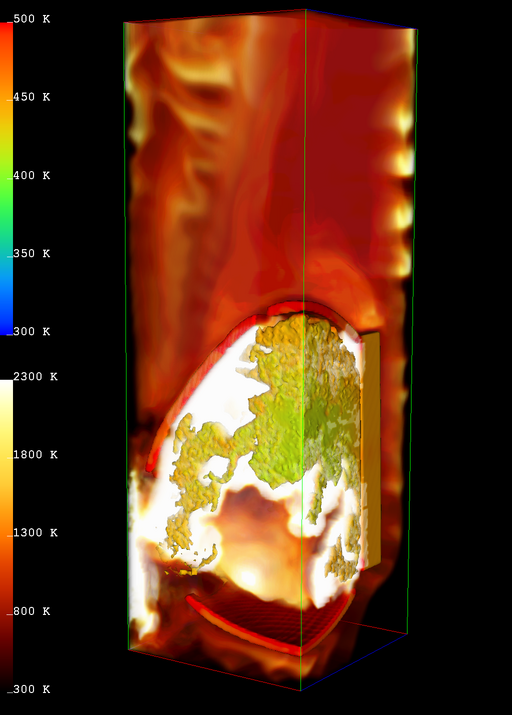
\includegraphics[scale=0.5]{fire-container-explosion-scirun.png}
  \caption{Target Simulation - Fire-Container-Explosion.}
  \label{Fig:fire-container-explosion}
\end{wrapfigure}
%\end{figure}


Complex simulations such as this require both immense computational
power and complex software. Typical simulations include solvers for
structural mechanics, fluids, chemical reactions, and material
models. All of these aspects must be integrated in an efficient manner
to achieve the scalability required to perform these simulations. The
heart of Uintah is a sophisticated computational framework that can
integrate multiple simulation components, analyze the dependencies and
communication patterns between them, and efficiently execute the
resulting multi-physics simulation.  Uintah also provides mechanisms
for automating load-balancing, checkpoint/restart, and parallel
I/O. The Uintah core was designed to be general, and is appropriate
for use in a wide range of PDE algorithms based on structured
(adaptive) grids and particle-in-cell algorithms.


\section{Uintah Software}

The Uintah Computational Framework (also referred to as Uintah or the UCF)
consists of a set of software components and libraries that facilitate
the solution of Partial Differential Equations (PDEs) on Structured
AMR (SAMR) grids using up to hundreds to thousands of processors.

One of the challenges in designing a parallel, component-based and
multi-physics application is determining how to efficiently decompose
the problem domain. Components, by definition, make local
decisions. Yet parallel efficiency is only obtained through a globally
optimal domain decomposition and scheduling of computational
tasks. Typical techniques include allocating disjoint sets of
processing resources to each component, or defining a single domain
decomposition that is a compromise between the ideal load balance of
multiple components. However, neither of these techniques will achieve
maximum efficiency for complex multi-physics problems.

Uintah uses a non-traditional approach to achieving parallelism by
employing an abstract task graph representation to describe
computation and communication. The task graph is an explicit
representation of the computation and communication that occur in the
coarse of a single iteration of the simulation (typically a timestep
or nonlinear solver iteration). Uintah components delegate decisions
about parallelism to a scheduler component by using variable
dependencies to describe communication patterns and characterizing
computational workloads to facilitate a global resource
optimization. The task graph representation has a number of
advantages, including efficient fine-grained coupling of multi-physics
components, flexible load balancing mechanisms and a separation of
application concerns from parallelism concerns. However, it creates a
challenge for scalability which we overcome by creating an implicit
definition of this graph and representing it in a distributed fashion.

%\begin{figure}
%  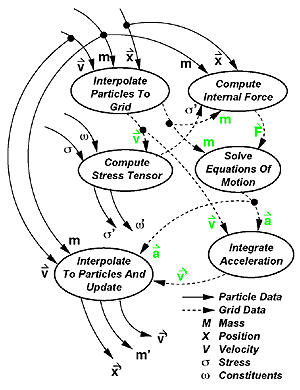
\includegraphics[scale=1]{Taskgraph-diagram.png}
%  \caption{Example Task Graph}
%  \label{fig:TaskGraph}
%\end{figure}

The primary advantage of a component-based approach is that it
facilitates the separate development of simulation algorithms, models,
and infrastructure. Components of the simulation can evolve
independently. The component-based architecture allows pieces of the
system to be implemented in a rudimentary form at first and then
evolve as the technologies mature. Most importantly, Uintah allows the
aspects of parallelism (schedulers, load-balancers, parallel
input/output, and so forth) to evolve independently of the simulation
components. Furthermore, components enable replacement of computation
pieces without complex decision logic in the code itself.

Please see the Developers Guide
(\url{http://www.uintah.utah.edu/trac/chrome/site/UintahAPI.pdf}) for more
information about the internal architecture of Uintah.

\subsection{Software Ports}

Uintah has been ported and runs well on a number of operating
systems.  These include Linux, Mac OSX, Windows, AIX, and HPuX. Simulating
small problems is perfectly feasible on 2-4 processor desktops, while
larger problems will need 100s to 1000s of processors on large
computer clusters. 

\subsection{Uintah Software History}

The UCF was orginally built on top of the SCIRun Problem Solving
Environment.  SCIRun provided a core set of software building blocks,
as well as a powerful visualization package.  While Uintah continues
to use the SCIRun core libraries, Uintah's use of the SCIRun PSE has
been retired in favor of using the VisIt visualization package from
LLNL.


\chapter{Using Uintah} \label{Chapter:UCF}

Several executable programs have been developed using the Uintah
Computational Framework (UCF).  The primary code that drives the
components implemented in Uintah is called \tt sus, \normalfont which
stands for Standalone Uintah Simulation.  The existing components were
originally developed to solve a complex fluid structure problem
involving a container filled with an explosive enveloped in a fire.

The code models the fire and the subsequent heat transfer to the
container followed by the resultant container deformation and ultimate
rupture due to the ignition and burning of the explosive material all
running on thousands of processors requiring thousands of hours of
computer time and hundreds of gigabytes of data storage.  Although
Uintah was developed originally to solve this complicated
multi-physics problem, the general nature of the algorithms and the
framework have allowed researchers to use the code to investigate a
wide range of problems.  The framework is general purpose enough to
allow for the implementation of a variety of implicit and explicit
algorithms on structured grids.  In addition, particle based
algorithms can be implemented using the native particle support found
in the framework.

This code leverages the task based parallelism inherent in the UCF to
implement several time stepping algorithms for structural mechanics,
fluid dynamics, and fluid structure interactions.  What follows is a
description of using \tt sus \normalfont within the realm of
structural mechanics, fluid mechanics, and structure-fluid
interactions.

\section{Installing the Uintah Software}

For information on downloading the Uintah software package (via
tarball or SVN), and how to setup (configure) and build (make) the
system, please refer to the Uintah Installation Guide.

%__________________________________
\section{Mechanics of Running sus}

For single processor simulations, the \tt sus \normalfont executable
(Standalone Uintah Simulation) is run from the command line prompt
like this:
\begin{Verbatim}[fontsize=\footnotesize]
  sus input.ups
\end{Verbatim}
where \tt input.ups \normalfont is an XML formatted input file.  The
Uintah software release contains numerous example input files located
in the \tt src/StandAlone/inputs/UintahRelease \normalfont directory.

For multiprocessor runs, the user generally uses \tt mpirun
\normalfont to launch the code.  Depending on the environment, batch
scheduler, launch scripts, etc, \tt mpirun \normalfont may or may not
be used.  However, in general, something like the following is used:
\begin{Verbatim}[fontsize=\footnotesize]
  mpirun -np num_processors sus -mpi input.ups
\end{Verbatim}

\tt num\_processors \normalfont is the number of processors that will
be used.  The input file must contain a patch layout that has at least
the same number (or greater) of patches as processors specified by a
number following the -np option shown above.

In addition, the \tt -mpi \normalfont is optional but often times
necessary if the mpi environment is not automatically detected from
within the sus executable.

Uintah provides for restarting from checkpoint as well.  For information on
this, see Section~\ref{Sec:DataArchiver}, which describes how to create
checkpoint data, and how to restart from it.

\section{Uintah Problem Specification (UPS)} \label{Sec:UPS}

The Uintah framework uses XML like input files to specify the various
parameters required by simulation components.  These Uintah Problem
Specification (.ups) files are validated based on the specification
found in \tt src/StandAlone/inputs/UPS\_SPEC/ups\_spec.xml \normalfont
(and its sibling files).

The application developer is free to use any of the specified tags to
specify the data needed by the simulation.  The essential tags that
are required by Uintah include the following:

\begin{Verbatim}[fontsize=\footnotesize]
  <Uintah_specification>

  <SimulationComponent>

  <Time>

  <DataArchiver>

  <Grid>
\end{Verbatim}


Individual components have additional tags that specify properties,
algorithms, materials, etc. that are unique to that individual
components.  Within the individual sections on MPM, ICE, MPMICE,
Arches, and MPMArches, the individual tags will be explained more
fully.

The sus executable verifies that the input file adheres to a consistent
specification and that all necessary tags are specified.  However, it
is up to the individual creating or modifying the input file to put in
physically reasonable set of consistent parameters.


\section{Simulation Components} \label{Sec:SimulationComponent}

The input file tag for SimulationComponent has the \tt type \normalfont
attribute that must be specified with either \tt mpm, mpmice, ice, arches,
\normalfont or \tt mpmarches, \normalfont as in:

\begin{Verbatim}[fontsize=\footnotesize]
<SimulationComponent type = "mpm" />
\end{Verbatim}



%__________________________________
\section{Time Related Variables} \label{Sec:TimeRelatedVariables}
Uintah components are time dependent codes.  As such, one of the first
entries in each input file describes the time-stepping parameters.  An
input file segment is given below that encompasses all of the possible
parameters.  The function of each of these parameters is described below.

\begin{Verbatim}[fontsize=\footnotesize]
<Time>
    <maxTime>            1.0         </maxTime>
    <initTime>           0.0         </initTime>
    <delt\_min>           0.0         </delt\_min>
    <delt\_max>           1.0         </delt\_max>
    <delt\_init>          1.0e-9      </delt\_init>
    <max\_delt\_increase>  2.0         </max\_delt\_increase>
    <timestep\_multiplier>1.0         </timestep\_multiplier>
    <max\_Timestep>       100         </max\_Timestep>
    <end\_on\_max\_time\_exactly>true    </end\_on\_max\_time\_exactly>
</Time>
\end{Verbatim}

The following fields are required:

\begin{itemize}
\item maxTime - how long in physical time to run the simulation for
\item initTime - what time to begin the simulation at
\item delt\_min - the smallest timestep the simulation will take
\item delt\_max - the largest timestep the simulation will take
\item timestep\_multiplier - multiplies the timestep by this number (before adjusting to min or max timestep)
\end{itemize}

The following fields are optional:

\begin{itemize}
\item delt\_init - The timestep to take initially (assuming it's less than the one computed by the simulation)
\item initial\_delt\_range - The period of time to use the delt\_init (default = 0)
\item max\_delt\_increase - Maximum amount to multiply the previous delt by (if the newly computed delt is greater than the previous one)
\item max\_iterations - The number of timesteps to run the simulation for (even on a restart)
\item max\_Timesteps - The timestep number to end the simulation on (not usually used with max\_iterations)
\item override\_restart\_delt - On a restart, use this delt instead of the most-recently-used delt.
\item clamp\_timesteps\_to\_output - Sync the delt with the DataArchiver - when an output timestep occurs, reduce the delt to have the time land on the timestep interval (default = false)
\item end\_on\_max\_time\_exactly - clamp the delt such that the last timesteps end on what was specified in maxTime (default = false)
\end{itemize}

A word about timesteps: In general, the timestep (delt) is computed at various stages within a timestep, and the smallest one is used, unless it needs to raise the delt to the delt\_min.




%
%__________________________________
\section{Data Archiver} \label{Sec:DataArchiver}

The Data Archiver section specifies the directory name where data will
be stored and what variables will be saved and how often data is saved
and how frequently the simulation is checkpointed.

The \tt <filebase> \normalfont tag is used to specify the directory
name and by convention, the \tt .uda \normalfont suffix is attached denoting the
``Uintah Data Archive".

Data can be saved based on a frequency setting that is either based on time
intervals;\\
\tt <outputTimestepInterval> integer\_number\_of\_steps </outputTimestepInterval> \normalfont\\
or timestep intervals; \\
\tt <outputInterval> floating\_point\_time\_increment </outputInterval> \normalfont\\

Each simulation component specifies variables with label names that
can be specified for data output.  By convention, particle data are
denoted by \tt p. \normalfont followed by a particular variable name
such as mass, velocity, stress, etc.  Whereas for node based data, the
convention is to use the \tt g. \normalfont followed by the variable
name, such as mass, stress, velocity, etc.  Similarly, cell-centered
and face-centered data typically end with the a trailing \tt CC \normalfont
or \tt FC, \normalfont  respectively.  Within the DataArchiver
section, variables are specified with the following format:

\begin{Verbatim}[fontsize=\footnotesize]
   <save label = "p.mass" />
   <save label = "g.mass" />
\end{Verbatim}

To see a list of
variables available for saving for a given component, execute the following
command from the \tt StandAlone \normalfont directory:

\begin{Verbatim}[fontsize=\footnotesize]
inputs/labelNames component
\end{Verbatim}
where \TT{component} is, e.g., \TT{mpm}, \TT{ice,} etc.

Check-pointing information can be created that provides a mechanism for
restarting a simulation at a later point in time.  The \TT{<checkpoint>}
tag with the \TT{cycle} and \TT{ interval} attributes describe how many
copies of checkpoint data is stored (cycle) and how often it is generated
(interval).  You may also use the \TT{walltimeStart} and \TT{walltimeInterval}
options for specifying when and how offen a checkpoint will be output based
on wall-clock time.

As an example of checkpoint data that has two timesteps worth of
che dckpoint data that is created every .01 seconds of simulation time
are shown below:

\begin{Verbatim}[fontsize=\footnotesize]
<checkpoint cycle = "2" interval = "0.01"/>
\end{Verbatim}
% d

To restart from a checkpointed archive, simply put ``\tt -restart\normalfont" in the
sus command-line arguments and specify the .uda directory instead of
a ups file (sus reads the copied \tt input.xml \normalfont from the
archive).  One can optionally specify a certain timestep to restart
from with \tt -t timestep \normalfont with multiple checkpoints, but the
last checkpointed timestep is the default.  When restarting, sus
copies all of the appropriate information from the old uda directory to its
new uda directory.
% I'M NOT SURE ABOUT THIS, -nocopy REMOVES THE OLD UDA?  I THOUGHT IT
% JUST LEFT STUFF IN THE OLD UDA, WHERE AS -copy MADE A COPY OF OLD TIMESTEP
% DATA, AND -move MOVED THE OLD TIMESTEP DATA TO THE NEW UDA.
%  If one doesn't want to keep the old uda directory
%around, they can specify \tt -nocopy \normalfont to have it be removed
%(e.g., if you are cramped for disk space).  Either way it creates a new uda
%directory for you as always.

Here are some examples:

\begin{Verbatim}[fontsize=\footnotesize]
./sus -mpm -restart disks.uda.000 -nocopy
./sus -mpm -restart disks.uda.000 -t 29
\end{Verbatim}
%
%__________________________________

\section{Simulation Options} \label{Sec:SimulationOptions}


There are many options available when running MPM simulations.  These
are generally specified in the \tt <MPM> \normalfont section of the input file.
A list of these options taken from
\tt inputs/UPS\_SPEC/mpm\_spec.xml \normalfont  is given in section \ref{Sec:UintahImp}.

\section{Geometry objects} \label{Sec:GeometryObjects}

Within several of the components, the material is described by a
combination of physical parameters and the geometry.  Geometry objects
use the notion of constructive solid geometry operations to compose
the layout of the material from simple shapes such as boxes, spheres,
cylinders and cones, as well as operators which include the union,
intersections, differences of the simple shapes.  In addition to the
simple shapes, triangulated surfaces can be used in conjunction with
the simple shapes and the operations on these shapes.

Each geometry object has the following properties, label (string
name), type (box, cylinder, sphere, etc), resolution (vector
quantity), and any unique geometry parameters such as origin, corners,
triangulated data file, etc.  The operators which include, the union,
the difference, and intersection tags contain either lists of
additional operators or the primitives pieces.

As an example of a non-trivial geometry object is shown below:

\begin{Verbatim}[fontsize=\footnotesize]
<geom_object>
     <intersection>
       <box label = "Domain">
          <min>[0.0,0.0,0.0]</min>
          <max>[0.1,0.1,0.1]</max>
       </box>
       <union>
         <sphere label = "First node">
            <origin>[0.022,0.028,0.1  ]</origin>
            <radius>0.01</radius>
         </sphere>
         <sphere label = "2nd node">
            <origin>[0.030,0.075,0.1  ]</origin>
            <radius>0.01</radius>
         </sphere>
       </union>
     </intersection>
     <res>[2,2,2]</res>
     <velocity>[0.,0.,0.]</velocity>
     <temperature>0 </temperature>
</geom_object>
\end{Verbatim}

The following geometry objects are given with their required tags:

\tt box \normalfont has the following tags: min and max which are
vector quantities specified in the \tt [a, b, c] \normalfont format.

\tt sphere \normalfont has an origin tag specified as a vector and the
radius tag specified as a float.

\tt cone \normalfont has a tag for the top and bottom origins (vector)
as well as tags for the top and bottom radius (float) to create a
right circular cone/frustum.

\tt cylinder \normalfont has a tag for the top and bottom origins
(vector) plus a tag for the radius (float).

\tt smoothcyl \normalfont is a geomtry object designed for use with
the cpdi algorithm, which uses a body fit particle spatial
distribution.  This eliminates ``stair-stepped'' boundaries typical of
the standard, grid-based, discretization scheme.  Thus {\it it is
  important to note that this geometry is only designed to work with
  \tt <interpolator>cpdi</interpolator>\normalfont. \it Other
  algorithms may give erroneous answers.}

This geometry has the following tags:

\begin{Verbatim}[fontsize=\footnotesize]
	   <smoothcyl label = "label name">
	     <discretization_scheme> string </discretization_scheme>
	     <bottom> vector </bottom>
	     <top> vector </top>
	     <outer_radius> float </outer_radius>
	     <inner_radius> float </inner_radius>
	     <num_radial> integer </num_radial>
	     <num_axial> integer </num_axial>
	     <num_angular> integer </num_angular>
	     <arc_start_angle> double (in degrees) </arc_start_angle>
	     <arc_angle> double (in degrees) </arc_angle>
	   </smoothcyl>
\end{Verbatim}

The complete or partial annulus or cylinder specified by inner
(optional, defaulting to zero) and outer radii, cylinder axis bottom
and top (all required) and start and final angle (both optional,
defaulting to 0 and 360) will be discretized using planes of
concentric rings of particles.  Particle density is specified by \tt
num\_axial \normalfont and \tt num\_radial\normalfont, the number of
particles in the axial and radial dimensions, respectively
\normalfont.  Note that these particle density specifications
supercede those specified in the \tt <geom\_object> <res> \normalfont
tag, which is ignored.

The required discretization scheme may be either \tt pie\_slices
\normalfont or \tt constant\_particle\_volumes\normalfont.  For the
\tt pie\_slices \normalfont discretization, \tt num\_angular
\normalfont is required to specify the number of particles between \tt
arc\_start \normalfont and \tt arc\_angle \normalfont.  For the \tt
constant\_particle\_volumes \normalfont discretization, the number of
particles between \tt arc\_start \normalfont and \tt arc\_angle
\normalfont is determined individually for each ring of particles by
attempting to keep particle spacings approximately equal in the radial
and angular directions, and thus particle volumes approximately
constant.

End caps may be added to the smoothcyl using the optional \tt
<endcap\_thickness> \normalfont tag, which specifies the axial
dimension of cylinders which are appended to each end of the specified
\tt smoothcyl\normalfont (the radii are the same as the \tt smoothcyl
\normalfont).  Presently, the end cap body fit discretization uses a
legacy scheme.

Note: At the time of writing, multiple \tt smoothcyl \normalfont
geometries within a \tt <geom\_object> \normalfont tag were not
discretized using a body fit particle distribution as described here
(rather the default discretization scheme is used).  This will be
fixed eventually, at which point it may be possible to create more
general endcaps using unions of \tt smoothcyl \normalfont.

\tt ellipsoid \normalfont has an origin tag specified as a vector.  There are
two ways to assign axis lengths depending on the orientation of the ellipsoid.
If the axes are aligned with the Cartesian grid, they may be specified as
floating point values with tagnames: rx, ry, rz.  For all other orientation,
three vector quantities must be specified in the \tt [a,b,c] \normalfont format.
Vector quantity tag names are: v1, v2, v3.These vectors must be orthogonal
to within 1e-12 after dot product or the simulation will throw an exception.
Note, if both vector quantities and floating point tags are used,
the vector quantity inputs will take precedence.

\tt parallelpiped \normalfont requires that four points be specified as
illustrated by the ASCII art snippet taken from the source code:

\begin{Verbatim}[fontsize=\footnotesize]
//********************************************
//                                          //
//                                          //
//       *------------------*               //
//      / \                / \              //
//    P3...\..............*   \             //
//      \   \             .    \            //
//      (z)  P2-----------------*           //
//        \  /             .   /            //
//         \/               . /             //
//         P1-------(x)-----P4              //
//                                          //
//
//  Returns true if the point is inside (or on) the parallelepiped.

\end{Verbatim}

\tt tri \normalfont is a tag for describing a triangulated surface.
The name tag specifies the file name to use for reading in the
triangulated surface description and the points file.  The
triangulated surface (file\_name.tri) contains a list of integers
describing the connectivity of points specified in file\_name.pts.
Here is an excerpt from a tri file and a points file:

\begin{Verbatim}[fontsize=\footnotesize]
Triangulated file

1 39 41
1 41 38
38 41 42
. . .

Points file

0 0.03863 -0.005
0.35227 0.13023 -0.005
0.00403479 0.0296797 -0.005
. . .
\end{Verbatim}
The Mach 2 Wedge example in Section~\ref{Sec:MPMICE_EXAMPLES} depicts usage of
this option.

The boolean operators on the geometry pieces include \tt difference,
intersection, \normalfont and \tt union.\normalfont

The \tt difference \normalfont takes two geometry pieces and subtracts
the second geometry piece from the first geometry piece.  The \tt
intersection \normalfont operator requires at least two geometry
pieces in forming an intersection geometry piece.  Whereas the \tt
union \normalfont operator aggregates a collection of geometry pieces.
Multiple operators can be used to form very complex geometry pieces.

An additional input in the \tt <geom\_object> \normalfont field is the
\tt <res> \normalfont tag.  In MPM, this simply refers to how many particles
are placed in each cell in each coordinate direction.  For multi-material ICE
simulations, the \tt <res> \normalfont serves a similar purpose in that one
can specify the subgrid resolution of the initial material distribution
of mixed cells at the interface of geometry objects.

In addition to the above, it is also possible in MPM simulations to describe
geometry by providing a file containing a series of particle locations.  These
can be in either ASCII or binary format.  In addition, it is also possible to
provide initial data for certain variables on the particles, including
volume, temperature, external force, fiber direction (used in material models
with transverse isotropy) and velocity.  The following is an example in which
external force and fiber direction are specified:

\begin{Verbatim}[fontsize=\footnotesize]
          <file>
              <name>LVcoarse.pts</name>
              <var>p.externalforce</var>
              <var>p.fiberdir</var>
          </file>
\end{Verbatim}

where the text file LVcoarse.pts looks like:

\begin{Verbatim}[fontsize=\footnotesize]
0.0385 0.0335 0.0015 0 0 0 0.248865 -0.0593421 -0.966718
0.0395 0.0335 0.0015 0 0 0 0.254892 -0.0220365 -0.966718
0.0405 0.0335 0.0015 0 0 0 0.267002 0.0197728 -0.963493
0.0415 0.0335 0.0015 0 0 0 0.261177 0.0588869 -0.963493
	.
	.
	.
\end{Verbatim}
Because these files can be arbitrarily large, an additional preprocessing step
must be taken before issuing the \tt sus \normalfont command.
\tt pfs \normalfont for ``Particle File Splitter" is a utility that splits the
data in the \tt .pts \normalfont file into a series of files
(\tt file.pts.0, file.pts.1, \normalfont, etc), one for each
patch.  By doing this, each processor needs only read in the data for the
patches that it contains, rather than each processor reading in the entire file,
which can be hard on the file system.  Note, that this step is required,
even if only using a single patch, and must be reissued any time the patch
configuration is changed.  Usage of this utility, which is compiled
into the \tt StandAlone/tools/pfs \normalfont directory, is:

\begin{Verbatim}[fontsize=\footnotesize]
   pfs input.ups
\end{Verbatim}

One final option is available for initializing particle positions in MPM
simulations, and that is through the use of three dimensional image data,
such as might be collected via CT scans or confocal microscopy.  The image data are provided as 8-bit raw files, and usage in the input file is given as:

\begin{Verbatim}[fontsize=\footnotesize]
        <image>
          <name>spheres.raw</name>
          <res>[1600, 1600, 1600]</res>
          <threshold>[1, 25]</threshold>
        </image>
        <file>
          <name>spheres.pts</name>
          <format>bin</format>
        </file>
\end{Verbatim}

The \tt <image> \normalfont section gives the name of the file, the resolution, in pixels,
in the various coordinate directions, and threshold range.  Particles will be
generated at voxels within the specified range.  The \tt <file> \normalfont
section is the same as that described above.  A different preprocessing utility
is provided when using image data (for the same reasons described previously).
Usage is as follows:

\begin{Verbatim}[fontsize=\footnotesize]
   pfs2 -b input.ups
\end{Verbatim}

The -b indicates that binary \tt spheres.pts.\# \normalfont files will be created, which
saves considerable disk space when performing large simulations.


%__________________________________
\section{Boundary conditions}\label{sec:ucf_bc}

Boundary conditions are specified within the \tt <Grid> \normalfont
but are described separately for clarity.  The essential idea is that
boundary conditions are specified on the domain of the grid.  Values
can be assigned either on the entire face, or parts of the face.
Combinations of various geometric descriptions are used to aid in the
assignment of values over specific regions of the grid.  Each of the
six faces of the grid is denoted by either the minus or plus side of
the domain.

The XML description of a particular boundary condition includes which
side of the domain, the material id, what type of boundary condition
(Dirichlet or Neumann) and which variable and the value assigned.  The
following is a an MPM specification of a Dirichlet boundary condition
assigned to the velocity component on the x minus face (the entire
side) with a vector value of [0.0,0.0,0.0] applied to all of the materials.

\begin{Verbatim}[fontsize=\footnotesize]

 <Grid>
       <BoundaryConditions>
         <Face side = "x-">
             <BCType id = "all" var = "Dirichlet" label = "Velocity">
                   <value> [0.0,0.0,0.0] </value>
             </BCType>
         </Face>
         <Face side = "x+">
            <BCType id = "all" var = "Dirichlet" label = "Velocity">
                 <value> [0.0,0.0,0.0] </value>
            </BCType>
         </Face>
        . . . .
        <BoundaryCondition>
   . . . .
  <Grid>

\end{Verbatim}

The notation \tt <Face side = "x-"> \normalfont indicates that the
entire x minus face of the boundary will have the boundary condition
applied.  The \tt id = "all" \normalfont means that all the
materials will have this value.  To specify the boundary condition for
a particular material, specify an integer number instead of the
"all".  The \tt var = "Dirichlet" \normalfont is used to specify
whether it is a Dirichlet or Neumann or symmetry boundary conditions.
Different components may use the \tt var \normalfont to include a
variety of different boundary conditions and are explained more fully
in the following component sections.  The \tt label = "Velocity"
\normalfont specifies which variable is being assigned and again is
component dependent.  The \tt <value> [0.0,0.0,0.0] </value>
\normalfont specifies the value.

An example of a more complicated boundary condition demonstrating a
hot jet of fluid issued into the domain is described.  The jet is
described by a circle on one side of the domain with boundary
conditions that are different in the circular jet compared to the rest
of the side.

\begin{Verbatim}[fontsize=\footnotesize]

 <Face circle = "y-" origin = "0.0 0.0 0.0" radius = ".5">
        <BCType id = "0"   label = "Pressure" var = "Neumann">
                              <value> 0.0   </value>
        </BCType>
        <BCType id = "0" label = "Velocity" var = "Dirichlet">
                              <value> [0.,1.,0.] </value>
        </BCType>
        <BCType id = "0" label = "Temperature" var = "Dirichlet">
                              <value> 1000.0  </value>
        </BCType>
        <BCType id = "0" label = "Density" var = "Dirichlet">
                              <value> .35379  </value>
        </BCType>
        <BCType id = "0" label = "SpecificVol"  var = "computeFromDensity">
                              <value> 0.0  </value>
        </BCType>
      </Face>
      <Face side = "y-">
        <BCType id = "0"   label = "Pressure"     var = "Neumann">
                              <value> 0.0   </value>
        </BCType>
        <BCType id = "0" label = "Velocity"     var = "Dirichlet">
                              <value> [0.,0.,0.] </value>
        </BCType>
        <BCType id = "0" label = "Temperature"  var = "Neumann">
                              <value> 0.0  </value>
        </BCType>
        <BCType id = "0" label = "Density"      var = "Neumann">
                              <value> 0.0  </value>
        </BCType>
        <BCType id = "0" label = "SpecificVol"  var = "computeFromDensity">
                              <value> 0.0  </value>
        </BCType>
      </Face>

\end{Verbatim}

The jet is described by the circle on the y minus face with the origin
at 0,0,0 and a radius of .5.  For the region outside of the circle,
the boundary conditions are different.  Each side must have at least
the \tt "side" \normalfont specified, but additional circles and
rectangles can be specified on a given face.

An example of the \tt rectangle \normalfont is specified as with the
lower corner at 0,0.181,0 and upper corner at 0,0.5,0.


\begin{Verbatim}[fontsize=\footnotesize]
 <Face rectangle = "x-" lower = "0.0 0.181 0.0" upper = "0.0 0.5 0.0">
\end{Verbatim}

%
%__________________________________
\section{Grid specification} \label{Sec:Grid}

The \tt <Grid> \normalfont section specifies the domain of the
structured grid and includes tags which indicate the lower and upper
corners, the number of extra cells which can be used by various
components for the application of boundary conditions or interpolation
schemes.

The grid is decomposed into a number of patches.  For single processor
problems, usually one patch is used for the entire domain.  For
multiple processor simulations, there must be at least one patch per
processor.  Patches are specified along the x,y,z directions of the
grid using the \tt <patches> [2,5,3] </patches> \normalfont which
specifies two patches along the x direction, five patches along the y
direction and 3 patches along the z direction.  The maximum number of
processors that \tt sus \normalfont could use is $2*5*3 = 30$.
Attempting to use more processors than patches
will cause a run time error during initialization.

Finally, the grid spacing can specified using either a fixed number of
cells along each x,y,z direction or by the size of the grid cell in
each direction.  To specify a fixed number of grid cells, use the \tt
<resolution> [20,20,3] </resolution> \normalfont.  This specifies 20
grid cells in the x direction, 20 in the y direction and 3 in the z
direction.  To specify the grid cell size use the \tt <spacing>
[0.5,0.5,0.3] </spacing> \normalfont.  This specifies the a grid cell
size of .5 in the x and y directions and .3 in the z direction.  The
\tt <resolution> \normalfont and \tt <spacing> \normalfont cannot be
specified together.  The following two examples would generate
identical grids:

\begin{Verbatim}[fontsize=\footnotesize]
<Level>
    <Box label="1">
       <lower>        [0,0,0]          </lower>
       <upper>        [5,5,5]          </upper>
       <extraCells>   [1,1,1]          </extraCells>
       <patches>      [1,1,1]          </patches>
    </Box>
    <spacing>         [0.5,0.5,0.5]    </spacing>
</Level>
\end{Verbatim}

\begin{Verbatim}[fontsize=\footnotesize]
<Level>
    <Box label="1">
       <lower>        [0,0,0]          </lower>
       <upper>        [5,5,5]          </upper>
       <resolution>   [10,10,10]       </resolution>
       <extraCells>   [1,1,1]          </extraCells>
       <patches>      [1,1,1]          </patches>
    </Box>
</Level>
\end{Verbatim}


The above examples indicate that the grid domain has a lower corner at
0,0,0 and an upper corner at 5,5,5 with one extra cell in each
direction.  The domain is broken down into one patch covering the
entire domain with a grid spacing of .5,.5,.5.  Along each dimension
there are ten cells in the interior of the grid and one layer of
``extraCells" outside of the domain.  extraCells are the Uintah nomenclature
for what are frequently referred to as ``ghost-cells".


\section{Schedulers} \label{Sec:Schedulers}

In Uintah, the task scheduler component is responsible for computing task
dependencies, determining the order of task execution and ensuring that the
correct inter-process communication is performed. The Uintah task scheduler
compiles all of the tasks and variable dependencies into a task-graph.
Dependency edges are added between tasks based on the supplied variable
dependencies. The computed dependency edges can be either internal or
external. Internal dependencies are between patches on the same processor and
external dependencies are between patches on different processors. Thus
internal dependencies imply a \emph{necessary order} where external
dependencies specify \emph{required communication}. The compilation process
also combines external dependencies from the same source or to the same
destination, thus coalescing messages.

\vspace{10pt}
\noindent The following is a brief summary of Uintah's available schedulers,
followed by more in-depth discussion of each, its usage and input (XML)
specification.

\begin{itemize}
  \item \textbf{Single Processor Scheduler:} Static task ordering and
      deterministic execution without MPI. Primarily used for small runs on
      a
      single desktop or laptop.
  \item \textbf{MPI Scheduler:} Static task ordering and deterministic
      execution with MPI. One MPI rank per CPU core.
  \item \textbf{Dynamic MPI Scheduler:} Dynamic scheduling with
      non-deterministic, out-of-order execution of tasks at runtime. One MPI
      rank per CPU core.
  \item \textbf{Threaded MPI Scheduler:} A multi-threaded scheduler that
      uses
      a combination of MPI + Pthreads, with dynamic scheduling with
      non-deterministic, out-of-order execution of tasks at runtime. One MPI
      rank per multi-core node. Pthreads are pinned to individual CPU cores
      where these tasks are executed. Uses a centralized model using 1
      control thread and $n-1$ task execution threads. The control thread
      assigns tasks, processes MPI send and recvs. Shared access to the
      DataWarehouse (requires \textbf{MPI\_THREAD\_MULTIPLE} support).
  \item \textbf{Unified Scheduler:} A more advanced, multi-threaded
      scheduler
      that uses a combination of MPI + Pthreads and offers support for GPU
      tasks. Dynamic scheduling with non-deterministic, out-of-order
      execution of tasks at runtime. One MPI rank per multi-core node.
      Pthreads are pinned to individual CPU cores where these tasks are
      executed. Uses a decentralized model wherein all threads can access
      task queues, processes there own MPI send and recvs, with shared
      access
      to the DataWarehouse. (requires \textbf{MPI\_THREAD\_MULTIPLE}
      support)
\end{itemize}

\noindent A comprehensive example of Scheduler input file options with
explanation.

\begin{Verbatim}[fontsize=\footnotesize]
  <Scheduler type="DynamicMPI">
    <small_messages> true </small_messages>
    <taskReadyQueueAlg> MostMessages </taskReadyQueueAlg>
    <VarTracker>
        <start_time> 0.0 </start_time>
        <end_time> 0.2 </end_time>
        <start_index> [0,0,0] </start_index>
        <end_index> [12,12,12] </end_index>
        <var label="divQ" dw="OldDW"/>
        <locations before_comm="false" before_exec="true" after_exec="true"/>
        <task name="Ray::rayTrace"/>
    </VarTracker>
  </Scheduler>
\end{Verbatim}

\begin{itemize}
  \item \emph{Scheduler} - specifies the specific Uintah task scheduler to
      use.
      Valid options are: \TT{SingleProcessor \; MPI \; DynamicMPI \;
      ThreadedMPI \; Unified}
  \item \emph{small\_messages} - whether or not to turn on MPI message
      combination, e.g. send small, individual messages (takes more work to
      organize) or large, combined messages (more communication time). There
      is no "good" value for it. Sometimes MPI message combination works
      better, sometimes not.
  \item \emph{taskReadyQueueAlg} - (only applicable for Dynamic and Unified
      Schedulers) Priority for sorting of tasks in task queues. Valid
      options are: \TT{MostChildren \; LeastChildren \; MostAllChildren \;
      LeastAllChildren \; MostL2Children \; LeastL2Children \; PatchOrder \;
      PatchOrderRandom \; MostMessages \\* LeastMessages \; Random \; FCFS
      \; Stack}. Evidence suggests using \TT{MostMessages} algorithm works 
      best in general. This means highest execution priority is given to 
      tasks that will generate the most outgoing MPI messages.
  \item \emph{VarTracker} - This allows the user to track values for
      variables throughout a simulation or at specific points/ranges in
      time. The elements below control this.
  \vspace{-5pt}
  \item \emph{start\_time} - Variable tracking start time.
  \vspace{-5pt}
  \item \emph{end\_time} - Variable tracking end time.
  \vspace{-5pt}
  \item \emph{start\_index} - Variable tracking starting cell index.
  \vspace{-5pt}
  \item \emph{end\_index} - Variable tracking starting end index.
  \vspace{-5pt}
  \item \emph{var} - Specify the name of the variable to track and the
      DataWarehouse to track from. Valid DataWarehouse options are:
      \TT{NewDW \; OldDW \; CoarseNewDW \; CoarseOldDW \; ParentOldDW \; 
      ParentNewDW}
  \vspace{-5pt}
  \item \emph{locations} - The points in the simulation at which variable
      information will be reported, e.g. before communication and
      before/after task execution.
  \vspace{-5pt}
  \item \emph{task} - The specific task to track the specified variable.
\end{itemize}

\noindent Using the \TT{<Scheduler>} section above in a particular input file,
the Uintah infrastructure will report something like the following at the
beginning of the simulation:

\begin{Verbatim}[fontsize=\footnotesize]
Parallel: 1 MPI process (using MPI)
Parallel: MPI Level Required: 0, provided: 0
Date: Thu Jan 8 16:05:22 2015
Machine: albion
SVN: Revision: 52944
SVN: Last Changed Date: 2015-01-08 09:41:48 -0700 (Thu, 08 Jan 2015)
Assertion level: 3
CFLAGS: -fPIC -fopenmp -Wall -g -O0 -fno-inline-functions
Implicit Solver:      CGSolver
Simulation Component: 'RMCRT_Test'
Load Balancer:        SimpleLoadBalancer
Scheduler:            DynamicMPI

-----------------------------------------------------------
-- Initializing VarTracker...
-- Running from time 0 to 0.2
-- for indices: [int 0, 0, 0] to [int 12, 12, 12]
-- Printing variable information before task execution.
-- Printing variable information after task execution.
-- Tracking variable 'phi' in DataWarehouse 'OldDW'
-- Tracking variables for specific task: Poisson1::timeAdvance
-----------------------------------------------------------
\end{Verbatim}

Do note that you may use the MPI or ThreadedMPI scheduler without ANY of the 
above input file options. By launching \TT{sus} via \TT{mpirun (mpiexec)} will 
invoke the MPI Scheduler automatically; and by launching \TT{sus} via 
\texttt{mpirun (mpiexec)} with the added "\TT{nthreads <n>}" will invoke the 
ThreadedMPI Scheduler automatically. The input file options simply give 
explicit control over what scheduler is used and also makes the Variable 
Tracking capabilities available to a Uintah simulation.


\subsection{Single Processor Scheduler} \label{Sec:SingleProcessorScheduler}
This is the simplest scheduler available within Uintah, and offers static task
ordering and deterministic execution of ALL tasks, without MPI. With this
scheduler, the MPI runtime is not initialized. It is primarily used for small
runs on a single desktop or laptop. The \TT{SingleProcessorScheduler} is not
the default scheduler in any case, and to invoke you must specify
\TT{SingleProcessor} in the \TT{<Scheduler>} section of your input file.


\subsection{MPI Scheduler} \label{Sec:MPIScheduler}
Uintah's MPI Scheduler, shown in Figure \ref{fig:MPIScheduler} is the basic
task scheduler to be used in a distributed, cluster setting. The MPI scheduler
uses a model of one MPI process per core. Though distributed, the task-graph on
each compute node will be identical and is executed in the same order, that is
static task ordering and deterministic execution of ALL tasks. This normally
works well for most cases under roughly 100K cores and where results need to be
reproduced to machine precision.

It has been shown that there is a substantial increase in MPI communication
time at larger numbers of cores due to dependencies between computing tasks
distributed to different nodes and Uintah's memory use associated with ghost
cells and global meta-data. This increase becomes a barrier to scalability
beyond $\mathcal{O}(100K)$ cores. Beyond these core counts you will have to
employ Uintah's Unified Scheduler, described below in Subsection
\ref{Sec:UnifiedScheduler}, which moves to a shared memory model on-node, and
drastically reduces the memory footprint seen at high core counts with an
MPI-only approach.

For most cases, this is the default scheduler, but you may also specify
\TT{MPI} in the \TT{<Scheduler>} section of your input file. An example
command line to use the MPI Scheduler would look like:

\begin{Verbatim}[fontsize=\footnotesize]
mpirun -np <#procs> sus -mpi input.ups
\end{Verbatim}

\begin{figure}[H]
  \centering
  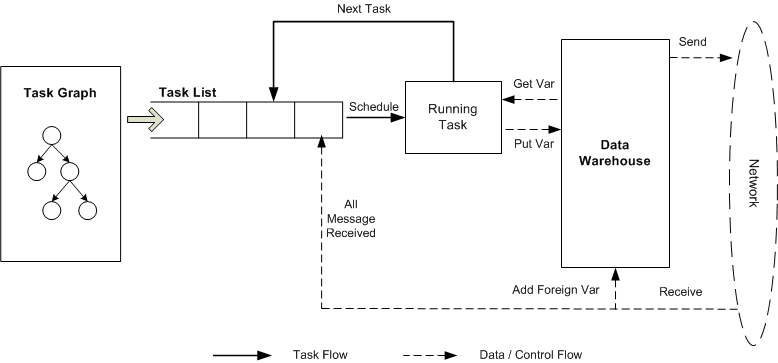
\includegraphics[trim=0cm 0cm 0cm 0cm, clip=true, width=1.0
  \textwidth]{MPIScheduler.png}
  \caption{MPI Scheduler}
  \label{fig:MPIScheduler}
\end{figure}


\subsection{Dynamic MPI Scheduler} \label{Sec:DynamicMPIScheduler} In the MPI
scheduler described above in Subsection \ref{Sec:MPIScheduler}, tasks are
executed in a pre-determined order, which may cause the simulation to sit idle
when a single task is waiting for a message. Measurements have shown that this
type of delay can be nearly 80 percent of the total MPI wait time in Uintah.
The Dynamic MPI scheduler, shown in Figure \ref{fig:DynamicMPIScheduler}
adaptively changes the task order during the execution to overlap communication
and computation. This scheduler achieves a significant performance benefit in
lowering both the MPI wait time and the overall runtime. The dynamic scheduler
utilizes two task queues: an internal ready queue and an external ready queue.
If a task’s internal dependencies are satisfied, then that task will be put in
the internal ready queue where it will wait until all required MPI
communication has finished. A counter of outstanding MPI messages is tracked
for each task. When this counter reaches zero the requisite, external
communication is complete and the task is ready to be executed. At that point
it is placed in the external ready queue (ranked based on the task priority
algorithm used). To invoke the Dynamic MPI Scheduler, you must specify
\TT{DynamicMPI} in the \TT{<Scheduler>} section of your input file. An example
command line to use the Dynamic MPI Scheduler would look like:

\begin{Verbatim}[fontsize=\footnotesize]
mpirun -np <#procs> sus -mpi input.ups
\end{Verbatim}

\begin{figure}[H]
  \centering
  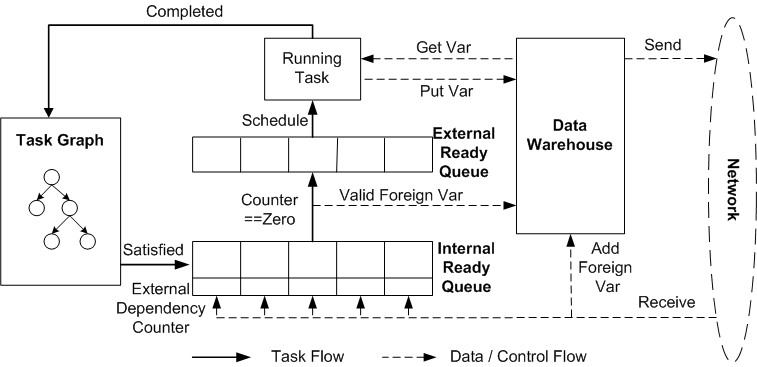
\includegraphics[trim=0cm 0cm 0cm 0cm, clip=true, width=1.0
  \textwidth]{DynamicMPIScheduler.png}
  \caption{Dynamic MPI Scheduler}
  \label{fig:DynamicMPIScheduler}
\end{figure}


\subsection{Threaded MPI Scheduler} \label{Sec:ThreadedMPIScheduler}
At ~100K cores, we have shown that with an MPI-only approach, memory use
associated with ghost cells and global meta-data becomes a barrier to
scalability beyond $\mathcal{O}(100K)$ cores. This limitation has been overcome
within Uintah through the use of hybrid parallelism, significantly reducing the
memory footprint of the code per core by the development of a multi-threaded
task scheduler that takes advantage of current multi-core and emerging
many-core architectures. This hybrid memory approach (a combination of Pthreads
and MPI) has enabled Uintah to demonstrate scalability up to 256K cores on DOE
Titan.

With Uintah's dynamic and static MPI schedulers, based solely on MPI
(Subsections \ref{Sec:MPIScheduler} and \ref{Sec:DynamicMPIScheduler}), data
structures are created on each MPI process. Although most Uintah infrastructure
components are carefully designed to be stored in a distributed manner, it is
necessary for some data to be stored multiple times, e.g. neighboring patch
sets, neighboring tasks and ghost variables. A limitation of pure MPI
scheduling is that tasks which are created and executed on the same node cannot
share data. The multi-threaded Unified scheduler shown in Figure
\ref{fig:UnifiedScheduler} solves this problem by dynamically assigning tasks
to worker threads during execution and share the same infrastructure components
between threads. The architecture of the runtime system has been extended to
support multi-threaded execution (Uintah's answer to \textbf{"MPI + X"}).
Compared to Uintah’s dynamic MPI scheduler, the multi-threaded MPI scheduler
uses a centralized model using 1 control thread and $n-1$ task execution
threads (out of $n$ threads specified). The control thread assigns tasks and
processes MPI recvs (\emph{\textbf{not MPI sends}; worker threads post MPI
sends for the task they execute}). There is shared access to the DataWarehouse.
This scheduler requires \textbf{MPI\_THREAD\_MULTIPLE} support.

\vspace{20pt}
\textbf{NOTE: The ThreadedMPI scheduler is Uintah's default multi-threaded
scheduler.}
\vspace{20pt}

To invoke the ThreadedMPI Scheduler, you must specify \texttt{ThreadedMPI} in
the \TT{<Scheduler>} section of your input file, or simply add the
"\TT{nthreads <n>}" (shown below) to your command to launch the \texttt{sus}
executable.

\begin{Verbatim}[fontsize=\footnotesize]
mpirun -np <#procs> sus -mpi -nthreads 16 input.ups
\end{Verbatim}

Typically the \TT{<n>} will be equal to the number of cores available on a
compute node. The above command line will launch 1 MPI process per node, use 1
control thread and create 15 \TT{(nthreads -1)} additional task execution
threads.

\begin{figure}[H]
  \centering
  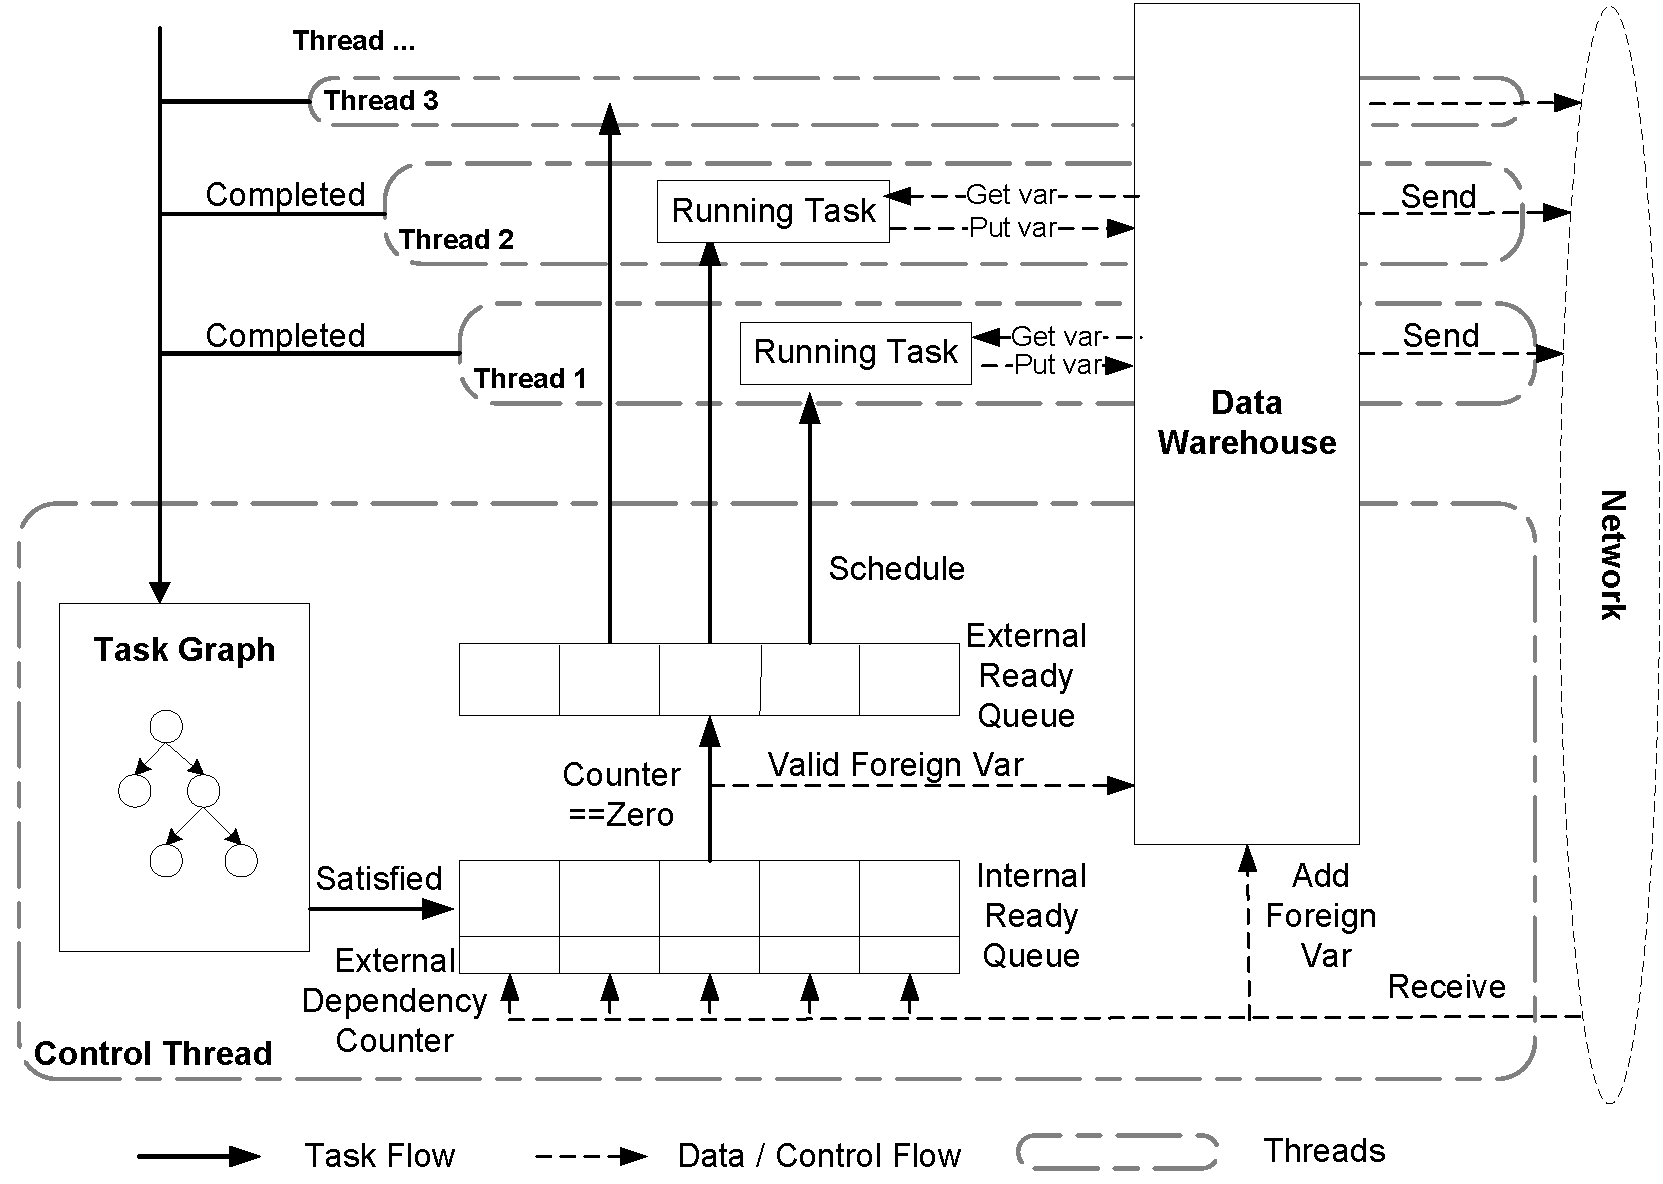
\includegraphics[trim=0cm 0cm 0cm 0cm, clip=true, width=1.0
  \textwidth]{ThreadedMPIScheduler.png}
  \caption{Multi-threaded MPI Scheduler}
  \label{fig:UnifiedScheduler}
\end{figure}


\subsection{Unified Scheduler} \label{Sec:UnifiedScheduler}
Through significant development on the Threaded MPI scheduler (Section
\ref{Sec:ThreadedMPIScheduler} above) Uintah has evolved to demonstrate both
weak and strong scalability up to 768,000 cores on DOE Mira. The hybrid memory
approach used here (a combination of Pthreads and MPI) has enabled Uintah to
demonstrate scalability up to 256K cores on DOE Titan 768k cores on the DOE
Mira system.

The multi-threaded Unified scheduler shown in Figure \ref{fig:UnifiedScheduler}
allows all threads to access task queues (assigning work to themselves) during
execution, process their own MPI sends and recvs, and share the same
infrastructure components between all threads. The architecture of the runtime
system has been extended to support multi-threaded and GPU execution. Compared
to Uintah’s dynamic MPI and Threaded MPI scheduler, the Unified scheduler has
several independent worker threads per MPI process. These all share
infrastructure components such as the regridder, the load balancer, the task
graph and the data warehouse and all have read and write access to them (via
efficient, lock-free data structures). Again, all threads on a node
additionally process their own MPI.

To invoke the Unified Scheduler, you must specify \texttt{Unified} in the
\TT{<Scheduler>} section of your input file, and also add
"\TT{nthreads <n>}" shown below to your command to launch the \texttt{sus}
executable.

\begin{Verbatim}[fontsize=\footnotesize]
mpirun -np <#procs> sus -mpi -nthreads 16 input.ups
\end{Verbatim}

Typically the \TT{<n>} will be equal to the number of cores available on a
compute node. The above command line will launch 1 MPI process per node and
create "\TT{nthreads}" task execution threads.

\vspace{20pt}

\textbf{NOTE: This scheduler is still highly experimental and is under active
development. Documentation on GPU support will be available in a subsequent
Uintah release (1.6.x).}

\begin{figure}[H]
  \centering
  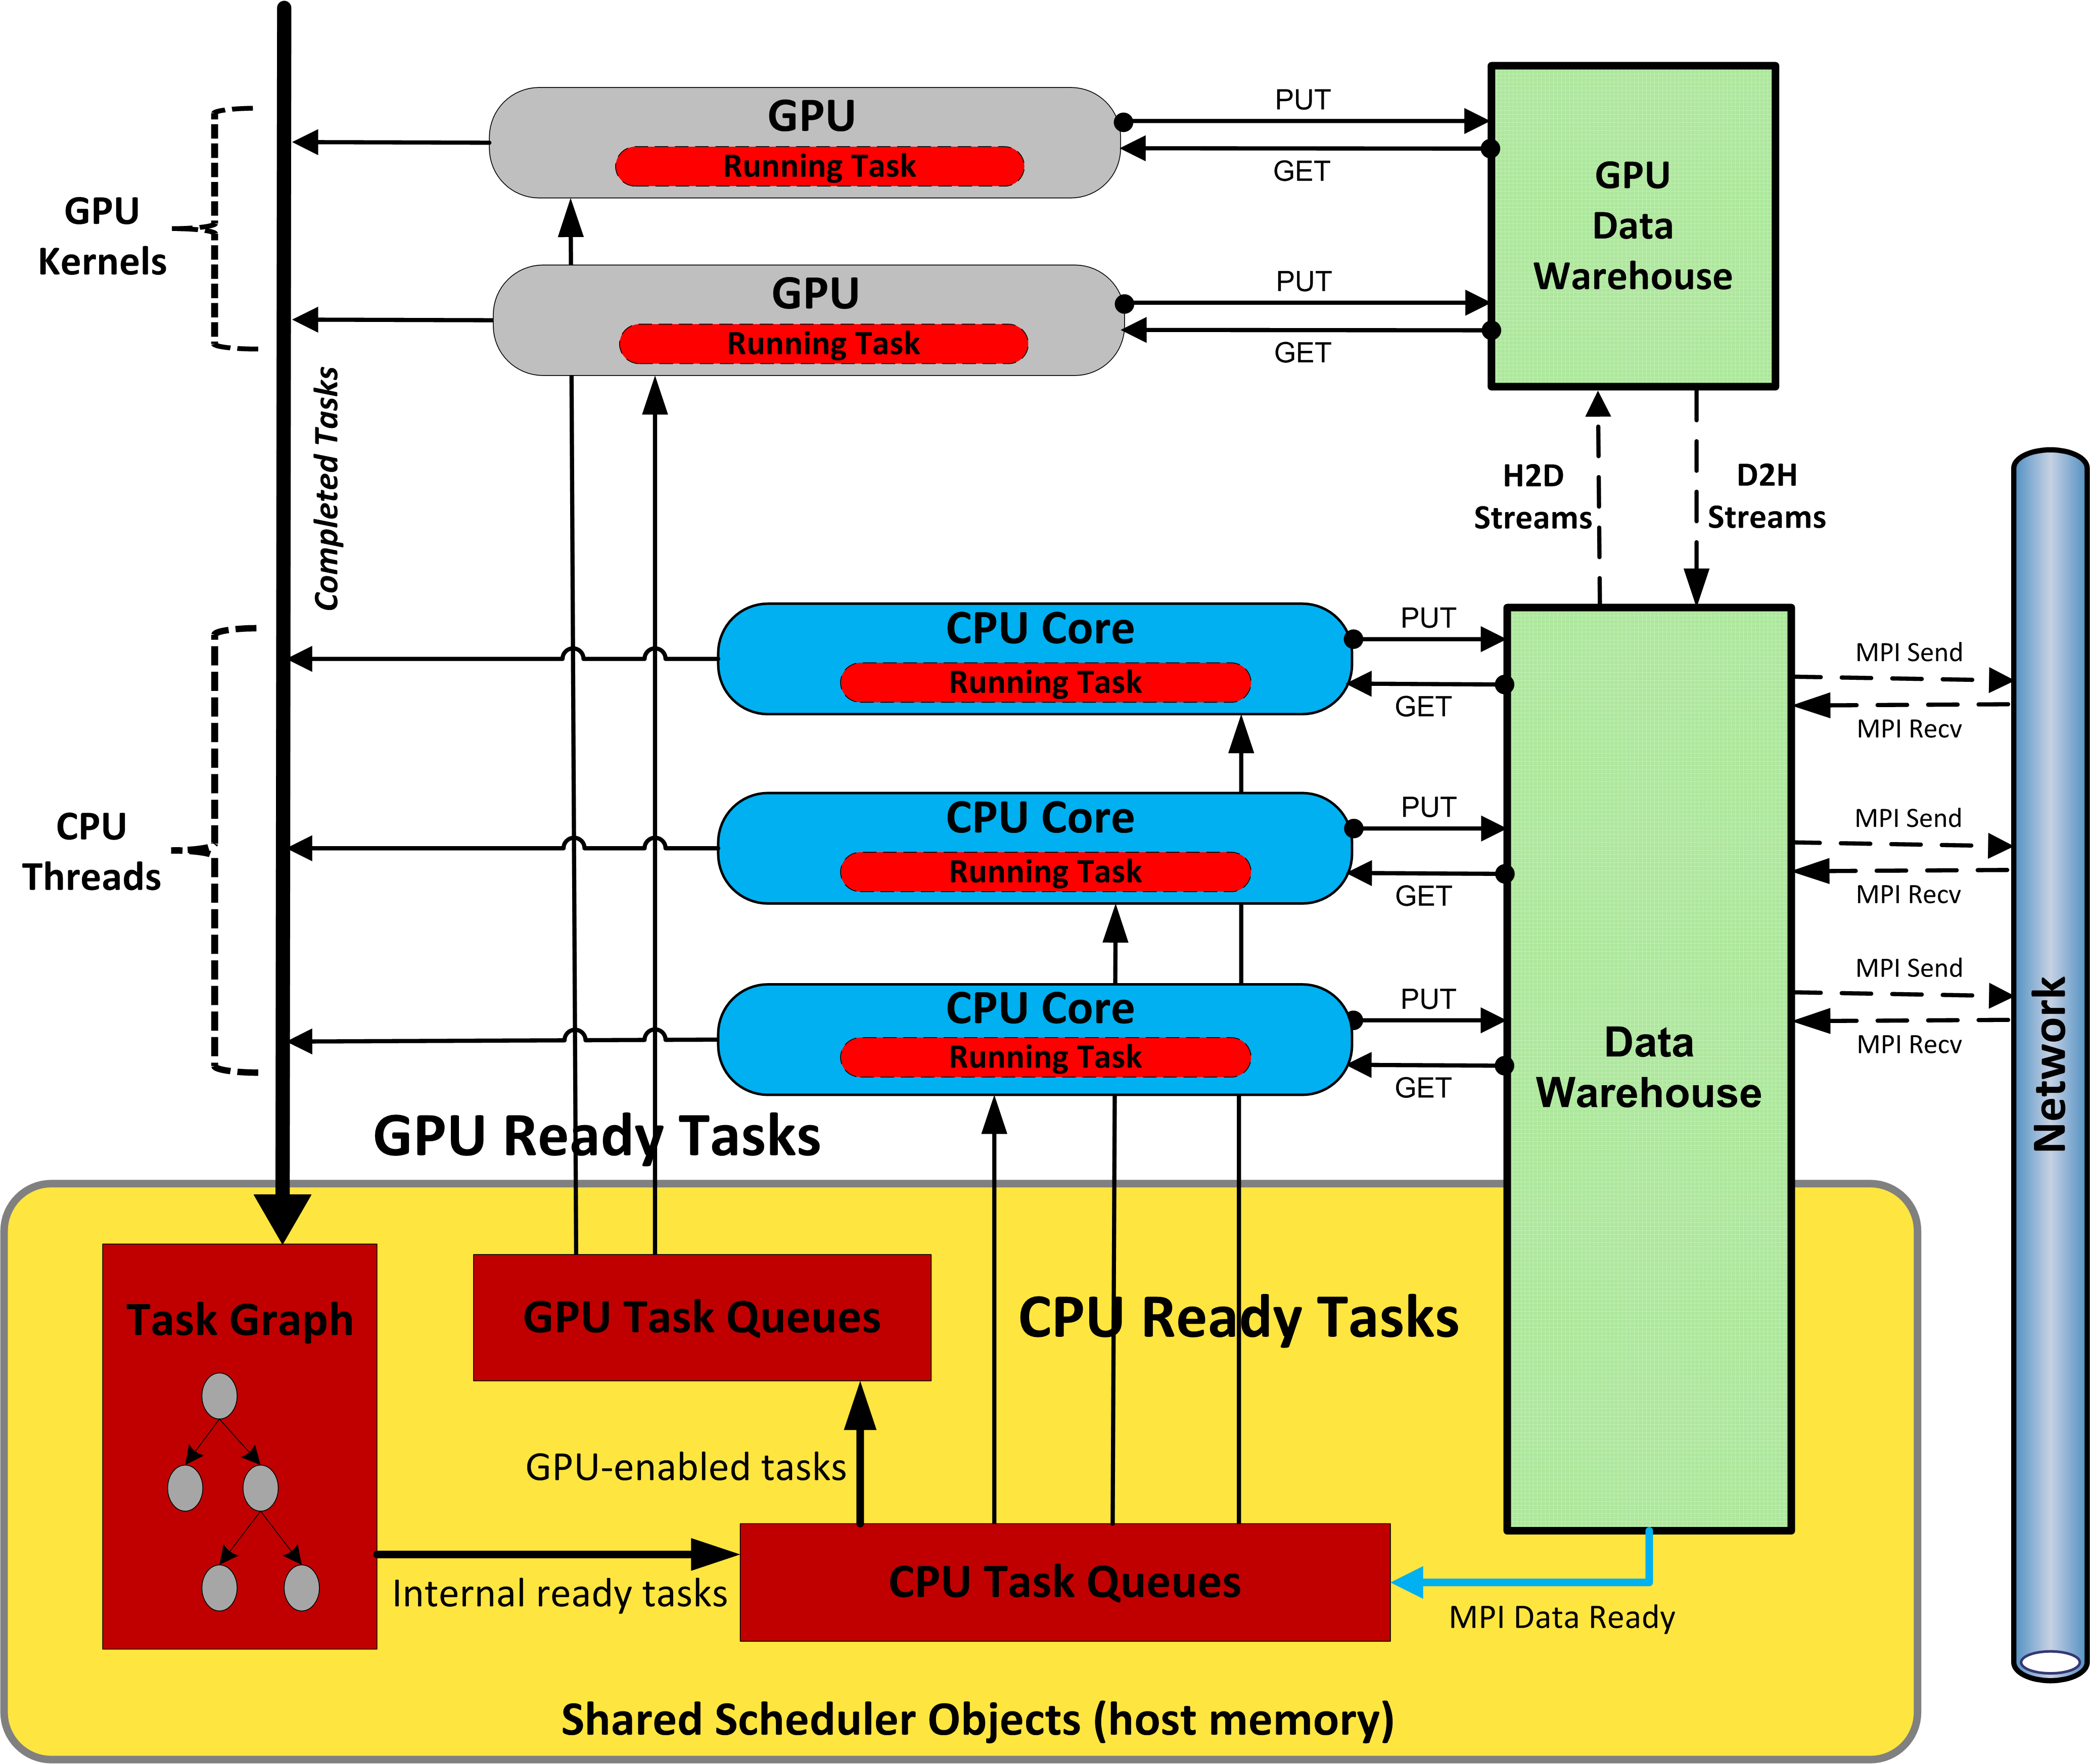
\includegraphics[trim=0cm 0cm 0cm 0cm, clip=true, width=1.0
  \textwidth]{UnifiedScheduler.png}
  \caption{Multi-threaded Unified Scheduler with GPU support}
  \label{fig:UnifiedScheduler}
\end{figure}

%
%__________________________________
%\section{Adaptive Mesh Refinement}
%- Describe refinement flags
%- Describe boundary layers
%- How is a cell flagged as needing to be refined
%
%__________________________________

\section{AMR} \label{Sec:AMR}

In general, the AMR input looks like:

\begin{Verbatim}[fontsize=\footnotesize]
  <AMR>
      <ICE>
        <do_Refluxing>        false    </do_Refluxing>
        <orderOfInterpolation>1         </orderOfInterpolation>
        <Refinement_Criteria_Thresholds>
          <Variable name = "press_CC" value = "1e6" matl = "0" />
        </Refinement_Criteria_Thresholds>
      </ICE>
      <MPM>
        <min_grid_level>-1</min_grid_level>
        <max_grid_level>-1</max_grid_level>
      </MPM>
      <useLockStep>true</useLockStep>    
      <Regridder type="Tiled">
\end{Verbatim}
      %<!--to use hierarchical regridder set the type to "Hierarchical",
       %to use the tiled regridder set the type to "Tiled" -->
       %<type> BNR </type>
\begin{Verbatim}[fontsize=\footnotesize]
        <!--General Regridder Settings-->
        <max_levels>2</max_levels>
        <cell_refinement_ratio>    [[2,2,1]]</cell_refinement_ratio>
        <cell_stability_dilation>   [2,2,1]   </cell_stability_dilation>
        <cell_regrid_dilation>   [1,1,0]   </cell_regrid_dilation>
        <min_boundary_cells>       [1,1,0]   </min_boundary_cells>
\end{Verbatim}     
        %<!--Hierarchical Specific Settings-->
        %<lattice_refinement_ratio> [[4,4,1],[2,2,1]]  </lattice_refinement_ratio>
        
        %<!--Berger Rigoutsos Specific Settings-->
        %<min_patch_size>  [[8,8,1]] </min_patch_size>
        %<patch_ratio_to_target>.2</patch_ratio_to_target>
\begin{Verbatim}[fontsize=\footnotesize]
        <!--Tiled Specific Settings-->
        <min_patch_size>  [[8,8,1]] </min_patch_size>
        <patches_per_level_per_proc>8</patches_per_level_per_proc>         
      </Regridder>
    </AMR>

\end{Verbatim}

When running an ICE simulation, you must specify the following tags in the ICE section of your input deck.

\begin{itemize}
\item do\_refluxing - specifies whether or not to perform refluxing (true or false),
  which equalizes the face values of coarse/fine boundaries between
  levels.
\item orderOfInterpolation - specifies how many coarse cells to use
  when refining the coarse-fine interface (see below).
\item Refinement\_Criteria\_Thresholds section specifies the
  variables whose value will determine where to mark refinement flags,
  see below. Variables need only be specified on adaptive problems.
\item min\_grid\_level (optional) - coarsest level to run ICE on
  (default = 0).
\item max\_grid\_level (optional) - finest level to run ICE on (default
  = max-level -1).

\end{itemize}

If you run an MPM simulation, you must specify the MPM section, and
set min\_grid\_level and max\_grid\_level to the finest level of the
simulation, 0-based (i.e., if there are 2 levels, the level needs to
be set to 1). A shortcut to this is to set min- and max\_grid\_level to
-1.

\begin{itemize}
\item useLockStep - Some simulations require a lock step cycle (mpmice
  and implicit ice), as there has to be inter-level communication in
  the middle of a timestep. See ``W-cycle'' diagram below. Otherwise the
  time refinement ratio will be computed from the cell refinement
  ratio.
\end{itemize}


The presence of the Regridder section specifies you want to run an
adaptive problem.
\begin{itemize}
  \item type (optional) - sets the Regridder type. The options are
   ``Tiled'' (default), ``BNR'' (Berger-Rigoutsos), ``Hierarchical''.
  \red{Only the ``Tiled'' regridder can be used with ICE, AMRICE, MPMAMRICE problems.}
 \item max\_levels - maximum number of levels to create in the grid. 
 \item cell\_refinement\_ratio - How much to refine a cell in each
   dimension. This can be specified in a comma-separated list, with the dimensions in the default order [[x,y,z]].
    \item cell\_stability\_dilation - How much to pad the refinement flags
   in each dimension for stability reasons.  Reset on every timestep. 
 \item cell\_regrid\_dilation - How much to pad the refinement flags in
   each dimension in order to reduce regridding frequency. If the refinement flags are still in the finest level due to large enough padding then regridding will not occur. Reset only when regridding occurs.  
 \item min\_boundary\_cells - The minimum number of cells that needs to
   exist between one level's coarser level and its finer level (i.e.,
   between level 0 and 2).
\end{itemize}

When running a non adaptive problem. Adaptive regridding can be turned off by commenting out the regridding section.
\begin{itemize}
  \item min\_timestep\_interval - The minumum number of timesteps between each regrid. This will not force a regrid but after the set number of timesteps a regrid will be considered. Only used when adaptive regridding is turned off. min\_timestep\_interval $\leq$ cell\_stability\_dilation + 1 
  \item max\_timestep\_interval - The maximum number of timesteps between each regrid.  This will not force a regrid.
 It tells the code it has been a set number of timesteps since the last regrid and it should look at if a regrid is needed. Used primarely when adaptive regridding is turned off.
\end{itemize}

%Hierarchical Specific Settings

%\begin{itemize}
%\item lattice\_refinement\_ratio - Specific to Hierarchical
%  Regridder. Determines how many patches to potentially divide a
 % coarser patch into on the finer level. See Regridding section below.
%\end{itemize}

%Berger-Rigoutsos Specific Settings 

%\begin{itemize}
%\item min\_patch\_size - sets the minimum patch size created by the
%  regridder per level. This size must divide evenly into the
%  resolution and must be divisible by the cell refinement ratio.
%\item patch\_ratio\_to\_target - sets the maximum patch size to the
%  average work load per processor times this value. Theoretical load
%  imbalance should be close to one half of this value. Setting this
%  value too small will create an excess number of patches and cause
%  excessive overhead. .2 seems to be a reasonable value.
%\end{itemize}

Tiled Specific Settings 
\begin{itemize}
\item min\_patch\_size - sets the minimum patch size created by the
  regridder per level. This size must divide evenly into the
  resolution and must be divisible by the cell refinement ratio.
\item patches\_per\_level\_per\_proc - sets the number of patches per
  level per processor that the load balancer attempts to achieve. If
  the number of patches is significantly more than the number
  specified the tiled regridder will increase the tile size by a
  factor of two in order to reduce the number of patches.
\end{itemize}

An example of a simple, 2-dimensional, tiled AMR problem can be found at \tt StandAlone/
inputs/MPMICE/advect\_2L\_MI.ups. \normalfont When the AMR input for this simulation matches the input at the beginning of this section (\ref{Sec:AMR}), we see the following: 

\begin{figure}[H]
  \centering
  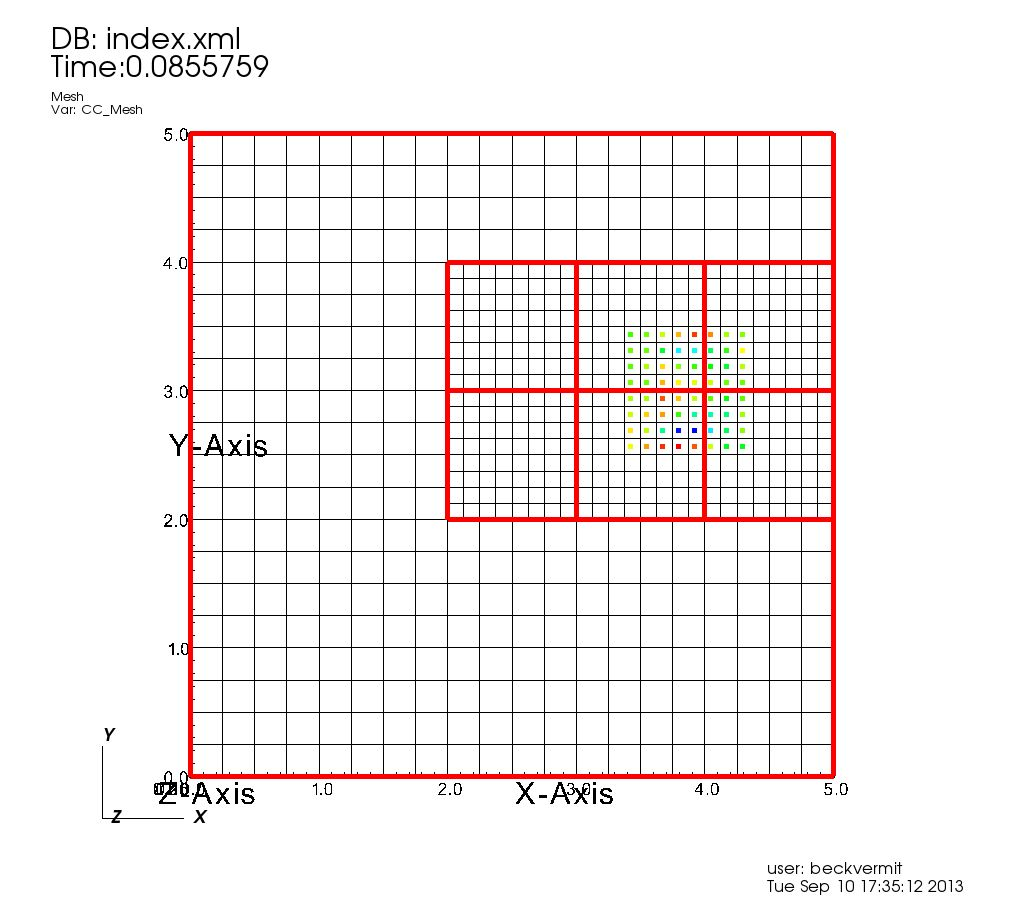
\includegraphics[trim=0cm 3cm 0cm 3cm, clip=true, width=1.\textwidth]{min-patch-size-8-8-1.jpeg}
  \caption{Advect\_2L\_MI with a minimum patch size of [8,8,1]}
  \label{fig:881}
\end{figure}

Here the black lines represent cells and the red lines represent patches with the box of multi-colored points being particles. As can be seen, there are 8 cells per patch in the x and y-direction and only one cell per patch in the z-direction (2D simulation). When we increase the minimum patch size to [20,20,1] we see:

\begin{figure}[H]
  \centering
  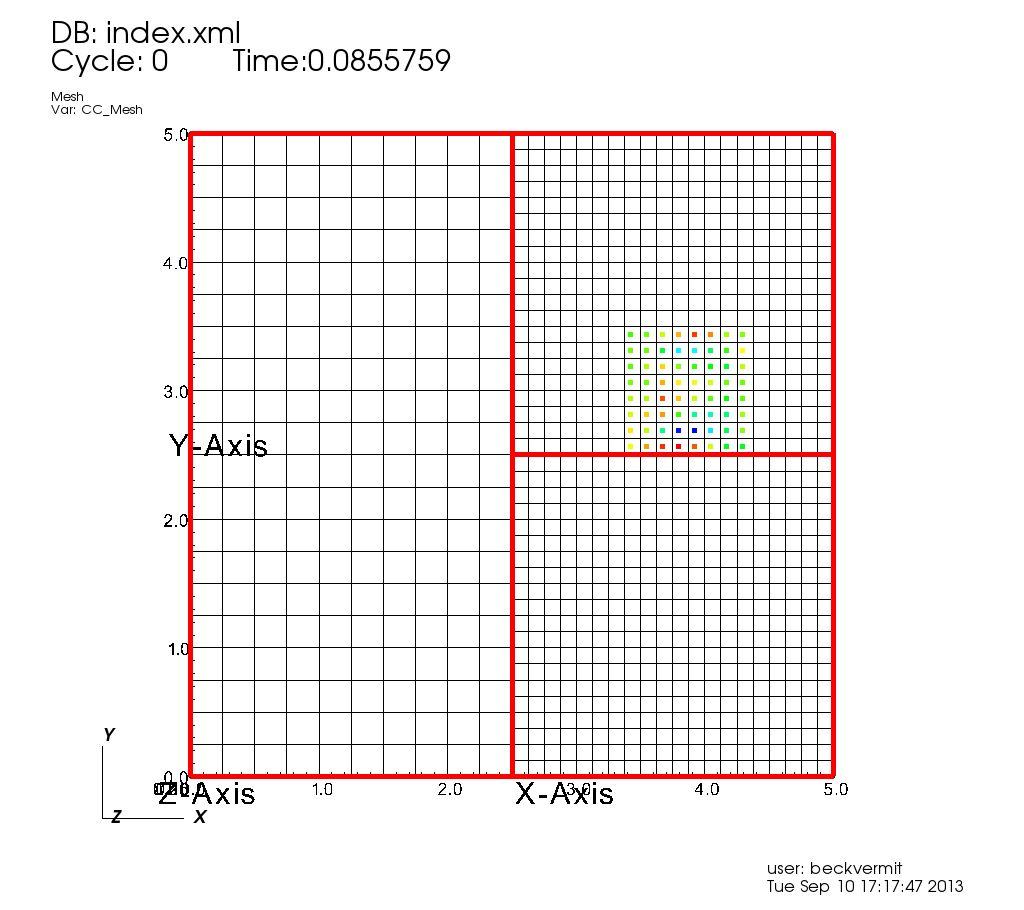
\includegraphics[trim=0cm 3cm 0cm 3cm, clip=true, width=1.\textwidth]{min_patch_size-20-20-1.jpeg}
  \caption{Advect\_2L\_MI with a minimum patch size of [20,20,1]}
  \label{}
\end{figure}

Note that now there are only 2 patches covering our finest level compared to the 6 patches covering our finest levels in figure \ref{fig:881}. This is because there is enough ``padding'' in between our refinement flags and differing levels to avoid setting up whole new patches at the most refined level. This option can be adjusted to increase or decrease the overall amount of regridding necessary with the cell\_regrid\_dilation flag. 

When we decrease our minimum patch size to [4,4,1] we see:
\begin{figure}[H]
  \centering
  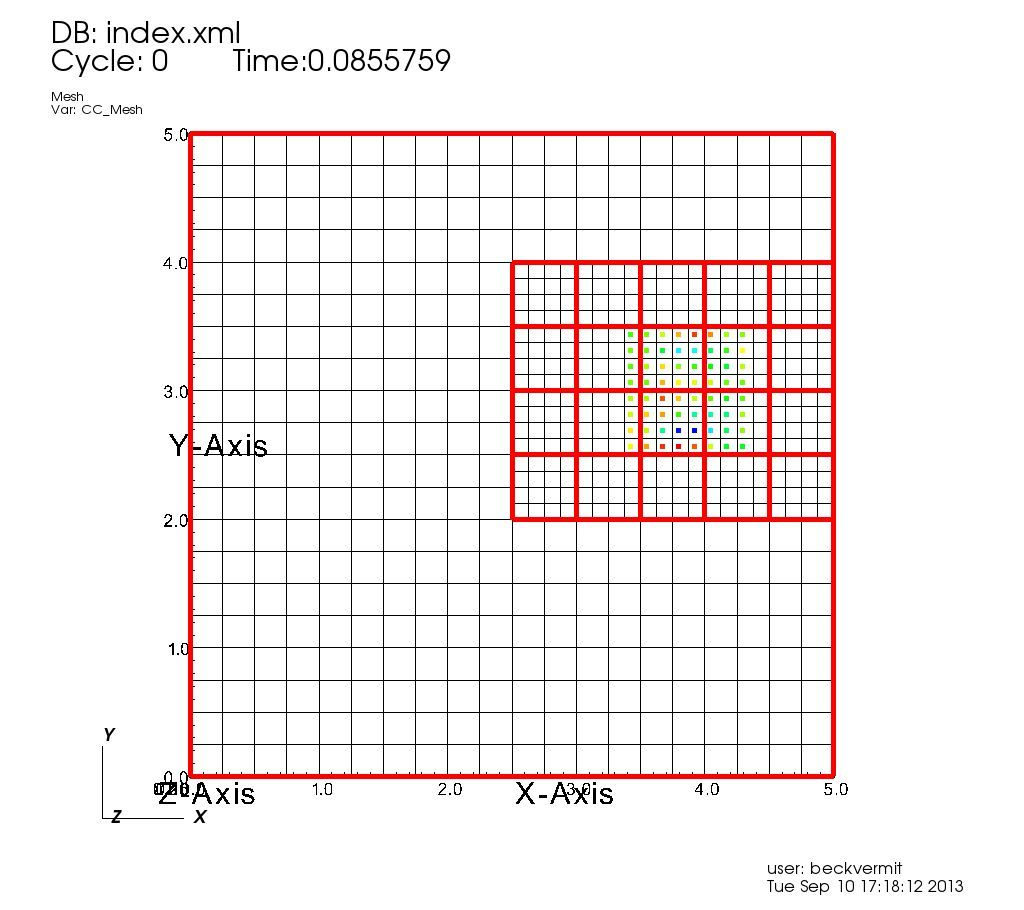
\includegraphics[trim=0cm 3cm 0cm 3cm, clip=true, width=1.\textwidth]{min_patch_size-4-4-1.jpeg}
  \caption{Advect\_2L\_MI with a minimum patch size of [4,4,1]}
  \label{fig:441}
\end{figure}

The best way to increase the ``padding'' of your simulation and therefore decrease the number of regrids required is to increase the cell\_stability\_dilation. Below we see the 2 dimensional example with a minimum patch size of [8,8,1], like figure \ref{fig:881}, but with a cell stability dilation of [10,10,1] rather than [2,2,1].

\begin{figure}[H]
  \centering
  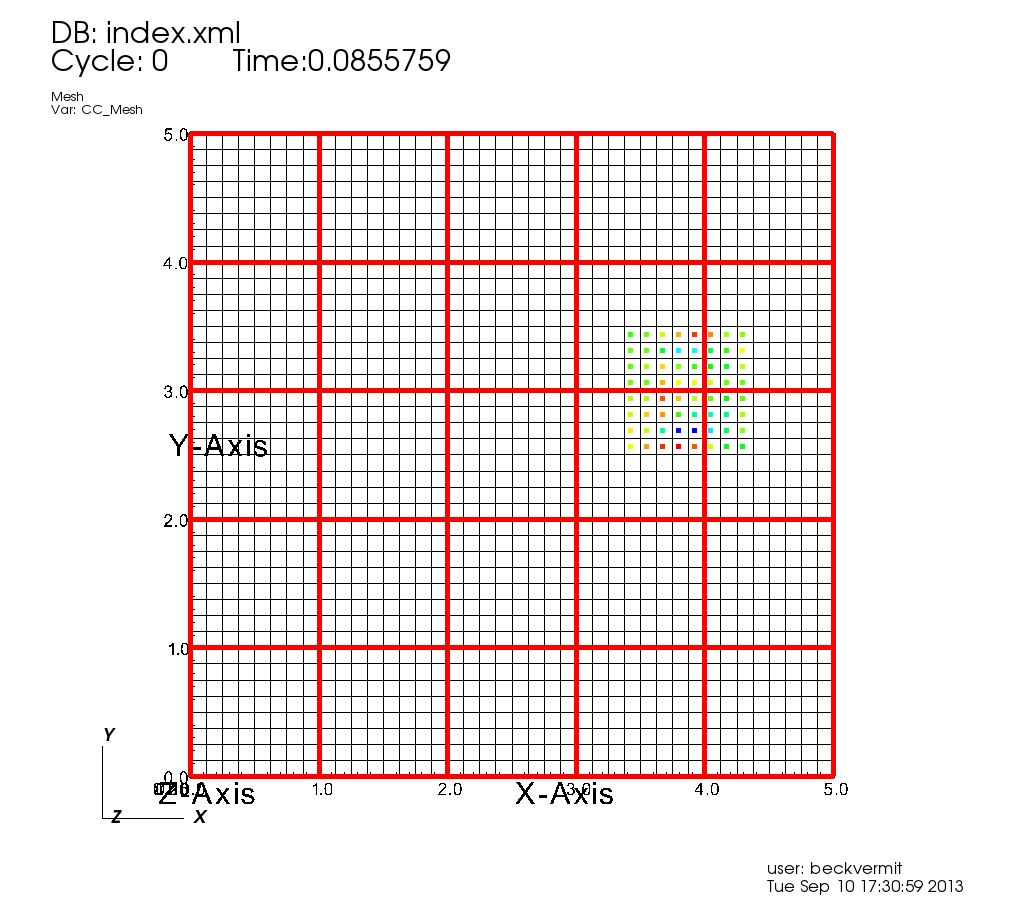
\includegraphics[trim=0cm 3cm 0cm 3cm, clip=true, width=1.\textwidth]{cell_stability_dialation-10-10-1.jpeg}
  \caption{Advect\_2L\_MI with a minimum patch size of [8,8,1] and a cell stability dilation of [10,10,1]}
  \label{fig:10101}
\end{figure}

There is a balance between cell stability dilation and computational time. If your domain is set up like figure \ref{fig:10101}, less computational time will be wasted regridding. However, it could be more economical to utilize some coarser levels in the areas that see little or no particles.
%If you are using the Berger-Rigoutsos regridder you should also
%include a  LoadBalancer, see~\ref{loadbalancer}.


\subsection{AMR Grids}


There are two ways to run with mesh-refinement, either adaptive or
non-adaptive (static). Adaptive grids are created based on the
existence of refinement flags that are created during the
simulation. A regridder will analyze the whole domain, and, wherever there are
refinement flags, construct patches around them on a finer
level. See more on Regridding below.

\subsubsection{Regridding}


For an adaptive problem, specify the Regridder section in the input
file. The Tiled regridder works as follows:
 
%The Hierarchical regridder works as follows: 

%Divide each patch into subpatches according to the
%lattice\_refinement\_ratio. E.g., with a ratio of [2,2,2], it will
%create 8 subpatches. Then, if there are refinement flags within the
%region of that subpatch, then a patch (with resolution increased by
%the cell\_refinement\_ratio) will be added with the subpatch's range on
%the next finer level. This regridder is inefficient and has been
%superseded by the Tiled regridder.

%The Berger-Rigoutsos regridder works as follows: 

%Tiles of the size of the minimum patch size are laid across the next
%finer level. The refinement flags are then used to give each of these
%tiles a single flag indicting if a flag exists within them. The
%Berger-Rigoutsos algorithm is then used to create an initial patch
%set. Next a post processing phase splits patches in order to meet
%alignment constraints. Finally another post process phase splits the
%largest patches further depending on the patch\_ratio\_to\_target input
%file specification. The Berger-Rigoutsos regridder should produce
%patch sets with a much smaller number of patches than the Hierarchical
%Regridder causing less overhead allowing decreasing AMR
%overhead. Unfortunately the cost of the running the BNR algorithm can
%be substantial at large numbers of processors and the patch sets
%produced by this regridder are difficult to load balance. Because of
%this the Tiled regridder should be used.


Tiles sized according to the minimum patch size are laid across domain. Refinement flags are then used to determine which of
those tiles are in the patch set. If the number of tiles is more than
twice the target number of patches then the tile size is doubled in
the shortest dimension. If the number of tiles is less than the target
number of patches then the tile size is halved in the longest
dimension. The tile size will never get smaller than the minimum
specified tile size. This regridder produces regular patch sets that
are easy to load balance. After patches are added, data is stored on them. Then data will be
initialized for those new patches, and in the next timestep, those
patches will be included in the regridding process.

A constraint of the Regridder is that any two patches that share a boundary must be within one level of each other. See (E) and (F) below.

%At initialization time, the regridder can be executed and then the
%problem reinitialized so the problem can be initialized with all
%5max\_levels of refinement.

\begin{figure}[H]
  \centering
  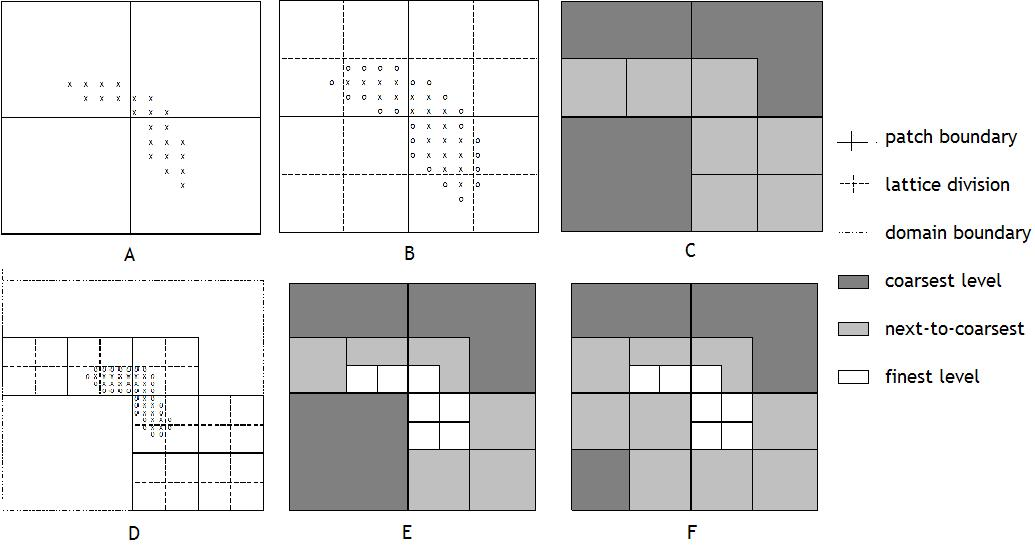
\includegraphics[width=1.\textwidth]{AMR-Regridding.jpg}
  \caption{}
  \label{}
\end{figure}

In the diagram above, image (A) show 4 coarse patches with some marked
error flags. (B) Shows the subpatches for the next level and has the
error flags dilated. (C) Shows the coarse level together with the fine
level you end up with.

(D) During the next regrid, the next level can create error flags as
well. These are some example error flags that are dilated, with the
subpatches for the next level. (E) shows the reulting level with the
other levels. However there are some patch boundaries that span more
than one level. So in (F) we must expand out the middle level to
compensate.

Note that if you you define multiple levels in the input file, all but
the coarsest level will be recycled, and levels will be added where
the Regridder wants to put them.

\subsubsection{Static Grids}

Static grids can be defined by simply not including a Regridder
section in the input file. See the multiple level example in
Grid~\ref{Sec:Grid}.

\subsection{AMR Cycle}

Whether working with an adaptive or a static grid, AMR problems follow
the same cycle. 

In short, there are 3 main AMR operations 
\begin{itemize}

\item Coarsen - This occurs after each execution of a finer level, if
  the time of the finer level lines up with the time of the coarser
  level (see the ``W-cycle'' diagram). Its data are coarsened to the
  coarser level so that the coarse level has a representation of the
  data at the finest resolution. Also as part of this operation is the
  ``reflux'' operations, which to makes the fluxes across the face of
  the coarse-fine boundary consistent across levels.
\item Refine the coarse-fine interface - This occurs after the
  execution of each level and after an associated coarsen (if
  applicable). The cells of the boundary of the finer level are
  interpolated with the nearest cells on the coarser level (so the
  finer level stays in sync with the coarser levels).
\item Refine - This occurs for new patches created by the regrid
  operation. Variables that are necesary will be created on those
  patches by interpolation from the coarser level. 
\end{itemize}

After an entire cycle, then we check to see if we need to regrid. If the flags haven't changed such that patches would form, the grid will remain the same. 

In short, these diagrams may be useful: 

``W-cycle'' (time refinement ratio of 2) 

\begin{figure}[h]
  \centering
  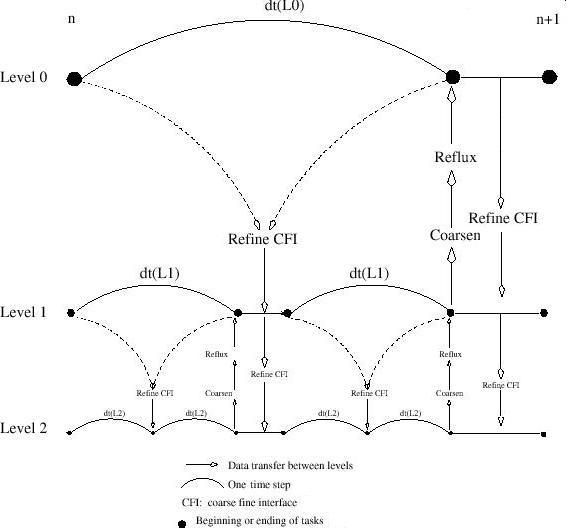
\includegraphics[width=.75\textwidth]{AMR-Cycle-W.jpg}
  \caption{}
  \label{}
\end{figure}

``Lockstep cycle''

\begin{figure}[h]
  \centering
  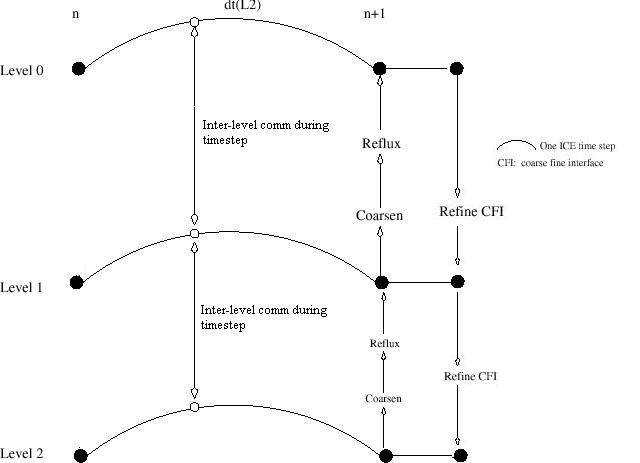
\includegraphics[width=.75\textwidth]{AMR-Cycle-Lock.jpg}
  \caption{}
  \label{}
\end{figure}

\section{Regridder}

The regridder creates a multilevel grid from the refinement flags.
Each level will completely cover the refinement flags from the coarser
level.  The primary regridder used in Uintah is the \TT{Tiled} regridder.
The tiled regridder creates a set of evenly sized tiles across the domain
that will become patches if refinement is required in the tiles region.

The following is an example of this regridder.

\begin{Verbatim}[fontsize=\footnotesize]
<Regridder type="Tiled">
    <max_levels>2</max_levels>
    <cell_refinement_ratio> [[2,2,1]] </cell_refinement_ratio>
    <cell_stability_dilation> [2,2,0] </cell_stability_dilation>
    <min_boundary_cells> [1,1,0] </min_boundary_cells>
    <min_patch_size>  [[8,8,1]] </min_patch_size>
</Regridder>
\end{Verbatim}

The \TT{max\_levels} tag specifies the maximum number of levels
to be created.  The \TT{cell\_refinement\_ratio} tag specifies the
refinement ratio between the levels.  This can be specified on a per
level basis as follows:

\begin{Verbatim}[fontsize=\footnotesize]
    <cell_refinement_ratio> [[2,2,1],[4,4,1]] </cell_refinement_ratio>
\end{Verbatim}

The \TT{cell\_stability\_dilation} tag specifies how many cells around
the refinement flags are also guaranteed to be refined.  The
\TT{min\_boundary\_cells} tag specifies the size of the boundary layers.
The size of the tiles is specified using the \TT{min\_patch\_size} tag
and can also be specified on a per level basis.

%
%__________________________________
\section{Dynamic Load Balancing}

Uintah has a couple of load balancing options which may be useful for increasing performance by decreasing
the load imbalance.  The following describes the loadbalancer section of an input file and what effects
it has on the load balancer.  

If no load balancer is specified then a simple load balancing method which assigns an equal number of patches
to processors. This is not ideal in most cases and should be avoided.

\subsection{Input File Specs}
\begin{Verbatim}[fontsize=\footnotesize]
   <LoadBalancer type="DLB"> 
        <!-- DLB specific flags -->
        <costAlgorithm>ModelLS</costAlgorithm>
        <hasParticles>true</hasParticles>

        <!-- DLB/PLB flags -->
        <timestepInterval>25</timestepInterval>
        <gainThreshold>0.15</gainThreshold>
        <outputNthProc>1</outputNthProc>
        <doSpaceCurve>true</doSpaceCurve>

   </LoadBalancer>
\end{Verbatim}

There are two main load balancers used in Uintah.  The first is the DLB load balancer.
This is a robust load balancer that is good for many problems.  In addition,
this load balancer can utilize profiling in order to tune itself during the runtime
in order to achieve better results.  

To use this load balancer the user must specify the type as "DLB".  It is also suggested
that the user specify a costAlgorithm which can be "Model", "ModelLS", "Memory", or
"Kalman" with the default being "ModelLS".  If "hasParticles" is set to true then
these cost algorithms will take the number of particles into account when determining
the cost.

This algorithm first orders the patches linearly.  If doSpaceCurve is set to true
then this ordering is done according to a Hilbert Space-Filling curve, which will
likely provide better clusterings.  Once the patches are ordered linearly, costs
are assigned to each patch and the patches are distributed onto processors so that
the costs on each processor are even.  

The PLB load balancer is an alterantive to the DLB load balancer which is
likely more efficent for particle based calculations.  This load balancer
divides the patches into two sets (cell dominate and particle domintate), 
which is determined using the particleCost and cellCost parameters.
The particle dominate patches are then assigned to processors while trying
to equalize the number of particles on each processor.  Finally the 
cell dominate patches are assigned to patches in order to equalize the number
of cells while accounting for the number of cells already assigned during 
the particle assignment phase.  This method can also utilize a space-filling
curve.  

The following list describes other flags utilized by these load balancers:
\begin{itemize}
  \item timestepInterval - how many timesteps must pass before reevaluating the load balance.  
  \item gainThreshold - the predicted percent improvement that is required to reload balance.  
  \item outputNthProc - output data on only every Nth processor (experimental). 
\end{itemize}



%__________________________________
\section{UDA}

%\subsection{UDA Directory Structure}

The UDA is a file/directory structure used to save Uintah simulation
data.  For the most part, the user need not concern himself with the
UDA layout, but it is a good idea to have a general feeling for how
the data is stored on disk.

%\subsubsection{UDA Naming}

Every time a simulation (sus) is run, a new UDA is created.  Sus uses
the $<$filebase$>$ tag in the simulation input file to name the UDA
directory (appending a version number).  If an UDA of that name
already exists, the next version number is used.  Additionally, a
symbolic link named ``disks.uda'' (is updated to and) will point to
the newest version of this simulations UDA.  Eg:

\begin{Verbatim}[fontsize=\footnotesize]
disks.uda.000
disks.uda.001
disks.uda.001 <- disks.uda
\end{Verbatim}

%\subsubsection{UDA Files}

Each UDA consists of a number of top level files, a checkpoints
subdirectory, and subdirectories for each saved timestep.  These files
include:

\begin{itemize}

\item \tt.dat \normalfont files contain global information about the
  simulation (each line in the .dat files contains: simulation\_time
  value).
\item \tt checkpoints \normalfont directory contains a limited
  number of time step data subdirectories that contain a complete
  snapshot of the simulation (allowing for the simulation to be
  restarted from that time).
\item \tt input.xml \normalfont contains the original problem
  specification (the .ups file).
\item \tt index.xml \normalfont contains information on the actual
  simulation run.
\item \tt t0000\# \normalfont contains data saved for that specific
  time step.  The data saved is specified in .ups file and may be a
  very limited subset of the full simulation data.

\end{itemize}

The 'validateUda' script (src/Packages/Uintah/scripts/) can be used to
test the integrity of a UDA directory. It does not interogate the data
for 'correctness', but it performs 5 basic tests on each uda:

\begin{Verbatim}
Usage validateUda  <udas>
Test 0:  Does index.xml exist?                                        true or false
Test 1:  Does each timestep in index.xml exist?                       true or false
Test 2:  Do all timesteps.xml files exist?                            true or false
Test 3:  Do all the level directories exist:                          true or false
Test 4:  Do all of the pxxxx.xml files exist and have size >0:        true or false
Test 5:  Do all of the pxxxx.data files exist and have size > 0:      true or false
\end{Verbatim}

If any of the tests fail then the corrupt output timestep should be removed from the index.xml file.


See Section~\ref{Sec:DataArchiver} for a description of how to specify
what data are saved and how frequently.

% The following seems not that useful to me.  JG
%Example UDA file list:

%CenterOfMassPosition.dat
%CenterOfMassVelocity.dat
%KineticEnergy.dat
%StrainEnergy.dat
%TotalMass.dat
%checkpoints
%index.xml
%input.xml
%t00001
%t00057

%\subsection{Known Issues}

%Occasionally, due (most likely) to file system issues on large
%clusters, some of the files in the UDA have been found to be corrupted
%or nonexistent.  (There is error checking in the code to try to
%prevent this.  We believe that either the OS/File system is
%incorreclty returning error codes, or, more likely, that the files are
%corrupted (due to file system issues) after the simulation is done.

%\subsection{Restarting}

%The sus executable provides a mechanism for checkpointing the code and
%then restarting the ongoing simulation from a given checkpoint.



%__________________________________
\chapter{Visualization tools -- VisIt}

Visualization of Uintah data is currently possible using any of two
software packages.  These are SCIRun and VisIt.  Of these, SCIRun is
no longer supported, although legacy versions will continue to work.
The VisIt package from LLNL is general purpose visualization software
that offers all of the usual capabilities for rendering scientific
data.  It is still developed and maintained by LLNL staff, and its
interface to Uintah data is supported by the Uintah team.

%Manta offers volume rendering and particle visualization based on
%parallel (shared memory) ray tracing techniques.  While the
%capabilities of Manta are more limited, it is a fast way to
%interactively interrogate reasonably large datasets, provided the user
%has access to a reasonable shared memory resource, (e.g. an 8 core
%desktop system).


\section{Reading Uintah Data Archives}

\begin{wrapfigure}{r}{.50\textwidth}
  \vspace{-30pt}
  \begin{center}
    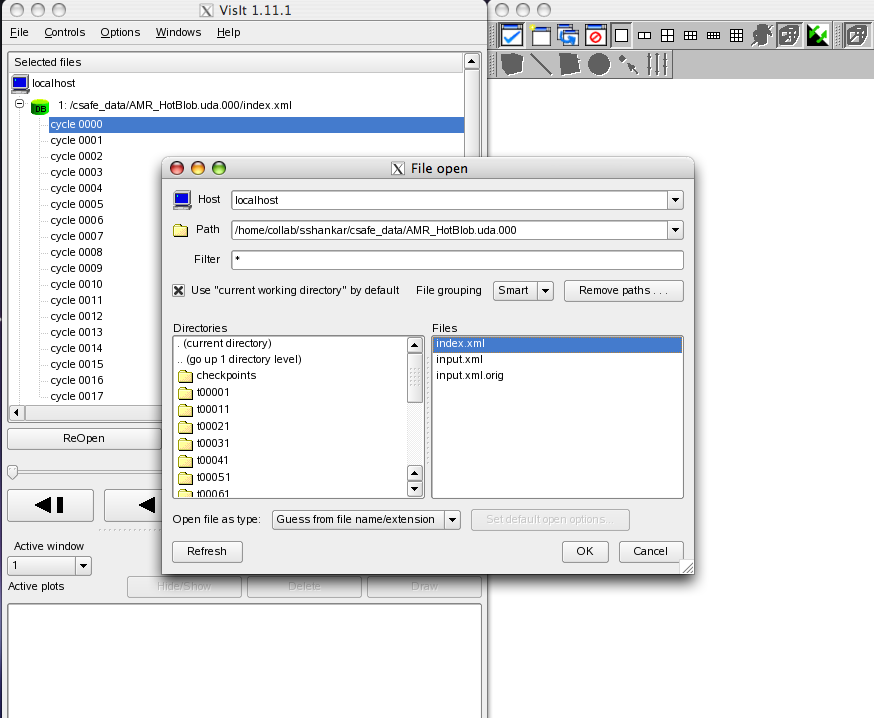
\includegraphics[width=.3\textwidth]{VisItFileOpen.png}
  \end{center}
  \vspace{-20pt}
  \caption{Opening an UDA with VisIt}
  \vspace{-10pt}
  \label{VisItFileOpen}
\end{wrapfigure}


Once you have installed VisIt and the UDA reader plugin, you can
launch VisIt and start visualizing UDA's. To open a UDA, select \tt
Open File \normalfont from the \tt File \normalfont menu. Browse into
the UDA you want to load and select the \tt index.xml \normalfont
file. Then hit on \tt OK \normalfont and a list of timesteps should
now appear on the gui. Figure~\ref{VisItFileOpen} illustrates this
process.


\section{Plots}

\begin{wrapfigure}{r}{.50\textwidth}
  \vspace{-65pt}
  \center
  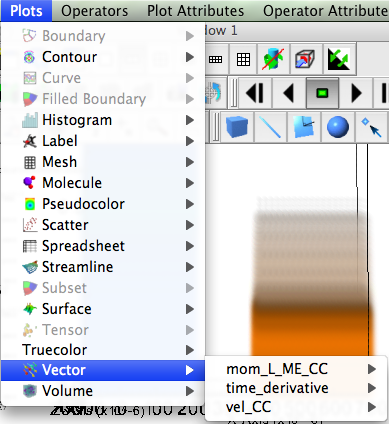
\includegraphics[width=.3\textwidth]{VisItPlots.png}
  \vspace{-10pt}
  \caption{Various plots in VisIt}
  \vspace{-50pt}
  \label{VisItPlots}
\end{wrapfigure}


VisIt displays data as plots. A plot might render a specific variable
or it might render the structure of the mesh. Figure~\ref{VisItPlots}
illustrates this.


Note that VisIt attempts to analyze the variables and associate them
with the appropriate plots. As shown in Figure~\ref{VisItPlots}, only
vector variables are available for the vector plot. The most commonly
used plots for visualizing UDA's are Pseudocolor, Volume and the
Vector plot. The Subset plot can be used to visualize the structure of
patches in an AMR dataset.
%The Mesh plot can be used to display the mesh structure.

\begin{wrapfigure}{r}{.50\textwidth}
  \vspace{-20pt}
  \center
  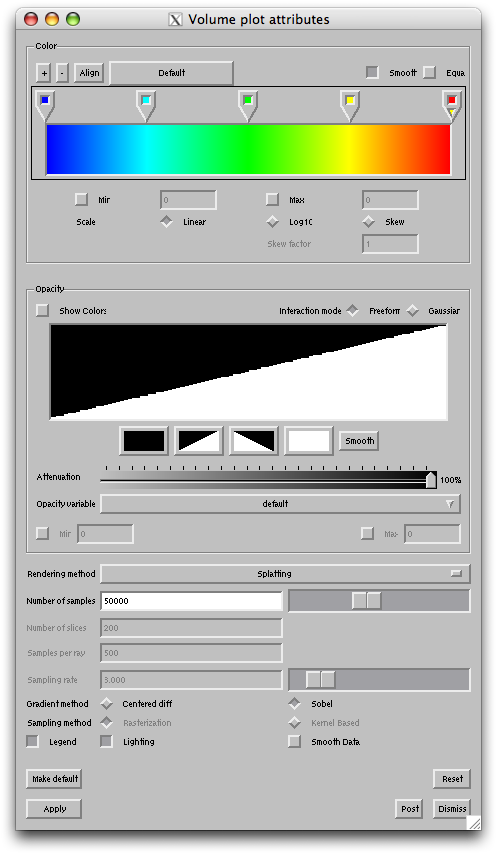
\includegraphics[width=.30\textwidth]{VisItVolumeAtts.png}
  \vspace{-10pt}
  \caption{Volume plot attributes in VisIt}
  \vspace{-40pt}
  \label{VisItVolumeAtts}
\end{wrapfigure}


Once you have a plot, you change plot attributes by clicking on the
PlotAtts menu and selecting the plot of you choice. Alternatively, you
may double click on the plot itself in Active plots window. For
example, if you have a Volume plot and you want to change its
attributes, the window shown in Figure~\ref{VisItVolumeAtts} pops up.



As seen in Figure~\ref{VisItVolumeAtts}, you can change the color map,
opacity curve, rendering method, no. of samples, lighting options,
etc. in this window.



\section{Operators}

\begin{wrapfigure}{r}{.50\textwidth}
  \vspace{-20pt}
  \center
  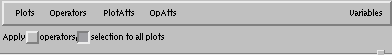
\includegraphics[width=.3\textwidth]{VisItApplyOperators.png}
  \vspace{-10pt}
  \caption{Unchecking "selection to all plots"}
  \vspace{-10pt}
  \label{VisItApplyOperators}
\end{wrapfigure}


A wide variety of operators can be applied to the plots, as mentioned
earlier. These modify the incoming datasets in some way (eg., a slice
formats a 3D dataset into a 2D slice), which can then be
plotted. However, you will first need to select a plot and then only
you can apply an operator to it (though the order of operation is
opposite). An important thing to keep in mind is that when you select
an operator, by default it gets applied to all the plots in the Active
plots window. You will need to uncheck the Apply operators checkbox,
in case you just want to apply the operator to a single plot as shown
in Figure~\ref{VisItApplyOperators}.


The entire list of operators that VisIt supports can be seen by
clicking on the Operators menu. Also, once you have applied an
operator, you can change its attributes by clicking on the OpAtts menu
and then clicking on the desired operator.
Figures~\ref{VisItSelectPlot} and~\ref{VisItSelectOperator} illustrate
how you can apply a Slice operator to a Pseudocolor plot and then
change the operator attributes.  First, apply the Pseudocolor plot to
a desired variable, and then select the Slice operator from the
Operators menu.

% \begin{wrapfigure}{r}{.50\textwidth}
%   \vspace{-10pt}
%   \center
%   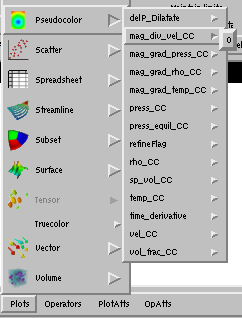
\includegraphics[width=.3\textwidth]{VisItSelectPlot.png}
%   \caption{Applying the Pseudocolor plot to a variable}
%   \vspace{10pt}
%   \label{VisItSelectPlot}
% \end{wrapfigure}


% \begin{wrapfigure}{r}{.50\textwidth}
%   \center
%   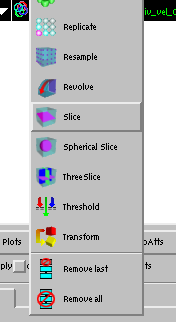
\includegraphics[width=.3\textwidth]{VisItSelectOperator.png}
%   \caption{Applying an operator to a plot}
%   \label{VisItSelectOperator}
% \end{wrapfigure}


\begin{figure}
  \vspace{-100pt}
  \centering
  \subfloat[Applying the Pseudocolor plot to a variable]{\label{VisItSelectPlot}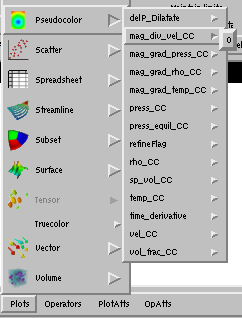
\includegraphics[width=0.3\textwidth]{VisItSelectPlot.png}}
  \hspace{50pts}
  \subfloat[Applying an operator to a plot]{\label{VisItSelectOperator}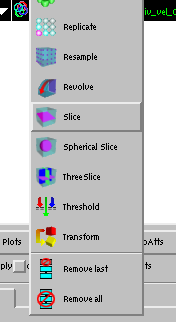
\includegraphics[width=0.3\textwidth]{VisItSelectOperator.png}}
  \caption{}
  \label{}
\end{figure}


\begin{figure}
  \centering
  \vspace{-20pt}
  \subfloat[Ordering of an operator and a plot]{\label{VisItOrderOperator}
  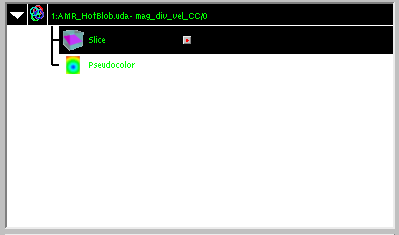
\includegraphics[width=.3\textwidth]{VisItOrderOperator.png}}
  \hspace{50pt}
  \subfloat[Slice plot attributes in VisIt]{\label{VisItSliceAtts}
  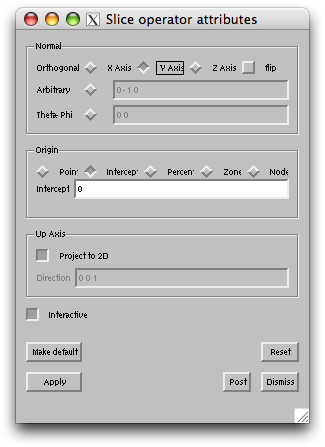
\includegraphics[width=.3\textwidth]{VisItSliceAtts.png}}
  \caption{}
  \label{}
\end{figure}

% \begin{wrapfigure}{R}{.50\textwidth}
%   \center
%   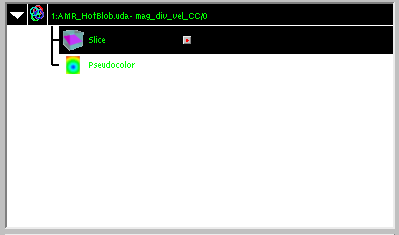
\includegraphics[width=.3\textwidth]{VisItOrderOperator.png}
%   \caption{Ordering of an operator and a plot}
%   \label{VisItSliceAtts}
% \end{wrapfigure}

At this point in time, you should have an ordering similar to that in
Figure~\ref{VisItOrderOperator}.  Once you have this order, select
Slice from the OpAtts menu. This will pop up the Slice operator
attributes window, as shown in Figure~\ref{VisItSliceAtts}.

% \begin{wrapfigure}{r}{.50\textwidth}
%   \center
%   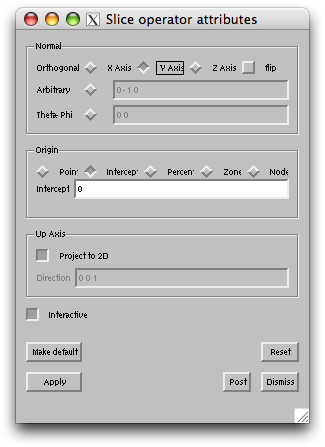
\includegraphics[width=.4\textwidth]{VisItSliceAtts.png}
%   \caption{Slice plot attributes in VisIt}
%   \label{VisItSliceAtts}
% \end{wrapfigure}

You can now play up with the various attributes (eg., selecting normal
plane) to obtain the desired visualization. The checkbox "Project to
2D" should be unchecked is you want to have the slice in 3D space.

\section{Vectors}

\begin{wrapfigure}{r}{.50\textwidth}
  \center
  \vspace{-40pts}
  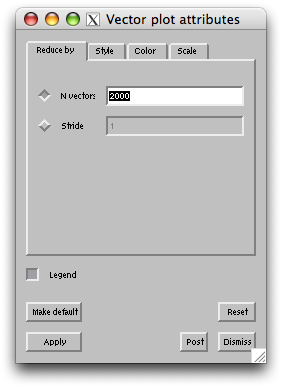
\includegraphics[width=.48\linewidth]{VisItVectorNumber.png}
  \caption{Increasing the number of Vectors}
  \vspace{-20pts}
  \label{VisItVectorNumber}
\end{wrapfigure}


By default, VisIt reduces the number of vectors plotted (to 400) and
this needs to be manually changed to the original number or something
greater, only if required.  This can be accomplished by changing the
attributes of the Vector plot. In Figure~\ref{VisItVectorNumber}, the
number of vectors has been increased to 2000.


\begin{wrapfigure}{r}{.50\textwidth}
  \center
  \vspace{-50pts}
  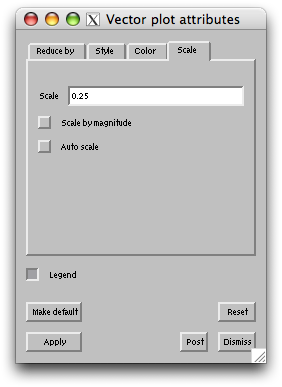
\includegraphics[width=.3\textwidth]{VisItVectorScale.png}
  \caption{Increasing the scale of Vectors}
  \vspace{-30pts}
  \label{VisItVectorScale}
\end{wrapfigure}


Also if you would like all the vectors to be visible, you would need
to switch off both the options, \tt Scale by magnitude \normalfont and
\tt Auto scale \normalfont under the Scale tab in the same window as
shown in figure~\ref{VisItVectorScale} describes this.


\section{AMR datasets}



AMR datasets are read the same way as single level datasets. Once you
have it read, you can apply an plot/ operator on it. Since the dataset
is organized as levels and patches, you now have the flexibility of
visualizing each of them independently or as in a group. To achieve
this (assuming that you have already selected a plot), click on the
Subset button either on the Active Plots window in the gui or on the
same option in the Controls menu. This is illustrated in
Figures~\ref{VisItSubsetIcon} and ~\ref{VisItSubsetWin}.

% \begin{wrapfigure}{r}{100mm}
%   \center
%   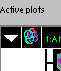
\includegraphics[width=.5\linewidth]{VisItSubsetIcon.png}
%   \caption{Clicking on this icon pops up the Subset window}
%   \label{VisItSubsetIcon}
% \end{wrapfigure}

% \begin{wrapfigure}{r}{100mm}
%   \center
%   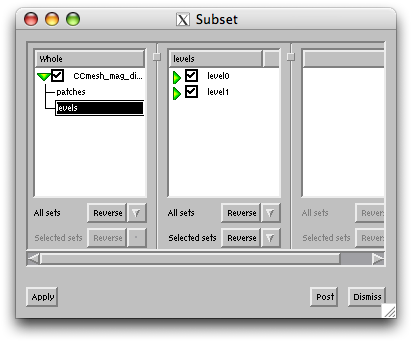
\includegraphics[width=.5\linewidth]{VisItSubsetWin.png}
%   \caption{The Subset window in VisIt}
%   \label{VisItSubsetWin}
% \end{wrapfigure}

\begin{figure}
  \centering
  \vspace{-80pt}
  \subfloat[Clicking on this icon pops up the Subset window]{\label{VisItSubsetIcon}
  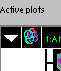
\includegraphics[width=.3\linewidth]{VisItSubsetIcon.png}}
  \hspace{50pt}
  \subfloat[The Subset window in VisIt]{\label{VisItSubsetWin}
  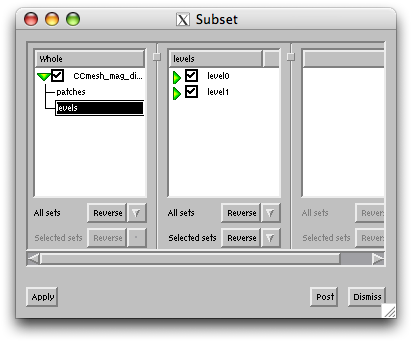
\includegraphics[width=.3\linewidth]{VisItSubsetWin.png}}
  \caption{}
  \vspace{-10pt}
  \label{}
\end{figure}


\section{Examples}

\subsection{Volume visualization}

\begin{enumerate}

\item Read in the uda by selecting the index.xml file. A list of
  timesteps should now appear on the gui.

% \begin{wrapfigure}{r}{.50\textwidth}
%   \center
%   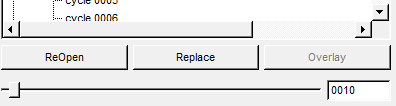
\includegraphics[width=.3\textwidth]{VisItTimestepBox.png}
%   \caption{The window on the gui lists all the timesteps}
%   \label{VisItTimestepBox}
% \end{wrapfigure}


\item The first timestep (cycle 0000) should be preselected. In case you
are interested in plotting a different timestep, just double click on
it. Alternatively you can type it in the small rectangular box
(Figure~\ref{VisItTimestepBox}), just below the list of
timesteps. This can also be done at a later period in time, when you
are done plotting the variable associated with a specific timestep and
want to traverse through the others.


\item Next we select a variable to plotted. We click on the Plots
  menu, select the Volume plot and then select the variable tempIN as
  shown in the Figure~\ref{VisItVolumeTempINATK08}. The number '1'
  refers to the material associated with the variable.

% \begin{wrapfigure}{r}{.50\textwidth}
%   \center
%   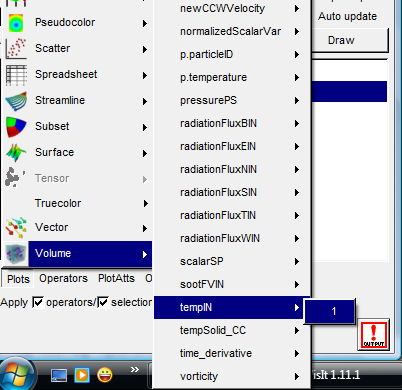
\includegraphics[width=.3\textwidth]{VisItVolumeTempINATK08.png}
%   \caption{Selecting a volume plot and an associated variable/ material}
%   \label{VisItVolumeTempINATK08}
% \end{wrapfigure}

\item The variable tempIN/1 now appears on the Active plots window
  (Figure~\ref{VisItDrawTempINATK08}). Select the variable and click
  Draw.

\begin{figure}[h]
  \centering
  \vspace{-10pt}
  \subfloat[The window on the gui lists all the timesteps]{\label{VisItTimestepBox}
  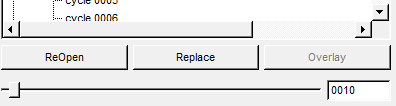
\includegraphics[width=.3\textwidth]{VisItTimestepBox.png}}
  \hspace{10pt}
  \subfloat[Selecting a volume plot and an associated variable/ material]{\label{VisItVolumeTempINATK08}
  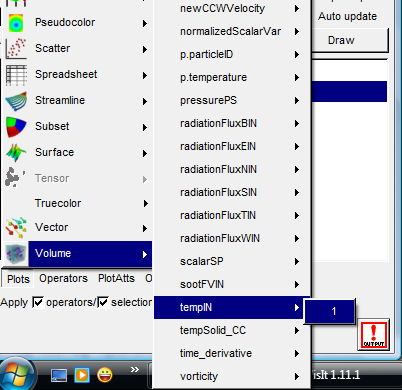
\includegraphics[width=.3\textwidth]{VisItVolumeTempINATK08.png}}
  \hspace{10pt}
  \subfloat[The list of plots in the Active plots window]{\label{VisItDrawTempINATK08}
  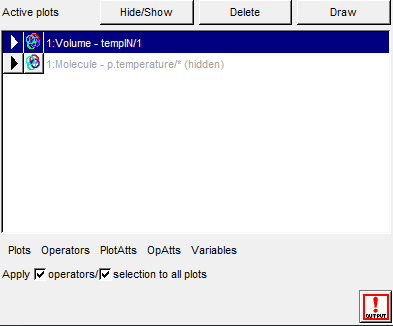
\includegraphics[width=.3\textwidth]{VisItDrawTempINATK08.png}}
  \caption{}
  \vspace{-10pt}
  \label{}
\end{figure}




% \begin{wrapfigure}{r}{.50\textwidth}
%   \center
%   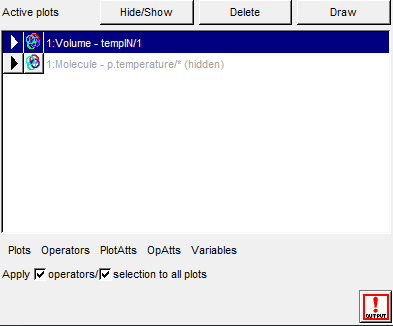
\includegraphics[width=.4\textwidth]{VisItDrawTempINATK08.png}
%   \caption{The list of plots in the Active plots window}
%   \label{VisItDrawTempINATK08}
% \end{wrapfigure}

\item A visualization now appears on the Viewer window, as shown in
  Figure~\ref{VisItVolumeTempINATK08Viewer}. You can interact with the
  visualization in terms of rotating it (holding the left mouse button
  and dragging it), zooming in/ out (scrolling the roller on the mouse
  and/ or selecting the magnifier at the top of the Viewer window)
  etc.



% \begin{wrapfigure}{r}{.50\textwidth}
%   \center
%   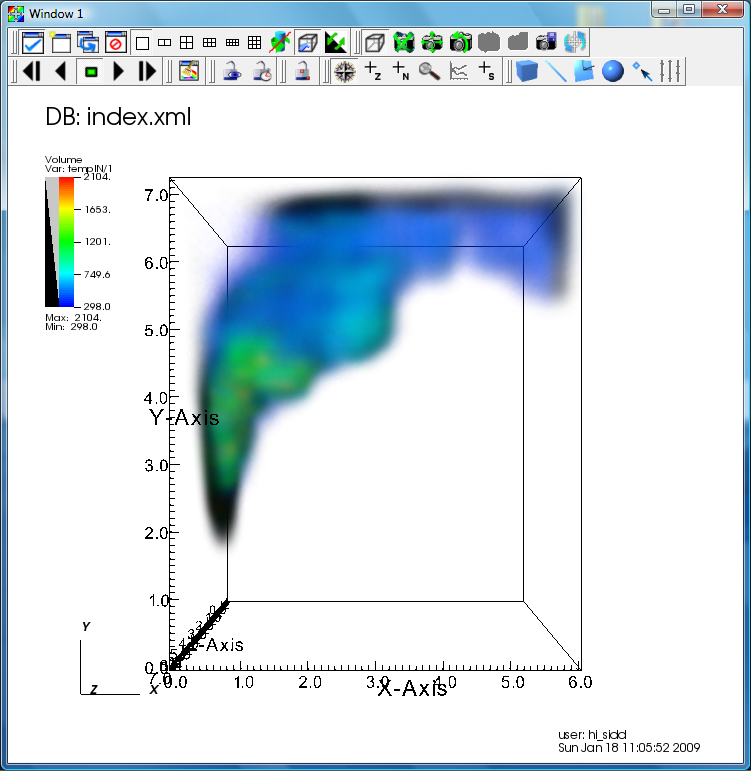
\includegraphics[width=.4\textwidth]{VisItVolumeTempINATK08Viewer.png}
%   \caption{Visualization of a volume on the viewer window}
%   \label{VisItVolumeTempINATK08Viewer}
% \end{wrapfigure}

\item Once you have this basic volume visualization, you can change
  its attributes by double clicking on the Volume - tempIN/1 plot in
  the Active plots window. This pops up the Volume plot attributes
  window (Figure~\ref{VisItVolumeAttributes1} and
  figure~\ref{VisItVolumeAttributes2}).

% \begin{wrapfigure}{r}{.50\textwidth}
%   \center
%   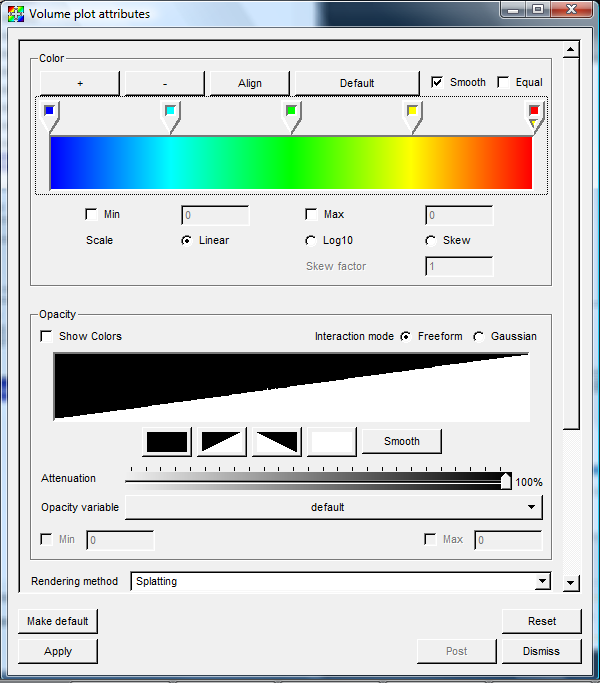
\includegraphics[width=.4\textwidth]{VisItVolumeAttributes1.png}
%   \caption{Volume visualization attributes window}
%   \label{VisItVolumeAttributes1}
% \end{wrapfigure}

% \begin{wrapfigure}{r}{.50\textwidth}
%   \center
%   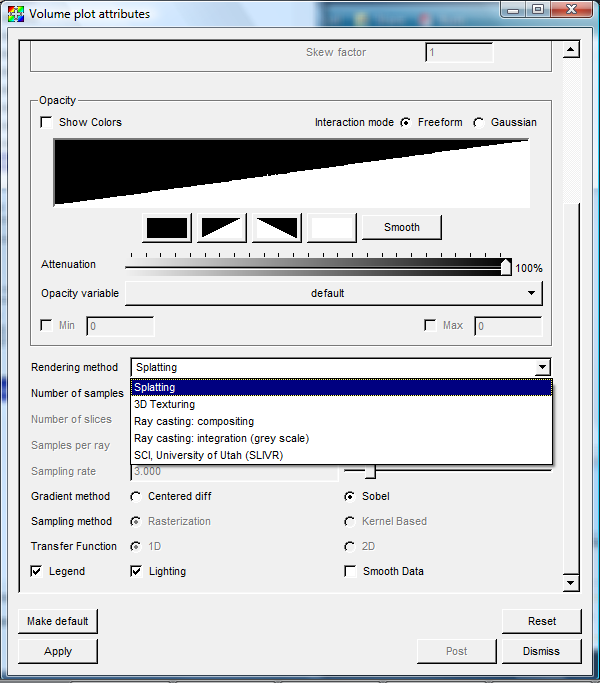
\includegraphics[width=.4\textwidth]{VisItVolumeAttributes2.png}
%   \caption{Volume visualization attributes window}
%   \label{VisItVolumeAttributes2}
% \end{wrapfigure}
\end{enumerate}


\begin{figure}[h]
  \centering
  \vspace{-10pt}
  \subfloat[Visualization of a volume on the viewer window]{\label{VisItVolumeTempINATK08Viewer}
  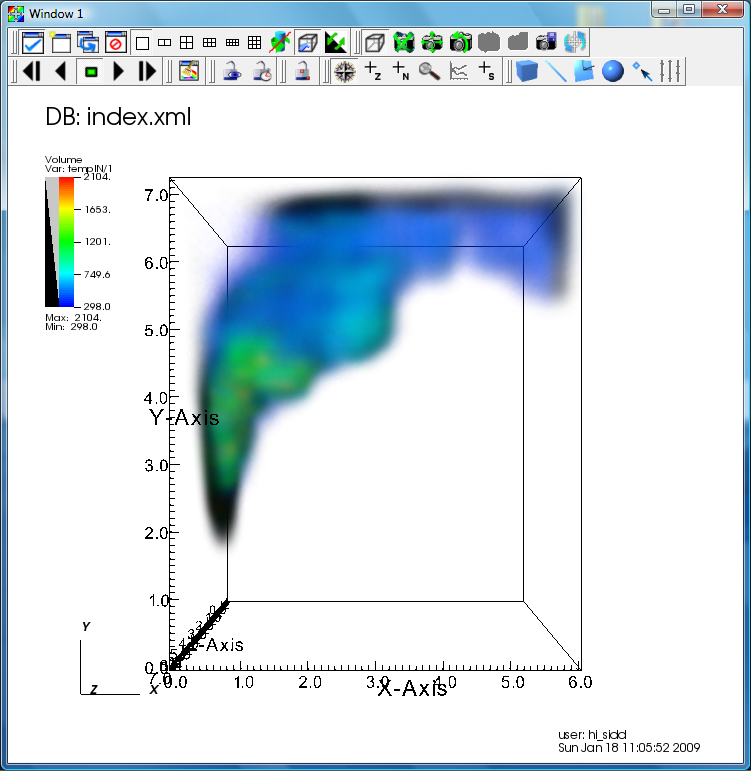
\includegraphics[width=.3\textwidth]{VisItVolumeTempINATK08Viewer.png}}
  \hspace{10pt}
  \subfloat[Volume visualization attributes window]{\label{VisItVolumeAttributes1}
  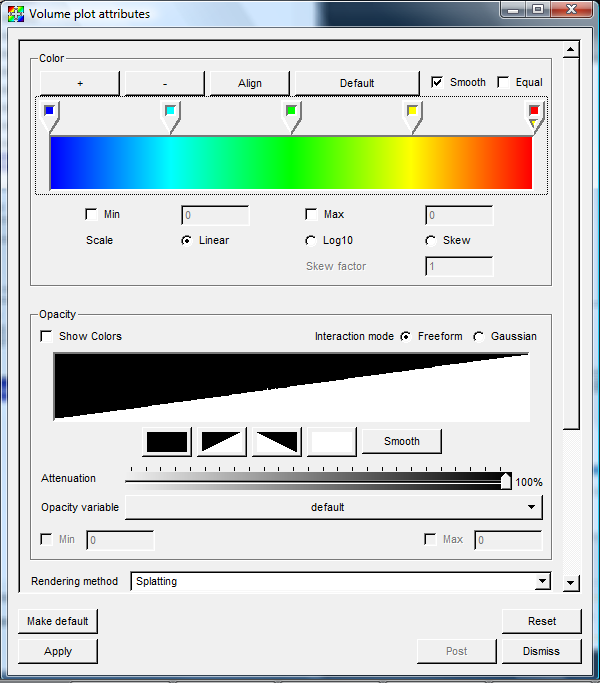
\includegraphics[width=.3\textwidth]{VisItVolumeAttributes1.png}}
  \hspace{10pt}
  \subfloat[Volume visualization attributes window]{\label{VisItVolumeAttributes2}
  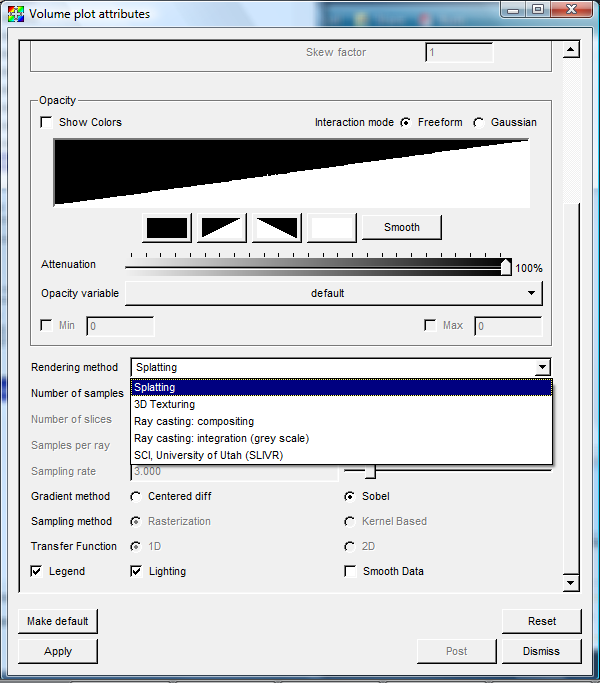
\includegraphics[width=.3\textwidth]{VisItVolumeAttributes2.png}}
  \caption{}
  \vspace{-10pt}
  \label{}
\end{figure}

The tab Color specifies the color table and the various options
associated with it. The user can add/ remove control points by
clicking on the + and - buttons. These can then be equally spaced by
pressing the Align button.

A different color table can be selected by clicking on the Default
button and then selecting an appropriate color table. The color(s)
associated with the control points can be changed by right-clicking on
the them and then selecting an appropriate color.

The user also has the option of specifying a Min and Max on the scalar
value range by checking on the associated box(s) and entering in the
values.

\begin{wrapfigure}{r}{.5\textwidth}
  \center
  \vspace{-20pt}
  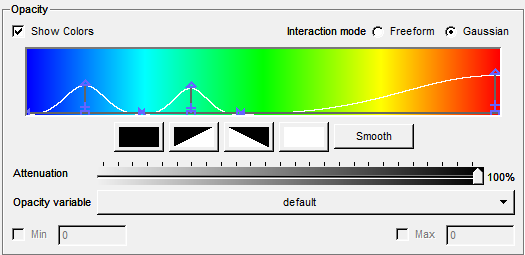
\includegraphics[width=.4\textwidth]{VisItTransferFunction.png}
  \caption{The opacity transfer function in the attributes window}
  \label{VisItTransferFunction}
\end{wrapfigure}

The second tab Opacity lets you specify a transfer function for the
color table. Clicking on the check box Show Colors copies the colors
from the color table onto this graph. Selecting the Interaction Mode
as Gaussian lets you draw curves and specify a more accurate color
table (Figure~\ref{VisItTransferFunction}).

You can add in as many curves on the graph by clicking on the left
mouse button and then placing them accordingly. To delete an unwanted
curve, just right click on it.

After specifying an opacity transfer function, one can select an
appropriate rendering method, Splatting being the default. The related
fields thereafter become active/ inactive as and when different
rendering methods are selected.

\subsection{Particle visualization}

\begin{enumerate}

\item To add particles, we select the Molecule plot and then click on
  the variable p.temperature as shown in the
  Figure~\ref{VisItMoleculePTempATK08}. The asterisk '*' refers to all
  the materials associated with the variable.

% \begin{wrapfigure}{r}{.5\textwidth}
%   \center
%   \vspace{-30pt}
%   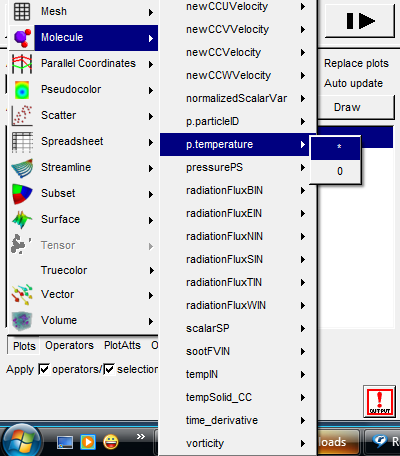
\includegraphics[width=.4\textwidth]{VisItMoleculePTempATK08.png}
%   \caption{Selecting a molecule plot and an associated variable/ material}
%   \label{VisItMoleculePTempATK08}
% \end{wrapfigure}

\item The variable p.temperature/* now appears on the Active plots
  list. Select the variable and hit Draw. A container in the form of
  particles now appears on the Viewer window.

\item Now double click on the variable name in Active plots list. This
  brings up the Molecule plot attributes window as shown in
  Figure~\ref{VisItMoleculeAttributesPTemp1}.

\end{enumerate}


\begin{figure}[h]
  \centering
  \vspace{-10pt}
 \subfloat[Selecting a molecule plot and an associated variable/ material]{\label{VisItMoleculePTempATK08}
 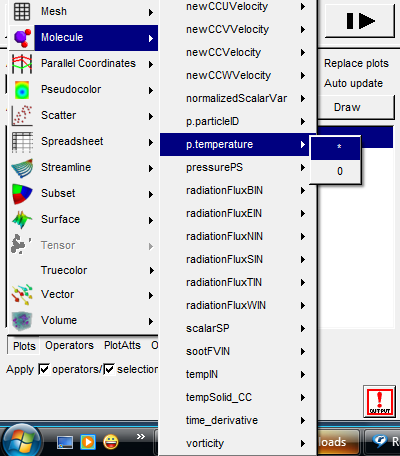
\includegraphics[width=.3\textwidth]{VisItMoleculePTempATK08.png}}
  \hspace{10pt}
 \subfloat[Selecting a molecule plot and an associated variable/ material]{\label{VisItMoleculeAttributesPTemp1}
 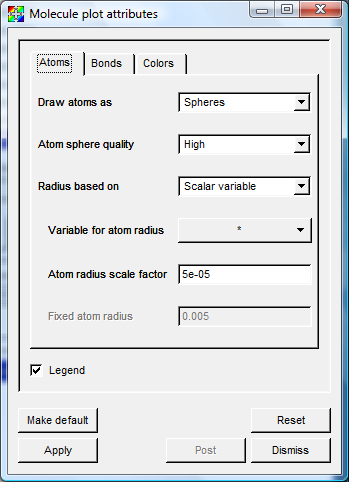
\includegraphics[width=.3\textwidth]{VisItMoleculeAttributesPTemp1.png}}
 \hspace{10pt}
 \subfloat[Selecting a molecule plot and an associated variable/ material]{\label{VisItMoleculePTtempViewer}
 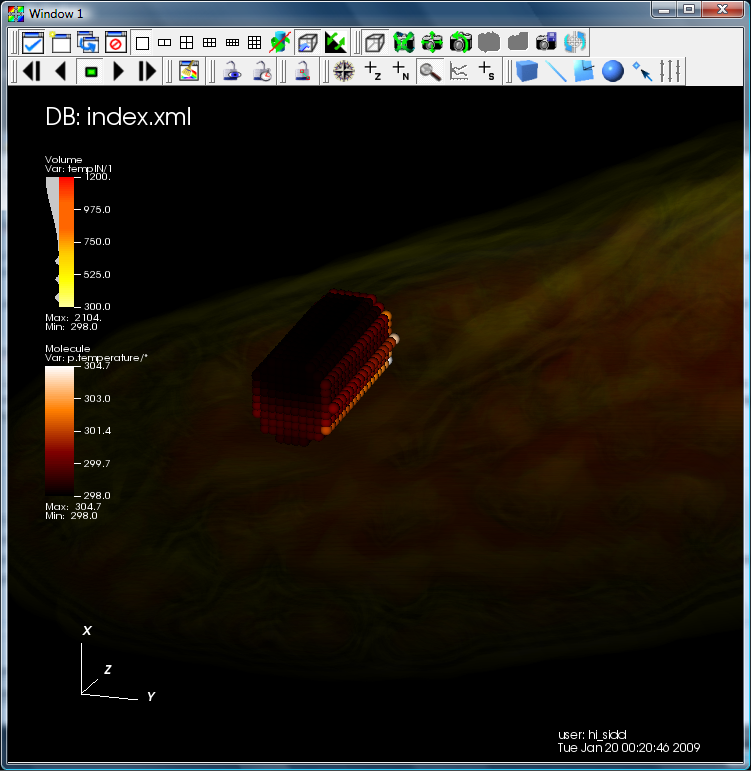
\includegraphics[width=.3\textwidth]{VisItMoleculePTtempViewer.png}}
 \vspace{-10pt}
  \caption{}
  \label{}
\end{figure}


% \begin{wrapfigure}{r}{.5\textwidth}
%   \center
%   \vspace{-30pt}
%   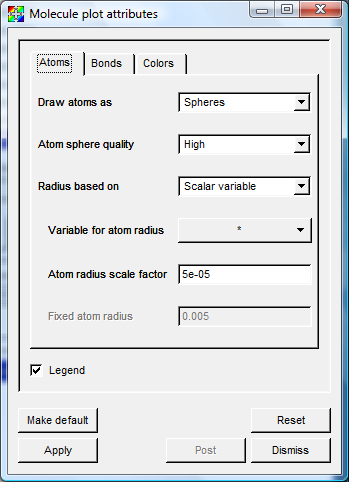
\includegraphics[width=.4\textwidth]{VisItMoleculeAttributesPTemp1.png}
%   \caption{Selecting a molecule plot and an associated variable/ material}
%   \label{VisItMoleculeAttributesPTemp1}
% \end{wrapfigure}

We choose to visualize the particles as Sphere Impostors (doesn't runs
the GPU out of memory, drawing as Spheres does). We also choose to
scale the sphere radius by a Scalar Variable and specify that variable
to be p.temperature/* itself (therefore the * appears). Since the
temperature values are too high, we scale them all by a factor of
5.e-05 (on the basis of trial and error). Finally in Colors tab, we
set the Color map for scalars as orangehot.  Combined with volume
visualization, we get a visualization as shown in
Figure~\ref{VisItMoleculePTtempViewer}.

% \begin{wrapfigure}{r}{100mm}
%   \center
%   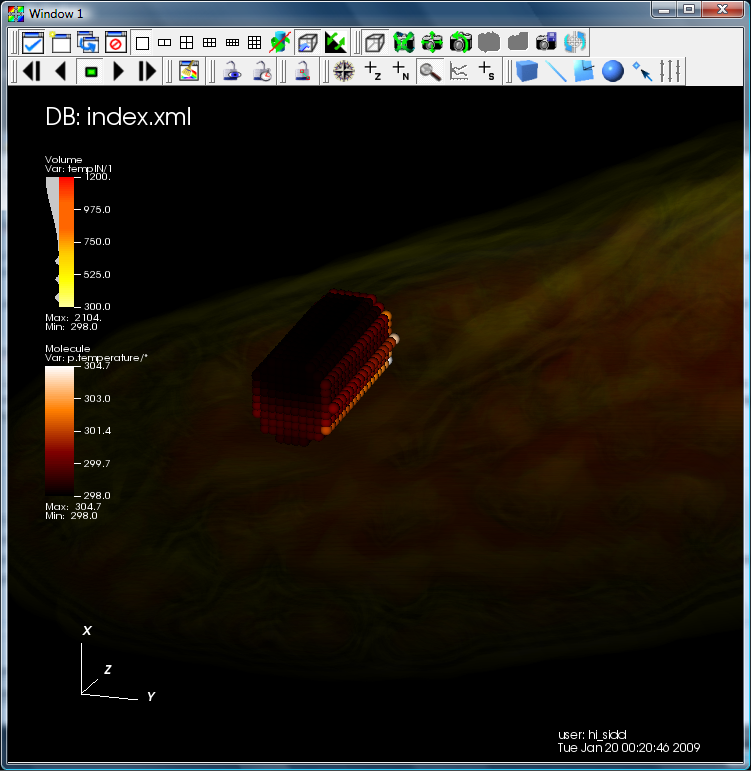
\includegraphics[width=.5\linewidth]{VisItMoleculePTtempViewer.png}
%   \caption{Selecting a molecule plot and an associated variable/ material}
%   \label{VisItMoleculePTtempViewer}
% \end{wrapfigure}

\subsection{Visualizing patch boundaries}
% In order to generate an image, like the one shown in
% Figure~\ref{VisItSubsetPlot}, we use the Subset plot. As with other
% variables, we select the Subset plot and an associated variable. The
% variables have a prefix 'level/ patch'. There is a level/ patch
% variable associated with every kind of variable (Cell Centered, Node
% Centered, Face Centeerd) present in the dataset. In the
% figure~\ref{VisItSubsetPlotVariables}, we select one such variable.
In order to visualize patch boundaries, we use the Subset plot. As
with other variables, we select the Subset plot and an associated
variable. The variables have a prefix 'level/ patch'. There is a
level/ patch variable associated with every kind of variable (Cell
Centered, Node Centered, Face Centered) present in the dataset. In the
Figure~\ref{VisItSubsetPlotVariables}, we select one such variable.
Next, we hit Draw. This produces a visualization as shown in
Figure~\ref{VisItSubsetPlotViewer}.

%\begin{figure}
%  \center
%  \includegraphics[scale=0.5]{VisItSubsetPlot.png}
%  \caption{Visualizing patch boundaries}
%  \label{VisItSubsetPlot}
%\end{figure}

% \begin{wrapfigure}{r}{.5\textwidth}
%   \center
%   \includegraphics[width=.4\textwidth]{VisItSubsetPlotVariables.png}
%   \caption{A patch/ level variable, associated with every kind of variable}
%   \label{VisItSubsetPlotVariables}
% \end{wrapfigure}

\begin{figure}[h]
  \centering
 \subfloat[A patch/ level variable, associated with every kind of variable]{\label{VisItSubsetPlotVariables}
  \includegraphics[width=.3\textwidth]{VisItSubsetPlotVariables.png}}
  \hspace{50pt}
 \subfloat[The default visualization of patches]{\label{VisItSubsetPlotViewer}
 \includegraphics[width=.3\textwidth]{VisItSubsetPlotViewer.png}}
 \vspace{-20pt}
  \caption{}
  \label{}
\end{figure}



To generate a wire-frame model, we double click on the Subset plot in
the Active plots window. This pops up the Subset plot attributes
window, where we check the Wireframe mode as shown in
Figure`\ref{VisItSubsetPlotAttrib}. This would produce a
visualization, similar to one shown in
Figure~\ref{VisItSubsetPlotWireframe}.

% \begin{wrapfigure}{r}{.5\textwidth}
%   \center
%   \includegraphics[width=.4\textwidth]{VisItSubsetPlotViewer.png}
%   \caption{The default visualization of patches}
%   \label{VisItSubsetPlotViewer}
% \end{wrapfigure}

% \begin{wrapfigure}{r}{100mm}
%   \center
%   \includegraphics[width=.5\linewidth]{VisItSubsetPlotAttrib.png}
%   \caption{Enabling the 'Wireframe' mode for visualizing patch boundaries}
%   \label{VisItSubsetPlotAttrib}
% \end{wrapfigure}

% \begin{wrapfigure}{r}{100mm}
%   \center
%   \includegraphics[width=.5\linewidth]{VisItSubsetPlotWireframe.png}
%   \caption{The patch boundaries after enabling the wireframe mode}
%   \label{VisItSubsetPlotWireframe}
% \end{wrapfigure}

\begin{figure}[h]
  \centering
 \vspace{-5pt}
 \subfloat[Enabling the 'Wireframe' mode for visualizing patch boundaries]{\label{VisItSubsetPlotAttrib}
  \includegraphics[width=.25\textwidth]{VisItSubsetPlotAttrib.png}}
  \hspace{50pt}
 \subfloat[The patch boundaries after enabling the wireframe mode]{\label{VisItSubsetPlotWireframe}
 \includegraphics[width=.3\textwidth]{VisItSubsetPlotWireframe.png}}
 \vspace{-10pt}
  \caption{}
 \vspace{-10pt}
  \label{}
\end{figure}

\subsection{Iso-surfaces}

The easiest way to draw iso-surfaces is to use the 'Contour' Plot. As
with other plots demonstrated above, the contour plot is selected on a
regular 3D scalar variable. Figure ~\ref{VisItContourPlot} illustrates
this.

\begin{wrapfigure}{r}{.5\textwidth}
  \center
  \vspace{-35pt}
  \includegraphics[width=0.4\textwidth]{VisItContourPlot.png}
  \caption{Selecting the 'Contour' plot on a regular 3D scalar variable}
  \label{VisItContourPlot}
\end{wrapfigure}

Once the plot is selected, we hit 'Draw'. This would produce a
visualization, similar to one shown in
Figure~\ref{VisItContourPlotViewer}. You can then modify the plot
attributes by double clicking on the plot in the 'Active plots'
window. This would pop up the 'Contour plot attributes window', as
shown in Figure~\ref{VisItContourPlotAttrib}.

The 'Select by' option can be changed to 'Value(s)' and
'Percent(s)'. When specifying multiple values, they should be
separated by a space.


% \begin{wrapfigure}{r}{100mm}
%   \center
%   \includegraphics[scale=0.25]{VisItContourPlotViewer.png}
%   \caption{Iso-surface visualization}
%   \label{VisItContourPlotViewer}
% \end{wrapfigure}

% \begin{wrapfigure}{r}{100mm}
%   \center
%   \includegraphics[scale=0.5]{VisItContourPlotAttrib.png}
%   \caption{The attributes window for the 'Contour' plot}
%   \label{VisItContourPlotAttrib}
% \end{wrapfigure}

\begin{figure}[h]
  \centering
 \vspace{5pt}
 \subfloat[Iso-surface visualization]{\label{VisItContourPlotViewer}
  \includegraphics[width=.5\textwidth]{VisItContourPlotViewer.png}}
  \hspace{50pt}
 \subfloat[The attributes window for the 'Contour' plot]{\label{VisItContourPlotAttrib}
 \includegraphics[width=.25\textwidth]{VisItContourPlotAttrib.png}}
 \vspace{-10pt}
  \caption{}
 \vspace{-10pt}
  \label{}

\end{figure}


\subsection{Streamlines}

The 'Streamlines' plot has issues with the current version of VisIt
(1.11.2 and older). However, these have been corrected in the trunk
and should be out in version 2.0. The controls remain the same in all
these version and the example below was implemented on the trunk
version.

As shown in Figure~\ref{VisItStreamlinesPlot} we select the
'Streamlines' plot on a vector variable. We then double click on the
plot itself, which pops up the 'Streamlines attributes window'.

\begin{wrapfigure}{r}{.5\textwidth}
  \center
  \vspace{-10pt}
  \includegraphics[width=.4\textwidth]{VisItStreamlinesPlot.png}
  \caption{Selecting the 'Streamlines' plot on a vector variable}
  \label{VisItStreamlinesPlot}
\end{wrapfigure}

We set the 'Distance' parameter such that it covers the entire
computational domain. We set the 'Streamline direction' as forward. In
the 'Source' tab, Figure~\ref{VisItStreamlinesAttrib1}, we define the
'Source type' as 'Line'. We can select other options too, notably
'Single Point', 'Sphere' etc. We now define the line 'Start' and 'End'
coordinates. In this specific case, we define them as [-0.1 -0.05 0]
and [-0.1 0.05 0] respectively. This choice ensures that we cover the
entire y axis and start at the leftmost corner of the computational
domain.

To ensure that our stream lines are smooth, we change the 'Maximum
step length' in the in the 'Advanced' tab. In this case, we change it
to 1.e-05. The thing to keep in mind is that this length should be
order of magnitude smaller than the length of the computational
domain. This is shown in Figure ~\ref{VisItStreamlinesAttrib2}.

% \begin{wrapfigure}{r}{.5\textwidth}
%   \center
%   \includegraphics[width=.4\textwidth]{VisItStreamlinesAttrib1.png}
%   \caption{Setting the 'Source' tab parameters}
%   \label{VisItStreamlinesAttrib1}
% \end{wrapfigure}

% \begin{wrapfigure}{r}{.5\textwidth}
%   \center
%   \includegraphics[width=.4\textwidth]{VisItStreamlinesAttrib2.png}
%   \caption{Setting the 'Advanced' tab parameters}
%   \label{VisItStreamlinesAttrib2}
% \end{wrapfigure}

Once these parameters are set, we hit 'Apply' and then click on the 'Draw' button on the gui. This produces a visualization similar to one shown in Figure ~\ref{VisItStreamlinesViewer}.

% \begin{wrapfigure}{r}{100mm}
%   \center
%   \includegraphics[scale=0.4]{VisItStreamlinesViewer.png}
%   \caption{Streamlines visualization}
%   \label{VisItStreamlinesViewer}
% \end{wrapfigure}


\begin{figure}[h]
  \centering
 \vspace{5pt}
 \subfloat[Setting the 'Source' tab parameters]{\label{VisItStreamlinesAttrib1}
  \includegraphics[width=.25\textwidth]{VisItStreamlinesAttrib1.png}}
  \hspace{10pt}
 \subfloat[Setting the 'Advanced' tab parameters]{\label{VisItStreamlinesAttrib2}
 \includegraphics[width=.25\textwidth]{VisItStreamlinesAttrib2.png}}
 \hspace{10pt}
 \subfloat[Streamlines visualization]{\label{VisItStreamlinesViewer}
 \includegraphics[width=.4\textwidth]{VisItStreamlinesViewer.png}}
  \caption{}
 \vspace{-10pt}
  \label{}
\end{figure}


\subsection{Visualizing extra cells}

For visualizing extra cells we use the 'Inverse Ghost Zone' operator
~\ref{VisItInverseGhostZoneOp} in conjunction with the 'Pseudocolor'
plot. Since the plugin reads in extra cells as ghost cells, the usage
of this operator make sense in this scenario.

% \begin{wrapfigure}{r}{.5\textwidth}
%   \center
%   \vspace{-20pt}
%   \includegraphics[width=0.15\textwidth]{VisItInverseGhostZoneOp.png}
%   \caption{Selecting the Inverse Ghost Zone operator}
%   \label{VisItInverseGhostZoneOp}
% \end{wrapfigure}

After the operator is applied to the 'Pseudocolor' plot, we double
click on the operator to change its attributes. We switch to 'Both
ghost zones and real zones' in this window
~\ref{VisItInverseGhostZoneAttribs} and hit 'Apply'.

% \begin{wrapfigure}{r}{.5\textwidth}
%   \center
%   \includegraphics[width=0.4\textwidth]{VisItInverseGhostZoneAttribs.png}
%   \caption{The attributes window for the 'Inverse Ghost Zone' operator}
%   \label{VisItInverseGhostZoneAttribs}
% \end{wrapfigure}

We then hit 'Draw'. When combined with the 'Mesh' plot we get a visualization similar to the one shown in Figure ~\ref{VisItInverseGhostZoneViewer}. The pick operations on the viewer can then be used to investigate the value(s) in these extra cells.

% \begin{wrapfigure}{r}{.5\textwidth}
%   \center
%   \includegraphics[width=0.4\textwidth]{VisItInverseGhostZoneViewer.png}
%   \caption{Extra cells together with the 'Mesh' plot}
%   \label{VisItInverseGhostZoneViewer}
% \end{wrapfigure}

\begin{figure}[h]
  \centering
 \vspace{5pt}
 \subfloat[Selecting the Inverse Ghost Zone operator]{\label{VisItInverseGhostZoneOp}
  \includegraphics[width=.15\textwidth]{VisItInverseGhostZoneOp.png}}
  \hspace{20pt}
 \subfloat[The attributes window for the 'Inverse Ghost Zone' operator]{\label{VisItInverseGhostZoneAttribs}
 \includegraphics[width=.25\textwidth]{VisItInverseGhostZoneAttribs.png}}
 \hspace{20pt}
 \subfloat[Extra cells together with the 'Mesh' plot]{\label{VisItInverseGhostZoneViewer}
 \includegraphics[width=.45\textwidth]{VisItInverseGhostZoneViewer.png}}
  \caption{}
 \vspace{-10pt}
  \label{}
\end{figure}


\subsection{Picking on particles}

The 'Node pick mode' on the visualization window can be used to pick
particles and investigate particles attributes. After plotting
particles using the 'Molecule' plot, the user can then select the
'Node pick mode' ~\ref{VisItNodePick} and select particles (by
clicking on them) of interest.

 \begin{wrapfigure}{r}{.5\textwidth}
   \center
   \includegraphics[width=0.5\textwidth]{VisItNodePick.png}
   \caption{The 'Node pick mode' on the visualization window}
   \label{VisItNodePick}
 \end{wrapfigure}

Once a particle is picked, the 'Pick' window pops up with the particle
attributes. By default only the variable plotted is queried, if the
user wants to query more variables per pick - they can be added by
selecting additional variables from the 'Variables' menu and as shown
in the Figure ~\ref{VisItPickWindow}.

% \begin{wrapfigure}{r}{.5\textwidth}
%   \center
%   \includegraphics[width=0.4\textwidth]{VisItPickWindow.png}
%   \caption{The 'Pick' window }
%   \label{VisItPickWindow}
% \end{wrapfigure}

% \begin{figure}[h]
%   \centering
%  \vspace{5pt}
%  \subfloat[The 'Node pick mode' on the visualization window]{\label{VisItNodePick}
%   \includegraphics[width=.4\textwidth]{VisItNodePick.png}}
%   \hspace{20pt}
%  \subfloat[The 'Pick' window]{\label{VisItPickWindow}
%  \includegraphics[width=.4\textwidth]{VisItPickWindow.png}}
%   \caption{}
%  \vspace{-10pt}
%   \label{}
% \end{figure}

\begin{figure}[h]
  \centering
  \includegraphics[width=.4\textwidth]{VisItPickWindow.png}
  \caption{The 'Pick' window}
  \label{VisItPickWindow}
\end{figure}

\subsection{Selectively visualizing vectors}
The expression editor can be used to define a vector variable with magnitude greater or lesser than a certain extent. An example of this is shown below,

\begin{verbatim}
if(gt(magnitude(<vel_CC/1>), 0.0), <vel_CC/1>, {0, 0, 0})
\end{verbatim}

Put into words, if magnitude of vel\_CC/1 is greater than 0.0, display it, else display a zero magnitude vector. To use the 'lesser than' parameter, replace 'gt' with 'lt'.

%\section{Python CLI and VisIt}
%Aside from the normal GUI, VisIt also presents options for CLI (Command Line Interface) %manipulation. The CLI of VisIt is very useful and can generate images without ever %opening any VisIt window. Thus saving substantial time and computation for large %visualizations. There is a simple example cis
%\chapter{Visualization Tools -- Manta}

%To run the C-SAFE scene:
%\begin{Verbatim}[fontsize=\footnotesize]
%  Manta/build/bin/csafe_scene
%\end{Verbatim}

%The csafescene window will open showing a transfer function editor.  To add files to load run:
%\begin{Verbatim}[fontsize=\footnotesize]
%  File -> Add/Remove NRRD Files
%\end{Verbatim}

%\begin{figure}[htbp]
%  \center
%  \includegraphics[width=.5\linewidth]{manta_files.png}
%  \caption{Opening the scene}
%  \label{fig:manta_files}
%\end{figure}

% This will open a window where you can add volume and particle files in .nrrd or .nhdr formats.  Select add particle file(s) and open a particle nrrd file in .nhdr or .nrrd format.  These nrrd files should be created with the uda2nrrd tool.

% \begin{figure}[htbp]
%   \center
%   \includegraphics[width=.5\linewidth]{manta_add_files.png}
%   \caption{Adding files to the scene}
%   \label{fig:manta_add_files}
% \end{figure}

% A similarly named volume nrrd should be automatically added if in the same folder.  Close the window by pressing "OK".  The files won't be loaded yet so you can make modifications to the data to be loaded in before loading them.  To load the files:

% \begin{Verbatim}[fontsize=\footnotesize]
%   Scene -> Generate
% \end{Verbatim}

% The resulting csafe scene window should look similar to:

% \begin{figure}[htbp]
%   \center
%   \includegraphics[width=.5\linewidth]{manta_histograms.png}
%   \caption{C-SAFE window with histograms from loaded nrrd files}
%   \label{fig:manta_histograms}
% \end{figure}

% and a separate window will open showing the visualization.

% \section{Manta Commandline options}
% Many of the operations typically used through the GUI can be used through the commandline when running the csafe scene.

% \begin{enumerate}

% \item
% --np=<int>  : the number of processes to devote to Manta. Should be roughly equivalent to the number of cores in your system.
% \item
% --cfg=<string>  : load a configuration file, this has histogram and filenames saved
% \item
% --nrrdlist=<string>  : load a nrrdlist
% \item
% --uda=<string>  : load an UDA file
% \item
% --res <int>x<int>: resolution of window, ie 512x512
% \item
% --g  : generate (load) all datasets when starting up, should be used in conjunction with --nrrdlist or --cfg

% \end{enumerate}

% Additionally, many of the commandline options that Manta uses can also be used with the csafe scene.  These commands configure rendering options.  For example, jittered sampling may reduce aliasing effects.

% \begin{enumerate}

% \item
% --imagetype <string> : manta image type (see manta command line options)
% \item
% --shadows <string> : manta shadow algorithm (see manta command line options)
% \item
% --imagetraverser <string> : manta image traverser (see manta command line options)
% \item
% --loadbalancer <string> : manta load balancer option (see manta command line options)
% \item
% --renderer <string> : manta renderer (see manta command line options)


% \end{enumerate}

% \section{Saving and Loading}

% You can save the status of your project through File->Save or File->save as. Note that saving your project saves everything from the clipping regions to the transfer functions but currently does not save some things such as the background color or the camera position.

% Exporting transfer functions: You can export the transfer function currently displayed by selecting File->Export Transfer Function. This is The exported format is as follows: position r g b a position r g b a ... position is a number (0-1) that specifies the position of your control point in the transfer function. r g b a are simply the color and alpha values of the control point.

% You can import saved transfer functions from File->import Transfer Function.

% The configuration file saves the data files used however if you would like to use the same configuration file for multiple sets of data you can select File->Export NrrdList.  This stores the data files as a list in ASCII which can be imported to use with any configuration.

% \section{Using the Transfer Function Editor}

% \begin{figure}[htbp]
%   \center
%   \includegraphics[width=.5\linewidth]{transferF.png}
%   \caption{Transfer function editor.}
%   \label{fig:manta_tf}
% \end{figure}

% The transfer function display in the histogram window displays the currently selected transfer function. To select a different transfer function, click on the color wheel icon next to the histogram. The transfer function can be modified in a similar fashion to gradient editors in popular image editing programs. The color and opacity of the data range can be adjusted by modifying the control points. The default transfer function is a rainbow. To change a color, select a control point and click the color wheel to edit it. Or you can simply right-click on a control point to change the color. To modify opacity, simply move the control points up and down by clicking and dragging them.

% \section{Histogram Controls}

% \begin{figure}[htbp]
%   \center
%   \includegraphics[width=.5\linewidth]{histogram.png}
%   \caption{Histogram with controls.}
%   \label{fig:manta_histogram}
% \end{figure}

% Histograms represent the frequency of data values in a data set. Each histogram is associated with an index into either a volume or sphere data. If you select index 0 in the sphere data set, then the histogram mostly likely shows the accumulated range of x-coordinates for all of the sphere data sets. There is a semi-transparent grey box overlaying each histogram. This represents the range of values in the histogram that are displayed. Clicking on the right or left side of this box moves the left or right side of the clipping region accordingly. You can also click and drag the middle of the region to drag the region along the histogram. You can also use the mouse wheel to zoom into a region of the histogram.
%   Name (\#) - The name associated with the histogram and the index it corresponds to in the NRRD file.
% To the right are various controls.

% \begin{enumerate}
% \item
% colorwheel : This will make this histogram's transfer function display in the transfer function panel and also make it the active transfer function for either the volume or sphere data.
% \item
% Ruler : you can explicitly set specific data ranges for the clipping region or the region of the data to which the transfer function applies to. This is extremely useful if there is only a vary narrow region of the data range that you want to be looking at.
% \item
% Zoom in/out: this will zoom in to the clipping region or back out to the zoom where you were previously.
% \end{enumerate}

% \section{Ambient Occlusion}
%   Ambient occlusion is an approximation of global illumination and can give a better sense of relative depth in clusters of objects.  To enable ambient occlusion turn it on in Scene->Preferences.  There are two variables to modify, the cutoff distance and the number of rays shot.  The cutoff distance is how far away objects can be to occlude rays.  To produce a good image it is a good idea to turn off the volume and reduce or remove the lights.  The light can be turned off in the Light dialog in the Manta Menu.  Setting the light color to black will completely disable a light.

% %\section{CSAFE Window Menus}

% % \subsection{File - Save and Load Configuration File}

% % \subsection{File - Save and Load NRRDFile}

% % \subsection{File - Add Remove NRRD Files}

% % \subsection{File - Import Export Transfer Function}

% % \subsection{Scene - Add Histogram}

% % \subsection{Scene - Scene Preferences}

% % \subsection{Scene - Volume Position Size}

% % \subsection{Scene - Cutting Bounding Box}

% % \subsection{Scene - Generate}

% % \section{Manta Window Menus}

% % \subsection{File - Threads}

% % \subsection{Camera - Auto View}

% % \subsection{Camera - Edit Camera}

% % \subsection{Camera - Edit Background}

% % \subsection{Camera - Camera Paths}

% % \subsection{Camera - Capture Frames}

% % \subsection{Lights - Edit Lights}

% % \subsection{Lights - Enable Visible Lights}


% \section{Manta FAQ}

% \begin{enumerate}
% \item
% Q. "I get an error Gtk-CRITICAL **: file gtkrange.c".
% A.  This error pops up on some system and can safely be ignored.
% Q.  "It is running very slowly"
% A.  Try increasing the number of threads, shrinking the window size, and reducing the step size through the volume.
% \end{enumerate}


%__________________________________
\chapter{Data Extraction Tools}

Uintah offers a number of tools for accessing data stored in Uintah
Data Archives (``UDAs").  Because the format of Uintah data is
specific to the framework, these tools allow a user to quickly extract
data, which can then either be postprocessed within that tool (simple
modification of the source code may be necessary), postprocessed with
external software such as Matlab or Octave, or simply plotted with,
e.g. gnuplot.  These tools are not compiled automatically when ``make
sus'' is issued.  To compile them cd to ``opt/StandAlone/tools'' and
issue ``make''.  These tools are described below.

\section{puda}

The command line extraction utility \tt puda \normalfont (for ``parse
Uintah data archive") has a number of uses.  For example, it may be
used to extract a subset of particle data from a UDA.  Once the
extraction tools have been compiled, the puda executable will be
located in \tt opt/StandAlone/tools/puda/. \normalfont If the
executable is run with no additional command line arguments, the
following usage information will be displayed:

\begin{Verbatim}[fontsize=\footnotesize]
Usage: puda [options] <archive file>

Valid options are:
  -h[elp]
  -timesteps
  -gridstats
  -listvariables
  -varsummary
  -jim1
  -jim2
  -partvar <variable name>
  -asci
  -tecplot <variable name>
  -no_extra_cells     (Excludes extra cells when iterating over cells.
                       Default is to include extra cells.)
  -cell_stresses
  -rtdata <output directory>
  -PTvar
  -ptonly             (prints out only the point location
  -patch              (outputs patch id with data)
  -material           (outputs material number with data)
  -NCvar <double | float | point | vector>
  -CCvar <double | float | point | vector>
  -verbose            (prints status of output)
  -timesteplow <int>  (only outputs timestep from int)
  -timestephigh <int> (only outputs timesteps up to int)
  -matl,mat <int>         (only outputs data for matl)
*NOTE* to use -PTvar or -NVvar -rtdata must be used
*NOTE* ptonly, patch, material, timesteplow, timestephigh are used in conjunction with -PTvar.
\end{Verbatim}

As an example of how to use \tt puda, \normalfont suppose that one
wanted to know the locations of all particles at the last archived
timestep for the \tt const\_test\_hypo.uda \normalfont First one may
wish to know how many timesteps have been archived.  This could be
accomplished by:

\begin{Verbatim}[fontsize=\footnotesize]
 puda -timesteps const_test_hypo.uda
\end{Verbatim}
The resulting terminal output would be:
\begin{Verbatim}[fontsize=\footnotesize]
Parsing const_test_hypo.uda/index.xml
There are 11 timesteps:
1: 1.8257001926347728e-05
548: 1.0012914931998474e-02
1094: 2.0005930425875382e-02
1640: 3.0015616802173569e-02
2184: 4.0005272397960444e-02
2728: 5.0011587657447343e-02
3271: 6.0016178181543284e-02
3812: 7.0000536667661845e-02
4353: 8.0001537138146825e-02
4893: 9.0000702723306208e-02
5433: 1.0001655973087024e-01
\end{Verbatim}

These represent all of the timesteps for which data has been archived.
Suppose now that we wish to know what the stress state is for all
particles (in this case two) at the final archived timestep.  For this
one could issue:

\begin{Verbatim}[fontsize=\footnotesize]
puda -partvar p.stress -timesteplow 10 -timestephigh 10 const_test_hypo.uda
\end{Verbatim}

The resulting output is:

\begin{Verbatim}[fontsize=\footnotesize]
Parsing const_test_hypo.uda/index.xml
1.00016560e-01 1 0 281474976710656 -2.72031498e-10 -1.05064208e-26 -2.53781271e-08 -1.05064208e-26 -2.72031498e-10 -1.23584688e-09 -2.53781271e-08 -1.23584688e-09 1.63840079e-07
1.00016560e-01 1 1 0 1.93256890e-13 6.56787331e-18 1.85514400e-14 6.56787331e-18 2.24310469e-13 1.85519650e-14 1.85514400e-14 1.85519650e-14 -3.20052991e+06
\end{Verbatim}

The first column is the simulation time, the third column is the
material number, the fourth column is the particle ID, and the
remaining nine columns represent the components of the Cauchy stress
tensor ($ \sigma_{11}$,$\sigma_{12}$,$\sigma_{13}$, ...,
$\sigma_{32}$,$\sigma_{33}$).  If desired, the terminal output can be
redirected to a text file for further use.

\section{partextract}

The command-line utility \tt partextract \normalfont may be used to
extract data from an individual particle.  To do this you first need
to know the ID number of the particle you are interested in.  This may
be done by using the puda utility, or the visualization tools.  Once
the extraction tools have been compiled, the partextract utility
executable will be located in \tt /opt/StandAlone/tools/extractors/
\normalfont.  If the executable is run without any arguments the
following usage guide will be displayed in the terminal:

\begin{Verbatim}[fontsize=\footnotesize]
No archive file specified
Usage: partextract [options] <archive file>

Valid options are:
  -mat <material id>
  -partvar <variable name>
  -partid <particleid>
  -part_stress [avg or equiv or all]
  -part_strain [avg/true/equiv/all/lagrangian/eulerian]
  -timesteplow [int] (only outputs timestep from int)
  -timestephigh [int] (only outputs timesteps upto int)
\end{Verbatim}

As an example of how to use the partextract utility, suppose we wanted
to find the velocity at every archived timestep for the particle with
ID 281474976710656 (found above using puda) in the
``const\_test\_hypo.uda'' file (src/StandAlone/inputs/MPM).  The
appropriate command to issue is:

\begin{Verbatim}[fontsize=\footnotesize]
partextract -partvar p.velocity -partid 281474976710656 const\_test\_hypo.uda
\end{Verbatim}

The output to the terminal is:

\begin{Verbatim}[fontsize=\footnotesize]
Parsing const_test_hypo.uda/index.xml
1.82570019e-05 1 0 281474976710656 0.00000000e+00 0.00000000e+00 -1.00000000e-02
1.00129149e-02 1 0 281474976710656 -1.03554318e-19 -1.03554318e-19 -1.00000000e-02
2.00059304e-02 1 0 281474976710656 -1.99388121e-19 -1.99388121e-19 -1.00000000e-02
	.
	.
	.
\end{Verbatim}

It is noted that if the stress tensor is output using the partextract utility, the output format is different than for the puda utility.  The partextract utility only outputs the six independent components instead of all nine.  For example, if we use partextract to get the stress tensor for the same particle as above at the last archived timestep only, the output is:

\begin{Verbatim}[fontsize=\footnotesize]
partextract -partvar p.stress -partid 281474976710656 -timesteplow 10 -timestephigh 10 const_test_hypo.uda
Parsing const_test_hypo.uda/index.xml
1.00016560e-01 1 0 281474976710656 -2.72031498e-10 -1.05064208e-26 -2.53781271e-08 -1.05064208e-26 -2.72031498e-10 -1.23584688e-09 -2.53781271e-08 -1.23584688e-09 1.63840079e-07
\end{Verbatim}

Compare this output with the output from puda above.  Notice that the
ordering of the six independent components of the stress tensor for
partextract are $\sigma_{11}$,$\sigma_{22}$, $\sigma_{33}$,
$\sigma_{23}$, $\sigma_{13}$ , $\sigma_{12}$.

\section{lineextract}

Lineextract is used to extract an array of data from a region of a
computational domain. Data can be extracted from a point, along a
line, or from a three dimensional region and then stored as a variable
for ease of post processing.

Usage: \begin{Verbatim}[fontsize=\footnotesize]
./lineextract [options] -uda <archive file>

Valid options are:
 -h,        --help
 -v,        --variable:      <variable name>
 -m,        --material:      <material number> [defaults to 0]
 -tlow,     --timesteplow:   [int] (sets start output timestep to int) [defaults to 0]
 -thigh,    --timestephigh:  [int] (sets end output timestep to int) [defaults to last timestep]
 -timestep, --timestep:      [int] (only outputs from timestep int) [defaults to 0]
 -istart,   --indexs:        <x> <y> <z> (cell index) [defaults to 0,0,0]
 -iend,     --indexe:        <x> <y> <z> (cell index) [defaults to 0,0,0]
 -l,        --level:         [int] (level index to query range from) [defaults to 0]
 -o,        --out:           <outputfilename> [defaults to stdout]
 -vv,       --verbose:       (prints status of output)
 -q,        --quiet:         (only print data values)
 -cellCoords:                (prints the cell centered coordinates on that level)
 --cellIndexFile:             <filename> (file that contains a list of cell indices)
                                  [int 100, 43, 0]
                                  [int 101, 43, 0]
                                  [int 102, 44, 0]
\end{Verbatim}

The following example shows the usage of lineextract for extracting
density data at the 60th computational cell in the x-direction,
spanning the width of the domain in the y-direction (0 to 1000), at
timestep, 7, (note ``timestep" actually refers to the seventh data
dump, not necessarily the seventh timestep in the simulation. The
variable containing the density data within the uda is ``rho\_CC," and
the output variable that will store the data for post processing is
``rho."
\begin{Verbatim}[fontsize=\footnotesize]
./lineextract -v rho_CC  -timestep 7 -istart 60 0 0 -iend 60 1000 0 -m 1 -o rho -uda test01.uda.000
\end{Verbatim}

%__________________________________
\section{compute\_Lnorm\_udas}
\TT{Compute\_Lnorm\_udas} computes the $L_1$, $L_2$ and $L_\infty$
norms for each variable in two udas.  This utility is useful in
monitoring how the solution differs from small changes in either the
solution tolerances, input parameters or algorithmic changes.  You can
also use it to test the domain size influence.  The norms are computed
using:
%
\begin{equation}
  d[i] = |uda_1[i] - uda_2[i]|
\end{equation}
%
\begin{equation}
  L_1 = \frac{\raise1.5pt\hbox{$\sum_i^\text{All Cells}$}d[i]}{\text{number of cells}}
\end{equation}
%
\begin{equation}
  L_2 = \sqrt{ \frac{\raise1.5pt\hbox{$\sum_i^\text{All Cells}$}d[i]^2}{\text{number of cells}} }
\end{equation}
%
\begin{equation}
  L_\infty = \text{max}(d[i])
\end{equation}
%
These norms are computed for each \TT{CC, NC, SFCX, SFCY, SFCZ}
variable, on each level for each timestep.  The output is displayed on
the screen and is placed in a directory named `Lnorm.'  The directory
structure is:
%
\begin{Verbatim}[fontsize=\footnotesize]
 Lnorm/
   -- L-0
    |-- delP_Dilatate_0
    |-- mom_L_ME_CC_0
    |-- press_CC_0
    |-- press_equil_CC_0
    |-- variable
    |-- variable
    |--etc
\end{Verbatim}
%
and in each variable file is the physical time, $L_1$, $L_2$ and $L_\infty.$  These data can be plotted using \TT{gnuplot} or another plotting program.

The command usage is
%
\begin{Verbatim}[fontsize=\footnotesize]
  compute_Lnorm_udas <uda1> <uda2>
\end{Verbatim}
%
The utility allows for \TT{udas} that have different computational
domains and different patch distributions to be compared.  The uda
with the smallest computational domain should always be specified
first.
%
In order for the norms to be computed the physical times must satisfy
\begin{equation*}
| \text{physical Time}_{uda_1} - \text{physical Time}_{uda_2}| < 1e^{-5}.
\end{equation*}

%__________________________________
\section{timeextract}

Timeextract is used to extract a user specified variable from a point in a computational
domain.

Usage: \begin{Verbatim}[fontsize=\footnotesize]
./timeextract [options] -uda <archive file>

Valid options are:
  -h,--help
  -v,--variable <variable name>
  -m,--material <material number> [defaults to 0]
  -tlow,--timesteplow [int] (only outputs timestep from int) [defaults to 0]
  -thigh,--timestephigh [int] (only outputs timesteps up to int) [defaults to last timestep]
  -i,--index <x> <y> <z> (cell coordinates) [defaults to 0,0,0]
  -p,--point <x> <y> <z> [doubles] (physical coordinates)
  -l,--level [int] (level index to query range from) [defaults to 0]
  -o,--out <outputfilename> [defaults to stdout]
  -vv,--verbose (prints status of output)
  -q,--quite (only print data values)
  -noxml,--xml-cache-off (turn off XML caching in DataArchive)
 \end{Verbatim}

The following example shows the usage of timeextract for extracting density data
at the computationat cell coordinates 5,0,0, from timestep 0 to the last
timestep. The variable containing the density data within the uda is "rho\_CC" and the output variable that
will store the data for post processing is "rho."
\begin{Verbatim}[fontsize=\footnotesize]
./timeextract -v rho_CC -i 5 0 0 -o rho -uda test01.uda.000
\end{Verbatim}

%__________________________________
\section{particle2tiff}
particle2tiff is used to extract a user specified particle variable,
compute a cell centered average and write that data to a series of tiff
slices that can be used in further image processing.  Each slice in the tiff
file corresponds to a plane in $z$ direction in the computational domain.
Each pixel in the tiff image represents a cell in the computational domain.
This utility depends on \TT{libtiff4, libtiff4-dev, \& libtiffxx0c2}, please
verify that they are installed on your system before configuring and compiling.



The data types supported are\TT{ double, Vector, Matrix3}, and the equations for computing the cell-centered average are:
\begin{eqnarray}
  CC_{ave} =& {\raise1.5pt\hbox{$\scriptstyle\sum_{p=1}^{nParticles}$}} Double[p]          \over {nParticles} \nonumber \\
  CC_{ave} =& {\raise1.5pt\hbox{$\scriptstyle\sum_{p=1}^{nParticles}$}} Vector[p].length() \over {nParticles} \nonumber \\
  CC_{ave} =& {\raise1.5pt\hbox{$\scriptstyle\sum_{p=1}^{nParticles}$}} Matrix3[p].Norm()  \over {nParticles}\nonumber
\end{eqnarray}

\noindent The usage is
\begin{Verbatim}[fontsize=\footnotesize]
Usage: tools/extractors/particle2tiff [options] -uda <archive file>

Valid options are:
  -h,        --help
  -v,        --variable:      [string] variable name
  -m,        --material:      [int or string 'a, all'] material index [defaults to 0]

  -max                        [double] (maximum clamp value)
  -min                        [double] (minimum clamp value)
  -orientation                [string] (The orientation of the image with respect to the rows and columns.)
                                      Options:
                                        topleft  0th row represents the ........
                                        topright 0th row represents the ........
                                        botright 0th row represents the ........
                             default->  botleft  0th row represents the .........
                                        lefttop  0th row represents the ........
                                        righttop 0th row represents the ........
                                        rightbot 0th row represents the ........
                                        leftbot  0th row represents the ........
                                                    Many readers ignore this tag

  -tlow,     --timesteplow:   [int] (start output timestep) [defaults to 0]
  -thigh,    --timestephigh:  [int] (end output timestep) [defaults to last timestep]
  -timestep, --timestep:      [int] (only outputs timestep)  [defaults to 0]

  -istart,   --indexs:        <i> <j> <k> [ints] (starting point, cell index) [defaults to 0 0 0]
  -iend,     --indexe:        <i> <j> <k> [ints] (end-point, cell index) [defaults to 0 0 0]
  -startPt                    <x> <y> <z> [doubles] (starting point in physical coordinates)
  -endPt                      <x> <y> <z> [doubles] (end-point in physical coordinates)

  -l,        --level:         [int] (level index to query range from) [defaults to 0]
  -d,        --dir:           output directory name [none]
  --cellIndexFile:            <filename> (file that contains a list of cell indices)
                                   [int 100, 43, 0]
                                   [int 101, 43, 0]
                                   [int 102, 44, 0]
----------------------------------------------------------------------------------------
 For particle variables the average over all particles in a cell is returned.
 \end{Verbatim}

The following example shows the usage of particle2tiff for averaging the particle stress (p.stress)
for all materials over the interior cells of the computational domain.  A series of 3 tiff slices
are saved for every timestep in the directory``output."
\begin{Verbatim}[fontsize=\scriptsize]
tools/extractors/particle2tiff -m all -d output -v p.stress -uda disks2mat4patch.uda.000/
There are 14 timesteps
 Initializing time_step_upper to 13
Removed directory: output
Created directory: output
Timestep[0] = 2.08084e-05
  p.stress: ParticleVariable<Matrix3> being extracted and averaged for material(s): 0, 1,  ........
  writing slice: [0/3] width: 256 height 256
  writing slice: [1/3] width: 256 height 256
  writing slice: [2/3] width: 256 height 256
Timestep[1] = 0.0100184
  p.stress: ParticleVariable<Matrix3> being extracted and averaged for material(s): 0, 1,  ........
  writing slice: [0/3] width: 256 height 256
  writing slice: [1/3] width: 256 height 256
  writing slice: [2/3] width: 256 height 256
Timestep[2] = 0.0200161
  p.stress: ParticleVariable<Matrix3> being extracted and averaged for material(s): 0, 1,  ........
  writing slice: [0/3] width: 256 height 256
  writing slice: [1/3] width: 256 height 256
  writing slice: [2/3] width: 256 height 256
Timestep[3] = 0.0300137
  p.stress: ParticleVariable<Matrix3> being extracted and averaged for material(s): 0, 1,  ........
  writing slice: [0/3] width: 256 height 256
  writing slice: [1/3] width: 256 height 256
  writing slice: [2/3] width: 256 height 256
\end{Verbatim}
A montage showing the average particle stress computed from particle2tiff is shown
in Fig. \ref{fig:p2tiff}.  In this simulation two similar disks collided at the center of the domain.
\vspace{-0.5in}
\begin{figure}
  \includegraphics[scale=.60]{particle2tiff.png}
  \caption{Montage showing the averaged particle stress for two cylindrical disks colliding.}
  \label{fig:p2tiff}
\end{figure}


%__________________________________
\section{On the fly analysis}
On the fly analysis is used to determine the minimum and maximum of specified variables while the simulation is running.  Parameters are included in the input file to specify at what frequency the data is analyzed and which variables to look at. A new directory will be made in the uda directory for each level (e.g. L-0). Within the new directory the max and min of each variable for the specified material is determined as a function of time at the given sampling frequency.

\begin{center}
\begin{tabular}{| l | c | p{7cm} |}
\hline
  \multicolumn{3}{|c|}{\textbf{Dynamic Output Intervals Input Parameters}} \\
\hline
\hline
  \textbf{Tag} & \textbf{Type} & \textbf{Description}\\
\hline
  $<$samplingFrequency$>$ & double & Sampling frequency in times per simulated second\\
\hline
  $<$timeStart$>$ & double & Simulation time when sampling begins (sec)\\
\hline
  $<$timeEnd$>$ & double & Simulation time when sampling ends (sec)\\
\hline
  $<$Variables$>$ & String & Variables to be analyzed including a specification for which material\\
\hline
\end{tabular}
\end{center}


The input file specification is as follows:
\begin{verbatim}
<DataAnalysis>
  <Module name = "minMax">
    <samplingFrequency> 1e8 </samplingFrequency>
    <timeStart> 0 </timeStart>
    <timeEnd> 1000 </timeEnd>
    <Variables>
      <analyze label="press_CC" matl="0"/>
      <analyze label="vel_CC" matl="1"/>
      <analyze label="rho_CC" matl="0"/>
    </Variables>
  </Module>
</DataAnalysis>
\end{verbatim}

\chapter{Order of Accuracy}
\label{chap:OA}

Order of accuracy is an extremely powerful framework that has been built to run a series of tests where multiple parameters are varied. The framework was originally built to easily do an order of accuracy analysis when cell resolution was varied for a specific simulation. Since then it has been used for a variety of other tasks. The framework allows multiple tests to be easily repeated autonomously, proving to be extremely usefull in parametric studies.

\section{Using The Framework}

\iffalse
The first step in using the framework, is to set up the tests you wish to run. All the scripts this framework uses are located inside $\TT{/src/orderAccuracy/framwork\_scripts}$ contains all the scripts the framework uses to run, $\TT{postProcessTools}$ contains all the post processing scripts the study will use, and $\TT{test\_config\_files}$ contains all the studies which the framework can run. The framework has the ability to run any of .tst files located here. \\
\fi

To run a study using the order of accuracy tools, edit the $\TT{components.xml}$ inside of $\TT{test\_config\_files}$. All of the components (ICE MPM MPMICE Arches Wasatch) should be commented out, un-comment any component you wish to use. Next go into the directory for whichever component you un-commented. In this directory are all the available tests for that component and symbolic links to all the associated input files. To run these studies, edit $\TT{whatToRun.xml}$ and un-comment any simulations you would like to run.

Once all of the above steps have been done, you can follow these steps to run your studies.
\begin{enumerate}

\item cd to /opt/StandAlone or /dbg/StandAlone
\item Create a symbolic link to orderAccuracy \\
\TT{make link\_orderAccuracy}
\item Run the following command to run your study
\begin{verbatim}
orderAccuracy/runTests
\end{verbatim}

\end{enumerate}

This will create a directory called $\TT{order\_of\_accuracy}$ which will contain all the studies you have run.

\section{Tests}

The order of accuracy framework uses test or .tst files to determine which parameters will be changed. Once a new test has been created you must add it to $\TT{whatToRun.xml}$. An example .tst file will look something like this.

\begin{verbatim}

<start>
<upsFile>cavityFlow_dx.ups</upsFile>

<gnuplot>
  <script>plotScript.gp</script>s
  <title>ICE:Cavity Flow Res</title>
  <ylabel>Error</ylabel>
  <xlabel>Resolution</xlabel>
</gnuplot>

<AllTests>
    <replace_lines>
      <maxTime> 20 </maxTime>
    </replace_lines>
    <replace_values>
      /Uintah_specification/Grid/BoundaryConditions/Face[@side='y+']
      /BCType[@id = '0' and @label ='Velocity' and @var='Dirichlet']/value : [1,0,0]
    </replace_values>
</AllTests>
<Test>
    <Title>16</Title>
    <sus_cmd>mpirun -np 6 sus -mpi </sus_cmd>
    <postProcess_cmd>compare_cavityFlow.m -pDir 1 -mat 0 -plot true
    -Re 5000</postProcess_cmd>
    <x>16</x>
    <replace_lines>
      <resolution>  [16,16,1]     </resolution>
    </replace_lines>
</Test>
<Test>
    <Title>32</Title>
    <sus_cmd>mpirun -np 6 sus -mpi</sus_cmd>
    <postProcess_cmd>compare_cavityFlow.m -pDir 1 -mat 0 -plot true
    -Re 5000</postProcess_cmd>
        <x>32</x>
    <replace_lines>
      <resolution>  [32,32,1]     </resolution>
    </replace_lines>
</Test>
<Test>
    <Title>64</Title>
    <sus_cmd>mpirun -np 6 sus -mpi</sus_cmd>
    <postProcess_cmd>compare_cavityFlow.m -pDir 1 -mat 0 -plot true
    -Re 5000</postProcess_cmd>
    <x>64</x>
    <replace_lines>
      <resolution>  [64,64,1]     </resolution>
    </replace_lines>
</Test>

</start>

\end{verbatim}

The following is a list of required parameters for the .tst files. These fields must be present, but many of them may remain empty.
\begin{itemize}
\item $\textless$start$\textgreater$
\item $\textless$upsFile$\textgreater$ \\
This points the .tst to the input file, only one input file can be specified per test.
\item $\textless$gnuplot$\textgreater$ \\
This is a generic gnuplot script which can be used to plot any data output through the post processing script. It was created and originally configured to compute the L2 norm, but can be modified to plot anything by modifying \TT{plotScript.gp} in the directory with the .tst file.
\item $\textless$AllTests$\textgreater$ \\
Items put in this section will modify all simulations.
\item $\textless$Test$\textgreater$ \\
Items put in this section will modify only this simulation.
\item $\textless$Title$\textgreater$ \\
Title of the current test. Many names used for files and directories will be based off this title.
\item $\textless$sus\_cmd$\textgreater$ \\
This is the sus command line you would normally give to run an input file, the input and output files are put in automatically and can be omitted.
\item $\textless$postProcess\_cmd$\textgreater$ : \\
Optional:  This line is used to feed the current tests uda and output file into a post processing script. The post processing scripts have their own inputs, and can be modified when the scripts are created. The one thing all compare scripts share as an input is -uda $\textless$uda name$\textgreater$ and -o $\textless$output file$\textgreater$ as these are automatically fed into the compare script by the framework, and must be included with all new post processing scripts.
\item $\textless$x$\textgreater$\\
this sets the x label for the gnuplot script
\end{itemize}

This section is for the two optional parameters, $\textless$replace\_lines$\textgreater$ and $\textless$replace\_values$\textgreater$. These two parameters are what specify the changes between the tests. These can both be placed inside $\textless$Test$\textgreater$ and $\textless$AllTests$\textgreater$.
\begin{itemize}
\item $\textless$replace\_lines$\textgreater$\\
This parameter is used to replace specific lines in the input files, and can be used when there is a unique tag such as $\textless$resolution$\textgreater$. To use this, just replace the line with the one you would like. This method is the simplest way to replace section of an input file.
\item $\textless$replace\_values$\textgreater$ \\
This section is for when a tag is not unique and a path to the correct place must be given. In the above example, the velocity value is not unique, it is located inside each face, thus the face must be specified. XML uses unique paths to find tags inside of other tags, this path must be given in order to replace the values. In order to find these tags the command $\TT{xmlstarlet}$ can be run on the input file, and the paths will be given.
\end{itemize}

\section{Additional information}
Order of accuracy has a large amount of small intricacies to learn to fully utilize it, and this section hopes to familiarize you with some things you might not have thought possible.

\subsection{Post Processing Tools}
Inside $\TT{orderAccuracy}$ is a directory called $\TT{postProcessTools}$. This contains all the post processing scripts that are used in the current tests. All of these can be run on their own, but were created to be fed through the system. These scripts have generally been used to pull data out of the uda and compare it to either experimental or exact data. The scripts then plot this data with a unique filename, and output the L2 norm to a file. If you going to use a postprocessing script in a .tst file, be familiar with the script, and which arguments are needed for it to run correctly. Many postprocessing scripts have already been implimented, so be sure to become familiar with those that are already available.

\subsection{Gnuplot scripts}
Gnuplot is used in many sections of the order of accuracy framework, and learning where and how it uses it can be extremely helpful. plotScript.gp is the main gnuplot script that you can use to plot any data from your post processing script. This script may require a lot of manipulation to get what you want, but due to its integration with the system its much easier to work with. A few other gnuplot scripts are lying around to plot assorted data output through the post processing scripts. These scripts must be used after the fact.

\subsection{Debugging}
Many times an error you have is not brought up to the highest level and you will not see it. The easiest way to find an error is to familiarize yourself with the order of operations the system performs, and locate the point where the process ended. Sometimes the simulation will crash, and it may not be apparent what has happened. Be sure to check the output files of the latest test if something goes wrong.


%\section{compare\_uda}

%__________________________________
%\section{plotting tools}
% - plotStats\\
% - plotRegridder \\
% - plotCPU\_usage \\
% - plotComponents

%__________________________________
%FIXME
%\subsection{Code}
%-explain the basic directory structure of src
%\begin{Verbatim}[fontsize=\footnotesize]
%|-- CCA
%|-- Components
%|   |-- Angio
%|   |-- Arches
%|   |-- DataArchiver
%|   |-- Examples
%|   |-- ICE
%|   |-- LoadBalancers
%|   |-- MPM
%|   |-- MPMArches
%|   |-- MPMICE
%|   |-- Models
%|   |-- OnTheFlyAnalysis
%|   |-- Parent
%|   |-- PatchCombiner
%|   |-- ProblemSpecification
%|   |-- Regridder
%|   |-- Schedulers
%|   |-- SimulationController
%|   |-- Solvers
%|   |-- SpatialOps
%|   `-- SwitchingCriteria
%|-- Ports
%|-- Core
%|-- R_Tester
%|-- StandAlone
%|-- Teem
%|-- VisIt
%|-- build_scripts
%|-- include
%|-- orderAccuracy
%|-- scripts
%|-- tau
%|-- testprograms
%`-- tools
%\end{Verbatim}

\chapter{Uda Management } \label{Chapter:UDA}
Uintah offers a number of tools for managing Uintah Data Archives (``UDAs''). These tools are especially useful for large simulations with large output.  These tools are used for quickly moving data, reducing the size and number of variables within your UDA and combining multiple UDAs. 

\section{ReduceUda}
The typical mode of operation with production runs is to save all the variables you think you'll ever
want to analyze, run the series of simulations, look at the data and then sit on the udas until you're
 forced to move them or delete them.  To help manage the size of the udas there's a new component
(reduce\_uda) that allows users to prune out variables from an existing udas.   This component takes your existing uda,
reads the input.xml file, and outputs the modified set of variables to a new uda, leaving the original uda untouched.
Below are instructions:
\begin{enumerate}
\item In the input.xml file set the simulation component type to ``reduce\_uda'', 

$<$SimulationComponent type=``reduce\_uda''/$>$
\item To avoid confusion with the original directory  change the uda name
   $<$filebase$>$UDA-diet.uda$<$/filebase$>$

\item Modify the DataArchiver section to restrict the data that will be saved.  Below are the available options:
   \begin{itemize}
     \item Resave the variables as floats using $<$outputDoubleAsFloat/$>$
     \item Remove variables from an uda by commenting them out
     \item For each variable limit the materials that are saved by using the 
    
     ``material=X'' option in the save label spec.
     \item For each variable limit the levels that it is saved on by using ``levels=X'' option in the save labels spec.
  \end{itemize}
For example to convert all of the doubles variables to floats and limit the variable vel\_CC to be
saved for material 1 make the following changes:

$<$outputDoubleAsFloat/$>$

$<$save label=``vel\_CC'' material=``1''/$>$


\item run the following command.

    mpirun -np X sus -reduce\_uda $<$name of uda directory$>$
    
    This will produce a new uda directory with the pruned variables. All time steps and checkpoints will be copied along with the index.xml, input file, input.xml and .dat files.

\end{enumerate}

When using this tool please be aware of the following:
\begin{itemize}
   \item If you're using this on a machine with a reduced set of system calls (tukey) configure with
          (- -with-boost)  This will enable the boost copy functions.
    \item Reduce\_uda will not work on ALCF machines (expect tukey)
    \item You must manually copy all On-the-Fly files/directories from the original uda
      to the new uda, reduce\_uda ignores them.
    \item The $<$outputInterval$>$, $<$outputTimestepInterval$>$ tags are ignored and every
      timestep in the original uda is processed.  If you want to prune timesteps
      you must manually delete timesteps directories and modify the index.xml file.
    \item Use a different uda name for the modifed uda to prevent confusion with the original uda.
    \item In the timestep.xml files the following non-essential entries will be changed:
    
           numProcs:      Number of procs used during the reduceUda run.
           
           oldDelt:       Difference in timesteps, i.e., time(TS) - time (TS-1), in physical time.
           
           proc:          The processor to patch assignment.
    \item The number of files inside of a timestep directory will now equal the number of processors used to reduce the uda.
        You should use the same number of processors to reduce the uda as you will use to visualize it.
         For large runs this should speed up data transfers and post processing utilities.

    \item Checkpoint directories are copied with system calls from the original -$>$ modified uda.
      Only 1 processor is used during the copy so this will be slow for large checkpoints directories.
      Consider moving this manually.
    \item ALWAYS, ALWAYS, ALWAYS verify that the new (modified) uda is consistent
      with your specfications before deleting the original uda.
 \end{itemize}

\section{pscp2}
pscp2 is a tool to quickly transfer data in parallel between two machines. In order for this to work there must be an password-less connection between the two machines. pscp2 is located in /src/scripts/udaTransferScripts/

$\ $

The usage is 

$\ $

 ./pscp2 $<$$\#$ processors$>$ $<$transfer entire uda (y/n)$>$ $<$remove remote directory (y/n)$>$ $<$local directory$>$ $<$login@remote macihng$>$:$<$remote path$>$
 
$\ $
 
 The following example shows the usage of pscp2 for transferring 1.uda.000 from the local machine to the home directory on ember using 8 processors. It will remove any files in the home directory on ember with the same title of 1.uda.000 but the original copy on the local machine will not be removed.
 
$\ $
 
 ./pscp2 8 y n 1.uda.000 username@ember.chpc.utah.edu:/home/

\section{Make Master Uda}
Make master UDA is a tool used to combine multiple UDAs. This will be useful when a simulation must be restarted multiple times and post processing is required. Instead of having to do post processing on each individual UDA, make master UDA will combine all of the UDAs to allow for continuous analysis of the simulation start to finish. In order for this to work the UDAs must be in sequential order, it does not mater what the UDA number is as long as they go in order.  This tool is found in /src/scripts/makeMasterUda.csh. When using this script it must be able to see /src/scripts/makeCombinedIndex.sh. This tool uses links to combine all of the UDAs, once the script is complete the original UDAs must stay were they are so the new master UDA can find the data. No changes will be made to the original UDAs.

$\ $

The usage is 
\begin{enumerate}
\item mkdir $<$masterUda$>$ This is where all of the UDAs will be linked together
\item cd $<$masterUda$>$
\item makeMasterUda.csh ../uda.000 ../uda.001 ../uda.00N


\end{enumerate}



\chapter{Arches}

\section{Introduction}
%
The ARCHES component was initially designed for predicting the heat-flux from large buoyant pool fires with potential hazard hazards immersed in or near a pool fire of transportation fuel.  Since then, this component has been extended to solve many industrially relevant problems such as industrial flares, oxy-coal combustion processes, and fuel gasification.  

The ARCHES component solves the conservative, finite volume, compressible, low-mach formulation of the Navier-Stokes equation with a pressure projection that includes the effect of variable density, reaction, and heat transfer modes in the gas phase including radiation.  Given the wide range of length and time scales that are present in many combustion problems of interest, ARCHES utilizes models for bridging the molecular (micro) scales to the full, large (macro) scales.  This bridging occurs through the use of subgrid and resolved scale mixing, reaction, and turbulence models. For example, momentum turbulence closure is accomplished by using various large eddy simulation (LES) type closure models. Fast chemistry scales are modeled by preprocessing the full chemical mechanism, modeled in various idealized configurations (e.g., equilibrium or flamelets), then tracking a set of reduced parameters on the LES mesh that map the full thermochemical state-space.  In general, the chemistry is tabulated and stored in a reaction table.  Subgrid turbulence species mixing processes and included by using presumed PDF methods and using models for certain moments of the distribution (e.g., scalar variance and mixture fraction).  The turbulence-species subgrid interaction model description are termed mixing models.  The chemistry and mixing models are usually completely preprocessed together into one tabular format to give a mixing table.  

Note that the sister component, MPMARCHES, couples an MPM description of a solid object to include stationary solids with and without conjugate heat transfer. While run as a separate component, MPMARCHES is simply a wrapped version of ARCHES to include the MPM interface.  

The following gives a brief introduction to a few of the key concepts of the Arches formulation of the transport equations and physical models as well as the CFD algorithm.  Following this explanation, an overview of the ARCHES input parameters are given.  

\section{Governing Equations}
%
The essential governing equations for the Arches component, written
in finite volume form, include the mass balance, momentum balance,
mixture fraction balance, and energy balance equations. Using a bold-face
symbol to represent a vector quantity, the equations are: 
\begin{enumerate}
\item The mass balance, \begin{equation}
\int_{V}\frac{\partial\rho}{\partial t}dV+\oint_{S}\rho\mathbf{u}\cdot d\mathbf{S}=0\;,\label{eqn:mass_balance}\end{equation}
 where $\rho$ is density and $\mathbf{u}$ is the velocity vector. 
\item The momentum balance, \begin{equation}
\int_{V}\frac{\partial\rho\mathbf{u}}{\partial t}dV+\oint_{S}\rho\mathbf{uu}\cdot d\mathbf{S}=\oint_{S}\tau\cdot d\mathbf{S}-\int_{V}\nabla pdV+\int_{V}\rho\mathbf{g}dV\;,\label{eqn:mom_balance}\end{equation}
 where $\tau$ is the deviatoric stress tensor defined as $\tau_{ij}=2\mu S_{ij}-\frac{2}{3}\mu\frac{\partial u_{k}}{\partial x_{k}}\delta_{ij}$,
the second isotropic term in $\tau_{ij}$ is absorbed into the pressure
projection for the current low-Mach scheme, and $S_{ij}=\frac{1}{2}\left(\frac{\partial u_{i}}{\partial x_{j}}+\frac{\partial u_{j}}{\partial x_{i}}\right)$.
Also in Equation \ref{eqn:mom_balance}, $\mathbf{g}$ is the gravitational
body force and $p$ is pressure. 
\item The mixture fraction balance, \begin{equation}
\int_{V}\frac{\partial\rho f}{\partial t}dV+\oint_{S}\rho\mathbf{u}f\cdot d\mathbf{S}=\oint_{S}D\nabla f\cdot d\mathbf{S}\;,\label{eqn:species_balance}\end{equation}
 where $f$ is the mixture fraction and a Fick's law form of the diffusion
term assuming equal diffusivities results in a single diffusion coefficient,
$D$. 
\item The thermal energy balance, \begin{equation}
\int_{V}\frac{\partial\rho h}{\partial t}dV+\oint_{S}\rho\mathbf{u}h\cdot d\mathbf{S}=\oint_{S}k\nabla h\cdot d\mathbf{S}-\oint_{S}q\cdot d\mathbf{S}\;,\label{eqn:heat_balance}\end{equation}
 where $h$ is the sum of the chemical plus sensible enthalpy, $q$
is the radiative flux, a Fourier's law form of the conduction term
is used with a diffusion coefficient, $k$, and the pressure term
is neglected. 
\end{enumerate}
These equations are solved in an LES context, meaning filters are
applied to the equations. Here, we use Favre filtering, defined as
\[
\overline{\phi}=\frac{\overline{\rho\phi}}{\overline{\rho}},\]
 to isolate the density in the filtered equations. The filtering operations
result in the classic turbulence closure problem and thus models are
required. 

Consider a control volume, $V$, with surface area $S$.  Because the equations will be  solved on a computational grid, one can safely assume that the the control volume has $N$ faces, where unique faces are identified with their index, $k$.  The discussion is further simplified by only considering cubic volumes with length $h$.  
Given the cubic control volume, a surface-filtered field for a variable $\phi$ is defined as $\overline{\phi}^{(j)}(\mathbf{x})$, where the variable is filtered on a plane in the $x_j$ orthogonal direction.  Then, for any surface, $k$, the field is sampled at the face centered location.  For example, if $j=1$, the surface-filtered quantity is
%
\begin{equation}
\overline{\phi}^{2d, (1)}(\mathbf x) = \frac{1}{h^2} \int_{x_2 - h/2}^{x_2 + h/2}  \int_{x_3 - h/2}^{x_3 + h/2} \phi(\mathbf x') dx_2' dx_3' \; .
\end{equation} 
%
The volume average follows as
%
\begin{equation}
\overline{\phi}^{3d} (\mathbf x) = \frac{1}{h^3} \int_{x_1 - h/2}^{x_1 + h/2} \int_{x_2 - h/2}^{x_2 + h/2}  \int_{x_3 - h/2}^{x_3 + h/2} \phi(\mathbf x') dx_1' dx_2' dx_3' \; .
\end{equation}
%
The bars over the variable, $\phi$, are labeled with `2d' and `3d' superscripts to distinguish between the two filters.  Pope \cite{Pope179} identifies the proceeding definitions as using the ``anisotropic box" filter kernel where the resultant variables are simply averages over the intervals $x_j - \frac{1}{2}h < x_j' < x_j + \frac{1}{2}h$. 

For convenience in isolating density in the filtered equations, a Favre-filtered quantity is defined for an arbitrary variable, $\varphi$, as 
%
\begin{equation}\label{eqn:favre_surf}
\widetilde{\varphi}^{2d} \equiv \frac{\overline{\rho \varphi}^{2d}}{\overline{\rho}^{2d}} \; ,
\end{equation}
%
and
%
\begin{equation}\label{eqn:favre_vol}
\widetilde{\varphi}^{3d} \equiv \frac{\overline{\rho \varphi}^{3d}}{\overline{\rho}^{3d}} \;.
\end{equation}
%
Because the 2d and 3d filters are explicitly defined, this convention is slightly different than what is normally observed in the literature.  Most literature, however, derives the filtered equations from the finite difference equations rather than the finite volume equations.  Thus, using $\overline{\rho}^{2d}$ and $\overline{\rho}^{3d}$ in Equations \ref{eqn:favre_surf} and \ref{eqn:favre_vol} to stress surface and volume filtered densities are appropriate for the present discussion.

The previous definitions are applied to the integral forms of the governing equations to obtain the Favre-filtered LES equations.  Nevertheless, there are terms in the Favre-filtered equations that cannot be solved.  These include the surface filtered convection of momentum, $\widetilde{u_i u}^{2d}_j$, the surface filtered convection of mixture fraction, $\widetilde{u_j f}^{2d}$, and the surface filtered convection of enthalpy, $\widetilde{u_j h}^{2d}$.  

For the filtered velocity product, $\overline{\rho}^{2d} \; \widetilde{ u_i u}^{2d}_j$, a subgrid stress tensor is defined as, 
%
\begin{equation}\label{eqn:tau_sgs}
\tau^{sgs}_{ij} = \widetilde{u_i u}^{2d}_j - \widetilde{u}^{2d}_i \widetilde{u}^{2d}_j \; .
\end{equation}
%
Similarly, subgrid diffusion terms are defined for mixture fraction and enthalpy, 
%
\begin{eqnarray}
\mathcal{J}^{f}  = \widetilde{u_j f}^{2d} - \widetilde{u}^{2d}_j \widetilde{f}^{2d} \;, \\
\mathcal{J}^{h} = \widetilde{u_j h}^{2d} - \widetilde{u}^{2d}_j \widetilde{h}^{2d} \; .\\
\end{eqnarray}

Using these definitions, the final form of the Favre-filtered equations is
%
\begin{enumerate}
\item The filtered mass balance, 
%
\begin{equation}\label{eqn:filtered_mass_balance}
\frac{d}{d t} \left(\widetilde{\rho}^{3d} \right)   + \frac{S_k}{V} n_{kj} \left( \overline{\rho}^{2d} \; \widetilde{u}^{2d}_j \right) = 0 \; .
\end{equation}
%
\item The filtered momentum balance, 
%
\begin{equation}\label{eqn:filtered_mom_balance}
\frac{d}{d t} \left( \overline{\rho}^{3d} \; \widetilde{u}^{3d}_i \right) = \frac{S_{k}}{V} n_{kj}\left( -\overline{\rho}^{2d} \; \widetilde{u}^{2d}_i\widetilde{u}^{2d}_j + \overline{\tau}^{2d}_{ij} + \tau^{sgs}_{ij} - \overline{p}^{2d} \delta_{ij} \right) + \overline{\rho}^{3d} \; g_i  \; .
\end{equation}
%
\item The filtered mixture fraction balance,
%
\begin{equation}\label{eqn:filtered_mixfrac_balance}
\frac{d}{d t} \left( \overline{\rho}^{3d} \; \widetilde{f}^{3d} \right) = \frac{S_k}{V} n_{kj} \left( -\overline{\rho}^{2d} \; \widetilde{u}^{2d}_j \widetilde{f}^{2d} + D \nabla \overline{f}^{2d} + \mathcal{J}^{f} \right) \; .
\end{equation}
%
%
\item The filtered thermal energy balance, 
%
\begin{equation}\label{eqn:filtered_heat_balance}
\frac{d}{d t} \left( \overline{\rho}^{3d} \; \widetilde{h}^{3d} \right) = \frac{S_{k}}{V} n_{kj} \left( -\overline{\rho}^{2d} \; \widetilde{u_j}^{2d}\widetilde{h}^{2d} + k \nabla \overline{h}^{2d}  - \overline{q}^{2d}  + \mathcal{J}^h \right) \; .
\end{equation}
%
\end{enumerate}
The subgrid momentum stress, $\tau_{ij}^{sgs}$, the subgrid mixture fraction dissipation, $\mathcal{J}^{f}$, and the subgrid heat dissipation, $\mathcal{J}^{h}$, contain the unresolved or subgrid action of the turbulence on the transported quantities.  Since these terms arise from definitions, models are introduced to include the subgrid effects that they represent.  These models are discussed next.

\subsection{Subgrid Turbulence Models}
%
The construction of both $\mathcal{J}^f$ and $\mathcal{J}^{h}$ is relatively straight forward. Invoking an ``eddy-viscosity" modeling concept, the subgrid transport due to turbulent advection is treated as an enhanced diffusion term for the unclosed terms listed above.   That is, the subgrid mixture fraction dissipation and subgrid enthalpy dissipation are respectively written as, 
%
\begin{equation}
\mathcal{J}^{f} = D_{t} \frac{\partial \overline{f}^{2d}}{\partial x_j} \; , 
\end{equation}
%
and 
%
\begin{equation}
\mathcal{J}^{h} = k_{t} \frac{\partial \overline{h}^{2d}}{\partial x_j} \; .
\end{equation}
%
To model $D_{t}$ and $k_{t}$, constant turbulent Schmidt ($Sc_t$),
%
\begin{equation}\label{eqn:subgrid_mixfrac}
Sc_{t} = \frac{1}{\rho} \frac{\mu_t}{D_t} \; ,
\end{equation}
%
and Prandlt ($Pr_t$), 
%
\begin{equation}\label{eqn:subgrid_enthalpy}
Pr_{t} = \frac{1}{\rho} \frac{\mu_t}{k_t} \; ,
\end{equation}
%
numbers are assumed with where $\mu_t$ is a turbulent viscosity.  Following Pitsch and Steiner \cite{pitsch2000}, the values of the turbulent Schmidt and Prandlt number are taken as $Sc_t = Pr_t = 0.4$, which is consistent with a unity Lewis number assumption.  

For the subgrid scale stress tensor, $\tau^{sgs}_{ij}$, two common LES turbulence closure models are the constant coefficient Smagorinsky model \cite{Smagorinsky178} and the dynamic coefficient Smagorinsky model \cite{Moin158}.  As with the scalar subgrid modeling terms, the eddy viscosity model is again invoked for $\tau^{sgs}_{ij}$.  Defining the deviatoric subgrid stress tensor as, 
%
\begin{equation}
\tau^{d, sgs}_{ij} = \tau^{sgs}_{ij} - \frac{1}{3}\tau^{sgs}_{kk} \delta_{ij}, 
\end{equation}
%
the subgrid stress is taken as,
%
\begin{equation}
\tau_{ij}^{d, sgs} \approx -2 \nu_t \overline{S}_{ij} = -2 (C_s \Delta)^2 |\overline{S}|\overline{S}_{ij} \; , 
\end{equation}
%
where $\Delta$ is the filter width, $\nu_t$ is the eddy viscosity and $|\overline{S}| \equiv (2\overline{S}_{ij}\overline{S}_{ij})^{1/2}$.  For the Smagorinsky model,  $C_s \approx 2$  depending on the filter type, numerical method, and flow configuration \cite{Pope179}.  

For the dynamic Smagorinsky model, $C_s$ is computed by taking a least squares approach to determining the length scale \cite{Lilly180},
%
\begin{equation} \label{eqn:cs_eqn}
(C_s \Delta)^2 = \frac{ \left< \mathcal{L}_{ij} M_{ij} \right>}{ \left< M_{ij}M_{ij} \right> } \; ,
\end{equation}
%
where
%
%
\begin{equation}
\mathcal{L}_{ij} = 2( C_s \Delta)^2 \widehat{ |\overline{S} | \overline{S} }_{ij} - 
   2( C_s \widehat{\Delta})^2 \widehat{ |\overline{S}} | \widehat{\overline{S}}_{ij} \; ,
\end{equation}
%   
and
\begin{equation}
M_{ij} \equiv 2 \left( \widehat{ | \overline{S} | \overline{S} }_{ij} - \alpha^2 |\widehat{\overline{S}}|\widehat{\overline{S}}_{ij} \right) \; .
\end{equation} 
%
The hat defines an explicit test filter and the angled brackets in Equation \ref{eqn:cs_eqn} conceptually represent an averaging over a homogeneous region of space that, experience has shown, is necessary for stability.  Experience has also shown that averaging over the test filter width is adequate and the filter width ratio, $\alpha = \widehat{\Delta}/\Delta$, is usually taken to be 2.

\subsection{Subgrid Momentum Dissipation}
%%
Addressing the momentum closure involves finding a suitable model for the subgrid scale stress tensor, $\tau^{sgs}_{ij}$.  Two common LES turbulence closure models are examined: the constant coefficient Smagorinsky model and the dynamic coefficient Smagorinsky model.  
%%
In LES modeling, field variables are decomposed into a spatially filtered field and a residual component, $u = \overline{u} + u'$.  This decomposition is known as a Leonard decomposition.  While seemingly similar to a Reynolds decomposition used in Reynolds Averaged Navier-Stokes (RANS) models, the Leonard decomposition has the property that the filtered residual component is generally not equal to zero, $\overline{u'} \neq 0$.  As a result, the subgrid stress term contains several terms, 
%%%
\begin{eqnarray}
\tau_{ij}^{sgs} = \overline{ \left(\overline{u}_i + u_i' \right) \left(\overline{u}_i + u_i' \right)} - \overline{u}_i \overline{u}_j \; , \; \; \; \; \; \; \; \; \; \; \; \; \; \;  \; \; \nonumber \\
= \underbrace{\overline{\overline{u}_i \overline{u}_j} - \overline{u}_i \overline{u}_j}_{L_{ij}}  + 
   \underbrace{\overline{\overline{u}_i {u}_j'} + \overline{{u}_i' \overline{u}_j}}_{C_{ij}} + 
   \underbrace{ \overline{u_i' + u_j'} }_{R_{ij}} \; , 
\end{eqnarray}
%
referred to as the Leonard stress, the cross stresses, and the Reynolds stress respectively.  

It is useful to consider the physical interpretation of the various components of the stress. The Leonard term is responsible for filtering and projecting the nonlinear interactions of the resolved components back to the finite LES space.  This is a correction to the resolved advective term in accordance with the stated explicit filter used to derive the LES equations. It does not account for aliasing errors. The first cross term represents advection of the resolved field by turbulent fluctuations. The second cross term represents the advection of subgrid scales by the resolved field. The Reynolds stress is familiar from RANS and represents the advection of subgrid scales by turbulent fluctuations. 

As with the scalar subgrid modeling terms, the eddy viscosity model is again invoked for $\tau^{sgs}_{ij}$.  The most common eddy viscosity model in LES is the Smagorinsky model \cite{Smagorinsky178}.  Defining the deviatoric subgrid stress tensor as, 
%%
\begin{equation}
\tau^{d, sgs}_{ij} = \tau^{sgs}_{ij} - \frac{1}{3}\tau^{sgs}_{kk} \delta_{ij}, 
\end{equation}
%%
the subgrid stress is approximated by,
%%
\begin{equation}
\tau_{ij}^{d, sgs} \approx -2 \nu_t \overline{S}_{ij} = -2 (C_s \Delta)^2 |\overline{S}|\overline{S}_{ij} \; , 
\end{equation}
%%
where, $\Delta$ is the filter width, $\nu_t$ is the eddy viscosity, $|\overline{S}| \equiv (2\overline{S}_{ij}\overline{S}_{ij})^{1/2}$, and typically $C_s \approx 2$  depending on the filter type, numerical method, and flow configuration \cite{Pope179}. This model is basically identical to Prandtl's mixing length model with $l = C_s \Delta$.

The dynamic procedure \cite{Germano74, Moin158} eliminates the need to specify the model constant, $C_s$, a priori, with the basic assumption that the constant is the same for two different filter scales. The smaller scale is historically referred to as the ``grid scale" (though the filter width need not equal the grid spacing, $\Delta \geq h$)), and the larger scale is referred to as the ``test scale".  Implicit in this assumption is the requirement that both scales lie within the inertial subrange. 

Defining the deviatoric residual stress tensor as, 
\begin{equation}
T_{ij}^d = T_{ij} - \frac{1}{3} T_{kk}\delta_{ij} \;,
\end{equation}
the residual stress at the test scale is given by,
%%
\begin{equation}\label{eqn:res_stress}
T_{ij}^{d} \equiv \overline{\widehat {u_i u_j}} - \overline{\widehat{u}}_i \overline{\widehat{u}}_j \approx -2(C_s \widehat{\Delta})^2 |\widehat{\overline{S}}| \widehat{\overline{S}}_{ij} \; .
\end{equation}
%%
where $\widehat{\Delta}$ is the test filter width and the hat defines an explicit test filter. By test filtering Equation \ref{eqn:tau_sgs} and combining this with \ref{eqn:res_stress}, one can construct the Leonard term, $\mathcal{L}_{ij}$. This is also known as the ``Germano identity",
%%
\begin{equation}
\mathcal{L}_{ij} = T_{ij} - \widehat{ \tau^{sgs}}_{ij} =  \overline{\widehat {u_i u_j}} - \overline{\widehat{u}}_i \overline{\widehat{u}}_j \; .
\end{equation}
%%
Notice that the Leonard term is directly computable from resolved LES quantities. By restating the Smagorinsky model in terms of the Germano identity, one ends up with an over-determined system of equations for the unknown, $C_s$,
%%
\begin{equation}
\mathcal{L}_{ij} = 2( C_s \Delta)^2 \widehat{ |\overline{S} | \overline{S} }_{ij} - 
   2( C_s \widehat{\Delta})^2 \widehat{ |\overline{S}} | \widehat{\overline{S}}_{ij} \; .
\end{equation}
%%   
Although we have pulled $C_s$ out of the test filtering operation of the subgrid stress, this approximation yields acceptable results. In practice, one takes a least squares approach to determining the length scale \cite{Lilly180},
%%
\begin{equation} \label{eqn:cs_eqn}
(C_s \Delta)^2 = \frac{ \left< \mathcal{L}_{ij} M_{ij} \right>}{ \left< M_{ij}M_{ij} \right> } \; ,
\end{equation}
%%
where
%%
\begin{equation}
M_{ij} \equiv 2 \left( \widehat{ | \overline{S} | \overline{S} }_{ij} - \alpha^2 |\widehat{\overline{S}}|\widehat{\overline{S}}_{ij} \right) \; .
\end{equation} 
%%
The only model parameter, then, is the filter width ratio, $\alpha = \widehat{\Delta}/\Delta$, usually taken to be 2.

The angled brackets in Equation \ref{eqn:cs_eqn} conceptually represent averaging over a homogeneous region of space which, experience has shown, is necessary for stability. We have found that averaging over the test filter width is adequate.
%%
With these implementation practices, the dynamic model is generally robust. The implementation can be made more efficient by computing the constant roughly every 10 time steps (based on the advective CFL), and only for the first Runge-Kutta step.

\subsection{LES Algorithm}\label{Sec:LES_Algorithm}
%
The set of filtered equations (Equations \ref{eqn:filtered_mass_balance}-\ref{eqn:filtered_heat_balance}) are discretized in space and time and solved on a staggered, finite volume mesh.  The staggering scheme consists of four offset grids. One grid stores the scalar quantities and the remaining three grids store each component of the velocity vector. The velocity components are situated so that the center of their control volume is located on the face centers of the scalar grid in their respective direction.  Figure \ref{fig:staggered_grid} shows an example of a two-dimensional grid and the staggering arrangement.
%
%% Staggered Grid
\begin{figure}
 \begin{center}
    \scalebox{.85}{\includegraphics{staggered_grid.png}}
   \caption{Staggered grid arrangement in two dimensions with u and v velocity cell centers located on the face centers of the scalar cells.}\label{fig:staggered_grid}
   \end{center}
\end{figure}
%

The staggering arrangement is advantageous for computing low-Mach LES reacting flows.  First, since a pressure projection algorithm is used, the velocities are exactly projected without interpolation error because the location of the pressure gradient coincides directly with the location of the velocity storage location. Second, Morinishi et al. \cite{morinishi98} showed that kinetic energy is exactly conserved when using a central differencing scheme on the convection and diffusion terms without a subgrid model and in combination with a staggered grid.  Having a spatial scheme that conserves kinetic energy is advantageous because it limits artificial dissipation that arises from the differencing scheme.  These conservation properties make the staggered grid a prime choice for LES reacting flow simulation.

For the spatial discretization of the LES scalar equations, flux limiting and upwind schemes for the convection operator are used.  These schemes are advantageous for ensuring that scalar values remain bounded.  For the momentum equation, a central differencing scheme for the convection operator is used.  All diffusion terms are computed with a second order approximation of the gradient.  

When computing the 2d surface filtered field on the faces of the control volume, one is forced to use an interpolation from the 3d volume filtered field.  This approximation is tolerated because computing the 2d surface field is simply not possible with the given grid scheme. % This is a good example of how LES modeling issues and discrete numerics issue intertwine in applied LES modeling.     

%Jennifer edited
An explicit time stepping scheme is chosen.  A general, multistep explicit update for a variable, $\phi$, may be written as, 
%
%===== Explicit Update =====
\begin{eqnarray}\label{eqn:forward_euler}
\phi^0 = \phi^n \; , \nonumber \\
  \phi^{(i)} = V \sum_{k=0}^{m-1}
\left( \alpha_{i,k}  \phi^{(k)} +
\Delta t \beta_{i,k} L( \phi^{(k)}) \right) \; , \; \; \; \; i = 1, ..., m \\
\phi^{(m)} = \phi^{n+1} \; , \nonumber
\end{eqnarray}
%
where $n$ is the time level, $m$ is the substep between $n$ and $n+1$, $\alpha$ and $\beta$ are integration coefficients, and $L$ is a linearization operator on the the convective flux and source terms.
%
Letting $m=1$ and $\alpha = \beta = 1$ the forward-Euler time
integration scheme is determined,
%%
%%===== Forward Euler =====
\begin{equation}\label{eqn:forward_euler}
\left(  \phi \right)^{n+1} = \left(
\phi \right)^{n} + \Delta t (L( \phi)^n) \; .
\end{equation}
%%
A higher order, multistep method is derived by letting $m > 1$ and
choosing appropriate constants for $\alpha$ and $\beta$. For this
study, two step and three step, strong stability preserving (SSP)
coefficients were chosen from Gottlieb et al.
\cite{Gottlieb75}.

Using the coefficients given by Gottlieb et al., the SSP-RK 2 stepping scheme is
%%
%%===== second order time stepping =====
\begin{eqnarray}\label{eqn:rk_second_order}
( \phi)^{(1)} = ( \phi)^{n} + \Delta
t (L(\phi)^n) \\ \nonumber
( \phi)^{n+1} = \frac{1}{2}(
\phi)^{n} + \frac{1}{2}( \phi)^{1} +
\frac{1}{2}\Delta t (L( \phi)^{(1)}) \;.
\end{eqnarray}
%%
SSP-RK 3 time stepping scheme is,
%%
%%===== third order time stepping =====
\begin{eqnarray}\label{eqn:rk_second_order}
(\phi)^{(1)} = (\phi)^{n} + \Delta t (L(\phi)^n) \\ \nonumber
(\phi)^{(2)} = \frac{3}{4}(\phi)^{n} + \frac{1}{4}( \phi)^{(1)} +
\frac{1}{4}\Delta t (L( \phi)^{(1)}) \\ \nonumber ( \phi)^{(n+1)} =
\frac{1}{3}(\phi)^{n} + \frac{2}{3}(
\phi)^{(2)} + \frac{1}{4}\Delta t (L(
\phi)^{(2)}) \; .
\end{eqnarray}
%%

The time step is limited by
%
\begin{equation}
\Delta t \leq c \Delta t_{F.E.}
\end{equation}
%
where $\Delta t_{F.E.}$ is the forward-Euler time step limited by
the Courant-Friedrichs-Levy condition and $c$ is a constant less
than or equal to one.  

A higher order, multistep method is derived by letting $m > 1$ and choosing appropriate constants for $\alpha$ and $\beta$. For this study, two step and three step, strong stability preserving (SSP) coefficients were chosen from Gottlieb et al. \cite{Gottlieb75}.  The coefficients for SSP-RK 2 and SSP-RK 3 are optimal in the sense that the scheme is stable when $c=1$ if the forward-Euler time step is stable for hyperbolic problems.  In practice, for the Navier-Stokes equations, the value of $c$ is taken less than one.

Choosing an explicit time stepping scheme, rather than an implict one, creates a challenge for solving the set of equations.  The density at the $n+1$ timestep, which is required to determine the cardinal variables,  requires an estimation.  Taking the estimated density for  $\overline{\rho}^{n+1}$ to be $\overline{\rho}^*$, the estimation can be as simple as $\overline{\rho}^* = \overline{\rho}^n$.  Note that the 2d and 3d filter distinction is dropped for the remainder of this discussion for the sake of simplicity.  A slightly more complicated procedure involves a forward-Euler step of the continuity equation to obtain $\overline{\rho}^*$.  This is written as,  
%
\begin{equation}\label{eqn:rho_update}
\overline{\rho}^{ *} = \overline{\rho}^{ n} - \Delta t \frac{S_k}{V} n_{kj} \left(  \overline{\rho} \widetilde{u_j} \right) \; .
\end{equation}
%

% FIXME: section reference is broken
Ideally, one would like to know $\overline{\rho}^{n+1}$ rather than an estimate.  While more details will be discussed in Section \ref{sec:combust_react_models}, one recognizes that $\rho$ is a function of the same variables that are being updated in time, namely, the mixture fraction, $f$, and enthalpy, $h$.  This quandary is a result of the explicit time stepping method will not be resolved for variable density flows without using a fully implicit method.  Explicit methods, however, do have advantages, especially for large scale parallel computations.  Specifically, explicit methods are easier to load balance because the amount of work required for each processor is readily determined a priori, which makes for an efficient parallel computation.  Explicit methods are also easier to code into a computer and to debug.  For these reasons, the current algorithm discussion is limited to explicit methods only. 

The explicit algorithm for solving the set of filtered equations is shown in Algorithm \ref{alg:LES_algorithm}.  
%
%\begin{lstlisting}[float, caption = Explicit LES algorithm, label=alg:LES_algorithm]
%for t:=t_{min} to t_{max} do 
%fill in later..
%for $RK_{step}$:=1 to $N$
%end;
%end; 
%\end{lstlisting}
%
\begin{algorithm}[t]
\caption{Explicit LES algorithm.}\label{alg:LES_algorithm}
%
\begin{algorithmic}[] %add [1] for #'s
\FOR{$t = t_{min}...t_{max}$}
\FOR{$RK_{step} = 1$...$N$} 
\STATE 	Solve for scalars products $(\overline{\rho} \widetilde{f})^{n+1}$ and $(\overline{\rho} \widetilde{h})^{n+1}$.
\STATE	Estimate $\overline{\rho}^* = \overline{\rho}^{n+1}$ from Equation \ref{eqn:rho_update}
\IF{$\overline{\rho}^* < \overline{\rho}_{min}$ or $ \overline{\rho}^* > \overline{\rho}_{max}$}
\STATE $\overline{\rho}^* = \overline{\rho}^{n}$
\ENDIF
\STATE Compute $\widetilde{f}^{n+1} = (\overline{\rho}\widetilde{f})^{n+1}/{\overline{\rho}^*}$ and $\widetilde{h}^{n+1} = (\overline{\rho}\widetilde{h})^{n+1}/{\overline{\rho}^*}$ 
\STATE Compute $\overline{\rho}^{n+1} = f(\widetilde{f}^{n+1}, \widetilde{h}^{n+1})$
\STATE Compute $\widetilde{\mathbf{u}}^*$, the unprojected velocities
\STATE Perform RK averaging if needed
\STATE Compute correct pressure from pressure poisson equation
\STATE Project velocities with correct pressure to get $\widetilde{\mathbf{u}}^{n+1}$ 
\ENDFOR
\ENDFOR
\end{algorithmic}
\end{algorithm}


\subsection{Direct Quadrature Method of Moments}\label{sec:DQMOM}

The direct quadrature method of moments (DQMOM) is a recently-developed moment method for tracking distributions.  It has been applied to distributions of evaporating droplets, soot particle distributions, fluidized beds, and subgrid chemistry PDFs. The method is similar to the quadrature method of moments (QMOM), in that it uses quadrature to provide closure for the moment transport equation; however, it differs in that the moment transport equations are not actually solved, unlike the quadrature method of moments (QMOM). Rather, the DQMOM tracks the quadrature weights and weighted abscissas representing the NDF directly, rather than using the product-difference algorithm to transform between a set of moments and quadrature weights and abscissas that would best represent that distribution.

The basic outline of the method, given below, defines and covers these fundamental steps and concepts:
\begin{enumerate}
\item Number Density Function (NDF)
\item Moments
\item Moment Methods for NDF Transport
\item Quadrature
\item Direct Quadrature Method of Moments
\end{enumerate}

The number density function is the starting point, as it is the function of interest that is being tracked.  Moments are defined, and moment methods are explained and applied to the NDF transport equation to yield the moment transport equation.  Furthermore, quadrature is defined and applied to approximate the moments, which leads to a quadrature-approximated moment transport equation.  This equation leads to the fundamental equations governing DQMOM.

\subsubsection{Number Density Function}\label{subsubsec:NDF}
Using the direct quadrature method of moments (DQMOM) in Arches, the dispersed phase is represented as a number density function (NDF), which is tracked in a stationary Eulerian reference frame. 
The NDF is denoted as $f$ and represents the number of particles at a particular point in space and time.  
Using DQMOM, this NDF is parameterized on several different variables - independent variables for the particles. 
These are called ``internal coordinates,'' and are denoted by $\boldsymbol{\xi}$ (where boldface denotes a vector quantity). 
In this case the NDF is written as $f\left(\boldsymbol{\xi};\boldsymbol{x},t\right)$.

The starting point for the DQMOM equations is the NDF transport equation; this is derived in several places and will not be derived here. The NDF transport equation is:
\begin{eqnarray}\label{eq:NDF transport equation}
  \dfrac{\partial f \left( \boldsymbol{\xi}; \boldsymbol{x},t \right)}{\partial t}  % accumulation term
  + \dfrac{\partial}{\partial x_{i}} \left( \left< u_{i} \vert \boldsymbol{\xi}; \boldsymbol{x}, t \right> f \left( \boldsymbol{\xi}; \boldsymbol{x},t \right) \right) & & \nonumber \\ % spatial convection term
  + \dfrac{\partial}{\partial \xi_{j}} \left( \left< G_{j} \vert \boldsymbol{\xi};\boldsymbol{x}, t \right> f \left( \boldsymbol{\xi}; \boldsymbol{x},t \right) \right)   % phase-space convection term
  & = & h \left( \boldsymbol{\xi}; \boldsymbol{x},t \right),
\end{eqnarray}

\noindent where $G_{j}$ is the velocity of the NDF in phase-space (that is, internal coordinate-space), and is defined by:
\begin{equation}
G_{j} = \dfrac{ d \xi_{j} }{d t}
\end{equation}

\noindent (note this is analogous to spatial velocity $v$, defined by:
\begin{equation}
v_{i} = \dfrac{ d x_{i} }{d t},
\end{equation}

\noindent and that $G_{j}$ takes the same form as Lagrangian particle models); also, $h$ is a birth and death term representing the appearance or disappearance of particles within the domain.  Note also that the velocities $v_i$ and $G_j$ are conditioned on the value of the internal coordinates, as well as on space and time. This implies that the spatial and phase-space velocities are full distributions in $\left( \boldsymbol{\xi}, \boldsymbol{x} \right)$ space, just as the NDF is.

The number of internal coordinates is denoted by $N_{\xi}$. If $N_{\xi} = 1$, the NDF is called ``univariate''; if $N_{\xi} > 1$, then the NDF is called ``multivariate''.



\subsubsection{Moments}\label{subsubsec:moments}
Using DQMOM, the particles are represented as an Eulerian distribution - that is, the particles are not treated in an individual sense, but in a statistical sense. In order to represent the NDF in the framework of a scalar CFD code, the NDF must be represented using a set of scalars that can be transported. One such set of scalars, the moments of the NDF, provide useful statistical information about the distribution. Additionally, a distribution can be approximately reconstructed from its moments. The first moment of the distribution represents the mean value; the second, the variance of the distribution; and so on. An arbitrary number of moments can be defined. For a univariate NDF, the $k^{th}$ moment of the NDF is defined as:
\begin{equation}\label{eq:univariate moment definition}
m_{k} = \dfrac{ \displaystyle{ \int_{-\infty}^{+\infty}{\xi^k f \left( \xi ; \boldsymbol{x},t \right) d\xi } } }{ \displaystyle{ \int_{-\infty}^{+\infty}{ f \left( \xi ; \boldsymbol{x},t \right) d\xi } } }
\end{equation}

Alternatively, if the NDF is a function of several internal coordinates, the $\boldsymbol{k}^{th}$ moment is defined as:
\begin{eqnarray}\label{eq:multivariate moment definition}
m_{\boldsymbol{k}} & = & \dfrac{ \displaystyle{ \dotsintop_{\infty}^{+\infty}{ \xi_{1}^{k_1} \dots \xi_{N_{\xi}}^{k_{N_{\xi}}}   f \left( \xi_1, \dots, \xi_{N_{\xi}} \right)   d\xi_1 \dots d\xi_{N_{\xi}} } }}
{  \displaystyle{ \dotsintop_{\infty}^{+\infty}{ f \left( \xi_1, \dots, \xi_{N_{\xi}} \right)   d\xi_1 \dots d\xi_{N_{\xi}} } } }
%m_{\boldsymbol{k}}  & = & \dfrac{ \displaystyle{ \dotsintop_{-\infty}^{+\infty} \xi_{1}^{k_1} \dots \xi_{N_{\xi}}^{k_{N_{\xi}}}   f \left( \xi_1, \dots \xi_{N_{\xi}} \right)   d\xi_1 \dots d\xi_{N_\xi} }{ \displaystyle{ } }
%				& = & 
\\
m_{\boldsymbol{k}} & = & \dfrac{{\displaystyle \dotsintop_{-\infty}^{+\infty}}\left[
\left({\displaystyle \prod_{m=1}^{N_{\xi}}}\xi_{m}^{k_{m}}\right)
\, f(\boldsymbol{\xi};\boldsymbol{x},t)\, d\boldsymbol{\xi}\right]}{{\displaystyle \dotsintop_{-\infty}^{+\infty}}\, f(\boldsymbol{\xi};\boldsymbol{x},t)\, d\boldsymbol{\xi}}
\end{eqnarray}

\noindent where $\boldsymbol{k} = \left[ k_1, k_2, \dots k_{N_{\xi}} \right] $ is the multivariate moment index.



\subsubsection{Moment Methods for NDF Transport}\label{subsubsec:momentmethods}

The method of moments is a method of tracking the NDF of a system of particles. Because the NDF is a full, continuous distribution, it is difficult to track without assuming a functional form for it. Rather than assume a functional form, the moments of the NDF, which are simply scalars, are tracked instead. This method requires tracking various scalars, which is computationally feasible in a scalar framework and which greatly simplifies the process of tracking the NDF. However, the approach has a closure problem that prevents it from being used in practice for any but the most simple systems.

The transport equation for each moment must be written in terms of higher order moments, and the transport equations for these higher order moments must be written in terms of successively higher order moments, etc. Simplifications (models) must be used to express higher order moments only in terms of lower order moments being tracked as a part of the method of moments. Once this is accomplished, the set of moment transport equations becomes a closed set of equations.



\subsubsection{Quadrature}\label{subsubsec:quadrature}

Quadrature approximates the integral of an unknown function with tabulated known values as a summation of a set of $N$ weighted abscissas. It determines a polynomial of degree $2N-1$ whose zeros are the $N$ weighted abscissas, and approximates the unknown function using this polynomial [Press 1992]. There are several common quadrature formulations, including the midpoint rule (the unknown function is assumed to be a constant, or zero-order polynomial), the trapezoid rule (the unknown function is assumed to be a straight line, or �rst-order polynomial), and Simpson�s rule (the unknown function is assumed to be a second-order polynomial). Note that while the unknown function does not have to be a polynomial, the quadrature approximation becomes much better if it is (and exact if the unknown function is a polynomial of degree $2N-1$ or less). The general $N$-point quadrature formula can be written as:

\begin{equation}\label{eq:quadrature-definition}
\int_{a}^{b}w(r)g(r)\, dx\approx{\displaystyle \sum_{\alpha=1}^{N}w_{\alpha}g(r_{\alpha})}
\end{equation}

\noindent where $g(r)$ is an arbitrary function of the variable $r$. As $N$ increases, the quadrature approximation usually becomes more accurate. This equation can also be extended to a multivariate function $g(\mathbf{r)}$, an arbitrary function of the $D$-element vector $\mathbf{r}=\left[r_{1},r_{2},\dots,r_{D}\right]$ to yield:

\begin{equation}\label{eq:multivariate-quadrature-definition}
{\displaystyle \int_{a}^{b}w(\mathbf{r})g(\mathbf{r)}d\mathbf{r}}
\end{equation}

The weights are common to all internal coordinates $\mathbf{r}$ because the weight function $w(\mathbf{r})$ is binned into $N$ discrete weights, and this weight function is common to all internal coordinates.



\subsubsection{Quadrature-Approximated Moment Transport Equation}\label{subsubsec:quadapproximated}

When the quadrature approximation is applied to a multivariate NDF (where the NDF is the weight function), it yields:

\begin{eqnarray}\label{eq:quadrature-approximated-ndf}
f(\boldsymbol{\xi};\mathbf{x},t) 
& \approx & {\displaystyle \sum_{\alpha=1}^{N}\left(w_{\alpha}(\boldsymbol{x},t){\displaystyle \,\boldsymbol{\delta}\left(\boldsymbol{\xi}-\left\langle \boldsymbol{\xi}(\boldsymbol{x},t)\right\rangle _{\alpha}\right)}\right)} \nonumber \\
& \approx & {\displaystyle \sum_{\alpha=1}^{N}\left(w_{\alpha}(\boldsymbol{x},t){\displaystyle \prod_{j=1}^{N_{\xi}}\delta\left(\xi_{j}-\left\langle \xi_{j}(\boldsymbol{x},t)\right\rangle _{\alpha}\right)}\right)}
\end{eqnarray}

\noindent which makes the integral of the NDF:

\begin{eqnarray}\label{eq:quadrature-approximated-ndf-integral}
{\displaystyle \int_{-\infty}^{+\infty}}\boldsymbol{\xi}^{\boldsymbol{k}}f\, d\boldsymbol{\xi}
&\approx&{\displaystyle \sum_{\alpha=1}^{N}\left\{ w_{\alpha}\left(\prod_{j=1}^{N_{\xi}}\langle\xi_{j}\rangle_{\alpha}^{k_{j}}\right)\right\} }
\end{eqnarray}

This quadrature-approximated NDF can then be substituted into the moment definition to get a quadrature-approximated moment,

\begin{equation}\label{eq:quadrature-approximated-moment}
m_{\boldsymbol{k}}\approx\sum_{\alpha=1}^{N}\left\{ p_{\alpha}\left(\prod_{j=1}^{N_{\xi}}\langle\xi_{j}\rangle_{\alpha}^{k_{j}}\right)\right\} 
\end{equation}

\noindent where $p_{\alpha}$ is the probability of environment $\alpha$ (defined as $w_{\alpha} / \sum_{i=1}^{N} w_{i} $), $\boldsymbol{k}$ is the multivariate moment index vector, and $k_{j}$ is the $j^{th}$ element of vector $\boldsymbol{k}$ (with a total of $N_{\xi}$ values).

Starting with the NDF transport equation, the moment transform can be taken, yielding the moment transport equation. Next, the quadrature approximation can be plugged in, which yields the quadrature-approximated moment transport equation.  After some algebraic manipulation, this yields:

\begin{multline}\label{eq:quadrature-approximated-moment-xport-eqn}
{\displaystyle {\displaystyle \sum_{\alpha=1}^{N}\left[
{\displaystyle \prod_{j=1}^{N_{\xi}}}\delta\left(\xi_{j}-\left\langle \xi_{j}\right\rangle _{\alpha}\right)
+\sum_{m=1}^{N}\dfrac{\partial}{\partial\langle\xi_{m}\rangle_{\alpha}}\left(\prod_{j=1}^{N_{\xi}}
\delta\left(\xi_{j}-\left\langle \xi_{j}\right\rangle _{\alpha}\right)
\right)\langle\xi_{m}\rangle_{\alpha}\right]}a_{\alpha}} \\
-\sum_{\alpha=1}^{N}\sum_{n=1}^{N}\left[\dfrac{\partial}{\partial\langle\xi_{n}\rangle_{\alpha}}\left(\prod_{j=1}^{N_{\xi}}
\delta\left(\xi_{j}-\left\langle \xi_{j}\right\rangle _{\alpha}\right)
\right)\right]b_{n\alpha}= \\
{\displaystyle \sum_{\alpha=1}^{N}\sum_{m=1}^{N_{\xi}}\sum_{n=1}^{N_{\xi}}}\left[\dfrac{\partial^{2}}{\partial\langle\xi_{m}\rangle_{\alpha}\partial\langle\xi_{n}\rangle_{\alpha}}\left({\displaystyle \prod_{j=1}^{N_{\xi}}
\delta\left(\xi_{j}-\left\langle \xi_{j}\right\rangle _{\alpha}\right)
}\right)\right]C_{mn\alpha} \\
+S_{\xi}+D_{\xi}+h,
\end{multline}

\noindent where $a_{\alpha}$ and $b_{n,\alpha}$, defined as:

\begin{eqnarray}\label{eq:a-b-transport-eqns}
\dfrac{\partial}{\partial t}\left( w_{\alpha} \right)
+\dfrac{\partial}{\partial x_{i}}\left( \langle u_{i}\rangle_{\alpha}w_{\alpha} \right)
-\dfrac{\partial}{\partial x_{i}} \left( D_{x,\alpha} \dfrac{\partial}{\partial x_{i}} \left( w_{\alpha} \right) \right)
&=&a_{\alpha} \\
\dfrac{\partial}{\partial t}\left( \varsigma_{n\alpha} \right)
+\dfrac{\partial}{\partial x_{i}}\left( \langle u_{i}\rangle_{\alpha}\varsigma_{n\alpha} \right) 
-\dfrac{\partial}{\partial x_{i}}\left( D_{x,\alpha} \dfrac{\partial}{\partial x_{i}} \left( \varsigma_{n,\alpha} \right) \right) 
&=&b_{n\alpha}, \\
&&\nonumber \\ 
\text{for }j=1\dots N_{\xi} & & \nonumber
\end{eqnarray}

\noindent are the transport equations implemented to track the evolution of the NDF.  The source terms $a_{\alpha}$ and $b_{n,\alpha}$ come from the solution to the linear system

\begin{equation}\label{eq:Ax=B}
\mathbf{Ax} = \mathbf{B}.
\end{equation}

\subsubsection{Summary}\label{subsubsec:summary}
In summary, the DQMOM solution procedure requires solving several transport equations, given by \ref{eq:a-b-transport-eqns}. These transport equations describe the changes in the quadrature weights and weighted abscissas used to approximate the NDF.  The source terms for these transport equations, $a_{\alpha}$ and $b_{n,\alpha}$, come from the solution to a linear system, $\mathbf{Ax}=\mathbf{B}$, in which the vector $\mathbf{x}$ contains the source terms.  This linear system comes from the quadrature-approximated moment trasport equation, equation \ref{eq:quadrature-approximated-moment-xport-eqn}, of which there are $\left(N_{\xi} + 1\right)N$.  It is because this set of equations is linear in the unknowns $a_{\alpha}$ and $b_{n,\alpha}$ that it can be re-cast in the form of a linear system.

% ==========================================================
% =============== Uintah Specifications =========================
% ==========================================================
\section{Uintah Specification}
%
\subsection{Basic Inputs}
%
Choosing the ARCHES component is done through the simulation controller using the {\it SimulationComponent} tag.  In this case (similar to the other Uintah components) the Arches component is specified as
%
\begin{Verbatim}[fontsize=\footnotesize]
<SimulationComponent type="arches" />
\end{Verbatim}
%
as a child of the \verb=<Uintah_Specification>= section.  

Most other Arches specifications are located in the {\it CFD$\rightarrow$ARCHES} section of the input file.  Unless otherwise specified, the system of units for all Arches input parameters are SGI. 

 \subsection{Time Integrator}
 % 
 \subsubsection{Explicit Time Integrator}
 Arches is commonly run in a fully explicit time-stepping mode.  That is, the update in time for any variable $\phi$ is expressed as
 %
 \begin{equation}
 \phi^{t+\Delta t} = \frac{1}{\rho^*}\left( (\rho\phi)^t +  \Delta tRHS^t) \right) \;,
 \end{equation}
 %
where  $RHS$ represents all forcing terms in the transport equation for $\phi$ at time level $t$.  For the purposes of this discussion, we have dealt with the implicit nature of the density term by simply assuming we have a density approximation, called $\rho^*$, that suits the current update (for details of the $\rho$ issue, see Section  \ref{Sec:LES_Algorithm}).  

The explicit time integrator is activated (as a child node of \verb=<CFD>=$\rightarrow$\verb=<ARCHES>=) by simply inserting the $<$ExplicitIntegrator$>$ node.  Within this node,  the other solvers for the various transport equations will be defined along with a few parameters.  The general structure will look something like this:
%
\begin{Verbatim}[fontsize=\footnotesize]
<ExplicitSolver>
	   <!--Solver Options-->
	   <option-1/>
	   <option-2/>
	   ....
	   <!--Transport Equations-->
	<MomentumSolver>
	...
	</MomentumSolver>
	
	<PressureSolver>
	...
	</PressureSolver>
	
	<MixtureFractionSolver>
	...
	</MixtureFractionSolver>
	
	<EnthalpySolver>
	...
	</EnthalpySolver>
</ExplicitSolver>
\end{Verbatim}  
%
The options for each transport equation will be described in Section \ref{Sec:Eqns_options}. 

Options for the $<$ExplicitSolver$>$ section include:
\begin{enumerate}
%
\item {\bf Initial time step}: $<$initial\_dt$>$ \\
{\bf Input type}: {\it Required, double} \\
{\bf Default}: {\it NA } \\ 
{\bf Description}: The explicit solver can be stepped forward in time by using a fixed time step or letting the code estimate a time step via a CFL condition (see Section \ref{Sec:LES_Algorithm}).  In either case, an initial time step must be specified. 
%
\item {\bf Variable time step}: $<$variable\_dt$>$ \\
{\bf Input type}: {\it Required, boolean} \\
{\bf Default}: {\it NA } \\ 
{\bf Description}: One may either step at a fixed time step with $\Delta t$ equal to the {\it intial\_dt} tag or let the code guess a stable time step according to a CFL condition. It is recommended that one sets the {\it variable\_dt} to {\it true}  as it helps maintain stability during the time integration.
%
\item {\bf Time integration order}: $<$timeIntegratorType$>$ \\
 {\bf Input type}: {\it Required, string} \\
 {\bf Default}: {\it FE}  \\  
 {\bf Description}: Current options include one of the following: \\ 
 \begin{itemize}
  \item FE, 1st order Forward-Euler 
  \item RK2SSP, Second Order, Strong-Stability Preserving Runge-Kutta 
  \item RK3SSP, Third Order, Strong-Stability Preserving Runge-Kutta 
 \end{itemize}
 See Section \ref{Sec:LES_Algorithm} for full details.
 % 
\item {\bf Stability option for the density guess}: $<$restartOnNegativeDensityGuess$>$ \\
 {\bf Input type}: {\it Optional, boolean} \\
 {\bf Default}: {\it false} \\
 {\bf Description}: This parameter restarts a time step, regardless of the time integrator order, if the predicted density guess (see Section \ref{Sec:LES_Algorithm}) from the continuity equation is  negative and therefore unphysical.  If this option is true, the time step is reduced by half and the time step is restarted with the new, smaller time step.  The process with repeat until a) the density guess is physical or b) the code goes unstable.  Instability usually will occur in the implicit pressure projection.  If b) occurs, it is advised to set this option to {\it false}.  By default this option is {\it false} and is not required.  Note that in cases where this parameter is {\it false} and a negative density guess occurs, the density from the previous time step is used.   
 %
\item {\bf  Message control on density guess}: $<$NoisyDensityGuess$>$ \\
{\bf Input type}: {\it Optional, boolean} \\
{\bf Default}: {\it true} \\
{\bf Description }: The negative density guess warning prints for every cell with a negative density guess.  One may want to suppress the warning and can do so with this option.  When used, a warning is printed for every patch rather than every cell.  
\item {\bf Turbulence model calculation frequency}: $<$turbModelCalcFreq$>$ \\
{\bf Input type}: {\it Optional, integer} \\
{\bf Default}: {\it 1} \\ 
{\bf Description}: This parameter allows one to control the frequency of the execution of the turbulence model.  One may want to decrease the frequency for efficiency reasons.  
\item {\bf Turbulence model calculation frequency on time integrator sub-steps}: \newline $<$turbModelCalcForAllRKSteps$>$ \\
{\bf Input type}: {\it Optional, boolean} \\
{\bf Default}: {\it true } \\ 
{\bf Description}: If {\it false}, the turbulence closure will only be computed for the first time sub-step and then applied for all subsequent time sub-steps.  By default, this parameter is {\it true}.  
\item {\bf Additional time step constraint}: $<$scalarUnderflowCheck$>$ \\
{\bf Input type}: {\it Optional, boolean} \\
{\bf Default}: {\it false}   \\ 
{\bf Description}: Guaranteeing stability for a problem with large length and time scales is difficult.  As previously mentioned, a guess at a stable time step is made using a CFL condition.  The scalar underflow check option uses additional information about the local flow information to compute an additional time step guess.  The minimum of this estimation and the CFL condition is used to step the equations forward in time.  Here, a time step is computed from the inverse of the continuity equation by considering outward mass fluxes only.  In other words, given the local velocity state, there is a limit to the amount of mass that can leave any given cell.  This limit is computed from
\[
\frac{\partial \rho}{\partial t} = -\nabla \cdot (\rho U)|_{+}
\]
when only outward facing fluxes are considered (as indicated by the $|_+$ symbol).  Thus one can rearrange this equation to give an estimate for $\Delta t$ as, 
\[ 
\Delta t \approx \partial t =  \frac{\partial \rho}{  \nabla \cdot (\rho U)|_{+}}
\] 
This option is often helpful in helping with stability if your simulation is experiencing underflow ($<1.0$) or overflow ($>1.0$) errors from the mixture fraction scalar.  
%
\item {\bf Extra pressure projection option}: $<$extraProjection$>$ \\
{\bf Input type}: {\it Optional, boolean} \\
{\bf Default}: {\it false}   \\ 
{\bf Description}: This option performs a second pressure solve and projection step.  In general, this option is not needed. By default the value is {\it false}.   
 \end{enumerate}

\subsubsection{Implicit Time Integrator}
%
Currently the implicit time integrator is not supported. 

\subsection{Transport Equation Options}\label{Sec:Eqns_options}
In the current configuration of Arches, transport equations are activated by specifying the option for each equation in a equation-specific node under the {\it ExplicitSolver} node.  Currently, all equation nodes are required except for the enthalpy solver node.  

\subsubsection{Momentum Solver}
The moment solver refers to solution of $\rho \mathbf{U}$, where $\mathbf{U}$ is the vector quantity of velocity.  As mentioned above, the components are solved in a staggered, finite volume configuration. By default, the required $<$MomentumSolver$>$ node must be present in the $<$ExplicitSolver$>$ node.   

The options for the moment solver include:
\begin{enumerate}
%
\item {\bf The order of the convection scheme}: $<$convection\_scheme$>$ \\
{\bf Input type}: {\it Required, string} \\
{\bf Default}: {\it NA } \\ 
{\bf Description}: The two options that currently are implemented for the convection term in the moment equation are first-order upwind (set as {\it upwind}) and second-order central difference (set as {\it central}).  Both types of discretization can be found in any common CFD text.  It is recommended that one use the {\it central} option as it has desirable energy conservation properties (see Moronishi [add reference] ).  
%
\item {\bf Filter the divergence of $\rho \mathbf{U}$}: $<$filter\_divergence\_constraint$>$ \\
{\bf Input type}: {\it Optional, boolean} \\
{\bf Default}: {\it false } \\ 
{\bf Description}: This options turns on the filtering of the divergence constraint used in the pressure solver. When false, the divergence is unfiltered.  
%
\end{enumerate}

\subsubsection{Pressure Solver}
Arches is solved in an incompressible manner, in the sense that there is a degree of pressure-velocity decoupling which is resolved through an implicit pressure projection.  This results in the classic Poisson equation for pressure than requires solution.  By default, the required $<$PressureSolver$>$ node must be present in the $<$ExplicitSolver$>$ node.

The options for the pressure solver include:
%
\begin{enumerate}
%
\item {\bf Perform only the last projection}: $<$do\_only\_last\_projection$>$ \\
{\bf Input type}: {\it Optional, boolean} \\
{\bf Default}: {\it false } \\ 
{\bf Description}: For multi-step time schemes, only perform the projection on the last time sub-step. The result is that intermediate time steps do not conserve mass. 
%
\item {\bf Normalize the pressure with the reference pressure}: $<$normalize\_pressure$>$ \\
{\bf Input type}: {\it Optional, boolean} \\
{\bf Default}: {\it false } \\ 
{\bf Description}: When true, this option subtracts the reference pressure, set in $<$PhysicalProperties$>$, from the current value of pressure for each time step.  
%
\item {\bf Solver choice for the pressure Poisson equation}: $<$linear\_solver$>$ \\
{\bf Input type}: {\it Required, string} \\
{\bf Default}: {\it NA } \\ 
{\bf Description}: Arches uses external linear solver packages to solve the pressure Poisson equation.  Currently, there are two solver that have an interface to the pressure equation; {\it hypre} or {\it petsc}.  A solver must be specified and specifics of the solver follow in the $<$parameter$>$ section (detailed next).     
%
\item {\bf Solver parameters for the pressure Poisson equation}: $<$parameters$>$ \\
{\bf Input type}: {\it Required, NA} \\
{\bf Default}: {\it NA } \\ 
{\bf Description}: The solver parameters, as children of the {\it parameters} node, include the following:
 \begin{itemize}
 \item $<$solver$>$, Required solver parameter.  Options include: {\it cg}.  
 \item $<$max\_iter$>$, Required maximum iterations for the solver.
 \item $<$preconditioner$>$, Required preconditioner.  Options include: {\it jacobi}, {\it pfmg}. 
 \item $<$res\_tol$>$, Required tolerance of the residual ($res = b-Ax$).
\end{itemize}  
%
\end{enumerate}   
%

\subsubsection{Mixture Fraction Solver}
In Arches current configuration, specific scalar variables that require specification.  The mixture fraction equation is one equation that requires definition in order to run any simulation.  This is true independent of the relation of the local density with the mixture fraction value.  

In general, the mixture fraction equation is a conserved scalar equation that is used as a parameter to map the thermo-chemical state of the gas.   In its most simple form, the mixture fraction and density are related by a linear relationship (such as mixing of two non-reacting gasses with different densities).  More complicated state-space relationships are also available, which include subgrid reaction and turbulence mixing.   

By default, the required $<$MixtureFractionSolver$>$ node must be present in the $<$ExplicitSolver$>$ node.  Parameters within the mixture fraction node include; 

\begin{enumerate}
%
\item {\bf Initial value of of the mixture fraction in the domian}: $<$initial\_value$>$ \\
{\bf Input type}: {\it Optional, double} \\
{\bf Default}: {\it 0.0 } \\ 
{\bf Description}: One may set the mixture fraction everywhere inside the domain to a constant value.  Boundary condition values are set elsewhere. 
%
\item {\bf Convection scheme}: $<$convection\_scheme$>$ \\
{\bf Input type}: {\it Required, string} \\
{\bf Default}: {\it central-upwind, flux-limited } \\ 
{\bf Description}: The choice of the convection scheme can affect the stability of the algorithm.  The {\it central-upwind} option is the second upwind differencing scheme defined by Roache (ADD REFERENCE).  The {\it central-upwind} option is kept separate from the {\it flux\_limiter} option for historical reasons.  One may choose the type of limter for the {\it flux\_limited} specification by setting the  $<$limeter\_type$>$ option.  The currently available limiters include: 
\begin{itemize}
\item {\it superbee}
\item {\it vanLeer}
\item {\it upwind} - This option is the standard upwind scheme and is very stable, yet of low-order.
\item {\it none} - This option uses central differencing and will add noise, and possibly cause instabilities, if used. 
\end{itemize}
The super-bee scheme is used if the limiter type is not specified.  

One may also control the limiter type near boundary conditions by setting the $<$boundary\_limiter\_type$>$.  Options include:
\begin{itemize}
\item {\it central-upwind} The second upwind differencing scheme of Roache
\item {\it upwind} First order upwind scheme
\end{itemize}
These options are necessary due to the wide stencil of some limiter types. 
%
\end{enumerate}

\subsubsection{Enthalpy Solver}
Arches solves a filtered enthalpy transport equation for tracking energy in the system.  Modes of heat transfer include convection, diffusion and radiative heat transfer.  The energy equation is activated by specifying the $<$EnthalpySolver$>$ section within the $<$ExplicitSolver$>$ node.  Note that by neglecting this node, isothermal flow is assumed.  

Current options for the enthalpy solver include:
\begin{enumerate}
%
\item {\bf Convection scheme}: $<$convection\_scheme$>$ \\
{\bf Input type}: {\it Required, string} \\
{\bf Default}: {\it central-upwind, flux-limited } \\ 
{\bf Description}: The choice of the convection scheme can affect the stability of the algorithm.  The {\it central-upwind} option is the second upwind differencing scheme defined by Roache (ADD REFERENCE).  The {\it central-upwind} option is kept separate from the {\it flux\_limiter} option for historical reasons.  One may choose the type of limter for the {\it flux\_limited} specification by setting the  $<$limeter\_type$>$ option.  The currently available limiters include: 
\begin{itemize}
\item {\it superbee}
\item {\it vanLeer}
\item {\it upwind} - This option is the standard upwind scheme and is very stable, yet of low-order.
\item {\it none} - This option uses central differencing and will add noise, and possibly cause instabilities, if used. 
\end{itemize}
The super-bee scheme is used if the limiter type is not specified.  

One may also control the limiter type near boundary conditions by setting the $<$boundary\_limiter\_type$>$.  Options include:
\begin{itemize}
\item {\it central-upwind} The second upwind differencing scheme of Roache
\item {\it upwind} First order upwind scheme
\end{itemize}
These options are necessary due to the wide stencil of some limiter types. 
%
\item Discrete Ordinates Radiation Model: $<$DORadiationModel$>$ \\
{\bf Input type}: {\it NA} \\
{\bf Default}: {\it NA } \\ 
{\bf Description}: The discrete ordinates method is based on the numerical solution of the radiation transport equation (RTE) along specified directions. The total solid angle about a location is divided into a number of ordinate directions, each assumed to have uniform intensity. Each transport equation that is solved corresponds to an ordinate direction selected from an angular quadrature set that discretizes the unit sphere and describes the variation of directional intensity throughout the domain.

If the $<$DORadiationModel$>$ section is found, the model is activated and the radiative source is automatically added to the transport equation.  If the section is absent, the calculation is assumed to have no radiative energy transport.  Options for the discrete radiation model include
\begin{itemize}
\item Optical path length: $<$opl$>$ \\
{\bf Input type}: {\it Required, double} \\
{\bf Default}: {\it NA } \\ 
{\bf Description}: The optical path length for the radiation model. 
\item Number of ordinate directions: $<$ordinates$>$ \\
{\bf Input type}: {\it Optional, integer} \\
{\bf Default}: {\it 2 } \\ 
{\bf Description}: The discrete ordinates method uses quadrature methods to represent the divergence of the radiative heat flux.  The quadrature order is defined by the number of ordinate directions, $n$.  The number of equations to be solved depends directly on $n$.  The DO scheme is often referred to as an $Sn$ scheme where $n$ is the number of ordinate directions.
%
\item Property Model: $<$property\_model$>$ \\
{\bf Input type}: {\it Optional, double} \\
{\bf Default}: {\it radcoef } \\ 
{\bf Description}:  This option defines the model for computing the radiation properties.  Options include:
\begin{itemize}
\item {\it radcoef} %need descriptions of these options
\item {\it patchmean}
\item {\it wsggm}
\end{itemize}
%
\item Linear Solver: $<$linear\_solver$>$ \\
{\bf Input type}: {\it Required, string} \\
{\bf Default}: {\it NA } \\
{\bf Description}: This options sets the linear solver for the radiation calculation.

\end{itemize}  

\end{enumerate}

\subsection{Initial and Boundary Conditions} 
% 
\subsubsection{Solid Intrusions (MPMArches only)}
One may specify solid intrusions that intersect the physical domain.  Intrusions will be treated with a stationary wall boundary condition.  

The options for the \verb=<Arches>=$\rightarrow$\verb=<BoundaryConditions>=$\rightarrow$\verb=<intrusions>= section are as follows:
%
\begin{enumerate}
\item Geometry object: \verb=<geom_object>= \\
{\bf Input Type}: {\it XML node} \\
{\bf Default}: NA \\
{\bf Description}: All geometry objects are specified within this single \verb=<geom_object>= tag.  
\end{enumerate}
 
%
\subsubsection{Species Efficiency Calculations}
%
The scalar efficiency calculator computes an overall balance on an atomic or molecular species.  The output is a data file placed within the UDA with the prescribed label.  The format of the data file consists of a column of time values and a column of efficiency values.  To save the output to the UDA, one must specify the
\begin{Verbatim}
<save label="user_defined_efficiency"/> 
\end{Verbatim}
in the data archiver section of the input file.  Note that the user\_defined\_efficiency name is the unique name given to the scalar efficiency (see below). 

The total scalar species is computed as
%
\begin{equation}
\eta_{eff} = \frac{\dot{m}_{out}-\dot{m}_{in}}{\dot{m}_{in}^*}
\end{equation}    
%
where the superscript $*$ in the denominator signifies that the inflow is only summed over inlet boundary conditions.  The value of $\dot{m}_{in}$ in the numerator is summed over all boundary condition types.  The outflow, $\dot{m}_{out}$ is only summed over pressure and outlet type boundary conditions.

The generic setup of the \verb=<ScalarEfficiency>= node should appear as
\begin{Verbatim}[fontsize=\footnotesize]
<ScalarEfficiency>
  <scalar label="my_carbon_efficiency" fuel_ratio="0.78" air_ratio="0.0">
    <species label="CO2" mol_ratio="0.27272727"/>
    <inlet>fuel_inlet</inlet>
  </scalar>
</ScalarEfficiency>
\end{Verbatim}

The \verb=<ScalarEfficiency>= node is a child of the \verb=<BoundaryCondition>= node. Parameters within this node include;
%
\begin{enumerate}
\item Scalar: \verb=<scalar>= \\
{\bf Input Type}: {\it XML node} \\
{\bf Default}: NA \\
{\bf Description}: All information about a single atomic or molecular efficiency is encapsulated within this node. The following attributes of \verb=<scalar>= are required
\begin{itemize}
\item {\it label}: The user-given name of this species balance.  The efficiency output data file will assume this name.  
\item {\it fuel\_ratio}: The mass ratio of species to total species mass in the fuel inlet (kg species/total fuel kg)
\item {\it ox\_ratio}: The mass ratio of species to total species mass in the air (oxidizer) inlet (kg species/total oxidizer hg)
\end{itemize}
%
\item Species:  \verb=<scalar>=$\rightarrow$\verb=<species>= \\
{\bf Input Type}: {\it XML node} \\
{\bf Default}: NA \\
{\bf Description}: This node specifies the specific species that will be used to compute the balance.  Note that multiple \verb=<species>= may be specified in this section if needed. The following attributes are required for this node: 
\begin{itemize}
\item {\it label}: The label of the species. 
\item {\it mol\_ratio}: The molecular weight ratio of the species to the molecule.  For example, in the case where we are computing a balance on the carbon atom and the output species is $CO_2$, we would enter $0.2727$ because ratio $= 12.0/44.0$.  
\end{itemize} 
\item Inlet: \verb=<scalar>=$\rightarrow$\verb=<inlet>= \\
{\bf Input Type}: {\it string} \\
{\bf Default}: {\it none} \\
{\bf Description}: This identifies which geometric objects of which inlets (ie, the label attribute of the geometry object) are associated with this scalar balance.  One may have multiple \verb=<inlet>='s specified.  
\end{enumerate}
  

%\subsection{Turbulence Models}

\subsection{Properties, Reaction and Sub-Grid Mixing}
% 
Typically, subgrid mixing and reaction processes of the gas phase are described using pre-computed and tabulated mixing and reaction chemistry tables.  These tables consists of the thermo-chemical state-space (density, temperature, species) as a function of a few independent parameters (e.g., mixture fraction, heat loss, scalar variance).  In the \verb=<Properties>= child of the \verb=<ARCHES>= node, the inputs for the mixing and reaction models are specified, including additional information affecting various gas property models (e.g., empirical soot model).  

To use tabulated chemistry, one must specify
\begin{enumerate}
\item Transport equations for any independent mixture fraction or other grid resolved species equation that parameterizes the table
\item Boundary conditions for every independent variable, including heat loss, scalar variance, and mixture fraction/species equations
\item A table specific node in the \verb=<Properties>= section of the input file defining which table mechanism is being used 
\end{enumerate}
Information on specifying transport equations and boundary conditions is found in Section (ADD SECTION).    

ARCHES currently has three tabulated property formats that can be interpreted: 
\begin{enumerate} 
\item Classic Mixing Table 
\item New Static Mixing Table 
\item TabProps
\end{enumerate} 
One way conversion from New Static Mixing Table to Classic Mixing Table to TabProps format is possible.  To convert from a New Static Mixing Table to a Classic Table, use the \verb=newstatic_to_classic.m= matlab script found in the \verb=matlab= directory of the ARCHES input directory.  Classic formatted tables can be pre-processed by the standalone TabProps library to produce a format readable by TabProps during runtime.   Information on TabProps is found at \\
\verb=https://software.crsim.utah.edu/trac/wiki/TabProps=.

Tables formatted in the Classic form are activated by using the following 
%
\begin{Verbatim}[fontsize=\footnotesize]
<ClassicTable>
  <inputfile>REQUIRED STRING<inputfile/> 
  <cold_flow>OPTIONAL BOOLEAN</cold_flow> 
  <noisy_hl_warning>OPTIONAL BOOLEAN</noisy_hl_warning>  
  <hl_scalar_init>OPTIONAL DOUBLE</hl_scalar_init> 
  <coal  fp_label="REQUIRED STRING" eta_label="REQUIRED STRING"/> 
</ClassicTable>
\end{Verbatim} 
%
The \verb=<cold_flow>= tag is used when the table does not involve a typical combustion process, as in mixing of two non-reacting streams or acid-base chemistry.  The \verb=<noisy_hl_warning>= option provides verbose output during runtime if computed heat losses are exceeding the table bounds.  The \verb=<hl_scalar_init>= option initializes the domain at the first time step with the specified value for heat loss.  

If one is using a coal table which requires a transformation of mixture fractions, the \verb=<coal>= tag with its attributes defines how the third mixture fraction is computed from the following relationship, 
\begin{equation}
f = \frac{ f_p }{(1 - \eta_c) }.
\end{equation}   
This identifies the mapping for the transformation of the transported $f_p$ (primary mixture fraction) and  $eta_c$ (coal gas mixture fraction) equations that must be defined in the \verb=<TransportEqn>= section of the input file.  

Tables formatted in the TabProps form are activated by using the following
%
\begin{Verbatim}[fontsize=\footnotesize]
<TabProps>
  <inputfile>REQUIRED STRING</inputfile> 
  <cold_flow>OPTIONAL BOOLEAN</cold_flow>
  <hl_scalar_init>OPTIONAL DOUBLE</hl_scalar_init> 
  <noisy_hl_warning>OPTIONAL NO_DATA<noisy_hl_warning> 
  <lower_hl_bound>OPTIONAL DOUBLE</lower_hl_bound>
  <upper_hl_bound>OPTIONAL DOUBLE</lower_hl_bound>
  <coal  fp_label="REQUIRED STRING" eta_label="REQUIRED STRING"/> 
</TabProps>
\end{Verbatim}
%
where the same description of the tags for the Classic Tables applies to the TabProps tables.  Note that the TabProps tables do not automatically determine the bounds for the heat loss grid, thus one must explicitly set the lower and upper bounds for heat loss if they differ from $(-1, +1)$ for strict error checking.  

For both the Classic and TabProps tables, any dependent variable in the table is saved by specifying the following in the \verb=<DataArchiver>= section of the input file: 
%
\begin{Verbatim}[fontsize=\footnotesize]
<DataArchiver>
    <save name=STRING table_lookup="true"> 
</DataArchiver>
\end{Verbatim} 
%
where the additional \verb=table_lookup= attribute is specified to signify to ARCHES that the variable is found in the table.  Note that the string name must match exactly the name in table.  

In addition to the pre-tabulated chemistry, cold-flow mixing is available for simple two-stream mixing.  The cold two-stream mixing is activated by
%
\begin{Verbatim}[fontsize=\footnotesize]
<ColdFlow>
  <mixture_fraction_label>REQUIRED STRING</mixture_fraction_label>
  <Stream_1>
    <density>REQUIRED DOUBLE POSITIVE</density>
    <temperature>REQUIRED DOUBLE POSITIVE</temperature>
  </Stream_1>
  <Stream_2>
    <density>REQUIRED DOUBLE POSITIVE</density>
    <temperature>REQUIRED DOUBLE POSITIVE</temperature>
  </Stream_2>
</ColdFlow>
\end{Verbatim}
% 
where \verb=<mixture_fraction_label>= is the name given to the mixture fraction equation defined in the \verb=<TransportEqns>= section.  A mixture fraction of, $f=1$ represents a mixture of pure Stream 1 and conversely a mixture fraction of, $f=0$, is pure Stream 2.  

%\subsection{Extra Scalar Solvers}
%This section and all options will soon be replaced with Section \ref{Sec:AddTransEqn}. 

%\subsection{Additional Transport Equations}\label{Sec:AddTransEqn}


%\subsubsection{Turbulence}


%\subsubsection{Properties}


%\subsubsection{BoundaryConditions}


%\subsubsection{Physical Constants}


%\subsubsection{Solvers}


\subsection{Direct Quadrature Method of Moments}

The direct quadrature method of moments (DQMOM) is implemented in Arches, and various parameters, optional and required, are set in the input file. DQMOM involves transporting several transport equations, namely transport equations for the weights $w_{\alpha}$ and abscissas $ \left< \xi_{j} \right>_{\alpha}$, or, alternatively, the weights $w_{\alpha}$ and weighted abscissas $\varsigma_{j,\alpha}$.  Information about these transport equations must be specified in the DQMOM tags.

Three other things need to be specified, namely: a set of moments with which to generate a set of quadrature-approximated moment transport equations, which make up the linear system $\mathbf{Ax}=\mathbf{B}$; parameters related to the solver for the linear system $\mathbf{Ax} = \mathbf{B}$; and finally, physical models implemented to describe the evolution of the NDF in state-space. The input file has a DQMOM section denoted by the tag \verb=<DQMOM>=.

The basic structure is as follows:

% Add below, once completed:
%	<coalParticleCalculation>
%		...
%	</coalParticleCalculation>
\begin{Verbatim}[fontsize=\footnotesize]
<DQMOM>
	<LinearSolver>
		<!-- Linear solver options -->
		...
	</LinearSolver>
	
	<Models>
		<!-- the coal models used in DQMOM are specified here -->
		...
	</Models>
	
	<VelModel>
		<!-- information about the particle velocity model 
			is specified here -->
		...
	</VelModel>
	
	<Weights>
		<!-- weight transport equation information set here -->
		...
	</Weights>
	
	<Ic label="...">
		<!-- weighted abscissa (for each internal coordinate)
			transport equation information set here -->
		...
	</Ic>
	
	<Moment><m>[...]</m></Moment>
	...
	<Moment><m>[...]</m></Moment>
</DQMOM>
\end{Verbatim}

Three additional tags go between the \verb=<DQMOM>= tags.  These are:

\begin{enumerate}
%
\item {\bf Number of quadrature nodes}: \verb=<number_quad_nodes>= \\
{\bf Input type}: {\it Required, positive integer} \\
%{\bf Default}: {\it NA} \\
{\bf Description}: Denotes the number of quadrature nodes (also called environments) with which to represent the NDF. The NDF is represented by a set of delta function, and each quadrature node represents an additional delta function.
%
\item {\bf Adiabatic Gas, Non-Adiabatic Particles}: \verb=<adiabGas_nonadiabPart>= \\
{\bf Input type}: {\it Optional, boolean} \\
{\bf Default}: {\it false} \\
{\bf Description}: This parameter is used to indicate that the gas is adiabatic (in which case, it is {\it true}) and therefore heat loss should not be looked up from the table.  The default is to assume {\it false}, so that the heat loss will be used as a variable if it is so determined by the remainder of the input file.
% FIXME: This description needs some improvement
%
\item {\bf Save moments}: \verb=<save_moments>= \\
{\bf Input type}: {\it Optional, boolean} \\
{\bf Default}: {\it false} \\
{\bf Description}: This boolean determines whether or not the moments specified in the \verb=<Moments>= tags (see below) should be calculated in order to be saved out as variables.  If true, all moments specified in the \verb=<Moments>= tags will be calculated.  In order to actually save them, however, they must also be added to the \verb=<save>= labels.
%
\end{enumerate}



\subsubsection{Linear Solver, $<$LinearSolver$>$}
\begin{enumerate}
%
\item {\bf Tolerance}: \verb=<tolerance>= \\
{\bf Input type}: {\it Optional, positive double} \\
{\bf Default}: {\it } 1.0e-5 \\
{\bf Description}: Sets the linear solver tolerance for DQMOM.  For the linear system
%
\begin{equation}
\mathbf{Ax}=\mathbf{B},
\end{equation}
%
the residual vector $\mathbf{R}$ is defined as 
%
\begin{equation}
\mathbf{R} = \mathbf{Ax} - \mathbf{B}
\end{equation}
%
and the normalized residual vector $\mathbf{R^{\star}}$ is defined as 
%
\begin{equation}
\mathbf{R^{\star}} = \frac{ \mathbf{Ax} - \mathbf{B} }{ \mathbf{x} }.
\end{equation}
%
The tolerance set by this tag will enforce the following condition
%
\begin{equation}
\begin{cases}
\text{if} \Vert \mathbf{R^{\star}} \Vert \leq \text{tol} & \text{Use solution obtained from } \mathbf{x} = \mathbf{A^{-1}B} \\
\text{if} \Vert \mathbf{R^{\star}} \Vert > \text{tol} & \text{Throw out solution from } \mathbf{x} = \mathbf{A^{-1}B} \text{ and use } \mathbf{x = 0} \\
\end{cases}
\end{equation}
%
\item {\bf Type}: \verb=<type>= \\
{\bf Input type}: {\it Required, string} \\
{\bf Default}: {\it ``LU''} \\
{\bf Description}: The linear solver type; options are:
\begin{itemize}
\item ``Lapack-invert'' - uses a Lapack routine to invert $\mathbf{A}$, which is then multiplied by $\mathbf{B}$
\item ``Lapack-svd'' - uses a Lapack routine to calculate the singular value decomposition (SVD) of $\mathbf{A}$
\item ``LU'' - LU decomposition solver using the Crout's Method algorithm
\item ``Optimize'' - uses sets of optimal moments and optimal abscissas to get a well conditioned matrix
\end{itemize}
%
\item {\bf  Maximum allowable condition number for $\mathbf{A}$}: \verb=<maxConditionNumber>= \\
{\bf Input type}: {\it Optional, positive double} \\
{\bf Default}: {\it 1.0e+16} \\
{\bf Description }: If the condition number of $\mathbf{A}$ is greater than the maximum allowable condition number, the resulting solution vector is discarded and $\mathbf{x = 0}$ is used; this prevents large numerical errors from contaminating the solution.
%
\item {\bf Calculate condition number? (boolean)}: \verb=<calcConditionNumber>= \\
{\bf Input type}: {\it Optional, boolean} \\
{\bf Default}: {\it false} \\
{\bf Description }: If {\it true}, the condition number is calculated using singular value decomposition.  Note, this calculation is very expensive and should probably only be done when the ``Lapack-svd'' solver option is being used.  An error is thrown if this is true and the ``LU'' (Crout's Method) solver option is chosen.
%
\item {\bf Using the "Optimize" solver}: \verb=<Optimization>= \\
{\bf Description }: This section must be specified to use the "Optimize" solver. The section must contain specification of the optimal abscissas: \\
\verb=<Optimal_abscissas>= \\
{\bf Input type}: {\it Required, Vector} \\
{\bf Default}: {\it none} \\
{\bf Description }: The optimal abscissas should be specified as a vector (within brackets) and separated by comas. The set of moments chosen by the user should be consistent with the set of otpimal absissas. The number of optimal abscissas to specify is Nic*Nqn.  The user can use the matlab script located in $/src/StandAlone/inputs/ARCHES/matlab/find_optmoments.m$ to determine a set of optimal moments and absissas given a number of internal coordinates and quadrature nodes. After running the script, the set of optimal abscissas is stored in Xgood and the corresponding set of optimal moments is stored in Momentsgood. Note, the order of the abscissas and the moments matters and should not be changed. Also, the following options are irrelevent for the "Optimize" solver: tolerance, maxConditionNumber, calcConditionNumber. \\
%
\end{enumerate}



\subsubsection{Coal Models for DQMOM, $<$Models$>$}
See the \ref{subsec:models} section below for details about the \verb=<Models>= tag.



%\subsubsection{Iterative Coal Particle Calculation}



\subsubsection{Velocity Model}
%
This section sets parameters for the Balachandar velocity model.
%
\begin{enumerate}
%
\item {\bf Velocity model}: \verb=<VelModel>= \\
{\bf Attributes}: label, type \\
{\bf Description}: Attributes determine the label the velocity model is given, and the type of velocity model being used.  The label is an arbitrary string.  The type takes on these values:
\begin{itemize}
\item \verb=Balachandar= - Use the Balachandar particle velocity model
\item \verb=Dragforce= - Use a drag force law, and track particle velocity as an internal coordinate
\end{itemize}
%
\item {\bf Viscosity}: \verb=<kinematic_viscosity>= \\
{\bf Input type}: {\it Required, positive double} \\
{\bf Default}: {\it 1.0e-5} \\
{\bf Description}: The kinematic viscosity.
%
\item {\bf Length scale}: \verb=<L>= \\
{\bf Input type}: {\it Required, positive double} \\
{\bf Default}: {\it 1.0} \\
{\bf Description}: The integral scale of the simulation.
%
\item {\bf Density ratio}: \verb=<rho_ratio>= \\
{\bf Input type}: {\it Required, positive double} \\
{\bf Default}: {\it 1000} \\
{\bf Description}: The ratio of particle density to fluid density, $\dfrac{ \rho_{\text{particle}} }{ \rho_{\text{fluid}} }$.
%
\item {\bf Regime}: \verb=<regime>= \\
{\bf Input type}: {\it Required, integer (1 or 3)} \\
{\bf Default}: {\it 1} \\
{\bf Description}: The flow regime for the Balachandar particle velocity model.
%
\item {\bf Eta}: \verb=<eta>= \\
{\bf Input type}: {\it Required, positive double} \\
{\bf Default}: {\it 1.0e-5} \\
{\bf Description}: The Kolmogorov scale.
%
{\color[gray]{0.5}
\item {\bf High clip value (via upper limit multiplier)}: \verb=<upper_limit_multiplier>= \\
{\bf Input type}: {\it Optional, double} \\
{\bf Default}: {\it 2.0} \\
{\bf Description}: This factor is not actually used.  It is used to set a high clip value.  The way it stands in the code, this is, for some reason, multiplying the upper limit multiplier and the high clip value for the particle length - which doesn't make sense.
}
%
\item {\bf Low clip value}: \verb=<clip_low>= \\
{\bf Input type}: {\it Optional, double} \\
{\bf Default}: {\it 0.0} \\
{\bf Description}: Sets the low clip value for the particle velocity.
%
{\color[gray]{0.5}
\item {\bf Particle velocity boundary conditions}: \verb=<partvelBC_eq_gasvelBC>= \\
{\bf Input type}: {\it Optional, double} \\
{\bf Default}: {\it false} \\
{\bf Description}: If this value is true, the particle velocity boundary conditions are the same as the gas velocity boundary conditions.  \\
WARNING: This should NOT be turned on!  It will cause problems!
}
%
\item {\bf Minimum velocity ratio}: \verb=<min_vel_ratio>= \\
{\bf Input type}: {\it Optional, positive double} \\
{\bf Default}: {\it 0.1} \\
{\bf Description}: This keeps the particle velocity from becoming too different from the gas velocity.
%
\item {\bf Number of iterations}: \verb=<iter>= \\
{\bf Input type}: {\it Optional, positive integer} \\
{\bf Default}: {\it 15} \\
{\bf Description}: An iterative procedure is required to determine the particle velocity, since it appears in the Balachandar particle velocity model implicitly. This tag controls the maximum iterations that may be run.
%
\item {\bf Tolerance}: \verb=<tol>= \\
{\bf Input type}: {\it Optional, positive double} \\
{\bf Default}: {\it 1e-15} \\
{\bf Description}: This defines a maximum residual for the expression for the particle velocity appearing in the Balachandar particle velocity model; i.e., if $\left[ (LHS - RHS) \leq \text{tol} \right]$ then the iterative procedure finishes.
%
\end{enumerate}



\subsubsection{Weight Transport Equation Options, $<$Weights$>$}
%
\begin{enumerate}
%
\item {\bf Do Diffusion?}: \verb=<doDiff>= \\
{\bf Input type}: {\it Optional, boolean} \\
{\bf Default}: {\it false} \\
{\bf Description}: Boolean to determine whether transport equation's RHS will include a diffusion term. If true, it uses a turbulent Prandtl number to determine the diffusivity.  The turbulent Prandtl number can be set, but is 0.4 by default.  See \verb=<turbulentPrandtlNumber>= tag below.
%
\item {\bf Do Convection?}: \verb=<doConv>= \\
{\bf Input type}: {\it Optional, boolean} \\
{\bf Default}: {\it false} \\
{\bf Description}: Boolean to determine whether transport equation's RHS will include a convection term. Because the weights are DQMOM scalars, and the weight transport equations (originally) come from the NDF transport equation, the velocity used for the convection term is the particle velocity, conditioned on particle size.  This velocity comes from the DQMOM particle velocity model (see the \verb=<VelModel>= tag above).
%
\item {\bf Convection scheme}: \verb=<conv_scheme>= \\
{\bf Input type}: {\it Optional, string} \\
{\bf Default}: {\it upwind} \\
{\bf Description}: Tag to determine the convection scheme used. Valid options are:
\begin{itemize}
\item \verb=upwind= - use the upwind convection scheme
\item \verb=super_bee= - use the super-bee convection scheme
\end{itemize}
%
\item {\bf Turbulent Prandtl Number}: \verb=<turbulentPrandtlNumber>= \\
{\bf Input type}: {\it Optional, double} \\
{\bf Default}: {\it 0.4} \\
{\bf Description}: If diffusion is turned on, a turbulent Prandtl number is required to determine the diffusion coefficient.  The Prandtl number is defined as:
\begin{equation}
Pr = \dfrac{\nu}{D}
\end{equation}
where $\nu$ is the fluid viscosity, and $D$ is the scalar diffusivity.  This is equivalent to the turbulent Schmidt number.
%
\item {\bf Initialization function}: \verb=<initialization>= \\
{\bf Attributes}: type \\
{\bf Default}: none \\
{\bf Description}: There are several options for initialization functions. These are as follows:
%%
\begin{itemize}
\item {\it Constant value initialization}, \verb=constant= - Initializes the weights to be a constant throughout the domain; the constant value is the same for all weights of all environments. The block looks like:
\begin{Verbatim}
<initialization type="constant">
	<constant>...</constant>
</initialization>
\end{Verbatim}
where the \verb=<constant>= tags encapsulate a double.
%%
\item {\it Environment-specific constants}, \verb=env_constant= - Initializes the weights to be a constant throughout the domain; the constant value is different for the weights of each environment. The block looks like:
\begin{Verbatim}
<initialization type="env_constant" qn="..." value="...">
\end{Verbatim}
where ``qn'' is an integer specifying an environment (or quadrature node), and ``value'' is a double, and is the value to which the weight of that environment will be initialized.
%%
\item {\it Step-function initialization}, \verb=step= - Initializes the weights to be a step function. Several attributes of the step function must be specified; these include:
	\begin{itemize}
	\item \verb=<step_direction>= - Direction in which the step occurrs (x, y, z) (Required, no default)
	\item \verb=<step_value>= - The step goes from 0 to \verb=<step_value>= (double) (Required, no default)
	\item \verb=<step_start>= - Physical location at which step begins (double) (No default)
	\item \verb=<step_end>= - Physical location at which step ends (double) (No default)
	\item \verb=<step_cellstart>= - Cell location at which step begins (integer) (No default)
	\item \verb=<step_cellend>= - Cell location at which step ends (integer) (No default)
	\end{itemize}
The step function initialization block looks like:
\begin{Verbatim}
<initialization type="step">
	<step_direction> ... </step_direction>
	<step_value> ... </step_value>
	<step_start> ... </step_start>
	<step_end> ... </step_end>
</initialization>
\end{Verbatim}
or, alternatively, the start and end of the step could be specified using the cell locations, which would look like:
\begin{Verbatim}
<initialization type="step">
	<step_direction> ... </step_direction>
	<step_value> ... </step_value>
	<step_cellstart> ... </step_cellstart>
	<step_cellend> ... </step_cellend>
</initialization>
\end{Verbatim}
%%
\item {\it Environmental step-function initialization}, \verb=env_step= - Initializes the weights to step functions, with the value of the step function different for each environment. The attributes are the same as for the step-function initialization, except that the \verb=<step_value>= tag becomes a set of \verb=<env_step_value>= tags. These tags have the following attributes:
	\begin{itemize}
	\item \verb=qn= - the environment (or quadrature node) to which the \verb=<env_step_value>= tag applies
	\item \verb=value= - the value to which this environment's step function should be initialized
	\end{itemize}
so that the tags would look like:
\begin{Verbatim}
<initialization type="env_step">
	<step_direction> ... </step_direction>
	<step_start> ... </step_start>
	<step_end> ... </step_end>
	<env_step qn=" ... " value = " ... " >
	...
	<env_step qn=" ... "  value=" ... " >
</initialization>
\end{Verbatim}
%%
\end{itemize}
%
\item {\bf Scaling constant}: \verb=<scaling_const>= \\
{\bf Input type}: {\it Required, double} \\
{\bf Default}: {\it 1.0} \\
{\bf Description}: Value by which to scale the weights. The actual values of the weights are very high, as the weights represent numbers of particles (typically greater than 1e6). Because the values of the weights are going into the $\mathbf{A}$ matrix, large weight values can cause $\mathbf{A}$ to become very ill-conditioned. Scaling the values of the weights can help control condition numbers for $\mathbf{A}$.
%
\item {\bf Clipping}: \verb=<Clipping>= \\
{\bf Description}: Values of weights can attain non-physical values (e.g. negative numbers of particles, large and physically unrealistic numbers of particels, etc.). Clipping is implemented to prevent non-physical values.  The weights have three types of clipping:
	\begin{itemize}
	\item \verb=<low>= - Low clipping represents the lowest value the weights can attain (in most cases, 0)
	\item \verb=<small>= - As a result of the weight/weighted abscissa formulation of DQMOM, the abscissa values are not calculated by themselves; they are bound to the weights. Many models thus require dividing the weighted abscissas by the weights. When the weights become very small, this leads to physically unrealistic abscissa values. The small clipping sets a minimum value at which weights can divide weighted abscissas; when the weights are lower than this small clipping, the abscissas are set to 0.
	\item \verb=<high>= - High clipping represents an upper limit on values of weights.
	\end{itemize}
%
\end{enumerate}



\subsubsection{Weighted Abscissa Transport Equation Options, $<$Ic$>$}
%
Many of the options for the weighted abscissa transport equation options are the same as the weight transport equations. Only the differences are highlighted in this section.
%
\begin{enumerate}
%
\item {\bf Initialization}:
{\bf Description}: The initialization function options are more limited for weighted abscissas than for weights. If abscissas coincide, this creates singularities in $\mathbf{A}$. Thus, the constant and step function initialization functions must be environment-specific
%
\item {\bf Scaling constant}:
{\bf Description}: The scaling constant is for the abscissa, and not for the weighted abscissa. Because the weight is scaled, there are {\it two} scaling constants for each weighted abscissa: one scaling constant for the weights, the other for the abscissa.
%
\item {\bf Clipping}:
{\bf Description}: The clipping values are set for the abscissas, and not the weighted abscissas.  Additionally, there is no ``small'' clipping value, as there is no dividing by the abscissas.
%
\item {\bf Models}: \verb=<model>=
{\bf Attributes}: label \\
{\bf Description}: Attribute determines which model (identified by the label) should be associated with this internal coordinate. The label is an arbitrary string that must match a label for a model.
%
\end{enumerate}



\subsubsection{Moments, $<$Moment$>$}
%
An important part of DQMOM is selecting a set of moments that will be used to provide closure for the NDF. These moments are then used to construct the quadrature-approximated moment transport equations, which are written in the linear form $\mathbf{Ax} = \mathbf{B}$. The moments selected have a strong influence on the behavior of the matrix $\mathbf{A}$.
%
\begin{enumerate}
%
\item {\bf Moment}: \verb=<Moment>= \\
{\bf Input type}: {\it Required, multiple integers} \\
{\bf Default}: N/A \\
{\bf Description}: The moments are specified as sets of integer vectors. The \verb=<Moment>= block looks like:
\begin{Verbatim}
<Moment><m>[ ... , ... , ... ]</m></Moment>
...
<Moment><m>[ ... , ... , ... ]</m></Moment>
\end{Verbatim}
Note that the moment index vectors must be of size $N_{\xi}$, where $N_{\xi}$ is the number of internal coordinates, and there must be $\left( N_{\xi} + 1 \right) N$ total moments, where $N$ is the number of environments (or quadrature nodes).
%
\end{enumerate}



\subsubsection{Verification, $<$Verify\_Linear\_Solver$>$, $<$Verify\_AB\_Construction$>$}
%
Of major importance is the verification procedure for DQMOM. There are two important processes in the DQMOM code that must be verified: the construction of $\mathbf{Ax}=\mathbf{B}$, and the linear solver's solution to $\mathbf{Ax}={B}$. Both have verification mechanisms built in.
%
Verification is not something that can be ``turned on'' in the input file - it must be turned on using compiler directives.  The file Directives.h in the Arches component directory contains several directives related to verification, two of which are \verb=VERIFY_LINEAR_SOLVER= and \verb=VERIFY_AB_CONSTRUCTION=.
%
For verification, some additional information must be put into the input file. This information is specified for each verification procedure. Most of these tags point to files containing information which is used to construct $\mathbf{Ax}=\mathbf{B}$. These files are available in the Arches \verb=inputs/= directory.
%
\begin{enumerate}
%
\item {\bf Verification of Linear Solver}: \verb=<Verify_Linear_Solver>= \\
	\begin{itemize}
	\item \verb=<A>= - File containing A matrix
	\item \verb=<X>= - File containing X vector (verification solution)
	\item \verb=<B>= - File containing B vector
	\item \verb=<normR>= - File containing norm of the residual vector
	\item \verb=<norms>= - File containing several norms of vectors
	\item \verb=<dimension>= - The dimension of the linear system being solved
	\item \verb=<tolerance>= - Error tolerance
	\end{itemize}
%
\item {\bf Verification of A, B construction process}: \verb=<Verify_AB_Construction>= \\
	\begin{itemize}
	\item \verb=<A>= - File containing A matrix
	\item \verb=<B>= - File containing B vector
	\item \verb=<input>= - File containing various inputs (e.g. model terms)
	\item \verb=<moments>= - File containing moments
	\item \verb=<number_environments>= - Number of environments used to represent the NDF
	\item \verb=<number_internal_coordinates>= - Number of internal coordinates parameterizing the NDF
	\item \verb=<tolerance>= - Error tolerance
	\end{itemize}
%
\end{enumerate}



\subsection{Models}\label{subsec:models}
The $<$Models$>$ tags contain several tags that are not specific to models.  The outline of a typical $<$Models$>$ section looks like:

\begin{Verbatim}[fontsize=\footnotesize]
<Models>
	<model
	label = " ... "
	type  = " ... "   >

		<ICVars>

			<variable	
			label = " ... "
			role = " ... "  >

		</ICVars>

		<scalarVars>
		
			<variable	
			label = " ... "
			role   = " ... " >

		</scalarVars>

		<low_clip>  ... </low_clip>
		<high_clip> ... </high_clip>

	</model>
	
	...
	
</Models>
\end{Verbatim}

The sections have the following significance:

\begin{itemize}
\item \verb=<model>= - there is a \verb=<model>= tag block for each coal model
\item \verb=<ICVars>= - this tag block contains all of the internal coordinate variables that the model depends on (for example, if a kinetic model depends on temperature, and temperature is being tracked as an internal coordinate variable, the temperature would be included in this \verb=<ICVars>= block)
\item \verb=<scalarVars>= - this tag block contains all of the scalar variables that the model depends on
\item \verb=<low_clip>= - When values of the model are lower than \verb=<low_clip>=, the value is clipped to \verb=<low_clip>=
\item \verb=<high_clip>= - When values of the model are higher than \verb=<high_clip>=, the value is clipped to \verb=<high_clip>=
\end{itemize}

\begin{enumerate}

\item {\bf Model}: \verb=<model>= \\
{\bf Attributes}: label, type \\
{\bf Description}: Attributes determine the label the velocity model is given, and the type of velocity model being used.  The label is an arbitrary string.  The type takes on these values:
\begin{itemize}
\item \verb=KobayashiSarofimDevol= - Use the Kobayashi-Sarofim coal devolatilization model
\item \verb=ConstantModel= - Use a constant model
\item \verb=SimpleHeatTransfer= - Use a simple particle heat transfer model
\item \verb=XDrag, YDrag, ZDrag= - Use a standard drag model for the x-, y-, and z-velocity of the particle
\end{itemize}

\item {\bf Internal Coordinate Variable}: \verb=<ICVars> <variable> </ICVars>= \\
{\bf Attributes}: label, role \\
{\bf Description}: Attributes set the label of the internal coordinate variable, and the role that the internal coordinate variable plays in the model.  The label must match a label for one of the internal coordinate variables (see the ``label'' attribute of the \verb=<Ic>= tag, above).  The role must match one of the role names specified by the model, in the model code.  These include:
\begin{itemize}

\item KobayashiSarofimDevol
	\begin{itemize}
	\item \verb=raw_coal_mass=
	\item \verb=particle_temperature=
	\end{itemize}

\item SimpleHeatTransfer
	\begin{itemize}
	\item \verb=particle_length=
	\item \verb=raw_coal_mass=
	\item \verb=particle_temperature=
	\end{itemize}

\item XDrag / YDrag / ZDrag
	\begin{itemize}
	\item \verb=particle_length=
	\item \verb=particle_xvel / particle_yvel / particle_zvel=
	\end{itemize}

\end{itemize}

\item {\bf Scalar Variable}: \verb=<scalarVars> <variable> </scalarVars>= \\
{\bf Attributes}: label, role \\
{\bf Description}: As with the above \verb=<variable>= tag, this tag specifies information about scalar variables a model may depend on. The label attribute indicates the label of the scalar variable, and the role specifies the role that scalar variable will play in the model. The label attribute must match a label for one of the scalar variables. The role must match one of the role names specified by the model, in the model code.  Currently, scalar variables do not play a role in any models currently implemented.

\end{enumerate}



% ====================================================
% ===================== Examples ======================
% ====================================================



\newpage
\section{Examples}

The following ARCHES examples illustrate the diverse set of problems that can be solved using the ARCHES component of Uintah code.  The first two examples exemplify techniques used to verify various ARCHES algorithms that were implemented in the code.  The following three [or more] examples illustrate the kinds of problems that ARCHES can solve.  The input files used here can be used as templates to build similar input files for similar problems. 
Due to the complexity of ARCHES simulations, exact solutions (with the exception of MMS) do not exist.  Hence the emphasis on model validation, or the comparison of simulation with experimental results.  Model validation provides a framework that allows the simulation scientist to be confident in his or her results in the absence of analytical solutions.  All modeling should be accompanied by some form of validation analysis.


\subsection*{\center Almgren MMS}
\addcontentsline{toc}{subsection}{Almgren MMS}
\subsubsection*{\underline{Problem Description}}

Methods of Manufactured Solutions (MMS) are verification tools that are used with computer codes such as ARCHES that seek to solve the Navier-Stokes Equations.  They are extremely useful for finding programming errors and ensuring expected behavior of the computer code.   The Almgren MMS is especially easy to implement because of the absence of source terms that must be added to the transport equations.
ARCHES uses a second-order spatial discretization scheme and a first-order scheme in the temporal direction.  Therefore, if the Almgren MMS problem is run in Arches at different mesh resolutions and the normalized error plotted on a semilog plot, the slope of the line should be 2.  To facilitate this exercise, a shell script has been written to perform this analysis \bf{[not done yet....]}  test %COMPLETE ME

\subsubsection*{\underline{Simulation Specifics}}
\begin{description} 
\footnotesize
\item [Component used:] \hfill ARCHES
\item [Input file name:] \hfill \TT{almgrenMMS.ups}\\
\item [Command used to run input file:]\hfill \\

% Write .sh script to run almgrenMMS.ups 4 times at different resolutions [32,32,8], [24,24,8]. [12,12,8], and [8,8,8] and then extract L2norms to a .dat file that can easily be plotted in Excel or Matlab.
\TT{./runAlmgren.sh }

If you examine the shell script you will see the following line of code:
\TT{mpirun -np 1 sus  inputs/UintahRelease/ARCHES/almgrenMMS.ups}
This is call to run the ARCHES via sus.

\item [Simulation Domain:]\hfill    1.0 x 1.0 x 3.0 m
\item [Cell Spacing:]\hfill \\ 
0.3125 x 0.3125 x 0.275 m

\item [Example Runtimes:] \hfill \\
113.2 seconds (1 processor, 2.4 GHz Intel Core 2)

\item [Physical time simulated:] \hfill 1.0 sec.
\end{description}

%%%%%%%%%%%%%%%%%%%%%%%%%%%%%%%%%%%%
% Figure showing plot of error as a function of spatial discretization
 %%%%%%%%%%%%%%%%%%%%%%%%%%%%%%%%%%%%
 
 %--------------------------------------------------------------
 \newpage
\subsection*{\center Periodic Box Problem}
\addcontentsline{toc}{subsection}{Periodic Box Problem}
\subsubsection*{\underline{Problem Description}}

The Periodic Box Problem indicates how well ARCHES is modeling the kinetic energy contained in the turbulence modeled on the grid and at a sub-grid level.  The LES algorithm transfers kinetic energy from cell to cell in the ARCHES structured grid. Turbulence models such as "compdynamicprocedure," "dynamicprocedure," and "smagorinsky" are used to model kinetic energy at the sub-grid level.  Ideally, there would be a seamless transition between the resolved turbulence and sub-grid models at the Nyquist limit.  \bf{SHOW SAMPLE PLOT}  Experience has shown that this is not normally the case.   By plotting the kinetic energy as a function of the wave number, it is possible to determine how well the kinetic energy dissipation is being modeled by the code.  The Periodic Box problem is initialized with a kinetic energy (turbulence) profile from Direct Numerical Simulation (DNS).  As the simulation proceeds that energy is dissipated.  
 % COMPLETE ME

\subsubsection*{\underline{Simulation Specifics}}
\begin{description} 
\footnotesize
\item [Component used:] \hfill ARCHES
\item [Input file name:] \hfill \TT{periodic.ups}\\
 
\item [Command used to run input file:]\hfill \\
This simulation, like many ARCHES simulations, requires another file, in addition to the input file called by sus.  That file is the initial condition called upon in periodic.ups by %<set\_initial\_condition inputfile\="iso\_ini\_32.dat"/>

\TT{mpirun -np 1 sus  inputs/UintahRelease/ARCHES/periodic.ups  }  % I am using the periodic.ups file found in the tree

\item [Simulation Domain:]\hfill    0.565 x 0.565 x 0.565 m
\item [Cell Spacing:]\hfill \\ 
0.0177 x 0.0177 x 0.0177 m  %[32]^3

\item [Example Runtimes:] \hfill \\
2 minutes   (1 processor, 2.4 GHz Intel Core 2 )

\item [Physical time simulated:] \hfill 0.1 sec.  % Is this time long enough???
\end{description}

%%%%%%%%%%%%%%%%%%%%%%%%%%%%%%%%%%%%
% Figure showing plot of kinetic energy as a function of the wave number
%
% +  Discussion
%
 %%%%%%%%%%%%%%%%%%%%%%%%%%%%%%%%%%%%

 %--------------------------------------------------------------
\newpage
\subsection*{\center Helium Plume}
\addcontentsline{toc}{subsection}{Helium Plume}
\subsubsection*{\underline{Problem Description}}
Helium plumes are classical experiments that allow for the easy capture of turbulent mixing data that can be used to validate the turbulent mixing models used in LES algorithms such as Arches.  The non-reacting nature of the plume makes it easy to capture experimental data without damaging expensive equipment.  Reacting flows require special mixing tables that contain temperature, pressure and composition as a function of the transported scalars in Arches.  The coldFlowMixingModel is used to determine the mixing of \bf{isothermal?} streams.  After the mixing model is specific in the .ups file, the temperature and densities of the two mixing streams are specified.

\subsubsection*{\underline{Simulation Specifics}}
\begin{description} 
\footnotesize
\item [Component used:] \hfill ARCHES
\item [Input file name:] \hfill \TT{helium\_1m.ups}\\
 
\item [Command used to run input file:]\hfill \\
\TT{mpirun -np 8 sus  inputs/UintahRelease/ARCHES/helium\_1m.ups  }

\item [Simulation Domain:]\hfill    3.0 x 3.0 x 3.0 m
\item [Cell Spacing:]\hfill \\ 
0.06 x 0.06 x 0.0.6 m

\item [Example Runtimes:] \hfill \\
 54 minutes   (8 processors, 2.8 GHz Xeon)

\item [Physical time simulated:] \hfill 5.0 sec.
\end{description}

\subsubsection*{\underline{Results}}

%%%%%%%%%%%%%%%%%%%%%%%%%%%%%%%%%%%%
% Image from [300]^3 simulation
%
% Plot from Diem's work with the Sandia Helium Plume dataset
%%%%%%%%%%%%%%%%%%%%%%%%%%%%%%%%%%%%

 %--------------------------------------------------------------
\newpage
\subsection*{\center Methane Plume}
\addcontentsline{toc}{subsection}{Methane Plume}
\subsubsection*{\underline{Problem Description}}
This methane plume is geometrically identical to the Helium Plume problem.  The difference is the addition of chemistry.  Instead of unreacting, isothermal fluids mixing, a fuel is reacting to combustion products inside of the computational domain.  This chemistry is captured via a mixing table.  The input file is pointed to the mixing table which contains state variables and species mass fractions as a function of mixture fraction, heat loss, and mixture fraction variance.   

\subsubsection*{\underline{Simulation Specifics}}
\begin{description} 
\footnotesize
\item [Component used:] \hfill ARCHES
\item [Input file name:] \hfill \TT{helium\_1m.ups}\\
Note that the input file is pointed to the mixing table (inputs/UintahRelease/ARCHES/CH4\_equil\_clipped.mxn.gz)
 
\item [Command used to run input file:]\hfill \\
\TT{mpirun -np 8 sus  inputs/UintahRelease/ARCHES/helium\_1m.ups  }

\item [Simulation Domain:]\hfill    3.0 x 3.0 x 3.0 m
\item [Cell Spacing:]\hfill \\ 
0.06 x 0.06 x 0.0.6 m

\item [Example Runtimes:] \hfill \\
 2 hours 10 minutes   (8 processors, 2.8 GHz Xeon)

\item [Physical time simulated:] \hfill 5.0 sec.
\end{description}

\subsubsection*{\underline{Results}}
% Discussion of ...?

%%%%%%%%%%%%%%%%%%%%%%%%%%%%%%%%%%%%%
% Nifty manta image with realistic looking flame
% Specify characteristics of simulation
%%%%%%%%%%%%%%%%%%%%%%%%%%%%%%%%%%%%%

 %--------------------------------------------------------------
\newpage
\subsection*{\center Fast Cookoff}
\addcontentsline{toc}{subsection}{Fast Cookoff}
\subsubsection*{\underline{Problem Description}}
The Fast Cookoff test is a procedure used for hazard classification of energetic materials.  The object is immersed over a jet fuel pool fire and the reaction, if any, is observed.  Current protocol requires that the full size article must be subjected to this test, making such procedures prohibitively expensive and unfeasible for articles such as solid rocket motors.  An alternative procedure has been proposed, combining sub-scale experiments with computer simulation.  Through validation and uncertainty quantification procedures, the computer simulation tool (ARCHES) can be used as a surrogate for full-scale experimental testing.  This Fast Cookoff problem includes a reacting flow as well as an MPMARCHES object.  After performing the simulation, the incident heat flux to the cylinder can be extracted.  

\subsubsection*{\underline{Simulation Specifics}}
\begin{description} 
\footnotesize
\item [Component used:] \hfill MPMARCHES

\item [Input file name:] \hfill \TT{fastcookoff.ups}\\

\item [Command used to run input file:]\hfill \\
Note that the input file is pointed to the mixing table (inputs/UintahRelease/ARCHES/sandia\_jp8\_flmlt\_cg.mxn)

\TT{mpirun -np 64 sus  inputs/UintahRelease/ARCHES/fastcookoff.ups  }
To extract the incident heat flux to the cylinder, use the faceextract and timeextract utilities.  <How to do this>

\item [Simulation Domain:]\hfill    24.0 x 24.0 x 24.0 m
\item [Cell Spacing:]\hfill \\ 
0.24 x 0.24 x 0.24 m

\item [Example Runtimes:] \hfill \\
7 hours 27 minutes   (64 processors, 2.8 GHz Xeon)  % UDA at /scratch/uintah/hinckley/ARCHES_examples

\item [Physical time simulated:] \hfill 10.0 sec.
\end{description}

\subsubsection*{\underline{Results}}


\section{References}
\bibliographystyle{plain}
\bibliography{arches}

\newcommand{\SUM}{\raise1.5pt\hbox{$\scriptstyle\sum_{s=1}^N$}}
\newcommand {\cc}{\tiny(CC)}
\newcommand {\fc}{\tiny(FC)}
\newcommand {\dat}{\tiny(dat)}

\chapter{ICE} \label{Sec:ICE}


\section{Introduction}
The work presented here describes a multi-material CFD approach
designed to solve ``full physics" simulations of dynamic fluid
structure interactions involving large deformations and material
transformations (e.g., phase change).  ``Full physics" refers to
problems involving strong interactions between the fluid field and
solid field temperatures and velocities, with a full Navier Stokes
representation of fluid materials and the transient, nonlinear
response of solid materials.  These interactions may include chemical
or physical transformation between the solid and fluid fields.

The theoretical and algorithmic basis for the multi-material CFD
algorithm presented here is based on a body of work of several
investigators at Los Alamos National Laboratory, primarily Bryan
Kashiwa, Rick Rauenzahn and Matt Lewis.  Several reports by these
researchers are publicly available and are cited herein.  It is
largely through our personal interactions that we have been able to
bring these ideas to bear on the simulations described herein.


An exposition of the governing equations is given in the next section,
followed by an algorithmic description of the solution of those equations.
This description is first done separately for the materials in the Eulerian
and Lagrangian frames of reference, before details associated with the
integrated approach are given. 

\subsection{Governing Equations}\label{sec:governing_equations}
The governing multi-material model equations are stated and described, but
not developed, here.  Their development can be found in~\cite{kashiwa2000}.
Here, our intent is to identify the quantities of interest, of which there
are eight, as well as those equations (or closure models) which govern their
behavior.  Consider a collection of $N$ materials, and let the subscript r
signify one of the materials, such that $\rmr = 1, 2, 3, \dots, N$.  In an
arbitary volume of space $V(\bfx,t)$, the averaged thermodynamic state of a
material is given by the vector $[M_\rmr, \bfu_\rmr, e_\rmr, T_\rmr, v_\rmr,
\theta_\rmr, \sig_\rmr, p]$, the elements of which are the r-material mass,
velocity, internal energy, temperature, specific volume, volume fraction,
stress, and the equilibration pressure.  The r-material averaged density is
$\rho_\rmr = M_\rmr/V$.  The rate of change of the state in a volume moving
with the velocity of r-material is:
%
\noindent
%__________________________________
% mass
\begin{eqnarray}
{1\over V}{D_\rmr M_\rmr \over Dt} &=&
\SUM\Gamma_{\rmr\rms}
\label{eqmassr} \\
\nonumber \\
%__________________________________
% momentum
{1\over V}{D_\rmr (M_\rmr \bfu_\rmr) \over Dt} &=&
\theta_\rmr \bnabla\cdot\sig +
\bnabla\cdot\theta_\rmr(\sig_\rmr - \sig) + 
\rho_\rmr\bfg + 
\SUM \bff_{\rmr\rms} + 
\SUM \bfu_{\rmr\rms}^+ 
\Gamma_{\rmr\rms}
\label{eqmomr}\\ \nonumber \\
%__________________________________
% internal energy
{1\over V}{D_\rmr (M_\rmr e_\rmr) \over Dt} &=& -
\rho_\rmr p {D_\rmr v_\rmr\over Dt} +
\theta_\rmr\taubold_\rmr:\nabla\bfu_\rmr - 
\bnabla\cdot\bfj_\rmr +
\SUM q_{\rmr\rms} +
\SUM h_{\rmr\rms}^+ 
\Gamma_{\rmr\rms}
\label{eqenergyr}
\end{eqnarray}

Equations (\ref{eqmassr}-\ref{eqenergyr}) are the averaged model equations
for mass, momentum, and internal energy of r-material, in which $\sig$ is
the mean mixture stress, taken here to be isotropic, so that $\sig = -p\bfI$
in terms of the hydrodynamic pressure $p$.  The effects of turbulence have
been explicitly omitted from these equations, and the subsequent solution,
for the sake of simplicity.  However, including the effects of turbulence
is not precluded by either the model or the solution method used here.

In Eq. (\ref{eqmomr}) the term $\sum_{s=1}^{N}\bff_{\rmr\rms}$ signifies
a model for the momentum exchange among materials.  This term results from
the deviation of the r-field stress from the mean stress, averaged, and is
typically modeled as a function of the relative velocity between materials
at a point. (For a two material problem this term might look like $\bff_{12}
= K_{12}\theta_1\theta_2(\bfu_1 - \bfu_2)$ where the coefficient $K_{12}$
determines the rate at which momentum is transferred between materials).
Likewise, in Eq. (\ref{eqenergyr}), $\sum_{\rms=1}^{N} q_{\rmr\rms}$
represents an exchange of heat energy among materials.  For a two material
problem $q_{12} = H_{12}\theta_1\theta_2(T_2 - T_1)$ where $T_\rmr$ is the
r-material temperature and the coefficient $H_{\rmr\rms}$ is analogous to a
convective heat transfer rate coefficient.  The heat flux is $\bfj_\rmr =
-\rho_\rmr b_\rmr \bnabla T_\rmr$ where the thermal diffusion coefficient
$b_\rmr$ includes both molecular and turbulent effects (when the turbulence
is included).

In Eqs. (\ref{eqmassr}-\ref{eqenergyr}) the term $\Gamma_{\rmr\rms}$ is
the rate of mass conversion from s-material into r-material, for example,
the burning of a solid or liquid reactant into gaseous products.  The rate at which
mass conversion occurs is governed by a reaction model.  In Eqs. (\ref{eqmomr})
and (\ref{eqenergyr}), the velocity $\bfu_{\rmr\rms}^+$ and the enthalpy
$h_{\rmr\rms}^+$ are those of the s-material that is converted into r-material.
These are simply the mean values associated with the donor material.

The temperature $T_\rmr$, specific volume $v_\rmr$, volume fraction
$\theta_\rmr$, and hydrodynamic pressure $p$ are related to the r-material
mass density, $\rho_\rmr$, and specific internal energy, $e_\rmr$, by way
of equations of state.  The four relations for the four quantites $(T_\rmr,
v_\rmr, \theta_\rmr, p)$ are:

%
\begin{eqnarray}
e_\rmr &=& e_\rmr(v_\rmr, T_\rmr) \label{caloric} \\
v_\rmr &=& v_\rmr(p, T_\rmr) \label{thermal} \\
\theta_\rmr &=& \rho_\rmr v_\rmr \label{thedef} \\
0 &=& 1 - \SUM\rho_\rms v_\rms
\label{mmeos}
\end{eqnarray}
%
Equations (\ref{caloric}) and (\ref{thermal}) are, respectively, the caloric
and thermal equations of state.  Equation (\ref{thedef}) defines the volume
fraction, $\theta$, as the volume of r-material per total material volume,
and with that definition, Equation (\ref{mmeos}), referred to as the
multi-material equation of state, follows.  It defines the unique value of
the hydrodynamic pressure $p$ that allows arbitrary masses of the multiple
materials to identically fill the volume $V$.  This pressure is called the
``equilibration'' pressure \cite{kashiwaICE94}.

A closure relation is still needed for the material stress $\sig_\rmr$.
For a fluid $\sig_\rmr = -p\bfI + \taubold_\rmr$ where the deviatoric stress
is well known for Newtonian fluids.  For a solid, the material stress is the
Cauchy stress.  The Cauchy stress is computed using a solid constitutive
model and may depend on the the rate of deformation, the current state of
deformation ($\bfE$), the temperature, and possibly a number of history
variables.  Such a relationship may be expressed as:

%
\begin{equation}
{\sig}_\rmr \equiv \sig_\rmr(\bnabla\bfu_\rmr, \bfE_\rmr, T_\rmr,~ \dots)
\label{conslaw}
\end{equation}
%
The approach described here imposes no restrictions on the types of constitutive relations
that can be considered.  More specific discussion of some of the models
used in this work is found in Sec.~\ref{sec:models}

Equations (\ref{eqmassr}-\ref{conslaw}) form a set of eight equations for
the eight-element state vector, \\ $[M_\rmr, \bfu_\rmr, e_\rmr, T_\rmr,
v_\rmr, \theta_\rmr, \sig_\rmr, p]$, for any arbitrary volume of space $V$
moving with the r-material velocity.  The approach described here uses the
reference frame most suitable for a particular material type.  As such,
there is no guarantee that arbitrary volumes will remain coincident for
materials described in different reference frames.  This problem is addressed
by treating the specific volume as a dynamic variable of the material state
which is integrated forward in time from initial conditions.  In so doing,
at any time, the total volume associated with all of the materials is given by:
%
\begin{eqnarray}
V_t = {\raise1.5pt\hbox{$\scriptstyle\sum_{r=1}^N$}} M_\rmr v_\rmr
\end{eqnarray}
%
so the volume fraction is $\theta_\rmr = M_\rmr v_\rmr / V_t$ (which sums
to one by definition).  An evolution equation for the r-material specific
volume, derived from the time variation of Eqs. (\ref{caloric}-\ref{mmeos}),
has been developed in \cite{kashiwa2000}.  It is stated here as:
%
\begin{eqnarray}
{1\over V}{D_\rmr (M_\rmr v_\rmr) \over Dt} =
f_\rmr^{\theta} \bnabla \cdot \bfu &+&
\left[v_\rmr \Gamma_\rmr -
f_\rmr^{\theta} \SUM
v_\rms \Gamma_\rms \right]  \nonumber \\ &+&
\left[\theta_\rmr
\beta_\rmr {D_\rmr T_\rmr\over Dt} -
f_\rmr^{\theta} \SUM
\theta_\rms \beta_\rms {D_\rms T_\rms\over Dt} \right] \; .
\label{eqspvolr}
\end{eqnarray}

where $f_\rmr^{\theta} = {{\theta_\rmr \kappa_\rmr} \over
{\raise1pt\hbox{${\scriptstyle\sum_{\rms =1}^N}$}} \theta_\rms\kappa_\rms}$,
and $\kappa_\rmr$ is the r-material bulk compressibility.

The evaluation of the multi-material equation of state (Eq. (\ref{mmeos}))
is still required in order to determine an equilibrium pressure that results
in a common value for the  pressure, as well as specific volumes that fill
the total volume identically.

A description of the means by which numerical solutions to the equations in
Section~\ref{sec:ICE:algorithm} are found is presented next.  This begins
with separate, brief overviews of the methodologies used for the Eulerian
and Lagrangian reference frames.  The algorithmic details necesssary for
integrating them to achieve a tightly coupled fluid-structure interaction
capability is provided in Sec.~\ref{Sec:MPMICE}.

\section{Algorithm Description}\label{sec:ICE:algorithm}

The Eulerian method implemented here is a cell-centered, finite volume,
multi-material version of the ICE (for Implicit, Continuous fluid, Eulerian)
method \cite{harlowamsden68} developed by Kashiwa and others at Los Alamos
National Laboratory \cite{kashiwaCCICE94}.  ``Cell-centered'' means that all
elements of the state are colocated at the grid cell-center (in contrast to
a staggered grid, in which velocity components may be centered at the faces
of grid cells, for example).  This colocation is particularly important
in regions where a material mass is vanishing.  By using the same control
volume for mass and momentum it can be assured that as the material mass goes
to zero, the mass and momentum also go to zero at the same rate, leaving a
well-defined velocity.  The technique is fully compressible, allowing wide
generality in the types of problems that can be addressed.
 
Our use of the cell-centered ICE method employs time splitting: first,
a Lagrangian step updates the state due to the physics of the conservation
laws (i.e., right hand side of Eqs.~{\ref{eqmassr}-\ref{eqenergyr}}); this
is followed by an Eulerian step, in which the change due to advection is
evaluated.  For solution in the Eulerian frame, the method is well developed
and described in \cite{kashiwaCCICE94}.

In the mixed frame approach used here, a modification to the multi-material
equation of state is needed.  Equation (\ref{mmeos}) is unambiguous when all
materials are fluids or in cases of a flow consisting of dispersed solid grains
in a carrier fluid.  However in fluid-structure problems the stress state of a
submerged structure may be strongly directional, and the isotropic part of the
stress has nothing to do with the hydrodynamic (equilibration) pressure $p$.
The equilibrium that typically exists between a fluid and a solid is at the
interface between the two materials: there the normal part of the traction
equals the pressure exerted by the fluid on the solid over the interface.
Because the orientation of the interface is not explicitly known at any
point (it is effectively lost in the averaging) such an equilibrium cannot
be computed.

The difficulty, and the modification that resolves it, can be understood by
considering a solid material in tension coexisting with a gas.  For solid
materials, the equation of state is the bulk part of the constitutive response
(that is, the isotropic part of the Cauchy stress versus specific volume and
temperature).  If one attempts to equate the isotropic part of the stress
with the fluid pressure, there exist regions in pressure-volume space for
which Eq. (\ref{mmeos}) has no physical solutions (because the gas pressure
is only positive).  This can be seen schematically in Fig.~\ref{vpfig}, which
sketches equations of state for a gas and a solid, at an arbitrary temperature.

Recall that the isothermal compressiblity is the negative slope of the
specific volume versus pressure.  Embedded structures considered here are
solids and, at low pressure, possess a much smaller compressibility than
the gasses in which they are submerged.  Nevertheless the variation of
condensed phase specific volume can be important at very high pressures,
where the compressibilities of the gas and condensed phase materials can
become comparable (as in a detonation wave, for example).  Because the speed of
shock waves in materials is determined by their equations of state, obtaining
accurate high pressure behavior is an important goal of our FSI studies.

To compensate for the lack of directional information for the embedded
surfaces, we evaluate the solid phase equations of state in two parts.
Above a specified postive threshold pressure (typically 1 atmosphere),
the full equation of state is respected; below that threshold pressure, the
solid phase pressure follows a polynomial chosen to be $C^1$ continuous at the
threshold value and which approaches zero as the specific volume becomes large.
The effect is to decouple the solid phase specific volume from the stress when
the isotropic part of the stress falls below a threshold value.  In regions
of coexistence at states below the threshold pressure, $p$ tends to behave
according to the fluid equation of state (due to the greater compressibility)
while in regions of pure condensed phase material $p$ tends rapidly toward
zero and the full material stress dominates the dynamics as it should.

%FIXME
%\subsection{Uintah Implementation}
%- to be filled in\\

\section{Uintah Specification}
%______________________________________________________________________
\subsection{Basic Inputs}
Each Uintah component is invoked using a single executable called
\it sus \normalfont, which chooses the type of simulation
to execute based on the \it SimulationComponent \normalfont tag in the
input file.  In the case of ICE simulations, this looks like:
%
\begin{Verbatim}[fontsize=\footnotesize]
 <SimulationComponent type="ice" />
\end{Verbatim}
%
near the top of the inputfile.  The system of units \bf{must }\normalfont be
consistent (mks, cgs) and the majority of input files will be in Meter-Kilogram-Sec
system.  For small length scale simulations, it is advantageous to use "bomb units", 
which are a consistent set of units for microgram mass scales, centimeter length scales
and micosecond timescales.  A conversion table of relevant physical quantities from mks
to bomb units can be found in Appendix \ref{appendixBombUnits}.

%FIXME
%\red{ discuss  first order and second order advection}

%\red{ discuss timestep scheme.  We mainly use aggressive}
%
%______________________________________________________________________
\subsection{Semi-Implicit Pressure Solve}
The equation for the change in the pressure field $\Delta{P}$ during a given
timestep is given by
%
\begin{equation}
    \label{eq:delP}
     \frac{dP}{dt} = 
     \frac{\sum \limits_{{m}=1}^N  \frac{\dot{m}} {V \rho^{o}_m} 
        -  \sum \limits_{{m}=1}^N \nabla \cdot \widehat{\theta_m} \vec{U_m}^{*^{f}}}
          {\sum \limits_{{m}=1}^N \frac{\theta_m}{\rho^{o}_m c_m^2} }
\end{equation}
%
which can be written in matrix form $Ax = b$ and solved with a linear solver.  Details on the
notation, discretization of Eq. \ref{eq:delP} and the formation of $A$
and $b$ can be found in
%
\begin{Verbatim}[fontsize=\footnotesize]
 src/CCA/Components/ICE/Docs/implicitPressSolve.pdf
\end{Verbatim}
%
The linear system $Ax = b$ can be solved using the default Uintah:conjugate
gradient solver (cg) (slow) or one of the many that are available
through the scalable linear solvers and preconditioner package hypre
\cite{ref:hypre}. Experience has shown that the most efficient hypre
preconditioner and solver are the pfmg and cg respectively.  Below are
typical values for both the Uintah:cg and hypre:cg solver
%
\begin{Verbatim}[fontsize=\footnotesize]
<ImplicitSolver>
   <max_outer_iterations>         20    </max_outer_iterations>
   <outer_iteration_tolerance>    1e-8  </outer_iteration_tolerance>
   <iters_before_timestep_restart> 5    </iters_before_timestep_restart>
   <Parameters variable="implicitPressure">

    <tolerance>     1.e-10  </tolerance>
    
    <!-- CGSolver options -->
    <norm>     LInfinity  </norm>
    <criteria> Absolute   </criteria>

    <!-- Hypre options -->
    <solver>         cg      </solver>
    <preconditioner> pfmg    </preconditioner>
    <maxiterations>  7500    </maxiterations>
    <npre>           1       </npre>
    <npost>          1       </npost>
    <skip>           0       </skip>
    <jump>           0       </jump>
   </Parameters>
</ImplicitSolver>
\end{Verbatim}
%
If the user is interested in altering the tolerance to which the equations are solved they should look at
\begin{Verbatim}[fontsize=\footnotesize]
<tolerance> and <outer_iteration_tolerance>
\end{Verbatim} 
%

\noindent
\footnotesize
\begin{tabular}{l p{8cm}}
XML tag &  Description\\
\hline
\hline
max\_outer\_iterations           &  maximum number of iterations in the outer loop of the pressure solve.\\
outer\_iteration\_tolerance      &  tolerance XXXXDX\\
iters\_before\_timestep\_restart &  \footnotesize number of outer iterations before a timestep is restarted\\
tolerance                        &   XXXX\\
\hline
\end{tabular}
\normalsize\\
\\
%______________________________________________________________________
\subsection{Physical Constants}
The gravitational constant and a reference pressure are specified in:
\begin{Verbatim}[fontsize=\footnotesize]
<PhysicalConstants>
   <gravity>            [0,0,0]   </gravity>
   <reference_pressure> 101325.0  </reference_pressure>
</PhysicalConstants>
\end{Verbatim}
%
%______________________________________________________________________
\subsection{Material Properties} \label{sec:ICEmat_props}
For each ICE material the thermodynamic and transport properties must be
specified, in addition to the initial conditions of the fluid inside of
each geom\_object.  Below is the an example of how to specify an invisid
ideal gas over square region with dimensions $6m X 6m X 6m$.  The initial
conditions of the gas in that region are $T=300, \rho=1.179, v_x=1,v_y=2,
v_z=3$ \big{(}Note, the pressure XML tag is not used as an initial condition
and is simply there to make the user aware of what the pressure would be at
that thermodynamic state.\big{)}
%
\begin{Verbatim}[fontsize=\footnotesize]
<MaterialProperties>
   <ICE>
     <material>
       <EOS type = "ideal_gas">                </EOS>
       <dynamic_viscosity>   0.0               </dynamic_viscosity>
       <thermal_conductivity>0.0               </thermal_conductivity>
       <specific_heat>      716.0              </specific_heat>
       <gamma>              1.4                </gamma>
       <geom_object>
           <box label="wholeDomain">
               <min>       [ 0.0, 0.0, 0.0 ]  </min>
               <max>       [ 6.0, 6.0, 6.0 ]  </max>
           </box>
           <res>                 [2,2,2]      </res>
           <velocity>      [1.,2.,3.]         </velocity>
           <density>       1.1792946927374306 </density>
           <pressure>      101325.0           </pressure>     
           <temperature>   300.0              </temperature>
       </geom_object>
     </material>
  </ICE>       
</MaterialProperties>
\end{Verbatim}
%______________________________________________________________________
\subsection{Equation of State}
Below is a list of the various equations of state, along with the user defined
constants, that are available.  The reader should consult the literature for
the theoretical development and applicability of the equations of state to
the problem being solved.
%
%
The most commonly used EOS is the ideal gas law
\begin{equation}
  p = (\gamma -1) c_v \rho T
\end{equation}
%
and is specified in the input file with:
%
\begin{Verbatim}[fontsize=\footnotesize]
<EOS type="ideal_gas"/>
\end{Verbatim}
%
The Thomsen Hartka EOS for cold liquid water (1-100 atm pressure range)
is specified with \cite{ref:Thomsen,ref:bejan}
%
\begin{Verbatim}[fontsize=\footnotesize]
<EOS type="Thomsen_Hartka_water">
  <a>  2.0e-7     </a>    <!-- (K/Pa)     -->    
  <b>  2.6        </b>    <!-- (J/kg K^2) -->
  <co> 4205.7     </co>   <!-- (J/Kg K)   -->
  <ko> 5.0e-10    </ko>   <!-- (1/Pa)     -->
  <To> 277.0      </To>   <!-- (K)        -->
  <L>  8.0e-6     </L>    <!-- (1/K^2)    -->
  <vo> 1.00008e-3 </vo>   <!-- (m^3/kg)   -->
</EOS>
\end{Verbatim}
% 
%
The input specification for the ``JWLC'', ``JWL++'' and ``Murnaghan'' equations of state from \cite{ref:JWL} are: 
\begin{Verbatim}[fontsize=\footnotesize]
<EOS type = "JWLC">
  <A>   2.9867e11   </A>
  <B>   4.11706e9   </B>
  <C>   7.206147e8  </C>
  <R1>    4.95      </R1>
  <R2>    1.15      </R2>
  <om>    0.35      </om>
  <rho0>  1160.0    </rho0>
</EOS>
\end{Verbatim}
%
\begin{Verbatim}[fontsize=\footnotesize]
<EOS type = "JWL">
  <A>     1.6689e12 </A>
  <B>     5.969e10  </B>
  <R1>      5.9     </R1>
  <R2>      2.1     </R2>
  <om>      0.45    </om>
  <rho0>  1835.0    </rho0>
</EOS>
\end{Verbatim}
%
\begin{Verbatim}[fontsize=\footnotesize]
<EOS type = "Murnaghan">
  <n>     7.4       </n>
  <K>     39.0e-11  </K>
  <rho0>  1160.0    </rho0>
  <P0>    101325.0  </P0>
</EOS>
\end{Verbatim}
%
\begin{Verbatim}[fontsize=\footnotesize]
<EOS type = "BirchMurnaghan">
  <n>     7.4       </n>
  <K>     39.0e-11  </K>
  <rho0>  1160.0    </rho0>
  <P0>    101325.0  </P0>
</EOS>
\end{Verbatim}
%
The ``hard sphere'' or ``Abel'' equation of state for dense gases is
%
\begin{equation}
  p(v - b) = RT
\end{equation}
%
where b corresponds to the volume occupied by the molecules themselves \cite{ref:thompson}.
Input parameters are specified using:
%
\begin{Verbatim}[fontsize=\footnotesize]
<EOS type="hard_sphere_gas">
   <b> 1.4e-3 </b>
</EOS>
\end{Verbatim}
%
%
Non-idea gas equation of state used in HMX combustion simulations the Twu-Sim-Tassone(TST) EOS
is
\begin{equation}
  p = \frac{ (\gamma -1)c_v T }{ v - b} - \frac{ a }{(v+3.0b)(v-0.5b)}
\end{equation}
%
Input parameters are specified using:
%
\begin{Verbatim}[fontsize=\footnotesize]
<EOS type="TST">
  <a>       -260.1385968     </a>
  <b>       7.955153678e-4   </b>
  <u>       -0.5             </u>
  <w>       3.0              </w>
  <Gamma>   1.63             </Gamma>
</EOS>
\end{Verbatim}
%
%
The input parameters for the Tillotson equation of state \cite{ref:gathers} for soils :
%
\begin{Verbatim}[fontsize=\footnotesize]
<EOS type = "Tillotson">
  <a>       .5      </a>
  <b>       1.3     </b>
  <A>       4.5e9   </A>
  <B>       3.0e9   </B>
  <E0>      6.e6    </E0>
  <Es>      3.2e6   </Es>
  <Esp>     18.0e6  </Esp>
  <alpha>   5.0     </alpha>
  <beta>    5.0     </beta>
  <rho0>    1700.0  </rho0>
</EOS>
\end{Verbatim}

%
%______________________________________________________________________
\subsection{Specific Heat Models}
In Uintah, temperature dependent specific heat models are available for ICE materials.
Three models currently exist including the Debye model, a common gas component model,
and a generalized polynomial model.  NOTE: Not all of these models are energy conservative,
most notably the component based model.  The input specification belongs in the material 
definition and the input file and takes the form:

\begin{Verbatim}[fontsize=\footnotesize]
<SpecificHeatModel type="...">
  ...
</SpecificHeatModel>
\end{Verbatim}

The \textbf{Debye} specific heat model follows the Debye equation for temperature dependence
in a solid latice:
\\

\begingroup
\everymath{\normalsize}
$C_v(T)=9Nk_B\left(\frac{T}{T_D}\right)^3\int_0^\frac{T_D}{T} \! \frac{x^4e^x}{\left(e^x-1\right)^2}$
\endgroup
\\

\noindent where $k_B$ is the Boltzmann constant. The input parameters are the number of atoms $N$ and the 
Debye temperature $T_D$ in Kelvin.  these are specified in the input file as:

\begin{Verbatim}[fontsize=\footnotesize]
<SpecificHeatModel type="Debye">
  <Atoms> 3 </Atoms>
  <DebyeTemperature> 290 </DebyeTemperature>
</SepcificHeatModel>
\end{Verbatim}

The \textbf{Component} model is designed to allow the specification of the mole fraction of 
a number gas species, and the mixture specific heat will be calculated.  Gas species supported
include CO$_2$, H$_2$O, CO, H$_2$, O$_2$, N$_2$, OH, NO, O and H.  Data comes from NASA's thermochemical
code and includes fits that run from 300K to 5000K.  Outside of these ranges the specific heat
is clamped to these endpoints.  The input file specification is:

\begin{Verbatim}[fontsize=\footnotesize]
<SpecificHeatModel type="Component">
  <XCO2> 0.5 <XCO2>
  <XH2O> 0.4 <XH2O>
  <XCO> 0.0 <XCO>
  <XH2> 0.0 <XH2>
  <XO2> 0.0 <XO2>
  <XN2> 0.0 <XN2>
  <XOH> 0.1 <XOH>
  <XNO> 0.0 <XNO>
  <XO> 0.0 <XO>
  <XH> 0.0 <XH>
</SepcificHeatModel>
\end{Verbatim}

The \textbf{Polynomial} model is designed to be a general polynomial that limits towards an
upper asymptote.  The form of the equation is:
\\

\begingroup
\everymath{\normalsize}
$C_v(T)=\frac{T^n}{\sum\limits_{i=0}^n a_i*T^i}$
\endgroup
\\

\noindent where $n$ is the maximum order of the polynomial and $a_i$ are the fitting coefficients.  There 
must be $n+1$ coefficients specified as well as a maximum order of the polynomial.  Optionally, a
minimum and maximum temperature may be assigned that will clamp the specific heat at each end. These
default to 0K and 1,000,000K. The input file specification is:

\begin{Verbatim}[fontsize=\footnotesize]
<SpecificHeatModel type="Polynomial">
  <MaxOrder> 7 </MaxOrder>
  <Tmin>     250 </Tmin>
  <Tmax>     1e6 </Tmax>
  <coefficient> [1.2, 3.0, 4.0, 5.3, 6.7, 2.2, 4.1, 4.9] </cofficient>
</SepcificHeatModel>
\end{Verbatim}
 

%
%______________________________________________________________________
\subsection{Exchange Properties}
The heat and momentum exchange coefficients $K_{rs}$ and $H_{rs}$, which
determine the rate at which momentum and heat are transferred between
materials, and are specified in the following format.
%
\begin{Verbatim}[fontsize=\footnotesize]
0->1,   0->2,  0->3
        1->2,  1->3
               2->3
\end{Verbatim}
%
For a three material problem the coefficients would be:
%
\begin{Verbatim}[fontsize=\footnotesize]
<exchange_properties> 
   <exchange_coefficients>
      <momentum>  [0, 1e15, 1e15 ]     </momentum>
      <heat>      [0, 1e10, 1e10 ]     </heat>  
   </exchange_coefficients>
</exchange_properties>
\end{Verbatim}
%
%
%______________________________________________________________________
\subsection{BoundaryConditions}
Boundary conditions must be specified on each face of the computational
domain $(x^-, x^+, y^-, y^+,z^-,z^+)$ for the variables $P, \bf{u},
T, \rho, v$ for each material.  The three main types of numerical
boundary conditions that can be applied are ``Neumann",  ``Dirichlet" and
``Symmetric".  A Neumann boundary condition is used to set the gradient
or $\frac{\partial{q}}{\partial{n}}|_{surface} = value$ at the boundary.
The value of the primative variable in the boundary cell is given by,

%
\begin{equation}
    q[\text{boundary cell}] = q[\text{interior cell}] - value * dn;
\end{equation}
%
if we use a first order upwind discretization of the gradient.  Dirichlet
boundary conditions set the value of primative variable in the boundary
cell using
%
\begin{equation}
    q[\text{boundary cell}] =  value;
\end{equation}
%
\begin{Verbatim}[fontsize=\footnotesize]
<Grid>
  <BoundaryConditions>
    <Face side = "x-">
      <BCType id = "0"   label = "Pressure"     var = "Neumann">
                            <value> 0. </value>
      </BCType>
      <BCType id = "all" label = "Velocity"     var = "Neumann">
                            <value> [0.,0.,0.] </value>
      </BCType>
      <BCType id = "all" label = "Temperature"  var = "Neumann">
                            <value> 0.0 </value>
      </BCType>
      <BCType id = "all" label = "Density"      var = "Neumann">
                            <value> 0.0 </value>
      </BCType>
      <BCType id = "all" label = "SpecificVol"  var = "computeFromDensity">
                            <value> 0.0  </value>
      </BCType>
    </Face>
      .
      [other faces]
      .
  </BoundaryConditions>
</Grid>
\end{Verbatim}
There is also the field tag \TT{id = "all".}  In principal, one could set
different boundary condition types for different materials.  In practice,
this is rarely used, so the usage illustrated here should be used.  Note that
pressure field id is always 0.  Symmetric boundary conditions are set using:
%
\begin{Verbatim}[fontsize=\footnotesize]
<Face side = "y-">
    <BCType id = "all" label = "Symmetric" var = "symmetry"> </BCType>
</Face>
\end{Verbatim}
%
In addition to ``Dirichlet'', ``Neumann'', and ``Symmetric'' type boundary
conditions ICE has several custom or experimental  boundary conditions the user can
access.  The ``Sine'' boundary condition was designed to impose a pulsating
pressure wave in the boundary cells by applying
%
\begin{equation} \label{eq:pSine}
  p = p_{reference} + A  sin(\omega t)
\end{equation}
%
The input file parameters that control the frequency and magnitude of the  wave are: 
\begin{Verbatim}[fontsize=\footnotesize]
<SINE_BC>
  <omega>    1000 </omega>
  <A>        800 </A>
</SINE_BC>
\end{Verbatim}
and to specify them add
\begin{Verbatim}[fontsize=\footnotesize]
<BCType id = "0"   label = "Pressure"     var = "Sine"> 
                      <value> 0.0 </value> 
</BCType> 
<BCType id = "0"   label = "Temperature"  var = "Sine"> 
                      <value> 0.0 </value>
</BCType>
\end{Verbatim}
%
to the input file.
%
For non-reflective boundary conditions the user should specify the ``LODI''
or locally one-dimensional invisid type \cite{ref:Sutherland}

\begin{Verbatim}[fontsize=\footnotesize]
<LODI>
  <press_infinity> 1.0132500000010138e+05  </press_infinity>
  <sigma>          0.27                    </sigma>
  <ice_material_index> 0                   </ice_material_index>
</LODI>
\end{Verbatim}
%
and
%
\begin{Verbatim}[fontsize=\footnotesize]
<Face side = "x+">
  <BCType id = "0"   label = "Pressure"     var = "LODI">
                        <value> 0. </value>                
  </BCType>
  <BCType id = "0"   label = "Velocity"     var = "LODI">
                        <value> [0.,0.,0.] </value>
  </BCType>
  <BCType id = "0"   label = "Temperature"  var = "LODI">
                        <value> 0.0 </value>
  </BCType>
  <BCType id = "0"   label = "Density"      var = "LODI">
                        <value> 0.0 </value>
  </BCType>
  <BCType id = '0' label = "SpecificVol" var = "computeFromDensity">
                        <value> 0.0 </value>
  </BCType>
</Face> 
\end{Verbatim}
%
This boundary condition is designed to suppress all the unwanted effects of an
artifical boundary. \bf This BC is computationally expensive, not entirely
effective and should be used with caution\normalfont.  In flow fields where
there are no passing through the outlet of the domain it reduces
the reflected pressure waves significantly.
%FIXME
%Table below shows some of the

\subsection{Variable Volume Fraction}
An arbitrary number of materials may be layered on one another to generate mixtures in a cell.  
Each geometry object may have a specified fraction of the cell in the range (0,1].  A volume
fraction may be specified as:

\begin{Verbatim}
<geom\_object>
   ...
   <volumeFraction> 0.5 </volumeFraction>
</geom\_object>
\end{Verbatim}

If the volume fraction is spcified for one geometry object it MUST be specified for all
geometry objects, even if they constitute a volume fraction equal to 1 in the given 
volume.  Similarly, each cell must have a total of 1 for the summation of all volume 
fractions of materials in that cell.  Failure of either of these criteria will result
in a crashed simulation during the problem setup phase.

MPMICE also has the ability to use the variable volume fraction convention, however pure MPM
does not.


\subsection{Output Variable Names}
There are numerous variables that can be saved during a simulation.  The table below is
a list of the most commonly saved variables.  To see the entire list ICE
specfic variables available to the user run
%
\begin{Verbatim}[fontsize=\footnotesize]
  inputs/labelNames ice
\end{Verbatim}
% 
Dimensions are given in mass (M), length (L), time (t) and tempertare
(T).  Bold face label names signify vectors quantities.  The location of
the variable on the grid is denoted by (CC) for the cell-centered or (FC)
for face-centered.  Conserved quantities that are summed over all cells, every
timestep, and written to a ``dat" file inside of the \TT{uda} directory are denoted with (dat).
%
%__________________________________
\newpage
\begin {center}
\scriptsize
\begin{tabular}{lllp{8cm}}
\label{table:iceLabels}
\\
LabelName & & Description\\
\hline
\hline
delP\_Dilatate        &$M/Lt^2$    & change in pressure during the, \cc.\\ 
delP\_MassX           &$M/Lt^2$    & change in pressure due to mass addition, \cc. \\

eng\_adv              & $ML^2/t^2$ & energy of a material after the advection task, \cc.\\
eng\_exch\_error      & $ML^2/t^2$ & $\sum_{i=1}^{\text{AllCells}} \text{Internal Energy After Exchange Process} - $ \\
                      &            & $\sum_{i=1}^{\text{AllCells}}\text{Internal Energy Before Exchange Process}$, \dat.\\
eng\_L\_ME\_CC        & $ML^2/t^2$ & Energy of a material after the exchange task and just before the advection task, \cc.\\

%heatCond\_src\_CC
imp\_delP             & $M/Lt^2$ & \cc.\\
%int\_eng\_L\_CC
%intE\_source\_CC
KineticEnergy         & $ML^2/t^2$ &   $\sum_{i=1}^{\text{AllCells}} (0.5 m \vec(v)^2)_i$, \dat.\\

mach                  & & Mach number, \cc.\\
mag\_div\_vel\_CC     & & Magnitude of the divergence of the velocity, \cc.\\
mag\_grad\_press\_CC  & & Magnitude of the gradient of the pressure, \cc.\\
mag\_grad\_rho\_CC    & & Magnitude of the gradient of the density, \cc.\\
mag\_grad\_temp\_CC   & & Magnitude of the gradient of the temperature, \cc.\\
mag\_grad\_vol\_frac\_CC
                      & & Magnitude of the gradient of the volume fraction, \cc.\\
mass\_adv             & $M$ & Mass of a material after the advection task, \cc.\\
mass\_L\_CC           & $M$ & Mass of a material just before the advection task, \cc.\\

%matrix
%max\_RHS
modelEng\_src         & $ML^2/t^2$ & Energy source term, computed from a reaction model, \cc.\\
modelMass\_src        & $M$        & Mass source term, computed from a reaction model, \cc.\\
\bf{modelMom\_src}    & $ML/t$     & Momentum source term, computed from a reaction model, \cc.\\
modelVol\_src         & & Volume source term,  computed from a reaction model, \cc.\\

%mom\_adv
\bf{mom\_exch\_error} & $ML/t$ &  $\sum_{i=1}^{\text{AllCells}} \text{Momemtum After Exchange Process} - $ \\
                      &        &  $\sum_{i=1}^{\text{AllCells}} \text{Momentum Before Exchange Process}$, \dat.\\
\bf{mom\_L\_CC}       & $ML/t$ & Momemtum before momentum exchange task, \cc.\\
\bf{mom\_L\_ME\_CC}   & $ML/t$ & Momentum after momentum exchange task, \cc.\\
\bf{mom\_source\_CC}  & $ML/t$ & All sources of momentum,\cc.\\

press\_CC             & $M/Lt^2$ & Pressure  $P = P_{\text{equilibration}} + \Delta{P}$, \cc.\\
press\_equil\_CC      & $M/Lt^2$ & Pressure after the compute equilibration task, \cc.\\
pressX\_FC            & $M/Lt^2$ & Pressure on the $x^{-,+}$ cell faces, \fc.\\
pressY\_FC            & $M/Lt^2$ & Pressure on the $y^{-,+}$ cell faces, \fc.\\
pressZ\_FC            & $M/Lt^2$ & Pressure on the $z^{-,+}$ cell faces, \fc.\\

rho\_CC               & $M/L^3$  & Density  of each material, \cc.\\
%rhs

specific\_heat        & $L^2/t^2T$ & Constant Specific Heat, \cc.\\
speedSound\_CC        & $L/t$      & Speed of sound  of each material, \cc.\\
sp\_vol\_adv          & & \\
sp\_vol\_CC           & $L3/M$     & Specific volume of each material, \cc.\\
%sp\_vol\_L\_CC
%sp\_vol\_src\_CC
%sp\_volX\_FC
%sp\_volY\_FC
%sp\_volZ\_FC
%sum\_imp\_delP

temp\_CC              & $T$  & Temperature  of each material, \cc.\\
TempX\_FC             & $T$  & temperature on the $x^{-,+}$ cell faces, \fc.\\
TempY\_FC             & $T$  & temperature on the $y^{-,+}$ cell faces, \fc.\\
TempZ\_FC             & $T$  & temperature on the $z^{-,+}$ cell faces, \fc.\\
thermalCond           & $ML/t^3T$ & Thermal conductivity, \cc.\\

TotalIntEng           & $ML^2/t^2$ & $\sum_{i=1}^{\text{AllCells}} (m c_v T)_i$, \dat.\\
TotalMass             & $M$        & $\sum_{i=1}^{\text{AllCells}} m_i$, \dat.\\
TotalMomentum         & $ML/t$     & $\sum_{i=1}^{\text{AllCells}} (m \vec{v})_i$, \dat.\\
%turb\_viscosity\_CC

uvel\_FC              & $L/t$  & x-component of velocity, before momentum exchange, \fc.\\
uvel\_FCME            & $L/t$  & x-component of velocity, after momentum exchange task, \fc.\\

\bf{vel\_CC}          & $L/t$  & Velocity at the end of a timestep, \cc.\\ 
viscosity             & $M/Lt$ & Dynamic viscosity, \cc.\\
vol\_frac\_CC         &        & Volume fraction of each material, \cc.\\
vol\_fracX\_FC        &        & Volume fraction on the $x^{-,+}$ cell faces, \fc.\\
vol\_fracY\_FC        &        & Volume fraction on the $y^{-,+}$ cell faces, \fc.\\
vol\_fracZ\_FC        &        & Volume fraction on the $z^{-,+}$ cell faces, \fc.\\
vvel\_FC              & $L/t$ & y-component of velocity, before momentum exchange task, \fc.\\
vvel\_FCME            & $L/t$ & y-component of velocity, after momentum exchange task, \fc.\\
wvel\_FC              & $L/t$ & z-component of velocity, before momentum exchange, \fc.\\
wvel\_FCME            & $L/t$ & z-component of velocity, after momentum exchange task, \fc.\\

\hline
\end{tabular}
\normalfont
\end{center}
\normalsize
%______________________________________________________________________
The variables,
\TT{mag\_div\_vel\_CC,
mag\_grad\_press\_CC,  
mag\_grad\_rho\_CC, 
mag\_grad\_temp\_CC,   
mag\_grad\_vol\_frac\_CC,}
are the magnitude of the gradient or divergence of the respective primative variable.  
If the user visual To  are large and based on this information
the adaptive mesh cell refinement criteria can be set.

%______________________________________________________________________
%  XML tags
\newpage
Below is a list of the \TT{XML} tags pertaining specifically to \TT{ICE} problems.

\subsection{XML tag description}
%__________________________________
\begin {center}
\scriptsize
\begin{tabular}{lllp{8cm}}
XML tag & Type & Dimensions & Description\\
\hline
\hline
cfl                   & double &               &    Courant Number.\\
gravity               & Vector & $[L/t^2]$     &    gravitational acceleration, $\vec{g}$.\\
\\
\underline{\footnotesize{global material properties}} & & &\\
dynamic\_viscosity    & double & $[M/Lt]$      &    viscosity, $\mu$.\\
thermal\_conditucivity& double & $[ML/t^3T]$   &    thermal conductivity, $k$\\
specific\_heat        & double & $[L^2/t^2 T]$ &   $c_p$\\
gamma                 & double &               &    ratio of specific heats, $\gamma$.\\
\\
\underline{\footnotesize{geometry object related}} & & &\\
res                   & vector &               &    resolution used for defining geometry objects.\\
velocity              & vector & $[L/t]$       &    initial velocity, $\vec{u}$.\\
density               & double & $[M/L^3]$     &    initial density, $\rho$.\\
temperature           & double & $[T]$         &    initial temperature, $T$.\\
pressure              & double &               &    Not used. \\
\\
\underline{\footnotesize{AMR Parameters}} & & & \\
orderOfInterpolation  & integer &              &    Order of interpolation at the coarse/fine interfaces. \\
do\_Refluxing         & boolean &              &    on/off switch for correcting the flux of mass, momentum, and energy at the
                                                    course/fine interfaces.\\
\hline
\end{tabular}
\end{center}


%______________________________________________________________________
\newpage
\section{Examples}
Below are several example problems that illustrate the wide range of problems
that can be solved using the ICE algorithm.  Where possible simulation
results are compared to exact solutions or high fidelity numerical results.
Note in order to run the post processing scripts the user should have a
recent version of Octave installed.  To visualize the results the visualization
package VisIT should be used.  VisIT session files are included.
 
\subsection*{\center Poiseuille Flow}
\addcontentsline{toc}{subsection}{Poiseuille Flow}
\subsubsection*{\underline{Problem Description}}
The Poiseuille flow problem is classical viscous flow problem in which flow is
driven through two parallel plates from fixed pressure gradient.  The pressure
gradient is balanced by the diffusion $x$ momentum in the $y$ direction.

\subsubsection*{\underline{Simulation Specifics}}
\begin{description} 
\footnotesize
\item [Component used:] \hfill ICE
\item [Input file name:] \hfill \TT{CouettePoiseuille.ups}\\
Edit this file and set the boundary condition for the velocity on the y+ = 0.0.
Change:
\begin{Verbatim}[fontsize=\footnotesize]
<BCType id = "0"   label = "Velocity"     var = "Dirichlet">
                       <value> [1.25,0.,0.] </value>
[to]
<BCType id = "0"   label = "Velocity"     var = "Dirichlet">
                      <value> [0,0.,0.] </value>
\end{Verbatim}
 
\item [Command used to run input file:]\hfill \\
\TT{mpirun -np 1 sus -solver hypre inputs/UintahRelease/ICE/CouettePoiseuille.ups}
\item [Postprocessing command:]\hfill \\
\TT{inputs/UintahRelease/ICE/compare\_Couette\-Poiseuille.m -uda Couette-Poiseuille.uda}\\
You must edit \TT{compare\_Couette\-Poiseuille.m} and set \TT{wallVel = 0}.
This will generate a postscript file Couette\-Poiseuille.ps

\item [Simulation Domain:]\hfill    1 x .01 x .01 m
\item [Cell Spacing:]\hfill \\ 
10 x 5 x 10 mm (Level 0)

\item [Example Runtimes:] \hfill \\
 8ish minutes   (1 processor, 2.66 GHz Xeon)

\item [Physical time simulated:] \hfill 15 sec.
\end{description}

\subsubsection*{\underline{Results}}
Figure \ref{fig:Poiseuille} shows a comparison of the exact and simulated u
velocity at time $t = 15sec$, 5 cells from the end of the domain.  The lower
plot shows the difference of the velocity $\|u - u_{exact}\|$.
%
\begin{figure}
  \includegraphics[scale=.80]{Poiseuille.png}
  \caption{ Comparison of $u$ velocity $t = 15sec$}
  \label{fig:Poiseuille}
  \end{figure}
\newpage
%
%______________________________________________________________________
\subsection*{\center Combined Couette-Poiseuille Flow}
\addcontentsline{toc}{subsection}{Combined Couette-Poiseuille Flow}
\subsubsection*{\underline{Problem Description}}
The combined Couette-Poiseuille flow problem is another classical viscous
flow problem in which flow is driven through a channel by a pressure gradient
and a wall moving.  The reduced x momentum equation differential is

\begin{equation}
  \mu \frac{d^2 u}{dy^2} = \frac{dp}{dx} = \text{constant}
\end{equation}
subject to the no slip boundary condition $u(\pm h) = \text{wall velocity}$,
where $h$ is half the height of the channel \cite{ref:white}.

\subsubsection*{\underline{Simulation Specifics}}
\begin{description} 
\footnotesize
\item [Component used:] \hfill ICE
\item [Input file name:] \hfill \TT{CouettePoiseuille.ups}
\item [Command used to run input file:]\hfill \\
\TT{mpirun -np 1 sus -solver hypre inputs/UintahRelease/ICE/CouettePoiseuille.ups}
\item [Postprocessing command:]\hfill \\
\TT{inputs/UintahRelease/ICE/compare\_Couette\-Poiseuille.m -uda Couette-Poiseuille.uda}\\
This Octave script will generate a postscript file Couette\-Poiseuille.ps

\item [Simulation Domain:]\hfill    1 x .01 x .01 m
\item [Cell Spacing:]\hfill \\ 
10 x 5 x 10 mm (Level 0)

\item [Example Runtimes:] \hfill \\
 8ish minutes   (1 processor, 2.66 GHz Xeon)

\item [Physical time simulated:] \hfill 15 sec.
\end{description}

\subsubsection*{\underline{Results}}
Figure \ref{fig:CombinedPoiseuille} shows a comparison of the exact and simulated u
velocity at time $t = 15sec$, 5 cells from the end of the domain.  The lower
plot shows the difference of the velocity $\|u - u_{exact}\|$.
%
\begin{figure}
  \includegraphics[scale=.85]{Couette-Poiseuille.png}
  \vspace{-20pt}
  \caption{ Comparison of $u$ velocity $t = 15sec$}
  \label{fig:CombinedPoiseuille}
  \end{figure}
\newpage
%
%______________________________________________________________________
\subsection*{\center Shock Tube}
\addcontentsline{toc}{subsection}{Shock Tube}
\subsubsection*{\underline{Problem Description}}
The shock tube problem is a standard 1D compressible flow problem that
has been used by many as a validation test case \cite{ref:laney, ref:sod, ref:toro}.
At time $t=0$ the computational domain is divided into two separate regions of
space by a diaphram, with each region at a different density and pressure.
The separated regions are at rest with a uniform temperature $=300K$.
The initial pressure ratio is $\frac{P_R}{P_L}  = 10$ and density ratio
is $\frac{\rho_R}{\rho_L} = 0.1$  The diaphram is instantly removed and a
traveling shockwave, discontinutity and expansion fan form.  The expansion
fan moves towards the left while the shockwave and contact discontinutity
move to the right.  This problem tests the algorithm's ability to capture
steep gradients and solve Eulers equations.
%
\subsubsection*{\underline{Simulation Specifics}}
\begin{description} 
\footnotesize
\item [Component used:] \hfill ICE
\item [Input file name:] \hfill \TT{rieman\_sm.ups}
\item [Command used to run input file:]\hfill \TT{sus inputs/UintahRelease/ICE/shockTube.ups}
\item [Postprocessing command:]\hfill \\
\TT{scripts/ICE/plot\_shockTube\_1L shockTube.uda y}\\
This Octave script will generate a postscript file shockTube.ps

\item [Simulation Domain:]\hfill    1 x .001 x .001 m
\item [Cell Spacing:]\hfill \\ 
1 x 1 x 1 mm (Level 0)

\item [Example Runtimes:] \hfill \\
 1 minute   (1 processor, 2.66 GHz Xeon)

\item [Physical time simulated:] \hfill 0.005 sec.
\end{description}

\subsubsection*{\underline{Results}}
Figure \ref{results.ST} shows a comparison of the exact versus simulated
results at time $t = 5msec$.
%
\begin{figure}
  \includegraphics[scale=.65]{shockTube.png}
  \caption{Shock tube results at time $t = 5msec$}
  \label{results.ST}
  \end{figure}
\newpage
%
%__________________________________SHOCKTUBE AMR
\subsection*{\center Shock Tube with Adaptive Mesh Refinement}
\addcontentsline{toc}{subsection}{Shock Tube with Adaptive Mesh Refinement}
\subsubsection*{\underline{Simulation Specifics}}
\begin{description} 
\footnotesize
\item [Component used:] \hfill ICE
\item [Input file name:] \hfill \TT{shockTube\_AMR.ups}
\item [Command used to run input file:]\hfill\\ \TT{sus
inputs/UintahRelease/ICE/shockTube\_AMR.ups}
\item [Postprocessing command:]\hfill \\
\TT{../../src/scripts/ICE/plot\_shockTube\_AMR shockTube\_AMR.uda y}\\
This Octave script will generate a postscript file shockTube\_AMR.ps

\item [Simulation Domain:]\hfill    1 x .001 x .001 m
\item [Cell Spacing:] \hfill\\
10 x 1 x 1 mm (Level 0)\\
2.5 x 1 x1 mm (Level 1)\\
0.625 x1 x1 mm (Level 2)

\item [Example Runtimes:] \hfill \\
 2ish minutes   (1 processor, 2.66 GHz Xeon)

\item [Physical time simulated:] \hfill 0.0005 sec.

\end{description}

\subsubsection*{\underline{Results}}
Figure \ref{results.ST.AMR} shows a comparison of the exact versus simulated results at time $t = 5msec$.
\begin{figure}
  \includegraphics[scale=.85]{shockTube_AMR.png}
  \vspace{-10pt}
  \caption{Shock tube results at time $t = 5msec$}
  \label{results.ST.AMR}
  \end{figure}
\newpage
%
%__________________________________riemann2D
\subsection*{\center 2D Riemann Problem with Adaptive Mesh Refinement}
\addcontentsline{toc}{subsection}{2D Riemann Problem with Adaptive Mesh Refinement}
\subsubsection*{\underline{Problem Description}}
In two-dimensional Riemann problems there 15 different solutions that combine
rarefaction waves, shock waves and a slip line or contact discontinuities
\cite{ref:schulz_collins_glaz, ref:Liska_Wendroff}.  Here we simulate 4 slip
lines that form a symmetrical single vortex turning counter clockwise. At
time $t=0$ the computational domain is divided into four quadrants by the
lines $x = 1/2, y=1/2$  The initial condition for $V=(p, \rho, u, v)$ in the
four quadrants are $V_{ll}=(1, 1, -0.75, 0.5), V_{lr}=(1, 3, -0.75,-0.5),
V_{ul}=(1,2,0.75,0.5), V_{ur}=(1,1,0.75,-0.5)$ where, $p$ is pressure,
$\rho$ is the density of the polytropic gas, $u$ and $v$ are the $x$ and $y$
component of velocity.
\subsubsection*{\underline{Simulation Specifics}}
\begin{description} 
\footnotesize
\item [Component used:] \hfill ICE
\item [Input file name:] \hfill \TT{riemann2D\_AMR.ups}
\item [Command used to run input file:]\hfill \\
\TT{mpirun -np 5 sus inputs/UintahRelease/ICE/riemann2D\_AMR.ups}
\item [VisIT session file:]\hfill \TT{inputs/UintahRelease/ICE/riemann2D.session}
\item [Simulation Domain:]\hfill    0.96 x 0.96m x 0.1 m
\item [Cell Spacing:]\hfill \\ 
40  x 40  x 1 mm (Level 0)\\
10  x 10  x 1 mm (Level 1)\\
2.5 x 2.5 x 1 mm (Level 2)

\item [Example Runtimes:] \hfill \\
 5ish minutes   (5 processors, 2.66 GHz Xeon)
\item [Physical time simulated:] \hfill 0.3 sec.
\end{description}

\subsubsection*{\underline{Results}}
Figure \ref{fig:riemann2D} shows a flood and line contour plot(s) of the density of the gas at 0.03sec.
\begin{figure}
  \includegraphics[scale=.6]{riemann2D.png}
  \caption{Contour plot of density for the 2D Riemann problem at time $t = 0.3sec$.  Bottom plot shows the outline of the patches on the 3 levels.}
  \label{fig:riemann2D}
  \end{figure}
\newpage
%
%__________________________________
\subsection*{\center Explosion 2D}
\addcontentsline{toc}{subsection}{Explosion 2D}
\subsubsection*{\underline{Problem Description}}
For the multidimensional blast wave orexplosion test is a standard compressible
flow problem that has been used by many as a validation test case.  At time
$t=0$ there is a circular region of gas at the center of the domain at a
relatively high pressure and density.  The expansion of high pressure gas
forms a circular shock wave and contact surface that expands into surrounding
atmosphere.  At the same time a circular rarefaction travels towards the
origin.  As the shock wave and contact surface move outwards they become
weaker and at some point the contact reverses direction and travels inward.
The rarefraction reflects from the center and forms an overexpanded region,
creating a shock that travels inward \cite{ref:toro}.  At time $t=0$ the
computational domain is divided into two region, circular high pressure region
with a radius $R=0.4$ and the surrounding box 2x2x0.1.  The initial condition
inside of the circular region were $(p=1, \rho=1, u=0, v=0)$  and outside
$(p=0.1, \rho=0.125, u=0, v=0).$  The fluid was an ideal, inviscid, polytropic gas.
%
\subsubsection*{\underline{Simulation Specifics}}
\begin{description} 
\item [Component used:] \hfill ICE
\item [Input file name:] \hfill \TT{explosion.ups}
\item [Command used to run input file:]\hfill \\
      \TT{mpirun -np 4 sus inputs/UintahRelease/ICE/explosion.ups}
\item [Visualization net file:]\hfill \TT{inputs/UintahRelease/ICE/Explosion.session}\\
\item [Postprocessing command:]\hfill \\
\tt scripts/ICE/plot\_explosion\_AMR Explosion\_AMR.uda y \normalfont \\
This Octave script will generate a postscript file explosion\_AMR.ps


\item [Simulation Domain:]\hfill    2 x 2 x .1
\item [Cell Spacing:]\hfill \\ 
62.5    x 62.5    x 10 (Level 0)\\
15.625  x 15.625  x 10 (Level 1)\\
3.9     x 3.9     x 10 (Level 2)

\item [Example Runtimes:] \hfill \\
 20 minutes   (4 processor, 2.66 GHz Xeon)

\item [Physical time simulated:] \hfill 0.25 (non-dimensional).

\end{description}

\subsubsection*{\underline{Results}}
Figures \ref{fig:pressExplode} and \ref{fig:rhoExplode} shows surface plots of the pressure and density at $t=0.25.$  
%\newpage
\begin{figure}
 \includegraphics[scale=.5]{explode_press.png}
\caption{Pressure field at $t=0.25$}
\label{fig:pressExplode}
\end{figure}
%
%\newpage
\begin{figure}
  \includegraphics[scale=.5]{explode_rho.png}
  \caption{Density field at time $t=0.25$}
  \label{fig:rhoExplode}
\end{figure}
%\newpage
%
Since this test is symetrical we can use results from the equivalent 1 dimensional problem to compare against
%
\begin{figure}
  \includegraphics[scale=.75]{explode_1D.png}
  \caption{$t=0.25$}
  \label{fig:1dExplode}
\end{figure}
\newpage

%__________________________________
\subsection*{\center ANFO Rate Stick}
\addcontentsline{toc}{subsection}{ANFO Rate Stick}
\subsubsection*{\underline{Problem Description}}
A cylindrical stick ($r = 8 mm$) of Ammonium Nitrate Fuel Oil (ANFO) given an initial
velocity of $90 m/s$.  As it strikes the domain boundary, pressure is generated
sufficient to reach the initial pressure required to activate the 
JWL++~\cite{ref:JWL} detonation model.  This empirically based model results
in a steady state detonation that traverses the stick, consuming the solid 
explosive and generating high pressure gas.  The experimentally observed
curvature is generated at the detonation front, a feature that will not develop
in programmed burn models.  By running this simulation at
a variety of cylinder radii, one can observe the ''size effect", namely that
cylinders of larger radii will reach a higher steady state detonation velocity,
due to the increased effective confinement.  An infinite radius case can be
simulated by shrinking the computational domain to one cell in each of the
transverse directions.

%
\subsubsection*{\underline{Simulation Specifics}}
\begin{description}
\item [Component used:] \hfill ICE
\item [Input file name:] \hfill \TT{JWLpp8mmRS.ups}
\item [Command used to run input file:]\hfill \\
      \TT{mpirun -np 4 sus inputs/UintahRelease/ICE/JWLpp8mmRS.ups}
\item [Visualization net file:]\hfill \TT{inputs/UintahRelease/ICE/RateStick.session}\\

\item [Simulation Domain:]\hfill    0.1 m x 0.015 m x 0.015 m
\item [Cell Spacing:]\hfill \\
0.0005  x 0.0005  x 0.0005 (Level 0)\\

\item [Example Runtimes:] \hfill \\
 1.5 hours   (4 processor, 3.16 GHz Xeon)

\item [Physical time simulated:] \hfill 20.0 $\mu$seconds

\end{description}

\subsubsection*{\underline{Results}}
Figure \ref{fig:RateStick} shows a volume rendering of the density of the
reactant.  Note the curvature of the reaction zone.
\begin{figure}
 \includegraphics[scale=.5]{RateStick.png}
\caption{Density of reactant material.}
\label{fig:RateStick}
\end{figure}

\newpage

%__________________________________CH4 fire

%\section*{\center Methane Flame}
%\subsection*{\underline{Problem Description}}
%At $t=0$ Methane gas begin flowing from a $1m$ hole in the floor of the
%computational domain at a velocity of $1m/s$.  The methane mixes with the
%surrounding air, ignites and forms a puffing fire.  The main assumptions in
%this simulation are a) that the chemical reactions are taking place infinitely
%fast (equilibrium chemistry model) and b) that there is no radiative heat
%loss from the product gases.
%\subsection*{\underline{Simulation Specifics}}
%\begin{description} 
%\item [Component used:] \hfill ICE
%\item [Input file name:] \hfill CH4\_fire.ups
%\item [Command used to run input file:]\hfill sus CH4\_fire.ups \\
%Note you must have a link to the {\tt inputs} directory in the save directory as sus.  A table needed
%by the combustion model is inside the {\tt inputs} directory.
%\item [SCIRun visualization net file:]\hfill 3DFire\_Vol.srn \\
%
%
%\item [Simulation Domain:]\hfill    5 x 5 x 5 m
%\item [Cell Spacing:]\hfill \\ 
%3.3 x 3.3 x 3.3 cm (Level 0)
%
%
%\item [Example Runtimes:] \hfill \\
% 8 hours   (64 processor, 2.66 GHz Xeon)
%
%\item [Physical time simulated:] \hfill 3.4sec.
%
%\end{description}
%
%\section*{\underline{Results}}
%Figure \ref{results.CH4} shows a 3D view of the initial puff just before it leaves the computational
%doman.  
%\begin{figure}
%\includegraphics[scale=.66]{3DFire.png}
%\caption{Temperature field at time $t = 1.5 sec$}
%\label{results.CH4}
%\end{figure}
%\newpage

%\section{References}
\bibliographystyle{plain}
\bibliography{ice}





\chapter{MPM} \label{Sec:MPM}

\section{Introduction}

The material point method (MPM) was described by Sulsky et al.~\cite{sulskycmame,sulskycpc} as
an extension to the FLIP (Fluid-Implicit Particle) method of
Brackbill~\cite{brackbill-ruppel86}, which itself is an
extension of the particle-in-cell (PIC) method of
Harlow~\cite{harlow1963}.  Interestingly, the name ``material point method"
first appeared in the literature two years later in a description of
an axisymmetric form of the method~\cite{sulsky_axisym_1996}.  In both
FLIP and MPM, the basic idea is the same: objects are discretized into
particles, or material points, each of which contains all state data for the
small region of material that it represents.  This includes the position, mass, volume,
velocity, stress and state of deformation of that material.  MPM differs from
other so called ``mesh-free" particle methods in that, while each object
is primarily represented by a collection of particles, a computational mesh
is also an important part of the calculation.  Particles do not interact
with each other directly, rather the particle information is accumulated
to the grid, where the equations of motion are integrated forward in time.
This time advanced solution is then used to update the particle state.

The method usually uses a regular structured grid as a computational mesh.
While this grid, in principle, deforms as the material that it is representing
deforms, at the end of each timestep, it is reset to its original undeformed
position, in effect providing a new computational grid for each timestep.
The use of a regular structured grid for each time step has a number of
computational advantages.  Computation of spatial gradients is simplified.
Mesh entanglement, which can plague fully Lagrangian techniques, such as
the Finite Element Method (FEM), is avoided.  MPM has also been successful
in solving problems involving contact between colliding objects, having an
advantage over FEM in that the use of the regular grid eliminates the
need for doing costly searches for contact surfaces\cite{bard}.

In addition to the advantages that MPM brings, as with any numerical technique, it has its own set of shortcomings.  It is computationally more
expensive than a comparable FEM code.  Accuracy for MPM is typically lower
than FEM, and errors associated with particles moving around the computational
grid can introduce non-physical oscillations into the solution.  Finally,
numerical difficulties can still arise in simulations involving large
deformation that will prematurely terminate the simulation.  The severity of
all of these issues (except for the expense) has been significantly reduced
with the introduction of the Generalized Interpolation Material Point Method,
or GIMP\cite{bardgimp}.  The basic concepts associated with GIMP will be
described below.  Throughout this document, MPM (which
ends up being a special case of GIMP) will frequently be referred to
interchangably with GIMP.

In addition, MPM can be incorporated with a multi-material CFD algorithm
as the structural component in a fluid-structure interaction formulation.
This capability was first demonstrated in the CFDLIB codes from
Los Alamos by Bryan Kashiwa and co-workers\cite{kashiwa2000}.  There, as
in the Uintah-MPMICE component,
MPM serves as the Lagrangian description of the solid
material in a multimaterial CFD code.  Certain elements of the
solution procedure are based in the Eulerian CFD algorithm, including
intermaterial heat and momentum transfer as well as satisfaction
of a multimaterial equation of state.  The use of a Lagrangian method
such as MPM to advance the solution of the solid material eliminates
the diffusion typically associated with Eulerian methods.  The Uintah-MPM
component will be described in later chapter of this manual.

Subsequent sections of this chapter will first give a relatively brief
description of the MPM and GIMP algorithms.  This will, of course, be
focused mainly on describing the capabilities of the Uintah-MPM component.
This is followed by a section that attempts to relate the information in
Section~\ref{Sec:AlgDesc} to the implementation in Uintah.
Following that is a description of the information that goes into an input
file.  Finally, a number of examples are provided, along with representative
results.

\section{Algorithm Description} \label{Sec:AlgDesc}

Time and space prohibit an exhaustive description of the theoretical
underpinnings of the Material Point Method.   Here we will concentrate
on the discrete equations that result from applying a weak form analysis
to the governing equations.  The interested reader should
consult \cite{sulskycmame,sulskycpc} for the development of these discrete
equations in MPM, and \cite{bardgimp} for the development of the equations
for the GIMP method.  These end up being very similar, the differences in
how the two developments affect implementation will be described in
Section~\ref{gimp_mpm}.

In solving a structural mechanics problem with MPM, one begins by discretizing
the object of interest into a suitable number of particles, or ``material
points".  ({\bf Aside:}  What constitutes a suitable number is something of an open
question, but it is typically advisable to use at least two particles in each
computational cell in each direction, i.e. 4 particles per cell (PPC) in 2-D,
8 PPC in 3-D. In choosing the resolution of the computational grid, similar
considerations apply as for any computational method (trade-off between
time to solution and accuracy, use of resolution studies to ensure convergence
in results, etc.).)  Each of these particles will carry, minimally, the
following variables:
\begin{itemize}

\item position - $\bfx_p$
\item mass - $m_p$
\item volume - $v_p$
\item velocity - $\bfv_p$
\item stress - $\sig_p$ 
\item deformation gradient - $\bfF_p$

\end{itemize}

The description that follows is a recipe for advancing each of these
variables from the current (discrete) time $n$ to the subsequent
time $n+1$.  Note that particle mass, $m_p$, typically remains constant
throughout a simulation unless solid phase reaction models are utilized,
a feature that is not present in Uintah-MPM.  (Such models are available
in MPMICE, see Section \ref{Sec:MPMICE}.)  It is also important to point
out that the algorithm for advancing the timestep is based on the so-called
Update Stress Last (USL) algorithm.  The superiority of this approach over
the Update Stress First (USF) approach was clearly demonstrated by Wallstedt
and Guilkey \cite{WallstedtJCP}.  USF was the formulation used in Uintah
until mid-2008.

The discrete momentum equation that results from the weak form is given as:
\begin{eqnarray}
        \bfm \bfa &=& \bfF^{\rm{ext}} - \bfF^{\rm{int}}  \label{newton2}
\end{eqnarray}
where $\bfm$ is the mass matrix, $\bfa$ is the acceleration vector,
$\bfF^{\rm{ext}}$ is the external force vector (sum of the body forces and
tractions), and $\bfF^{\rm{int}}$ is the internal force vector resulting from
the divergence of the material stresses.  The construction of each of these
quantities, which are based at the nodes of the computational grid,
will be described below.

The solution begins by accumulating the particle state on the
nodes of the computational grid, to form the mass matrix $\bfm$ and to find
the nodal external forces $\bfF^{\rm{ext}}$, and velocities,
$\bfv$.  In practice, a lumped mass matrix is used to avoid the need to
invert a system of equations to solve Eq. \ref{newton2} for acceleration.
These quantities are calculated at individual nodes by the following equations,
where the $\sum\limits_{p}$ represents a summation over all particles:
\begin{eqnarray}
m_i = \sum_{p} S_{ip} m_p,  \;\;\;\;\;\; 
\bfv_i = \frac{\sum\limits_{p} S_{ip} m_p \bfv_p}{m_i},  \;\;\;\;\;\;
\bfF^{\rm{ext}}_i &=& \sum_{p} S_{ip} \bfF^{\rm{ext}}_p
\label{accumulate}
\end{eqnarray}
and $i$ refers to individual nodes of the grid.  $m_p$ is the particle
mass, $\bfv_p$ is the particle velocity, and $\bfF^{\rm{ext}}_p$ is the
external force on the particle.  The external forces that start on the
particles typically the result of tractions, the application of which will
be discussed in Section \ref{PhysicalBCs}.
$S_{ip}$ is the shape function of the $ith$ node evaluated at $\bfx_p$.
The functional form of the shape functions differs between MPM and GIMP.
This difference is discussed in Section \ref{gimp_mpm}.

Following the operations in Eq.~\ref{accumulate}, $\bfF^{\rm{int}}$
is still required in order to solve for acceleration at the nodes.
This is computed at the nodes as a volume integral of the divergence
of the stress on the particles, specifically:

\begin{eqnarray}
\bfF^{\rm{int}}_i &=& \sum_{p} \bfG_{ip} \sig_p v_p,
\label{computeIntForce}  
\end{eqnarray}
where $\bfG_{ip}$ is the gradient of the shape function of the $ith$ node
evaluated at $\bfx_p$, and $\sig_p$ and $v_p$ are the time $n$ values of
particle stress and volume respectively.  

Equation \ref{newton2} can then be solved for $\bfa$.
\begin{eqnarray}
\bfa_i &=& \frac{\bfF_i^{\rm{ext}} - \bfF_i^{\rm{int}}}{m_i}
\label{MPM:acceleration}
\end{eqnarray}
An explicit forward Euler method is used for the time integration:
\begin{eqnarray}
\bfv_i^L= \bfv_i + \bfa_i \Delta{t}
\label{MPM:euler}
\end{eqnarray}

The time advanced grid velocity, $\bfv^L$ is used to compute a velocity
gradient at each particle according to:

\begin{equation}
\nabla \bfv_p = \sum_i \bfG_{ip} \bfv^L_i
\label{velgrad}
\end{equation}
This velocity gradient is used to update the particle's deformation gradient,
volume and stress.  First, an incremental deformation gradient is computed
using the velocity gradient:

\begin{equation}
\bfd \bfF_p^{n+1} = (\bfI+\nabla \bfv_p \Delta{t})
\label{Finc}
\end{equation}
Particle volume and deformation gradient are updated by:

\begin{eqnarray}
v_p^{n+1} = \rm{Det}(\bfd\bfF_p^{n+1})v_p^n,  \;\;\;\;\;\;\;\;\;
\bfF_p^{n+1}=\bfd\bfF_p^{n+1} \bfF_{p}^{n}
\label{p_vol}
\end{eqnarray}
Finally, the velocity gradient, and/or the deformation gradient are
provided to a constitutive model, which outputs a time advanced stress
at the particles.  Specifics of this operation will be further discussed
in Section~\ref{ConstitutiveModels}

At this point in the timestep, the particle position and velocity are explicitly
updated by:
\begin{eqnarray}
\bfv_p (t + \Delta{t})  &=& \bfv_p (t)  + \sum_{i} S_{ip} \bfa_i  \Delta{t} 
\label{MPM:updateVp}
\end{eqnarray}
\begin{eqnarray}
\bfx_p (t + \Delta{t})  &=& \bfx_p (t)  + \sum_{i} S_{ip} \bfv^L_i  \Delta{t}
\label{MPM:updateXp}
\end{eqnarray}
This completes one timestep, in that the update of all six of the variables
enumerated above (with the exception of mass, which is assumed to remain
constant) has been accomplished.  Conceptually, one can imagine that, since an
acceleration and velocity were computed at the grid, and an interval of time
has passed, the grid nodes also experienced a displacement.  This 
displacement also moved the particles in an isoparametric fashion.  In
practice, particle motion is accomplished by Equation~\ref{MPM:updateXp},
and the grid never deforms.  So, while the MPM literature will often refer
to resetting the grid to its original configuration, in fact, this 
isn't necessary as the grid nodes never leave that configuration.  Regardless,
at this point, one is ready to advance to the next timestep.

The algorithm described above is the core of the Uintah-MPM implementation.
However, it neglects a number of important considerations.  The first is
kinematic boundary conditions on the grid for velocity and acceleration.
The manner in which these are handled will be described in
Section~\ref{Sec:UintahImp}.  Next, is the use of advanced contact
algorithms.  By default, MPM enforces no-slip, no-interpenetration contact.
This feature is extremely useful, but it also means that two bodies initially
in ``contact" (meaning that they both contain particles whose data are
accumulated to common nodes) behave as if they are a single body.  To enable
multi-field simulations with frictional contact, or to impose displacement
based boundary conditions, e.g. a rigid piston, additional steps must be
taken.  These steps implement contact formulations such as that described
by Bardenhagen, et al.\cite{bard_contact}.  The {\it use} of the contact
algorithms is described in Section~\ref{Contact}, but the reader will be
referred to the relevant literature for their development.  Lastly, heat
conduction is also available in the explicit MPM code, although it may be
neglected via a run time option in the input file.  Explicit MPM is typically
used for high rate simulations in which heat conduction is negligible.

\section{Shape functions for MPM and GIMP} \label{gimp_mpm}

In both MPM and GIMP, the basic idea is the same: objects are discretized into
particles, or material points, each of which contains all state data for the
small region of material that it represents.  In MPM, these particles are spatially
Dirac delta functions, meaning that the material that each represents is
assumed to exist at a single point in space, namely the position of the
particle.  Interactions between the particles and the grid take place
using weighting functions, also known as shape functions or interpolation
functions.  These are typically, but not necessarily, linear, bilinear or
trilinear in one, two and three dimensions, respectively.

More recently, Bardenhagen and Kober~\cite{bardgimp} generalized the
development that gives rise to MPM, and suggested that MPM
may be thought of as a subset of their ``Generalized Interpolation
Material Point" (GIMP) method.  In the family of GIMP methods
one chooses a characteristic function $\chi_p$ to represent
the particles and a shape function $S_i$ as a basis of support on the
computational nodes.  An effective shape function $\bar{S}_{ip}$  is found
by the convolution of the $\chi_p$ and $S_i$ which is written as:
\begin{equation}
\bar{S}_{ip}(\bfx_p) = \frac{1}{V_p}  \int_{\Omega_p \cap \Omega} \chi_p(\bfx - \bfx_p) S_i(\bfx)\,\mathrm{d}\bfx .
\label{effectiveS}
\end{equation}
While the user has significant latitude in choosing
these two functions, in practice, the choice of $S_i$ is usually given
(in one-dimension) as,
\begin{equation}
S_i\left(x\right) = \begin{cases} 1 + {\left(x-x_i\right) / h} & {-h < x-x_i \le 0} \\
                    1 - {\left(x-x_i\right) / h} & {0  < x-x_i \le h} \\
                    0 & \text{otherwise},
       \end{cases}
\label{linear_shape}
\end{equation}
where $x_i$ is the vertex location, and $h$ is the cell width, 
assumed to be constant in this formulation, 
although this is not a general restriction on the method.
Multi-dimensional versions are constructed by forming tensor products of the
one-dimensional version in the orthogonal directions.  

When the choice of characteristic function is the Dirac delta,
\begin{equation}
\chi_p(\bfx) = \delta(\bfx-\bfx_p)V_p , \label{MPM_char}
\end{equation}
where $\bfx_p$ is the particle position, and $V_p$ is the particle volume,
then traditional MPM is recovered.  In that case, the effective shape function
is still that given by Equation~\ref{linear_shape}.  Its gradient is given by:

\begin{equation}
G_i\left(x\right) = \begin{cases} {1 / h} & {-h < x-x_i \le 0} \\
                    {-1 / h} & {0  < x-x_i \le h} \\
                    0 & \text{otherwise},
       \end{cases}
\label{linear_shape_grad}
\end{equation}

Plots of Equations~\ref{linear_shape} and~\ref{linear_shape_grad} are shown
below.  The discontinuity in the gradient gives rise to poor accuracy and
stability properties.

\begin{figure}
  \includegraphics[scale=.85]{mpm_basis.pdf}
  \caption{Effective shape function when using traditional MPM.}
  \label{Fig:MPMShape}
\end{figure}

\begin{figure}
  \includegraphics[scale=.85]{mpm_grad.pdf}
  \caption{Gradient of the effective shape function when using traditional MPM.}
  \label{Fig:MPMShapeGrad}
\end{figure}

Typically, when an analyst indicates that
they are ``using GIMP" this implies use of the linear grid basis function
given in Eq.~\ref{linear_shape} and a ``top-hat" characteristic function,
given by (in one-dimension),
\begin{equation}
\chi_p(x) = H(x-(x_p-l_p))-H(x-(x_p+l_p)) , \label{GIMP_char}
\end{equation}
where $H(x)$ is the Heaviside function
($H(x)=0$ if $x<0$ and $H(x)=1$ if $x\ge0$) and $l_p$ is the half-length
of the particle.  When the convolution indicated in Eq.~\ref{effectiveS}
is carried out using the expressions in Eqns.~\ref{linear_shape}
 and~\ref{GIMP_char}, a closed form for the effective shape function can be
written as:
\begin{equation}
S_{i}\left(x_p\right) = \begin{cases}
   \frac{\left(h+l_p+\left(x_p-x_i\right)\right)^2}{4hl_p} & {-h -l_p < x_p-x_i \le -h+l_p} \\
   1 + \frac{\left(x_p-x_i\right)}{h} & {-h + l_p < x_p-x_i \le -l_p} \\
   1 - \frac{\left(x_p-x_i\right)^2 + l_p^2}{2hl_p} & {-l_p < x_p-x_i \le l_p} \\
   1 - \frac{\left(x_p-x_i\right)}{h} & {l_p  < x_p-x_i \le h-l_p} \\
   \frac{\left(h+l_p-\left(x_p-x_i\right)\right)^2}{4hl_p} & {h -l_p < x_p-x_i \le h+l_p} \\
   0 & \text{otherwise},
\end{cases}
\label{gimp_shape}
\end{equation}
%
The gradient of which is:
\begin{equation}
G_i(x_p) = \begin{cases}
   \frac{h+l_p+\left(x_p-x_i\right)}{2 h l_p} & {-h -l_p < x_p-x_i \le -h+l_p} \\
   \frac{1}{h} & {-h + l_p < x_p-x_i \le -l_p} \\
   - \frac{\left(x_p-x_i\right)}{h l_p} & {-l_p < x_p-x_i \le l_p} \\
   - \frac{1}{h} & {l_p  < x_p-x_i \le h-l_p} \\
   - \frac{h+l_p-\left(x_p-x_i\right)}{2 h l_p} & {h -l_p < x_p-x_i \le h+l_p} \\
   0 & \text{otherwise},
\end{cases}
\label{gimpGrad}
\end{equation}

Plots of Equations~\ref{gimp_shape} and~\ref{gimpGrad} are shown
below.  The continuous nature of the gradients are largely responsible
for the improved robustness and accuracy of GIMP over MPM.

\begin{figure}
  \includegraphics[scale=.85]{gimp_basis.pdf}
  \caption{Effective shape function when using GIMP.}
  \label{Fig:GIMP}
\end{figure}

\begin{figure}
  \includegraphics[scale=.85]{gimp_grad.pdf}
  \caption{Gradient of the effective shape function when using GIMP.}
  \label{Fig:GradGIMP}
\end{figure}
%
There is one further consideration in defining the effective shape function,
and that is whether or not the size (length in 1-D) of the particle is kept
fixed (denoted as ``UGIMP" here)
or is allowed to evolve due to material deformations 
(``Finite GIMP" or ``Contiguous GIMP" in (1) and ``cpGIMP" here).
In one-dimensional
simulations, evolution of the particle (half-)length is straightforward,
\begin{equation}
l_p^n = F_p^n l_p^0 ,  \label{particle_length}
\end{equation} 
where $F_p^n$ is the deformation gradient at time $n$.
In multi-dimensional simulations, a similar approach can be used, assuming
an initially rectangular or cuboid particle, to find the current particle
shape.  The difficulty arises in evaluating Eq.~\ref{effectiveS} for
these general shapes.  One approach, apparently effective, has been to create
a cuboid that circumscribes the deformed particle shape~\cite{jinmaCMES2006}.
Alternatively, one can assume that the particle size remains constant (insofar
as it applies to the effective shape function evaluations only).  This is
the approach currently implemented in Uintah.

\section{Uintah Implementation} \label{Sec:UintahImp}

Users of Uintah-MPM needn't necessarily bother themselves with the
implementation in code of the algorithm described above.  This section
is intended to serve as a reference for users who find themselves needing
to modify the source code, or those who are simply interested.  Anyone
just wishing to run MPM simulations may skip ahead to
Sections~\ref{Sec:UintahSpecMPM} and~\ref{Sec:ExamplesMPM}.  The goal of
this section is to provide a mapping from the the algorithm described above
to the software that carries it out.  This won't be exhaustive, but will be a
good starting point for the motivated reader.

The source code for the Uintah-MPM implementation can be found in

\begin{Verbatim}[fontsize=\footnotesize]
src/CCA/Components/MPM
\end{Verbatim}
Within that directory are a number of files and subdirectories, these will be
discussed as needed.  For the moment, consider the various files that end in
``{MPM.cc}":
\begin{Verbatim}[fontsize=\footnotesize]
AMRMPM.cc  FractureMPM.cc  ImpMPM.cc  RigidMPM.cc  SerialMPM.cc  ShellMPM.cc
\end{Verbatim}

\tt AMRMPM.cc \normalfont is the nascent beginnings of an AMR implementation of MPM. 
It is far from complete and should be ignored.  \tt FractureMPM.cc \normalfont is an implementation of
the work of Guo and Nairn \cite{GuoNairn}, and while it is viable, it is
undocumented and unsupported.  \tt ShellMPM.cc \normalfont is a treatment of MPM particles
as shell and membrane elements, developed by Biswajit Bannerjee.  It is also
viable, but also undocumented and unsupported.  \tt ImpMPM.cc \normalfont is an implicit
time integration form of MPM based on the work of Guilkey and Weiss
\cite{Guilkey03}.  It is also viable, and future releases of Uintah will include
documentation of its capabilities and uses.  For now, interested readers
should contact Jim Guilkey directly for more information.  \tt RigidMPM.cc \normalfont contains
a very reduced level of functionality, and is used solely in conjunction with
the MPMArches component.

This leaves \tt SerialMPM.cc. \normalfont  This contains, despite its name, the parallel
implementation of the algorithm described above in Section~\ref{Sec:AlgDesc}.
For now, we will skip over the initialization procedures such as:
\begin{Verbatim}[fontsize=\footnotesize]
SerialMPM::problemSetup
SerialMPM::scheduleInitialize
SerialMPM::actuallyInitialize
\end{Verbatim}
and focus mainly on the timestepping algorithm described above.  Reference
will be made back to these functions as needed in
Section~\ref{Sec:UintahSpecMPM}.

Each of the Uintah components contains a function called \tt
scheduleTimeAdvance. \normalfont The algorithms implemented in these
components are broken into a number of steps.  The implementation of
these steps in Uintah take place in ``tasks".  Each task is
responsible for performing the calculations needed to accomplish that
step in the algorithm.  Thus, each task requires some data upon which
to operate, and it also creates some data, either as a final result,
or as input to a subsequent task.  Before individual tasks are
executed, each is first ``scheduled".  The scheduling of tasks
describes the dataflow and data dependencies for a given algorithm.
By describing the data dependencies, both temporally and spatially,
each task can be executed in the proper order, and communication tasks
can automatically be generated by the Uintah infrastructure to achieve
parallelism.  Thus, scheduleTimeAdvance calls a series of functions,
each of which schedules the individual tasks.  Let's begin by looking
at the \tt scheduleTimeAdvance \normalfont for \tt SerialMPM,
\normalfont pasted below.

\begin{Verbatim}[fontsize=\footnotesize]
void
SerialMPM::scheduleTimeAdvance(const LevelP & level,
                               SchedulerP   & sched)
{
  MALLOC_TRACE_TAG_SCOPE("SerialMPM::scheduleTimeAdvance()");
  if (!flags->doMPMOnLevel(level->getIndex(), level->getGrid()->numLevels()))
    return;

  const PatchSet* patches = level->eachPatch();
  const MaterialSet* matls = d_sharedState->allMPMMaterials();

  scheduleApplyExternalLoads(             sched, patches, matls);
  scheduleInterpolateParticlesToGrid(     sched, patches, matls);
  scheduleExMomInterpolated(              sched, patches, matls);
  scheduleComputeContactArea(             sched, patches, matls);
  scheduleComputeInternalForce(           sched, patches, matls);

  scheduleComputeAndIntegrateAcceleration(sched, patches, matls);
  scheduleExMomIntegrated(                sched, patches, matls);
  scheduleSetGridBoundaryConditions(      sched, patches, matls);
  scheduleSetPrescribedMotion(            sched, patches, matls);
  scheduleComputeStressTensor(            sched, patches, matls);
  if(flags->d_doExplicitHeatConduction){
    scheduleComputeHeatExchange(          sched, patches, matls);
    scheduleComputeInternalHeatRate(      sched, patches, matls);
    scheduleComputeNodalHeatFlux(         sched, patches, matls);
    scheduleSolveHeatEquations(           sched, patches, matls);
    scheduleIntegrateTemperatureRate(     sched, patches, matls);
  }
  scheduleAddNewParticles(                sched, patches, matls);
  scheduleConvertLocalizedParticles(      sched, patches, matls);
  scheduleInterpolateToParticlesAndUpdate(sched, patches, matls);

  if(flags->d_canAddMPMMaterial){
    //  This checks to see if the model on THIS patch says that it's
    //  time to add a new material
    scheduleCheckNeedAddMPMMaterial(         sched, patches, matls);

    //  This one checks to see if the model on ANY patch says that it's
    //  time to add a new material
    scheduleSetNeedAddMaterialFlag(         sched, level,   matls);
  }

  sched->scheduleParticleRelocation(level, lb->pXLabel_preReloc,
                                    d_sharedState->d_particleState_preReloc,
                                    lb->pXLabel,
                                    d_sharedState->d_particleState,
                                    lb->pParticleIDLabel, matls);
  if(d_analysisModule){
    d_analysisModule->scheduleDoAnalysis( sched, level);
  }
}
\end{Verbatim}

The preceding includes scheduling for a number of rarely used features.
For now, let's condense the preceding to the essential tasks:

\begin{Verbatim}[fontsize=\footnotesize]
void
SerialMPM::scheduleTimeAdvance(const LevelP & level,
                               SchedulerP   & sched)
{
  if (!flags->doMPMOnLevel(level->getIndex(), level->getGrid()->numLevels()))
    return;

  const PatchSet* patches = level->eachPatch();
  const MaterialSet* matls = d_sharedState->allMPMMaterials();

  scheduleApplyExternalLoads(             sched, patches, matls);
  scheduleInterpolateParticlesToGrid(     sched, patches, matls);
  scheduleExMomInterpolated(              sched, patches, matls);
  scheduleComputeInternalForce(           sched, patches, matls);

  scheduleComputeAndIntegrateAcceleration(sched, patches, matls);
  scheduleExMomIntegrated(                sched, patches, matls);
  scheduleSetGridBoundaryConditions(      sched, patches, matls);
  scheduleComputeStressTensor(            sched, patches, matls);
  scheduleInterpolateToParticlesAndUpdate(sched, patches, matls);

  sched->scheduleParticleRelocation(level, lb->pXLabel_preReloc,
                                    d_sharedState->d_particleState_preReloc,
                                    lb->pXLabel,
                                    d_sharedState->d_particleState,
                                    lb->pParticleIDLabel, matls);
}
\end{Verbatim}

As described above, each of the ``schedule" functions describes
dataflow, and it also calls the function that actually executes the
task.  The naming convention is illustrated by an example, \tt
scheduleComputeAndIntegrateAcceleration \normalfont calls \tt
computeAndIntegrateAcceleration. \normalfont Let's examine this
particular task, which executes Equations~\ref{MPM:acceleration}
and~\ref{MPM:euler}, more carefully.  First, the scheduling of the
task:

\begin{Verbatim}[fontsize=\footnotesize]
void SerialMPM::scheduleComputeAndIntegrateAcceleration(SchedulerP& sched,
                                                       const PatchSet* patches,
                                                       const MaterialSet* matls)
{
  if (!flags->doMPMOnLevel(getLevel(patches)->getIndex(),
                           getLevel(patches)->getGrid()->numLevels()))
    return;

  printSchedule(patches,cout_doing,"MPM::scheduleComputeAndIntegrateAcceleration\t\t\t\t");

  Task* t = scinew Task("MPM::computeAndIntegrateAcceleration",
                        this, &SerialMPM::computeAndIntegrateAcceleration);

  t->requires(Task::OldDW, d_sharedState->get_delt_label() );

  t->requires(Task::NewDW, lb->gMassLabel,          Ghost::None);
  t->requires(Task::NewDW, lb->gInternalForceLabel, Ghost::None);
  t->requires(Task::NewDW, lb->gExternalForceLabel, Ghost::None);
  t->requires(Task::NewDW, lb->gVelocityLabel,      Ghost::None);

  t->computes(lb->gVelocityStarLabel);
  t->computes(lb->gAccelerationLabel);

  sched->addTask(t, patches, matls);
}
\end{Verbatim}

The \tt if \normalfont statement basically directs the schedule to only do this task on the 
finest level (MPM can be used in AMR simulations, but only at the finest
level.)  The \tt printSchedule \normalfont command is in place for debugging purposes,
this type of print statement can be turned on by setting an environmental
variable.  The real business of this task begins with the declaration of the
Task.  In the task declaration, the function associated with that task is
identified.  Subsequent to that is a description of the data dependencies.
Namely, this task \tt requires \normalfont the mass, internal and external forces as well
as velocity on the grid.  No ghost data are required as this task is a 
node by node calculation.  It also requires the timestep size.  Note also
that most of the required data are needed from the \tt NewDW \normalfont where
\tt DW \normalfont refers to
DataWarehouse.  This simply means that these data were calculated by an
earlier task in the current timestep.  The timestep size for this step
was computed in the previous timestep, and thus is required from the \tt OldDW. \normalfont
Finally, this task \tt computes \normalfont the acceleration and time advanced velocity
at each node.

The code to execute this task is as follows:

\begin{Verbatim}[fontsize=\footnotesize]
void SerialMPM::computeAndIntegrateAcceleration(const ProcessorGroup*,
                                                const PatchSubset* patches,
                                                const MaterialSubset*,
                                                DataWarehouse* old_dw,
                                                DataWarehouse* new_dw)
{
  for(int p=0;p<patches->size();p++){
    const Patch* patch = patches->get(p);
    printTask(patches, patch,cout_doing,"Doing computeAndIntegrateAcceleration\t\t\t\t");

    Ghost::GhostType  gnone = Ghost::None;
    Vector gravity = d_sharedState->getGravity();
    for(int m = 0; m < d_sharedState->getNumMPMMatls(); m++){
      MPMMaterial* mpm_matl = d_sharedState->getMPMMaterial( m );
      int dwi = mpm_matl->getDWIndex();

      // Get required variables for this patch
      constNCVariable<Vector> internalforce, externalforce, velocity;
      constNCVariable<double> mass;

      delt_vartype delT;
      old_dw->get(delT, d_sharedState->get_delt_label(), getLevel(patches) );

      new_dw->get(internalforce,lb->gInternalForceLabel, dwi, patch, gnone, 0);
      new_dw->get(externalforce,lb->gExternalForceLabel, dwi, patch, gnone, 0);
      new_dw->get(mass,         lb->gMassLabel,          dwi, patch, gnone, 0);
      new_dw->get(velocity,     lb->gVelocityLabel,      dwi, patch, gnone, 0);

      // Create variables for the results
      NCVariable<Vector> velocity_star,acceleration;
      new_dw->allocateAndPut(velocity_star, lb->gVelocityStarLabel, dwi, patch);
      new_dw->allocateAndPut(acceleration,  lb->gAccelerationLabel, dwi, patch);

      acceleration.initialize(Vector(0.,0.,0.));
      double damp_coef = flags->d_artificialDampCoeff;

      for(NodeIterator iter=patch->getExtraNodeIterator__New();
                        !iter.done();iter++){
        IntVector c = *iter;
        Vector acc(0.,0.,0.);
        if (mass[c] > flags->d_min_mass_for_acceleration){
          acc  = (internalforce[c] + externalforce[c])/mass[c];
          acc -= damp_coef*velocity[c];
        }
        acceleration[c] = acc +  gravity;
        velocity_star[c] = velocity[c] + acceleration[c] * delT;
      }
    }    // matls
  }
}
\end{Verbatim}

This task contains three nested for loops.  First, is a loop over all of the
``patches" that the processor executing this task is responsible for.  Next
is a loop over all materials (imagine a simulation involving the interaction
between, say, tungsten and copper).  Within this loop, the required data
are retrieved from the \tt new\_dw \normalfont (New DataWarehouse) and space for the data
to be created is allocated.  The final loop is over all of the nodes on
the current patch, and the calculations described by
Equations~\ref{MPM:acceleration} and~\ref{MPM:euler} are carried out.  (This
also includes a linear damping term not described above.)

Let's consider each task in turn.  The remaining tasks will be described
in much less detail, but the preceding dissection of a fairly simple task,
along with a description of what the remaining tasks are intended to 
accomplish, should allow interested individuals to follow the remainder
of the Uintah-MPM implementation.

\begin{enumerate}
\item {\tt scheduleApplyExternalLoads \normalfont} This task is mainly responsible for
applying traction boundary conditions described in the input file.  This is
done by assigning external force vectors to the particles.  If the user
wishes to apply a load that is not possible to acheive via the input file
options, it is straightforward to modify the code here to do ``one-off" tests.

\item {\tt scheduleInterpolateParticlesToGrid \normalfont}   The name of this task was
poorly chosen, but has persisted.  This task carries out the operations given
in Equation~\ref{accumulate}.  It also sets boundary conditions on some of
the variables, such as the grid temperature, and grid velocity 
(in the case of symmetry BCs).

\item {\tt scheduleExMomInterpolated \normalfont}  This task actually exists in one
of the contact models which can be found in the \tt Contact \normalfont directory.  Each of those
models has two main tasks. This is the the first of those. It is responsible
for modifying the grid velocity computed by interpolateParticlesToGrid according
to the rules for the particular contact model chosen in the input file.  These
models are briefly described in Section~\ref{Contact}. 

\item {\tt scheduleComputeInternalForce \normalfont} This task computes the volume
integral of the divergence of stress.  Specifically, it carries out the
operation given in Equation~\ref{computeIntForce}.  It also computes some
diagnostic data, if requested in the input file, such as the reaction forces
(tractions) on the boundaries of the computational domain.

\item {\tt scheduleComputeAndIntegrateAcceleration \normalfont} As described previously,
this task carries out the operations described in 
Equations~\ref{MPM:acceleration} and~\ref{MPM:euler}.

\item {\tt scheduleExMomIntegrated \normalfont}  This is the second of the contact tasks
(see above).  It is responsible for modifiying the time advanced grid velocity
computed in \tt computeAndIntegrateAcceleration. \normalfont

\item {\tt scheduleSetGridBoundaryConditions \normalfont}  This task sets boundary conditions
on the time advanced grid velocity.  It also sets an acceleration boundary
condition as well.  However, rather than just setting the acceleration
to a given value, it is computed by solving Equation~\ref{MPM:euler} for
acceleration, and then recomputing the acceleration (on all nodes) as:
\begin{eqnarray}
\bfa_i= \frac{\bfv^L_i - \bfv_i}{\Delta{t}}
\label{MPM:accBC}
\end{eqnarray}
Doing this operation on all nodes has several advantages.  For most interior
nodes, the value for acceleration will be unchanged, but for nodes on the 
where the velocity has been altered by enforcing boundary conditions, and
for nodes at which the contact models have altered the velocity, the acceleration
will be modified to reflect that alteration.

\item{\tt scheduleComputeStressTensor \normalfont}  The task, \tt computeStressTensor, \normalfont
exists in each of the models in the \tt ConstitutiveModel \normalfont directory.  Each
model is responsible for carrying out the operations given in
Equation~\ref{p_vol}, and of course, as the name implies, it also computes
the material stress.  This task has one additional important function,
and that is computing the timestep size for the subsequent step.  The CFL
condition dictates that the timestep size be limited according to:
\begin{eqnarray}
\Delta{t} < \frac{\Delta{x}}{c+|u|}
\label{MPM:CFL}
\end{eqnarray}
where $\Delta{x}$ is the cell spacing, $c$ is the wavespeed in the material,
and $|u|$ is the magnitude of the local velocity.  Because the wavespeed 
may depend on the state of stress that a material is in, this task provides
a convenient time at which to make this calculation.  A timestep size is
computed for all particles, and the minimum for the particle set on a given
patch is put into a ``reduction variable".  The Uintah infrastructure then
does a global reduction to select the smallest timestep from across the
domain.

\item {\tt scheduleInterpolateToParticlesAndUpdate \normalfont}  This task carries out the
operations in Equations~\ref{MPM:updateVp} and~\ref{MPM:updateXp}, namely updating
the particle state based on the grid solution.

\item {\tt scheduleParticleRelocation \normalfont}  This task is not actually located
in the MPM code, but in the Uintah infrastructure.  The idea is that as particles
move, some will cross patch boundaries, and their data will need to be sent to
other processors.  This task is responsible for identifying particles that have
left the patch that they were on, finding where they went, and sending their
data to the correct processor.

\end{enumerate}

\section{Uintah Specification} \label{Sec:UintahSpecMPM}

Uintah input files are constructed in XML format.  Each begins with:

\begin{Verbatim}[fontsize=\footnotesize]
<?xml version='1.0' encoding='ISO-8859-1' ?>
\end{Verbatim}
while the remainder of the file is enclosed within the following tags:
\begin{Verbatim}[fontsize=\footnotesize]
<Uintah_specification>
</Uintah_specification>
\end{Verbatim}

The following subsections describe the remaining inputs needed to construct
an input file for an MPM simulation.  The order of the various sections 
of the input file is not important.  {\bf The MPM, ICE and MPMICE components
are dimensionless calculations.  It is the responsibility of the analyst
to provide the following inputs using a consistent set of units.}

\subsubsection{Common Inputs}

Each Uintah component is invoked using a single executable called
\it sus \normalfont, which chooses the type of simulation
to execute based on the \it SimulationComponent \normalfont tag in the
input file.  For the case of MPM simulations, this looks like:

\begin{Verbatim}[fontsize=\footnotesize]
 <SimulationComponent type="mpm" />
\end{Verbatim}

There are a number of fields that are required for any component.  The first
is that describing the timestepping parameters, these are largely common to
all components, and are described in Section~\ref{Sec:TimeRelatedVariables}.
The only one that bears commenting on at this point is:

\begin{Verbatim}[fontsize=\footnotesize]
  <timestep_multiplier>    0.5     </timestep_multiplier>
\end{Verbatim}
This is effectively the CFL number for MPM simulations, that is the number
multiplied by the timestep size that is automatically calculated by the MPM
code.  Experience indicates that one should generally keep this value below
$0.5$, and should expect to use smaller values for high-rate, large-deformation
simulations.

The next field common to the input files for all components is:

\begin{Verbatim}[fontsize=\footnotesize]
   <DataArchiver>
   </DataArchiver>
\end{Verbatim}
This is described in Section~\ref{Sec:DataArchiver}.  To see a list of
variables available for saving in MPM simulations, execute the following
command from the \tt StandAlone \normalfont directory:

\begin{Verbatim}[fontsize=\footnotesize]
inputs/labelNames mpm
\end{Verbatim}
Note that for visualizing particle data, one must save \tt p.x, \normalfont
and at least one other variable by which to color the particles.

The other principle common field is that which describes the computational
grid.  For MPM, this is typically broken up into two parts, the
\tt <Level> \normalfont section specifies the physical extents and spatial
resolution of the grid.  For more information, consult Section~\ref{Sec:Grid}.
The other part specifies kinematic boundary conditions on the grid boundaries.
These are discussed below in Section~\ref{Sec:MPM_BCs}.

\subsubsection{Physical Constants}
The only physical constant required (or optional for that matter) for
MPM simulations is gravity, this is specified as:

\begin{Verbatim}[fontsize=\footnotesize]
<PhysicalConstants>
   <gravity>            [0,0,0]   </gravity>
</PhysicalConstants>
\end{Verbatim}

\subsubsection{MPM Flags} \label{MPMFlags}

There are many options available when running MPM simulations.  These
are generally specified in the \tt <MPM> \normalfont section of the input file.
Below is a list of these options taken from
\tt inputs/UPS\_SPEC/mpm\_spec.xml \normalfont 
This file also gives possible values, or at least expected datatype,
for these flags.  A description of their functionality is forthcoming,
in the meantime, consult the code and input files.  A default value is
set for many, see \tt MPM/MPMFlags.cc \normalfont for more.

\begin{Verbatim}[fontsize=\footnotesize]
    <MPM>
     <!-- These are commonly used options -->
      <artificial_damping_coeff           spec="OPTIONAL DOUBLE 'positive'"/>
      <artificial_viscosity               spec="OPTIONAL BOOLEAN" />
      <artificial_viscosity_coeff1        spec="OPTIONAL DOUBLE" />
      <artificial_viscosity_coeff2        spec="OPTIONAL DOUBLE" />
      <axisymmetric                       spec="OPTIONAL BOOLEAN" />
      <boundary_traction_faces            spec="OPTIONAL STRING" />
      <DoExplicitHeatConduction           spec="OPTIONAL BOOLEAN" />
      <DoPressureStabilization            spec="OPTIONAL BOOLEAN" />
      <erosion                            spec="OPTIONAL NO_DATA"
            attribute1="algorithm REQUIRED STRING 'none, KeepStress, ZeroStress, RemoveMass'" />
      <interpolator                       spec="OPTIONAL STRING 'linear, gimp, 3rdorderBS, 4thorderBS'" />
      <minimum_particle_mass              spec="OPTIONAL DOUBLE 'positive'"/>
      <minimum_mass_for_acc               spec="OPTIONAL DOUBLE 'positive'"/>
      <maximum_particle_velocity          spec="OPTIONAL DOUBLE 'positive'"/>
      <testForNegTemps_mpm                spec="OPTIONAL BOOLEAN" />
      <time_integrator                    spec="OPTIONAL STRING 'explicit, fracture, implicit'" />
      <use_load_curves                    spec="OPTIONAL BOOLEAN" />
      <UsePrescribedDeformation           spec="OPTIONAL BOOLEAN" />
      <withColor                          spec="OPTIONAL BOOLEAN" />

     <!-- These are not commonly used options -->
      <accumulate_strain_energy           spec="OPTIONAL BOOLEAN" />
      <CanAddMPMMaterial                  spec="OPTIONAL BOOLEAN" />
      <create_new_particles               spec="OPTIONAL BOOLEAN" />
      <do_contact_friction_heating        spec="OPTIONAL BOOLEAN" />
      <do_grid_reset                      spec="OPTIONAL BOOLEAN" />
      <DoThermalExpansion                 spec="OPTIONAL BOOLEAN" />
      <ForceBC_force_increment_factor     spec="OPTIONAL DOUBLE" />
      <manual_new_material                spec="OPTIONAL BOOLEAN" />
      <interpolateParticleTempToGridEveryStep spec="OPTIONAL BOOLEAN" />
      <temperature_solve                  spec="OPTIONAL BOOLEAN" />

     <!-- THE FOLLOWING APPLY ONLY TO THE IMPLICIT MPM CODE -->
      <dynamic                            spec="OPTIONAL BOOLEAN" />
      <solver                             spec="OPTIONAL STRING 'petsc, simple'" />
      <convergence_criteria_disp          spec="OPTIONAL DOUBLE 'positive'"/>
      <convergence_criteria_energy        spec="OPTIONAL DOUBLE 'positive'"/>
      <num_iters_to_decrease_delT         spec="OPTIONAL INTEGER" />
      <num_iters_to_increase_delT         spec="OPTIONAL INTEGER" />
      <iters_before_timestep_restart      spec="OPTIONAL INTEGER" />
      <DoTransientImplicitHeatConduction  spec="OPTIONAL BOOLEAN" />
      <delT_decrease_factor               spec="OPTIONAL DOUBLE" />
      <delT_increase_factor               spec="OPTIONAL DOUBLE" />
      <DoImplicitHeatConduction           spec="OPTIONAL BOOLEAN" />
      <DoMechanics                        spec="OPTIONAL BOOLEAN" />

      <!-- THE FOLLOWING APPLY ONLY TO THE FRACTURE MPM CODE -->
      <dadx                               spec="OPTIONAL DOUBLE" />
      <smooth_crack_front                 spec="OPTIONAL BOOLEAN" />
      <calculate_fracture_parameters      spec="OPTIONAL BOOLEAN" />
      <do_crack_propagation               spec="OPTIONAL BOOLEAN" />
      <use_volume_integral                spec="OPTIONAL BOOLEAN" />
    </MPM>
\end{Verbatim}



\subsubsection{Material Properties} \label{mat_props}

The \tt Material Properties \normalfont section of the input file
actually contains not only those, but also the geometry and initial
condition data as well.  Below is a simple example, copied from
\tt inputs/MPM/disks.ups. \normalfont  The \tt name \normalfont field
is optional.  The first field is the material \tt <density>. \normalfont
The \tt <constitutive\_model> \normalfont field refers
to the model used to generate a stress tensor on each material point.
The use of these models is described in detail in
Section~\ref{ConstitutiveModels}.  Next are the thermal transport properties,
\tt <thermal\_conductivity> \normalfont and 
\tt <specific\_heat>. \normalfont  Note that these are required even if
heat conduction is not being computed.  These are the required material
properties.  There are additional optional parameters that are used in
other auxiliary calculations, for a list of these
see the \tt inputs/UPS\_SPEC/mpm\_spec.xml \normalfont.

Next is the specification of the geometry, and, along with it, the initial
state of the material contained in that geometry.  For more information on
how initial geometry can be specified, see Section~\ref{Sec:GeometryObjects}.  Within the
\tt <geom\_object> \normalfont is the \tt <res> \normalfont field.  This
indicates how many particles per cell are to be used in each of the 
coordinate directions.  Following that are initial values for velocity and
temperature.  Finally, the \tt <color> \normalfont designation has a number
of uses, for example when one wishes to identify initially distinct regions
of the same material.  In Section~\ref{OTFA_MPM} is a description of how
this field is used to identify particles for on the fly data extraction.

An arbitray number of \tt <material> \normalfont fields can be specified.
As the calculation proceeds, each of these materials has their own field
variables, and, as such, each material behaves independently of the others.
Interactions between materials occur as a result of ``contact" models.
Their use is described in detail in Section~\ref{Contact}.

\begin{Verbatim}[fontsize=\footnotesize]
    <MaterialProperties>
       <MPM>
           <material name="disks">
              <density>1000.0</density>
              <constitutive_model type="comp_mooney_rivlin">
                 <he_constant_1>100000.0</he_constant_1>
                 <he_constant_2>20000.0</he_constant_2>
                 <he_PR>.49</he_PR>
              </constitutive_model>
              <thermal_conductivity>1.0</thermal_conductivity>
              <specific_heat>5</specific_heat>
              <geom_object>
                  <cylinder label = "gp1">
                     <bottom>[.25,.25,.05]</bottom>
                     <top>[.25,.25,.1]</top>
                     <radius> .2 </radius>
                  </cylinder>
                  <res>[2,2,2]</res>
                  <velocity>[2.0,2.0,0]</velocity>
                  <temperature>300</temperature>
                  <color>             0               </color>
               </geom_object>
           </material>

           <contact>
             <type>null</type>
             <materials>[0]</materials>
           </contact>
       </MPM>
    </MaterialProperties>
\end{Verbatim}

\subsubsection{Constitutive Models} \label{ConstitutiveModels}

The MPM code contains a large number of constitutive models that provide
a Cauchy stress on each particle based on the velocity gradient computed at
that particle.  The following is a list and very brief description of 
the most commonly used models.  The reader may wish to consult the
\tt inputs/MPM \normalfont and \tt inputs/MPMICE \normalfont directories
to find explicit examples of the use of these models, and others not
described below.

\begin{enumerate}
\item{\bf Compressible Neo-Hookean Models} There are a number of implementations
based on a hyperelastic-plastic model described by Simo and
Hughes\cite{simo1998} (pp. 307 -- 321).  Several of these models should be 
combined, but for now, they are separate.  Below the usage for each is
given.  These models are very robust, and hyperelastic models don't
require rotation back and forth between laboratory and material frames of
reference.

\tt <comp\_neo\_hook> \normalfont is a basic elastic model.

\begin{Verbatim}[fontsize=\footnotesize]
                <constitutive_model type="comp_neo_hook">
                    <bulk_modulus>2000.0</bulk_modulus>
                    <shear_modulus>1500.0</shear_modulus>
                </constitutive_model>
\end{Verbatim}

\tt <comp\_neo\_hook\_plastic> \normalfont is the basic elastic model extended
to include plasticity with isotropic linear hardening.

\begin{Verbatim}[fontsize=\footnotesize]
                <constitutive_model type="comp_neo_hook_plastic">
                  <bulk_modulus>2000.0</bulk_modulus>
                  <shear_modulus>1500.0</shear_modulus>
                  <yield_stress>100.0</yield_stress>
                  <hardening_modulus>500.0</hardening_modulus>
                  <alpha> 0.0 </alpha>  <!-- optional defaults to 0.0 -->
                </constitutive_model>
\end{Verbatim}

\tt <cnh\_damage> \normalfont is a basic elastic model, with an extension
to failure based on a stress or strain as given below, thus yielding an
elastic-brittle failure model.  This model also allows a distribution
of failure strain (or stress) based on normal or Weibull distributions.
Note that the post-failure behaviour of simulations is not always robust.

When either this or the subsequent model is chosen, one must also specify
the following MPMFlag
\begin{Verbatim}[fontsize=\footnotesize]
     <!-- choices are: "AllowNoTension", "ZeroStress" -->
     <erosion algorithm="ZeroStress"/>
\end{Verbatim}
in the \tt <MPM> \normalfont section of the input file.

\begin{Verbatim}[fontsize=\footnotesize]
            <constitutive_model type="cnh_damage">
                 <bulk_modulus> 8.9e9  </bulk_modulus>
                 <shear_modulus>3.52e9  </shear_modulus>

                  <!-- choices are true or false (default) -->
                  <failure_by_stress>true </failure_by_stress>

                 <!-- when failure_by_stress is true, values are stress not strain -->
                 <failure_strain_mean> 900 </failure_strain_mean>
                 <failure_strain_std> 0.1 </failure_strain_std>

                 <!-- choices are "constant", "gauss" or "weibull" -->
                 <failure_strain_distrib> "constant" </failure_strain_distrib>
            </constitutive_model>
\end{Verbatim}

\tt <cnhp\_damage> \normalfont is the elastic plastic model above, with an extension
to failure based on a stress or strain as given below, thus yielding an
elastic-plastic model with failure.  Note that the post-failure behaviour of
simulations is not always robust.

\begin{Verbatim}[fontsize=\footnotesize]
            <constitutive_model type="cnhp_damage">
               <bulk_modulus> 8.9e9  </bulk_modulus>
               <shear_modulus>3.52e9  </shear_modulus>
               <yield_stress>100.0</yield_stress>
               <hardening_modulus>500.0</hardening_modulus>

               <!-- choices are true or false (default) -->
               <failure_by_stress>true </failure_by_stress>

               <!-- when failure_by_stress is true, values are stress not strain -->
               <failure_strain_mean> 900 </failure_strain_mean>
               <failure_strain_std> 0.1 </failure_strain_std>

               <!-- choices are "constant", "gauss" or "weibull" -->
               <failure_strain_distrib> "constant" </failure_strain_distrib>
            </constitutive_model>
\end{Verbatim}

\item{\bf Compressible Mooney-Rivlin Model} This model is generally parameterized
for rubber type materials.  Usage is as follows:
\begin{Verbatim}[fontsize=\footnotesize]
              <constitutive_model type="comp_mooney_rivlin">
                 <he_constant_1>100000.0</he_constant_1>
                 <he_constant_2>20000.0</he_constant_2>
                 <he_PR>.49</he_PR>
               </constitutive_model>
\end{Verbatim}
where \tt <he\_constant\_(1,2)> \normalfont are usually referred to
as $C1$ and $C2$ in the literature.

\item{\bf Kayenta} This is the model formerly known as the Sandia Geomodel.  Use
is limited to licensees, see Rebecca Brannon for details.  It also requires
an obscene number of input parameters which are best covered in the users
guide for this model.  For a simple list, see the source code in
\tt Kayenta.cc. \normalfont

\item{\bf Water}  This is a model for water, reported in \cite{water_model_ref}.
The P-V relationship is given by:
\begin{equation}
p=\kappa\left[\left(\frac{\rho}{\rho_0}\right)^{\gamma} - 1\right]
\end{equation}
Shear stress is simple Newtonian behavior.  It has not been validated,
but gives qualitatively reasonable behavior.  Usage is given by:
\begin{Verbatim}[fontsize=\footnotesize]
              <constitutive_model type="water">
                 <bulk_modulus>15000.0</bulk_modulus>
                 <viscosity>.5</viscosity>
                 <gamma>7.0</gamma>
               </constitutive_model>
\end{Verbatim}

\item{\bf Ideal Gas}  This is simply an equation of state, with no shear stress.
Usage is given by:

\begin{Verbatim}[fontsize=\footnotesize]
              <constitutive_model type="ideal_gas">
                  <specific_heat>  717.5        </specific_heat>
                  <gamma>  1.4        </gamma>
              </constitutive_model>
\end{Verbatim}

\item{\bf Rigid Material}  This model was designed for use with the
\tt specified \normalfont contact model described in Section~\ref{Contact}.
It is designed to compute zero stress and deformation of the material,
and is basically a fast place holder for materials that won't be developing
a stress anyway.

\item{\bf ElasticPlastic} The \tt <elastic\_plastic> \normalfont model is a
general purpose model that was primarily implemented for the purpose of
modeling high strain rate metal plasticity.  Dr. Biswajit Banerjee has
written an extensive description of the theory, implementation and use of
this model.  Because of the amount of detail involved, and because these
subtopics are interwoven, this model is given its own section below.

\end{enumerate}

There is a large number remaining models but these are not frequently utilized. 
This includes models for viscoelasticity, soil models, and transverse isotropic materials (i.e., fiber reinforced composites).
Examples of their use can be found in the \tt inputs \normalfont directory.
Input files can also be constructed by checking the source code to see
what parameters are required.

There are a few models whose use is explicitly not recommended.  In particular,
\tt HypoElasticPlastic, Membrane and SmallStrainPlastic. \normalfont  Input
files calling for the first of these should be switched to the
\tt ElasticPlastic \normalfont model instead.

\subsubsection{Hypo-Elastic Plasticity in Uintah}  \label{Sec:ElasticPlastic}

The hypoelastic-plastic stress update is based on an additive
decomposition of the rate of deformation tensor into elastic
and plastic parts.  Incompressibility is assumed
for plastic deformations.  The volumetric response is therefore
determined either by a bulk modulus and the trace of the rate
of deformation tensor or using an equation of state.  The
deviatoric response is determined either by an elastic constitutive
equation or using a plastic flow rule in combination with a
yield condition.

The material models that can be varied in these stress update approaches
are (this list is not exhaustive):
\begin{enumerate}
    \item The elasticity model, for example,
      \begin{itemize}
        \item Isotropic linear elastic model.
        \item Anisotropic linear elastic models.
        \item Isotropic nonlinear elastic models.
        \item Anisotropic nonlinear elastic models.
      \end{itemize}
    \item Isotropic hardening or Kinematic hardening using a
          back stress evolution rule, for example,
      \begin{itemize}
        \item Ziegler evolution rule   .
      \end{itemize}
    \item The flow rule and hardening/softening law, for example,
      \begin{itemize}
        \item Perfect plasticity/power law hardening plasticity.
        \item Johnson-Cook plasticity .
        \item Mechanical Threshold Stress (MTS) plasticity .
        \item Anand plasticity .
      \end{itemize}
    \item The yield condition, for example,
      \begin{itemize}
        \item von Mises yield condition.
        \item Drucker-Prager yield condition.
        \item Mohr-Coulomb yield condition.
      \end{itemize}
    \item A continuum or nonlocal damage model with damage evolution
          given by, for example,
      \begin{itemize}
        \item Johnson-Cook damage model.
        \item Gurson-Needleman-Tvergaard model.
        \item Sandia damage model.
      \end{itemize}
    \item An equation of state to determine the pressure (or
          volumetric response), for example,
      \begin{itemize}
        \item Mie-Gruneisen equation of state.
      \end{itemize}
\end{enumerate}

The currently implemented stress update algorithms in Uintah
do not allow for arbitrary elasticity models,
kinematic hardening, arbitrary yield conditions and continuum or
nonlocal damage (however a damage parameter is updated and
used in the erosion algorithm).  The models that can be varied
are the flow rule models, damage variable evolution models and the
equation of state models.  Note that there are no checks
to prevent users from mixing and matching inappropriate models.

This section describes the current implementation of the hypoelastic-
plastic model.  The stress update algorithm is a slightly modified
version of the approach taken by
Nemat-Nasser et al. (1991,1992)~\cite{Nemat91,Nemat92}, Wang (1994)~\cite{Wang94},
Maudlin (1996)~\cite{Maudlin96}, and Zocher et al. (2000)~\cite{Zocher00}.

\paragraph{Simplified theory for hypoelastic-plasticity}
A simplified version of the theory behind the stress update algorithm
(in the contex of von Mises plasticity) is given below.

  Following ~\cite{Maudlin96}, the rotated spatial rate of deformation
  tensor ($\Bd$) is decomposed into an elastic part ($\Bd^e$) and a
  plastic part ($\Bd^p$)
  \begin{equation}
     \Bd = \Bd^e + \Bd^p
  \end{equation}
  If we assume plastic incompressibility ($\Tr{(\Bd^p)} = 0$), we get
  \begin{equation}
     \Beta = \Beta^e + \Beta^p
  \end{equation}
  where $\Beta$, $\Beta^e$, and $\Beta^p$ are the deviatoric parts of $\Bd$,
  $\Bd^e$, and $\Bd^p$, respectively.  For isotropic materials, the hypoelastic
  constitutive equation for deviatoric stress is
  \begin{equation}
    \dot{\Bs} = 2\mu(\Beta - \Beta^p)
  \end{equation}
  where $\Bs$ is the deviatoric part of the stress tensor and $\mu$ is the
  shear modulus.  We assume that the flow stress obeys the Huber-von Mises
  yield condition
  \begin{equation}
    f := \sqrt{\frac{3}{2}}\norm{\Bs} - \sigma_y \le 0  ~~\text{or,}~~
    F := \frac{3}{2} \Bs:\Bs - \sigma_y^2 \le 0 
  \end{equation}
  where $\sigma_y$ is the flow stress.  Assuming an associated flow rule,
  and noting that $\Bd^p = \Beta^p$, we have
  \begin{equation}
    \Beta^p = \Bd^p = \lambda\Partial{f}{\Bsig} 
                    = \Lambda\Partial{F}{\Bsig} = 3\Lambda\Bs
  \end{equation}
  where $\Bsig$ is the stress.  Let $\Bu$ be a tensor proportional to the
  plastic straining direction, and define $\gamma$ as
  \begin{equation}
    \Bu = \sqrt{3} \frac{\Bs}{\norm{\Bs}}; \quad
    \gamma := \sqrt{3}\Lambda\norm{\Bs}  \quad \Longrightarrow
    \gamma\Bu = 3\Lambda\Bs
  \end{equation}
  Therefore, we have
  \begin{equation} \label{eq:stresseqn}
    \Beta^p = \gamma\Bu; \quad  
    \dot{\Bs} = 2\mu(\Beta - \gamma\Bu)
  \end{equation}
  From the consistency condition, if we assume that the deviatoric stress
  remains constant over a timestep, we get
  \begin{equation}
    \gamma = \frac{\Bs:\Beta}{\Bs:\Bu}
  \end{equation}
  which provides an initial estimate of the plastic strain-rate.  To obtain
  a semi-implicit update of the stress using equation (\ref{eq:stresseqn}), we
  define
  \begin{equation}\label{eq:taueqn}
    \tau^2 := \frac{3}{2} \Bs:\Bs = \sigma_y^2
  \end{equation}
  Taking a time derivative of equation (\ref{eq:taueqn}) gives us
  \begin{equation}\label{eq:taudot}
    \sqrt{2} \dot{\tau} = \sqrt{3} \frac{\Bs:\dot{\Bs}}{\norm{\Bs}}
  \end{equation}
  Plugging equation (\ref{eq:taudot}) into equation (\ref{eq:stresseqn})$_2$
  we get
  \begin{equation}\label{eq:tau}
    \dot{\tau} = \sqrt{2}\mu(\Bu:\Beta - \gamma\Bu:\Bu)
               = \sqrt{2} \mu (d - 3\gamma)
  \end{equation}
  where $d = \Bu:\Beta$.  If the initial estimate of the plastic strain-rate
  is that all of the deviatoric strain-rate is plastic, then we get an
  approximation to $\gamma$, and the corresponding error
  ($\gamma_{\text{er}}$) given by
  \begin{equation}\label{eq:gammaer}
    \gamma_{\text{approx}} = \frac{d}{3}; \quad
    \gamma_{\text{er}} = \gamma_{\text{approx}} - \gamma = \frac{d}{3} - \gamma
  \end{equation}
  The incremental form of the above equation is
  \begin{equation}\label{eq:delgamma}
    \Delta\gamma = \frac{d^*\Delta t}{3} - \Delta\gamma_{\text{er}}
  \end{equation}
  Integrating equation (\ref{eq:tau}) from time $t_n$ to time $t_{n+1} = 
  t_n + \Delta t$, and using equation (\ref{eq:delgamma}) we get
  \begin{equation}\label{eq:taun}
    \tau_{n+1} = \tau_n + \sqrt{2}\mu(d^*\Delta t - 3\Delta\gamma)
               = \tau_n + 3\sqrt{2}\mu\Delta\gamma_{\text{er}}
  \end{equation}
  where $d^*$ is the average value of $d$ over the timestep.
  Solving for $\Delta\gamma_{\text{er}}$ gives
  \begin{equation}\label{eq:delgammaer}
    \Delta\gamma_{\text{er}} = \cfrac{\tau_{n+1} - \tau_n}{3\sqrt{2}\mu}
      = \cfrac{\sqrt{2}\sigma_y - \sqrt{3}\norm{\Bs_n}}{6\mu}
  \end{equation}
  The direction of the total strain-rate ($\Bu^{\eta}$) and the
  direction of the plastic strain-rate ($\Bu^s$) are given by
  \begin{equation}
    \Bu^{\eta} = \frac{\Beta}{\norm{\Beta}} ; \quad
    \Bu^{s} = \frac{\Bs}{\norm{\Bs}} 
  \end{equation}
  Let $\theta$ be the fraction of the time increment that sees elastic
  straining.  Then
  \begin{equation}\label{eq:theta}
    \theta = \frac{d^* - 3\gamma_n}{d^*}
  \end{equation}
  where $\gamma_n = d_n/3$ is the value of $\gamma$ at the beginning of the
  timestep.  We also assume that
  \begin{equation}\label{eq:dstar}
    d^* = \sqrt{3}\Beta:[(1-\theta)\Bu^{\eta} + \frac{\theta}{2}
              (\Bu^{\eta}+\Bu^{s})]
  \end{equation}
  Plugging equation (\ref{eq:theta}) into equation (\ref{eq:dstar}) we get
  a quadratic equation that can be solved for $d^*$ as follows
  \begin{equation}
    \frac{2}{\sqrt{3}} (d^*)^2 - (\Beta:\Bu^s + \norm{\Beta}) d^*
       + 3\gamma_n (\Beta:\Bu^s - \norm{\Beta}) = 0
  \end{equation}
  The real positive root of the above quadratic equation is taken as the
  estimate for $d$.  The value of $\Delta\gamma$ can now be calculated
  using equations (\ref{eq:delgamma}) and (\ref{eq:delgammaer}).  A
  semi-implicit estimate of the deviatoric stress can be obtained at this
  stage by integrating equation (\ref{eq:stresseqn})$_2$
  \begin{align}
    \tilde{\Bs}_{n+1} & = \Bs_n + 2\mu\left(\eta\Delta t  - \sqrt{3}\Delta\gamma
         \cfrac{\tilde{\Bs}_{n+1}}{\norm{\Bs_{n+1}}}\right) \\
     & = \Bs_n + 2\mu\left(\eta\Delta t  - \frac{3}{\sqrt{2}}\Delta\gamma
         \cfrac{\tilde{\Bs}_{n+1}}{\sigma_y}\right)
  \end{align}
  Solving for $\tilde{\Bs}_{n+1}$, we get
  \begin{equation}
    \tilde{\Bs}_{n+1} = \cfrac{\Bs_{n+1}^{\text{trial}}}
           {1 + 3\sqrt{2}\mu\cfrac{\Delta\gamma}{\sigma_y}}
  \end{equation}
  where $\Bs_{n+1}^{\text{trial}} = \Bs_n + 2\mu\Delta t\Beta$.
  A final radial return adjustment is used to move the stress to the yield
  surface
  \begin{equation}
    \Bs_{n+1} = \sqrt{\frac{2}{3}}\sigma_y \cfrac{\tilde{\Bs}_{n+1}}
                {\norm{\tilde{\Bs}_{n+1}}}
  \end{equation}
  A pathological situation arises if $\gamma_n = \Bu_n:\Beta_n$ is less
  than or equal to zero or
  $\Delta\gamma_{\text{er}} \ge \frac{d^*}{3} \Delta t $.
  This can occur is the rate of plastic deformation
  is small compared to the rate of elastic deformation or if the timestep
  size is too small (see~\cite{Nemat92}).  In such situations, we use a
  locally implicit stress update that uses Newton iterations (as
  discussed in \cite{Simo98}, page 124) to compute $\tilde{\Bs}$.

\paragraph{Equation of State Models}
The elastic-plastic stress update assumes that the volumetric part of the
Cauchy stress can be calculated using an equation of state.  There are
three equations of state that are implemented in Uintah.  These are
\begin{enumerate}
    \item A default hypoelastic equation of state.
    \item A neo-Hookean equation of state.
    \item A Mie-Gruneisen type equation of state.
\end{enumerate}

\subparagraph{Default hypoelastic equation of state}
In this case we assume that the stress rate is given by
\Beq
    \dot{\Bsig} = \lambda~\Tr(\Bd^e)~\Bone + 2~\mu~\Bd^e
\Eeq
where $\Bsig$ is the Cauchy stress, $\Bd^e$ is the elastic part of
the rate of deformation, and $\lambda, \mu$ are constants.

If $\Beta^e$ is the deviatoric part of $\Bd^e$ then we can write
\Beq
    \dot{\Bsig} = \left(\lambda + \frac{2}{3}~\mu\right)~\Tr(\Bd^e)~\Bone +
        2~\mu~\Beta^e = \kappa~\Tr(\Bd^e)~\Bone + 2~\mu~\Beta^e ~.
\Eeq
If we split $\Bsig$ into a volumetric and a deviatoric part, i.e.,
$\Bsig = p~\Bone + \Bs$ and take the time derivative to get
$\dot{\Bsig} = \dot{p}~\Bone + \dot{\Bs}$ then
\Beq
    \dot{p} = \kappa~\Tr(\Bd^e) ~.
\Eeq
In addition we assume that $\Bd = \Bd^e + \Bd^p$.  If we also assume that
the plastic volume change is negligible, we can then write that
\Beq
    \dot{p} = \kappa~\Tr(\Bd) ~.
\Eeq
This is the equation that is used to calculate the pressure $p$ in the
default hypoelastic equation of state, i.e.,
\Beq
    \boxed{
    p_{n+1} = p_n + \kappa~\Tr(\Bd_{n+1})~\Delta t ~.
    }
\Eeq
To get the derivative of $p$ with respect to $J$, where $J = \det(\BF)$,
we note that
\Beq
    \dot{p} = \Partial{p}{J}~\dot{J} = \Partial{p}{J}~J~\Tr(\Bd) ~.
\Eeq
Therefore,
\Beq
    \boxed{
    \Partial{p}{J} = \cfrac{\kappa}{J} ~.
    }
\Eeq

This model is invoked in Uintah using
\begin{Verbatim}[fontsize=\footnotesize]
  <equation_of_state type="default_hypo">
  </equation_of_state>
\end{Verbatim}
The code is in \tt.../MPM/ConstitutiveModel/PlasticityModels/DefaultHypoElasticEOS.cc \normalfont
If an EOS is not specified then this model is the {\bf default}.

\subparagraph{Default hyperelastic equation of state}
In this model the pressure is computed using the relation
\begin{equation}
  p = \Half~\kappa~\left(J^e - \cfrac{1}{J^e}\right)
\end{equation}
where $\kappa$ is the bulk modulus and $J^e$ is determinant of the elastic
part of the deformation gradient.

We can also compute
\begin{equation}
  \Deriv{p}{J} = \Half~\kappa~\left(1 + \cfrac{1}{(J^e)^2}\right) ~.
\end{equation}

This model is invoked in Uintah using
\begin{Verbatim}[fontsize=\footnotesize]
  <equation_of_state type="default_hyper">
  </equation_of_state>
\end{Verbatim}
The code is in \verb|.../MPM/ConstitutiveModel/PlasticityModels/HyperElasticEOS.cc|.

\subparagraph{Mie-Gruneisen equation of state}
The pressure ($p$) is calculated using a Mie-Gr{\"u}neisen equation of state
of the form (\cite{Wilkins99,Zocher00})
\begin{equation} \label{eq:EOSMG_upd}
  \boxed{
  p_{n+1} =  - \frac{\rho_0~C_0^2~(1 - J^e_{n+1})
           [1 - \Gamma_0 (1 - J^e_{n+1})/2]}
           {[1 - S_{\alpha}(1 - J^e_{n+1})]^2} - \Gamma_0~e_{n+1} 
  ~;~~~ J^e := \det{\BF^e} 
  }
\end{equation}
where $C_0$ is the bulk speed of sound, $\rho_0$ is the initial mass density,
$\Gamma_0$ is the Gr{\"u}neisen's gamma at the reference state,
$S_{\alpha} = dU_s/dU_p$ is a linear Hugoniot slope coefficient,
$U_s$ is the shock wave velocity, $U_p$ is the particle velocity, and
$e$ is the internal energy density (per unit reference volume), $\BF^e$ is
the elastic part of the deformation gradient.  For isochoric plasticity,
\begin{equation*}
  J^e = J = \det(\BF) = \cfrac{\rho_0}{\rho} ~.
\end{equation*}
  The internal energy is computed using
  \begin{equation}
    E = \frac{1}{V_0} \int C_v dT \approx \frac{C_v (T-T_0)}{V_0}
  \end{equation}
  where $V_0 = 1/\rho_0$ is the reference specific volume at temperature
  $T = T_0$, and $C_v$ is the specific heat at constant volume.
Also,
\Beq
  \boxed{
  \Partial{p}{J^e} =
  \cfrac{\rho_0~C_0^2~[1 + (S_{\alpha}-\Gamma_0)~(1-J^e)]}
        {[1-S_{\alpha}~(1-J^e)]^3} - \Gamma_0~\Partial{e}{J^e}.
  }
\Eeq
We neglect the $\Partial{e}{J^e}$ term in our calculations.

This model is invoked in Uintah using
\begin{Verbatim}[fontsize=\footnotesize]
  <equation_of_state type="mie_gruneisen">
    <C_0>5386</C_0>
    <Gamma_0>1.99</Gamma_0>
    <S_alpha>1.339</S_alpha>
  </equation_of_state>
\end{Verbatim}
The code is in \verb|.../MPM/ConstitutiveModel/PlasticityModels/MieGruneisenEOS.cc|.

\paragraph{Melting Temperature}
  \subparagraph{Default model}
  The default model is to use a constant melting temperature.  This model
  is invoked using
  \begin{Verbatim}[fontsize=\footnotesize]  
      <melting_temp_model type="constant_Tm">
      </melting_temp_model>
  \end{Verbatim}

  \subparagraph{SCG melt model}
  We use a pressure dependent relation to determine the melting
  temperature ($T_m$).  The Steinberg-Cochran-Guinan (SCG) melt model
  (\cite{Steinberg80}) has been used for our simulations of copper.
  This model is based on a modified Lindemann law and has the form
  \begin{equation} \label{eq:TmSCG}
    T_m(\rho) = T_{m0} \exp\left[2a\left(1-\frac{1}{\eta}\right)\right]
              \eta^{2(\Gamma_0-a-1/3)}; \quad
    \eta = \frac{\rho}{\rho_0}
  \end{equation}
  where $T_{m0}$ is the melt temperature at $\eta = 1$,
  $a$ is the coefficient of the first order volume correction to
  Gr{\"u}neisen's gamma ($\Gamma_0$).

  This model is invoked with
  \begin{Verbatim}[fontsize=\footnotesize]
    <melting_temp_model type="scg_Tm">
      <T_m0> 2310.0 </T_m0>
      <Gamma_0> 3.0 </Gamma_0>
      <a> 1.67 </a>
    </melting_temp_model>
  \end{Verbatim}

  \subparagraph{BPS melt model}
  An alternative melting relation that is based on dislocation-mediated
  phase transitions - the Burakovsky-Preston-Silbar (BPS) model
  (\cite{Burakovsky00}) can also be used.  This model has been used to
  determine the melt temperature for 4340 steel.  The BPS model has the form
  \begin{align}
    T_m(p) & = T_m(0)
      \left[\cfrac{1}{\eta} + 
            \cfrac{1}{\eta^{4/3}}~\cfrac{\mu_0^{'}}{\mu_0}~p\right]~; 
    \quad
    \eta = \left(1 + \cfrac{K_0^{'}}{K_0}~p\right)^{1/K_0^{'}} 
    \label{eq:TmBPS}\\
    T_m(0) & = \cfrac{\kappa\lambda\mu_0~v_{WS}}{8\pi\ln(z-1)~k_b}
               \ln\left(\cfrac{\alpha^2}{4~b^2\rho_c(T_m)}\right)
  \end{align}
  where $p$ is the pressure, $\eta = \rho/\rho_0$ is the compression,
  $\mu_0$ is the shear modulus at room temperature and zero pressure,
  $\mu_0^{'} = \partial\mu/\partial p$ is the derivative of the shear modulus
  at zero pressure, $K_0$ is the bulk modulus at room temperature and
  zero pressure, $K_0^{'} = \partial K/\partial p$ is the derivative of the
  bulk modulus at zero pressure, $\kappa$ is a constant, $\lambda = b^3/v_{WS}$
  where $b$ is the magnitude of the Burgers' vector, $v_{WS}$ is the
  Wigner-Seitz volume, $z$ is the coordination number, $\alpha$ is a
  constant, $\rho_c(T_m)$ is the critical density of dislocations, and
  $k_b$ is the Boltzmann constant.

  This model is invoked with
  \begin{Verbatim}[fontsize=\footnotesize]
    <melting_temp_model type="bps_Tm">
      <B0> 137e9 </B0>
      <dB_dp0> 5.48 <dB_dp0>
      <G0> 47.7e9 <G0>
      <dG_dp0> 1.4 <dG_dp0>
      <kappa> 1.25 <kappa>
      <z> 12 <z>
      <b2rhoTm> 0.64 <b2rhoTm>
      <alpha> 2.9 <alpha>
      <lambda> 1.41 <lambda>
      <a> 3.6147e-9<a>
      <v_ws_a3_factor> 1/4 <v_ws_a3_factor>
      <Boltzmann_Constant> <Boltzmann_Constant>
    </melting_temp_model>
  \end{Verbatim}

  \paragraph{Shear Modulus} \label{sec:ModelShear}
  Three models for the shear modulus ($\mu$) have been tested in our
  simulations.  The first has been associated with the Mechanical
  Threshold Stress (MTS) model and we call it the MTS shear model.
  The second is the model used by Steinberg-Cochran-Guinan and we call
  it the SCG shear model while the third is a model developed by
  Nadal and Le Poac that we call the NP shear model.

  \subparagraph{Default model}
  The default model gives a constant shear modulus.  The model is
  invoked using
  \begin{Verbatim}[fontsize=\footnotesize]
    <shear_modulus_model type="constant_shear">
    </shear_modulus_model>
  \end{Verbatim}

  \subparagraph{MTS Shear Modulus Model}
  The simplest model is of the form suggested by \cite{Varshni70}
  (\cite{Chen96})
  \begin{equation} \label{eq:MTSShear}
    \mu(T) = \mu_0 - \frac{D}{exp(T_0/T) - 1}
  \end{equation}
  where $\mu_0$ is the shear modulus at 0K, and $D, T_0$ are material
  constants.

  The model is invoked using
  \begin{Verbatim}[fontsize=\footnotesize]
    <shear_modulus_model type="mts_shear">
      <mu_0>28.0e9</mu_0>
      <D>4.50e9</D>
      <T_0>294</T_0>
    </shear_modulus_model>
  \end{Verbatim}

  \subparagraph{SCG Shear Modulus Model}
  The Steinberg-Cochran-Guinan (SCG) shear modulus
  model (\cite{Steinberg80,Zocher00}) is pressure dependent and
  has the form
  \begin{equation} \label{eq:SCGShear}
    \mu(p,T) = \mu_0 + \Partial{\mu}{p} \frac{p}{\eta^{1/3}} +
         \Partial{\mu}{T}(T - 300) ; \quad
    \eta = \rho/\rho_0
  \end{equation}
  where, $\mu_0$ is the shear modulus at the reference state($T$ = 300 K,
  $p$ = 0, $\eta$ = 1), $p$ is the pressure, and $T$ is the temperature.
  When the temperature is above $T_m$, the shear modulus is instantaneously
  set to zero in this model.

  The model is invoked using
  \begin{Verbatim}[fontsize=\footnotesize]
  <shear_modulus_model type="scg_shear">
    <mu_0> 81.8e9 </mu_0>
    <A> 20.6e-12 </A>
    <B> 0.16e-3 </B>
  </shear_modulus_model>
  \end{Verbatim}

  \subparagraph{NP Shear Modulus Model}
  A modified version of the SCG model has been developed by
  \cite{Nadal03} that attempts to capture the sudden drop in the
  shear modulus close to the melting temperature in a smooth manner.
  The Nadal-LePoac (NP) shear modulus model has the form
  \begin{equation} \label{eq:NPShear}
    \mu(p,T) = \frac{1}{\mathcal{J}(\That)}
      \left[
        \left(\mu_0 + \Partial{\mu}{p} \cfrac{p}{\eta^{1/3}} \right)
        (1 - \That) + \frac{\rho}{Cm}~k_b~T\right]; \quad
    C := \cfrac{(6\pi^2)^{2/3}}{3} f^2
  \end{equation}
  where
  \begin{equation}
    \mathcal{J}(\That) := 1 + \exp\left[-\cfrac{1+1/\zeta}
        {1+\zeta/(1-\That)}\right] \quad
       \text{for} \quad \That:=\frac{T}{T_m}\in[0,1+\zeta],
  \end{equation}
  $\mu_0$ is the shear modulus at 0 K and ambient pressure, $\zeta$ is
  a material parameter, $k_b$ is the Boltzmann constant, $m$ is the atomic
  mass, and $f$ is the Lindemann constant.

  The model is invoked using
  \begin{Verbatim}[fontsize=\footnotesize]
    <shear_modulus_model type="np_shear">
      <mu_0>26.5e9</mu_0>
      <zeta>0.04</zeta>
      <slope_mu_p_over_mu0>65.0e-12</slope_mu_p_over_mu0>
      <C> 0.047 </C>
      <m> 26.98 </m>
    </shear_modulus_model>
  \end{Verbatim}

  \subparagraph{PTW Shear model}
  The PTW shear model is a simplified version of the SCG shear model.
  The inputs can be found in \verb|.../MPM/ConstitutiveModel/PlasticityModel/PTWShear.h|.

  \paragraph{Flow Stress}
  We have explored five temperature and strain rate dependent
  models that can be used to compute the flow stress:
  \begin{enumerate}
    \item the Johnson-Cook (JC) model
    \item the Steinberg-Cochran-Guinan-Lund (SCG) model.
    \item the Zerilli-Armstrong (ZA) model.
    \item the Mechanical Threshold Stress (MTS) model.
    \item the Preston-Tonks-Wallace (PTW) model.
  \end{enumerate}

  \subparagraph{JC Flow Stress Model}
  The Johnson-Cook (JC) model (\cite{Johnson83}) is purely empirical and gives
  the following relation for the flow stress ($\sigma_y$)
  \begin{equation}
    \sigma_y(\Ep,\Epdot{},T) = 
    \left[A + B (\Ep)^n\right]\left[1 + C \ln(\Epdot{}^{*})\right]
    \left[1 - (T^*)^m\right]
  \end{equation}
  where $\Ep$ is the equivalent plastic strain, $\Epdot{}$ is the
  plastic strain rate, A, B, C, n, m are material constants,
  \begin{equation}
    \Epdot{}^{*} = \cfrac{\Epdot{}}{\Epdot{0}}; \quad
    T^* = \cfrac{(T-T_0)}{(T_m-T_0)}~,
  \end{equation}
  $\Epdot{0}$ is a user defined plastic strain rate,
  $T_0$ is a reference temperature, and $T_m$ is the melt temperature.
  For conditions where $T^* < 0$, we assume that $m = 1$.

  The inputs for this model are
  \begin{Verbatim}[fontsize=\footnotesize]
  <plasticity_model type="johnson_cook">
    <A>792.0e6</A>
    <B>510.0e6</B>
    <C>0.014</C>
    <n>0.26</n>
    <m>1.03</m>
    <T_r>298.0</T_r>
    <T_m>1793.0</T_m>
    <epdot_0>1.0</epdot_0>
  </plasticity_model>
  \end{Verbatim}

  \subparagraph{SCG Flow Stress Model}
  The Steinberg-Cochran-Guinan-Lund (SCG) model is a semi-empirical model
  that was developed by \cite{Steinberg80} for high strain rate
  situations and extended to low strain rates and bcc materials by
  \cite{Steinberg89}.  The flow stress in this model is given by
  \begin{equation}\label{eq:SCGL}
    \sigma_y(\Ep,\Epdot{},T) = 
     \left[\sigma_a f(\Ep) + \sigma_t (\Epdot{}, T)\right]
     \frac{\mu(p,T)}{\mu_0} 
  \end{equation}
  where $\sigma_a$ is the athermal component of the flow stress,
  $f(\Ep)$ is a function that represents strain hardening,
  $\sigma_t$ is the thermally activated component of the flow stress,
  $\mu(p,T)$ is the shear modulus, and $\mu_0$ is the shear modulus
  at standard temperature and pressure.  The strain hardening function
  has the form
  \begin{equation}
    f(\Ep) = [1 + \beta(\Ep + \Epi)]^n ; \quad
    \sigma_a f(\Ep) \le \sigma_{\text{max}}
  \end{equation}
  where $\beta, n$ are work hardening parameters, and $\Epi$ is the
  initial equivalent plastic strain.  The thermal component $\sigma_t$
  is computed using a bisection algorithm from the following equation (based
  on the work of \cite{Hoge77})
  \begin{equation}
    \Epdot{} = \left[\frac{1}{C_1}\exp\left[\frac{2U_k}{k_b~T}
      \left(1 - \frac{\sigma_t}{\sigma_p}\right)^2\right] + 
      \frac{C_2}{\sigma_t}\right]^{-1}; \quad
    \sigma_t \le \sigma_p
  \end{equation}
  where $2 U_k$ is the energy to form a kink-pair in a dislocation segment
  of length $L_d$, $k_b$ is the Boltzmann constant, $\sigma_p$ is the Peierls
  stress. The constants $C_1, C_2$ are given by the relations
  \begin{equation}
    C_1 := \frac{\rho_d L_d a b^2 \nu}{2 w^2}; \quad
    C_2 := \frac{D}{\rho_d b^2}
  \end{equation}
  where $\rho_d$ is the dislocation density, $L_d$ is the length of a
  dislocation segment, $a$ is the distance between Peierls valleys,
  $b$ is the magnitude of the Burgers' vector, $\nu$ is the Debye frequency,
  $w$ is the width of a kink loop, and $D$ is the drag coefficient.

  The inputs for this model are of the form
  \begin{Verbatim}[fontsize=\footnotesize]
    <plasticity_model type="steinberg_cochran_guinan">
      <mu_0> 81.8e9 </mu_0>
      <sigma_0> 1.15e9 </sigma_0>
      <Y_max> 0.25e9 </Y_max>
      <beta> 2.0 </beta>
      <n> 0.50 </n>
      <A> 20.6e-12 </A>
      <B> 0.16e-3 </B>
      <T_m0> 2310.0 </T_m0>
      <Gamma_0> 3.0 </Gamma_0>
      <a> 1.67 </a>
      <epsilon_p0> 0.0 </epsilon_p0>
    </plasticity_model>
  \end{Verbatim}

  \subparagraph{ZA Flow Stress Model}
  The Zerilli-Armstrong (ZA) model (\cite{Zerilli87,Zerilli93,Zerilli04})
  is based on simplified dislocation mechanics.  The general form of the
  equation for the flow stress is
  \begin{equation}
    \sigma_y(\Ep,\Epdot{},T) = 
      \sigma_a + B\exp(-\beta(\Epdot{}) T) + 
                           B_0\sqrt{\Ep}\exp(-\alpha(\Epdot{}) T)
  \end{equation}
  where $\sigma_a$ is the athermal component of the flow stress given by
  \begin{equation}
    \sigma_a := \sigma_g + \frac{k_h}{\sqrt{l}} + K\Ep^n,
  \end{equation}
  $\sigma_g$ is the contribution due to solutes and initial dislocation
  density, $k_h$ is the microstructural stress intensity, $l$ is the
  average grain diameter, $K$ is zero for fcc materials,
  $B, B_0$ are material constants.  The functional forms of the exponents
  $\alpha$ and $\beta$ are
  \begin{equation}
    \alpha = \alpha_0 - \alpha_1 \ln(\Epdot{}); \quad
    \beta = \beta_0 - \beta_1 \ln(\Epdot{}); 
  \end{equation}
  where $\alpha_0, \alpha_1, \beta_0, \beta_1$ are material parameters that
  depend on the type of material (fcc, bcc, hcp, alloys).  The Zerilli-Armstrong
  model has been modified by \cite{Abed05} for better performance at high
  temperatures.  However, we have not used the modified equations in our
  computations.

  The inputs for this model are of the form
  \begin{Verbatim}[fontsize=\footnotesize]
    <bcc_or_fcc> fcc </bcc_or_fcc>
    <c2> </c2>
    <c3> </c3>
    <c4> </c4>
    <n> </n>
  \end{Verbatim}

  \subparagraph{MTS Flow Stress Model}
  The Mechanical Threshold Stress (MTS) model
  (\cite{Follans88,Goto00a,Kocks01})
  gives the following form for the flow stress
  \begin{equation}
    \sigma_y(\Ep,\Epdot{},T) = 
      \sigma_a + (S_i \sigma_i + S_e \sigma_e)\frac{\mu(p,T)}{\mu_0} 
  \end{equation}
  where $\sigma_a$ is the athermal component of mechanical threshold stress,
  $\mu_0$ is the shear modulus at 0 K and ambient pressure,
  $\sigma_i$ is the component of the flow stress due to intrinsic barriers
  to thermally activated dislocation motion and dislocation-dislocation
  interactions, $\sigma_e$ is the component of the flow stress due to
  microstructural evolution with increasing deformation (strain hardening),
  ($S_i, S_e$) are temperature and strain rate dependent scaling factors.  The
  scaling factors take the Arrhenius form
  \begin{align}
    S_i & = \left[1 - \left(\frac{k_b~T}{g_{0i}b^3\mu(p,T)}
    \ln\frac{\Epdot{0i}}{\Epdot{}}\right)^{1/q_i}
    \right]^{1/p_i} \\
    S_e & = \left[1 - \left(\frac{k_b~T}{g_{0e}b^3\mu(p,T)}
    \ln\frac{\Epdot{0e}}{\Epdot{}}\right)^{1/q_e}
    \right]^{1/p_e}
  \end{align}
  where $k_b$ is the Boltzmann constant, $b$ is the magnitude of the Burgers'
  vector, ($g_{0i}, g_{0e}$) are normalized activation energies,
  ($\Epdot{0i}, \Epdot{0e}$) are constant reference strain rates, and
  ($q_i, p_i, q_e, p_e$) are constants.  The strain hardening component
  of the mechanical threshold stress ($\sigma_e$) is given by a
  modified Voce law
  \begin{equation}\label{eq:MTSsige}
    \frac{d\sigma_e}{d\Ep} = \theta(\sigma_e)
  \end{equation}
  where
  \begin{align}
    \theta(\sigma_e) & = 
       \theta_0 [ 1 - F(\sigma_e)] + \theta_{IV} F(\sigma_e) \\
    \theta_0 & = a_0 + a_1 \ln \Epdot{} + a_2 \sqrt{\Epdot{}} - a_3 T \\
    F(\sigma_e) & = 
      \cfrac{\tanh\left(\alpha \cfrac{\sigma_e}{\sigma_{es}}\right)}
      {\tanh(\alpha)}\\
    \ln(\cfrac{\sigma_{es}}{\sigma_{0es}}) & =
    \left(\frac{kT}{g_{0es} b^3 \mu(p,T)}\right)
    \ln\left(\cfrac{\Epdot{}}{\Epdot{0es}}\right)
  \end{align}
  and $\theta_0$ is the hardening due to dislocation accumulation,
  $\theta_{IV}$ is the contribution due to stage-IV hardening,
  ($a_0, a_1, a_2, a_3, \alpha$) are constants,
  $\sigma_{es}$ is the stress at zero strain hardening rate,
  $\sigma_{0es}$ is the saturation threshold stress for deformation at 0 K,
  $g_{0es}$ is a constant, and $\Epdot{0es}$ is the maximum strain rate.  Note
  that the maximum strain rate is usually limited to about $10^7$/s.

  The inputs for this model are of the form
  \begin{Verbatim}[fontsize=\footnotesize]
    <plasticity_model type="mts_model">
      <sigma_a>363.7e6</sigma_a>
      <mu_0>28.0e9</mu_0>
      <D>4.50e9</D>
      <T_0>294</T_0>
      <koverbcubed>0.823e6</koverbcubed>
      <g_0i>0.0</g_0i>
      <g_0e>0.71</g_0e>
      <edot_0i>0.0</edot_0i>
      <edot_0e>2.79e9</edot_0e>
      <p_i>0.0</p_i>
      <q_i>0.0</q_i>
      <p_e>1.0</p_e>
      <q_e>2.0</q_e>
      <sigma_i>0.0</sigma_i>
      <a_0>211.8e6</a_0>
      <a_1>0.0</a_1>
      <a_2>0.0</a_2>
      <a_3>0.0</a_3>
      <theta_IV>0.0</theta_IV>
      <alpha>2</alpha>
      <edot_es0>3.42e8</edot_es0>
      <g_0es>0.15</g_0es>
      <sigma_es0>1679.3e6</sigma_es0>
    </plasticity_model>
  \end{Verbatim}

  \subparagraph{PTW Flow Stress Model}
  The Preston-Tonks-Wallace (PTW) model (\cite{Preston03}) attempts to
  provide a model for the flow stress for extreme strain rates
  (up to $10^{11}$/s) and temperatures up to melt.  The flow stress is
  given by
  \begin{equation}
    \sigma_y(\Ep,\Epdot{},T) = 
       \begin{cases}
         2\left[\tau_s + \alpha\ln\left[1 - \varphi
          \exp\left(-\beta-\cfrac{\theta\Ep}{\alpha\varphi}\right)\right]\right]
         \mu(p,T) & \text{thermal regime} \\
         2\tau_s\mu(p,T) & \text{shock regime}
       \end{cases}
  \end{equation}
  with
  \begin{equation}
    \alpha := \frac{s_0 - \tau_y}{d}; \quad
    \beta := \frac{\tau_s - \tau_y}{\alpha}; \quad
    \varphi := \exp(\beta) - 1
  \end{equation}
  where $\tau_s$ is a normalized work-hardening saturation stress,
  $s_0$ is the value of $\tau_s$ at 0K,
  $\tau_y$ is a normalized yield stress, $\theta$ is the hardening constant
  in the Voce hardening law, and $d$ is a dimensionless material
  parameter that modifies the Voce hardening law.  The saturation stress
  and the yield stress are given by
  \begin{align}
    \tau_s & = \max\left\{s_0 - (s_0 - s_{\infty})
       \erf\left[\kappa
         \That\ln\left(\cfrac{\gamma\Xidot}{\Epdot{}}\right)\right],
       s_0\left(\cfrac{\Epdot{}}{\gamma\Xidot}\right)^{s_1}\right\} \\
    \tau_y & = \max\left\{y_0 - (y_0 - y_{\infty})
       \erf\left[\kappa
         \That\ln\left(\cfrac{\gamma\Xidot}{\Epdot{}}\right)\right],
       \min\left\{
         y_1\left(\cfrac{\Epdot{}}{\gamma\Xidot}\right)^{y_2}, 
         s_0\left(\cfrac{\Epdot{}}{\gamma\Xidot}\right)^{s_1}\right\}\right\} 
  \end{align}
  where $s_{\infty}$ is the value of $\tau_s$ close to the melt temperature,
  ($y_0, y_{\infty}$) are the values of $\tau_y$ at 0K and close to melt,
  respectively, $(\kappa, \gamma)$ are material constants, $\That = T/T_m$,
  ($s_1, y_1, y_2$) are material parameters for the high strain rate
  regime, and
  \begin{equation}
    \Xidot = \frac{1}{2}\left(\cfrac{4\pi\rho}{3M}\right)^{1/3}
             \left(\cfrac{\mu(p,T)}{\rho}\right)^{1/2}
  \end{equation}
  where $\rho$ is the density, and $M$ is the atomic mass.

  The inputs for this model are of the form
  \begin{Verbatim}[fontsize=\footnotesize]
    <plasticity_model type="preston_tonks_wallace">
      <theta> 0.025 </theta>
      <p> 2.0 </p>
      <s0> 0.0085 </s0>
      <sinf> 0.00055 </sinf>
      <kappa> 0.11 </kappa>
      <gamma> 0.00001 </gamma>
      <y0> 0.0001 </y0>
      <yinf> 0.0001 </yinf>
      <y1> 0.094 </y1>
      <y2> 0.575 </y2>
      <beta> 0.25 </beta>
      <M> 63.54 </M>
      <G0> 518e8 </G0>
      <alpha> 0.20 </alpha>
      <alphap> 0.20 </alphap>
    </plasticity_model>
  \end{Verbatim}

  \paragraph{Adiabatic Heating and Specific Heat}
  A part of the plastic work done is converted into heat and used to update the
  temperature of a particle.  The increase in temperature ($\Delta T$) due to
  an increment in plastic strain ($\Delta\epsilon_p$) is given by the equation
  \begin{equation}
    \Delta T = \cfrac{\chi\sigma_y}{\rho C_p} \Delta \epsilon_p
  \end{equation}
  where $\chi$ is the Taylor-Quinney coefficient, and $C_p$ is the specific
  heat.  The value of the Taylor-Quinney coefficient is taken to be 0.9
  in all our simulations (see \cite{Ravi01} for more details on the
  variation of $\chi$ with strain and strain rate).

  The Taylor-Quinney coefficient is taken as input in the ElasticPlastic model
  using the tags
  \begin{Verbatim}[fontsize=\footnotesize]
    <taylor_quinney_coeff> 0.9 </taylor_quinney_coeff>
  \end{Verbatim}

  \subparagraph{Default specific heat model}
  The default model returns a constant specific heat and is invoked using
  \begin{Verbatim}[fontsize=\footnotesize]
    <specific_heat_model type="constant_Cp">
    </specific_heat_model>
  \end{Verbatim}

  \subparagraph{Specific heat model for copper}
  The specific heat model for copper is of the form
  \Beq
    Cp =
    \begin{cases}
      A_0~T^3 - B_0~T^2 + C_0~T - D_0 & \text{if} ~~T < T_0 \\
      A_1~T + B_1 & \text{if} ~~T \ge T_0 ~.
    \end{cases}
  \Eeq
  The model is invoked using
  \begin{Verbatim}[fontsize=\footnotesize]
  <specific_heat_model type = "copper_Cp"> </specific_heat_model>
  \end{Verbatim}

  \subparagraph{Specific heat model for steel}
  A relation for the dependence of $C_p$ upon temperature is
  used for the steel (\cite{Lederman74}).
  \begin{align}
    C_p & = \begin{cases}
            A_1 + B_1~t + C_1~|t|^{-\alpha} & \text{if}~~ T < T_c \\
            A_2 + B_2~t + C_2~t^{-\alpha^{'}} & \text{if}~~ T > T_c 
          \end{cases} \label{eq:CpSteel}\\
    t & = \cfrac{T}{T_c} - 1 
  \end{align}
  where $T_c$ is the critical temperature at which the phase transformation
  from the $\alpha$ to the $\gamma$ phase takes place, and $A_1, A_2, B_1, B_2,
  \alpha, \alpha^{'}$ are constants.

  The model is invoked using
  \begin{Verbatim}[fontsize=\footnotesize]
  <specific_heat_model type = "steel_Cp"> </specific_heat_model>
  \end{Verbatim}

  The heat generated at a material point is conducted away at the end of a
  time step using the transient heat equation.  The effect of conduction on
  material point temperature is negligible (but non-zero) for the high
  strain-rate problems simulated using Uintah.

\paragraph{Adding new models}
  In the parallel implementation of the stress update algorithm, sockets have
  been added to allow for the incorporation of a variety of plasticity, damage,
  yield, and bifurcation models without requiring any change in the stress
  update code.  The algorithm is shown in Algorithm~\ref{algo1}.  The
  equation of state, plasticity model, yield condition, damage model, and
  the stability criterion are all polymorphic objects created using a
  factory idiom in C++~(\cite{Coplien92}).
  \begin{table}[p]
    \caption{Stress Update Algorithm} \label{algo1}
    \vspace{12pt}
    \begin{tabbing}
    \quad \=\quad \=\quad \=\quad \=\quad \kill
    {\bf Persistent}:Initial moduli, temperature, porosity, \\
      \>\>        scalar damage, equation of state, plasticity model, \\
      \>\>        yield condition, stability criterion, damage model\\
    {\bf Temporary}:Particle state at time $t$ \\
    {\bf Output:} Particle state at time $t+\Delta t$\\ \\

    {\bf For} {\it all the patches in the domain}\\
      \> Read the particle data and initialize updated data storage\\
      \> {\bf For} {\it all the particles in the patch}\\
      \>\>   Compute the velocity gradient and the rate of deformation tensor\\
      \>\>   Compute the deformation gradient and the rotation tensor\\
      \>\>   Rotate the Cauchy stress and the rate of deformation tensor \\
      \>\>\> to the material configuration\\
      \>\>   Compute the current shear modulus and melting temperature\\
      \>\>   Compute the pressure using the equation of state,  \\
      \>\>\>  update the hydrostatic stress, and  \\
      \>\>\>  compute the trial deviatoric stress\\
      \>\>   Compute the flow stress using the plasticity model\\
      \>\>   Evaluate the yield function\\
      \>\>   {\bf If} {\it particle is elastic} \\
      \>\>\>     Update the elastic deviatoric stress from the trial stress\\
      \>\>\>     Rotate the stress back to laboratory coordinates\\
      \>\>\>     Update the particle state\\
      \>\>   {\bf Else} \\
      \>\>\>     Compute the elastic-plastic deviatoric stress\\
      \>\>\>     Compute updated porosity, scalar damage, and \\
      \>\>\>\>       temperature increase due to plastic work\\
      \>\>\>     Compute elastic-plastic tangent modulus and
                     evaluate stability condition\\
      \>\>\>     Rotate the stress back to laboratory coordinates\\
      \>\>\>     Update the particle state\\
      \>\>   {\bf End If} \\
      \>\>  {\bf If}
             {\it Temperature $>$ Melt Temperature} or
             {\it Porosity $>$ Critical Porosity} or
             {\it Unstable}\\
      \>\>\>       Tag particle as failed\\
      \>\>  {\bf End If} \\
      \>\> Convert failed particles into a material with a different
           velocity field \\
      \> {\bf End For} \\
    {\bf End For}
    \end{tabbing}
  \end{table}

Addition of a new model requires the following steps (the example below is only
for the flow stress model but the same idea applies to other models) :
\begin{enumerate}
    \item Creation of a new class that encapsulates the plasticity
    model.  The template for this class can be copied from the
    existing plasticity models.  The data that is unique to
    the new model are specified in the form of
    \begin{itemize}
      \item A structure containing the constants for the plasticity
            model.
      \item Particle variables that specify the variables that
            evolve in the plasticity model.
    \end{itemize}
    \item The implementation of the plasticity model involves the
    following steps.
    \begin{itemize}
      \item Reading the input file for the model constants in the
            constructor.
      \item Adding the variables that evolve in the plasticity model
            appropriately to the task graph.
      \item Adding the appropriate flow stress calculation method.
    \end{itemize}
    \item The \verb+PlasticityModelFactory+ is then modified so that
          it recognizes the added plasticity model.
\end{enumerate}

\paragraph{Damage Models and Failure}
Only the Johnson-Cook damage evolution rule has been added to the
DamageModelFactory so far.  The damage model framework is designed
to be similar to the plasticity model framework.  New models can
be added using the approach described in the previous section.

  A particle is tagged as ``failed'' when its temperature is greater than the
  melting point of the material at the applied pressure.  An additional
  condition for failure is when the porosity of a particle increases beyond a
  critical limit and the strain exceeds the fracture strain of the material.
  Another condition for failure is when a material bifurcation
  condition such as the Drucker stability postulate is satisfied.  Upon failure,
  a particle is either removed from the computation by setting the stress to
  zero or is converted into a material with a different velocity field
  which interacts with the remaining particles via contact.  Either approach
  leads to the simulation of a newly created surface.  More details of the
  approach can be found in ~\cite{Banerjee04a,Banerjee04c,Banerjee05}.

  \paragraph{Yield conditions}
  When failure is to be simulated we can use the Gurson-Tvergaard-Needleman
  yield condition instead of the von Mises condition.

  \subparagraph{The von Mises yield condition}
  The von Mises yield condition is the default and is invoked using the tags
  \begin{Verbatim}[fontsize=\footnotesize]
    <yield_condition type="vonMises">
    </yield_condition>
  \end{Verbatim}

  \subparagraph{The Gurson-Tvergaard-Needleman (GTN) yield condition}
  The Gurson-Tvergaard-Needleman (GTN) yield
  condition~\cite{Gurson77,Tver84} depends on porosity.  An associated
  flow rule is used to determine the plastic rate parameter in either case.
  The GTN yield condition can be written as
  \begin{equation}
    \Phi = \left(\frac{\sigma_{eq}}{\sigma_f}\right)^2 +
    2 q_1 f_* \cosh \left(q_2 \frac{Tr(\sigma)}{2\sigma_f}\right) -
    (1+q_3 f_*^2) = 0
  \end{equation}
  where $q_1,q_2,q_3$ are material constants and $f_*$ is the porosity
  (damage) function given by
  \begin{equation}
    f* = 
    \begin{cases}
      f & \text{for}~~ f \le f_c,\\ 
      f_c + k (f - f_c) & \text{for}~~ f > f_c 
    \end{cases}
  \end{equation}
  where $k$ is a constant and $f$ is the porosity (void volume fraction).  The
  flow stress in the matrix material is computed using either of the two
  plasticity models discussed earlier.  Note that the flow stress in the matrix
  material also remains on the undamaged matrix yield surface and uses an
  associated flow rule.

  This yield condition is invoked using
  \begin{Verbatim}[fontsize=\footnotesize]
    <yield_condition type="gurson">
      <q1> 1.5 </q1>
      <q2> 1.0 </q2>
      <q3> 2.25 </q3>
      <k> 4.0 </k>
      <f_c> 0.05 </f_c>
    </yield_condition>
  \end{Verbatim}

  \paragraph{Porosity model}
  The evolution of porosity is calculated as the sum of the rate of growth
  and the rate of nucleation~\cite{Ramaswamy98a}.  The rate of growth of
  porosity and the void nucleation rate are given by the following equations
  ~\cite{Chu80}
  \begin{align}
    \dot{f} &= \dot{f}_{\text{nucl}} + \dot{f}_{\text{grow}} \\
    \dot{f}_{\text{grow}} & = (1-f) \text{Tr}(\BD_p) \\
    \dot{f}_{\text{nucl}} & = \cfrac{f_n}{(s_n \sqrt{2\pi})}
            \exp\left[-\Half \cfrac{(\epsilon_p - \epsilon_n)^2}{s_n^2}\right]
            \dot{\epsilon}_p
  \end{align}
  where $\BD_p$ is the rate of plastic deformation tensor, $f_n$ is the volume
  fraction of void nucleating particles , $\epsilon_n$ is the mean of the
  distribution of nucleation strains, and $s_n$ is the standard
  deviation of the distribution.

  The inputs tags for porosity are of the form
  \begin{Verbatim}[fontsize=\footnotesize]
    <evolve_porosity> true </evolve_porosity>
    <initial_mean_porosity>         0.005 </initial_mean_porosity>
    <initial_std_porosity>          0.001 </initial_std_porosity>
    <critical_porosity>             0.3   </critical_porosity>
    <frac_nucleation>               0.1   </frac_nucleation>
    <meanstrain_nucleation>         0.3   </meanstrain_nucleation>
    <stddevstrain_nucleation>       0.1   </stddevstrain_nucleation>
    <initial_porosity_distrib>      gauss </initial_porosity_distrib>
  \end{Verbatim}

  \paragraph{Damage model}
  After the stress state has been determined on the basis of the yield condition
  and the associated flow rule, a scalar damage state in each material point can
  be calculated using the Johnson-Cook model ~\cite{Johnson85}.
  The Johnson-Cook model has an explicit dependence on temperature, plastic
  strain, ans strain rate.

  The damage evolution rule for the Johnson-Cook damage model can be written as
  \begin{equation}
    \dot{D} = \cfrac{\dot{\epsilon_p}}{\epsilon_p^f} ~;~~
    \epsilon_p^f = 
      \left[D_1 + D_2 \exp \left(\cfrac{D_3}{3} \sigma^*\right)\right]
      \left[1+ D_4 \ln(\dot{\epsilon_p}^*)\right]
      \left[1+D_5 T^*\right]~;~~
    \sigma^*= \cfrac{\text{Tr}(\Bsig)}{\sigma_{eq}}~;~~
  \end{equation}
  where $D$ is the damage variable which has a value of 0 for virgin material
  and a value of 1 at fracture, $\epsilon_p^f$ is the fracture strain,
  $D_1, D_2, D_3, D_4, D_5$ are constants, $\Bsig$ is the Cauchy stress, and
  $T^*$ is the scaled temperature as in the Johnson-Cook plasticity model.

  The input tags for the damage model are :
  \begin{Verbatim}[fontsize=\footnotesize]
    <damage_model type="johnson_cook">
      <D1>0.05</D1>
      <D2>3.44</D2>
      <D3>-2.12</D3>
      <D4>0.002</D4>
      <D5>0.61</D5>
    </damage_model>
  \end{Verbatim}

  An initial damage distribution can be created using the following tags
  \begin{Verbatim}[fontsize=\footnotesize]
    <evolve_damage>                 true  </evolve_damage>
    <initial_mean_scalar_damage>    0.005  </initial_mean_scalar_damage>
    <initial_std_scalar_damage>     0.001 </initial_std_scalar_damage>
    <critical_scalar_damage>        1.0   </critical_scalar_damage>
    <initial_scalar_damage_distrib> gauss </initial_scalar_damage_distrib>
  \end{Verbatim}

  \paragraph{Erosion algorithm}
  Under normal conditions, the heat generated at a material point is conducted
  away at the end of a time step using the heat equation.  If special adiabatic
  conditions apply (such as in impact problems), the heat is accumulated at a
  material point and is not conducted to the surrounding particles.  This
  localized heating can be used to determine whether a material point has
  melted.

  The determination of whether a particle has failed can be made on the
  basis of either or all of the following conditions:
  \begin{itemize}
    \item The particle temperature exceeds the melting temperature.
    \item The TEPLA-F fracture condition~\cite{Johnson88} is satisfied.
       This condition can be written as
       \begin{equation}
         (f/f_c)^2 + (\epsilon_p/\epsilon_p^f)^2 = 1
       \end{equation}
       where $f$ is the current porosity, $f_c$ is the maximum
       allowable porosity, $\epsilon_p$ is the current plastic strain, and
       $\epsilon_p^f$ is the plastic strain at fracture.
    \item An alternative to ad-hoc damage criteria is to use the concept of
       bifurcation to determine whether a particle has failed or not.  Two
       stability criteria have been explored in this paper - the Drucker
       stability postulate~\cite{Drucker59} and the loss of hyperbolicity
       criterion (using the determinant of the acoustic tensor)
       \cite{Rudnicki75,Perzyna98}.
  \end{itemize}

  The simplest criterion that can be used is the Drucker stability postulate
  \cite{Drucker59} which states that time rate of change of the rate of
  work done by a material cannot be negative.  Therefore, the material is
  assumed to become unstable (and a particle fails) when
  \begin{equation}
    \dot\Bsig:\BD^p \le 0
  \end{equation}
  Another stability criterion that is less restrictive is the acoustic
  tensor criterion which states that the material loses stability if the
  determinant of the acoustic tensor changes sign~\cite{Rudnicki75,Perzyna98}.
  Determination of the acoustic tensor requires a search for a normal vector
  around the material point and is therefore computationally expensive.  A
  simplification of this criterion is a check which assumes that the direction
  of instability lies in the plane of the maximum and minimum principal
  stress~\cite{Becker02}.  In this approach, we assume that the strain is
  localized in a band with normal $\Bn$, and the magnitude of the velocity
  difference across the band is $\Bg$.  Then the bifurcation condition
  leads to the relation
  \begin{equation} 
    R_{ij} g_{j} = 0 ~;~~~
    R_{ij} = M_{ikjl} n_k n_l + M_{ilkj} n_k n_l - \sigma_{ik} n_j n_k
  \end{equation}
  where $M_{ijkl}$ are the components of the co-rotational tangent
  modulus tensor and $\sigma_{ij}$ are the components of the co-rotational
  stress tensor.  If $\det(R_{ij}) \le 0 $, then $g_j$ can be arbitrary and
  there is a possibility of strain localization.  If this condition for
  loss of hyperbolicity is met,  then a particle deforms in an unstable
  manner and failure can be assumed to have occurred at that particle.
  We use a combination of these criteria to simulate failure.

  Since the material in the container may unload locally after fracture, the
  hypoelastic-plastic stress update may not work accurately under certain
  circumstances.  An improvement would be to use a hyperelastic-plastic stress
  update algorithm.  Also, the plasticity models are temperature dependent.
  Hence there is the issue of severe mesh dependence due to change of the
  governing equations from hyperbolic to elliptic in the softening regime
  ~\cite{Hill75,Bazant85,Tver90}.  Viscoplastic stress update models or
  nonlocal/gradient plasticity models~\cite{Ramaswamy98,Hao00} can be used
  to eliminate some of these effects and are currently under investigation.

  The tags used to control the erosion algorithm are in two places.
  In the \verb|<MPM> </MPM>| section the following flags can be set
  \begin{Verbatim}[fontsize=\footnotesize]
    <erosion algorithm = "ZeroStress"/>
    <create_new_particles>           false      </create_new_particles>
    <manual_new_material>            false      </manual_new_material>
  \end{Verbatim}
  If the erosion algorithm is \verb|"none"| then no particle failure is done.

  In the \verb|<constitutive_model type="elastic_plastic">| section, the
  following flags can be set
  \begin{Verbatim}[fontsize=\footnotesize]
    <evolve_porosity>               true  </evolve_porosity>
    <evolve_damage>                 true  </evolve_damage>
    <do_melting>                    true  </do_melting>
    <useModifiedEOS>                true  </useModifiedEOS>
    <check_TEPLA_failure_criterion> true  </check_TEPLA_failure_criterion>
    <check_max_stress_failure>      false </check_max_stress_failure>
    <critical_stress>              12.0e9 </critical_stress>
  \end{Verbatim}

\paragraph{Implementation}
The elastic response is assumed to be isotropic.  The material
constants that are taken as input for the elastic response are the
bulk and shear modulus.  The flow rule is determined from the input
and the appropriate plasticity model is created using the
\verb+PlasticityModelFactory+ class.  The damage evolution rule
is determined from the input and a damage model is created using
the \verb+DamageModelFactory+ class.  The equation of state
that is used to determine the pressure is also determined from the
input.  The equation of state model is created using the
\verb+MPMEquationOfStateFactory+ class.

In addition, a damage evolution variable ($D$) is stored at each time
step (this need not be the case and will be transfered to the
damage models in the future).  The left stretch and rotation are
updated incrementally at each
time step (instead of performing a polar decomposition) and the
rotation tensor is used to rotate the Cauchy stress and rate of deformation
to the material coordinates at each time step (instead of using a
objective stress rate formulation).

Any evolution variables for the plasticity model, damage model or the
equation of state are specified in the class that encapsulates the
particular model.

The flow stress is calculated from the plasticity model using a
function call of the form
\begin{Verbatim}[fontsize=\footnotesize]
    double flowStress = d_plasticity->computeFlowStress(tensorEta, tensorS, 
                                                        pTemperature[idx],
                                                        delT, d_tol, matl, idx);
\end{Verbatim}
A number of plasticity models can be evaluated using the inputs in the
\verb+computeFlowStress+ call.  The variable \verb+d_plasticity+ is
polymorphic and can represent any of the plasticity models that can be
created by the plasticity model factory.  The plastic evolution variables
are updated using a polymorphic function along the lines of
\verb+computeFlowStress+.

The equation of state is used to calculate the hydrostatic stress using
a function call of the form
\begin{Verbatim}[fontsize=\footnotesize]
    Matrix3 tensorHy = d_eos->computePressure(matl, bulk, shear, 
                                              tensorF_new, tensorD, 
                                              tensorP, pTemperature[idx], 
                                              rho_cur, delT);
\end{Verbatim}

Similarly, the damage model is called using a function of the type
\begin{Verbatim}[fontsize=\footnotesize]
    double damage = d_damage->computeScalarDamage(tensorEta, tensorS, 
                                                  pTemperature[idx],
                                                  delT, matl, d_tol, 
                                                  pDamage[idx]);
\end{Verbatim}

Therefore, the plasticity, damage and equation of state models are
easily be inserted into any other type of stress update algorithm
without any change being needed in them as can be seen in the
hyperelastic-plastic stress update algorithm discussed below.

  \paragraph{Example input file for the elastic-plastic model}
  An example of the portion of an input file that specifies a copper body
  with a hypoelastic stress update, Johnson-Cook plasticity model,
  Johnson-Cook Damage Model and Mie-Gruneisen Equation of State is shown
  below.
  \begin{Verbatim}[fontsize=\footnotesize]
  <material>

    <include href="inputs/MPM/MaterialData/MaterialConstAnnCopper.xml"/>
    <constitutive_model type="elastic_plastic">
      <tolerance>5.0e-10</tolerance>
      <include href="inputs/MPM/MaterialData/IsotropicElasticAnnCopper.xml"/>
      <include href="inputs/MPM/MaterialData/JohnsonCookPlasticAnnCopper.xml"/>
      <include href="inputs/MPM/MaterialData/JohnsonCookDamageAnnCopper.xml"/>
      <include href="inputs/MPM/MaterialData/MieGruneisenEOSAnnCopper.xml"/>
    </constitutive_model>

    <geom_object>
      <cylinder label = "Cylinder">
        <bottom>[0.0,0.0,0.0]</bottom>
        <top>[0.0,2.54e-2,0.0]</top>
        <radius>0.762e-2</radius>
      </cylinder>
      <res>[3,3,3]</res>
      <velocity>[0.0,-208.0,0.0]</velocity>
      <temperature>294</temperature>
    </geom_object>

  </material>
  \end{Verbatim}

  The general material constants for copper are in the file
  \verb+MaterialConstAnnCopper.xml+.  The contents are shown below
  \begin{Verbatim}[fontsize=\footnotesize]
  <?xml version='1.0' encoding='ISO-8859-1' ?>
  <Uintah_Include>
    <density>8930.0</density>
    <toughness>10.e6</toughness>
    <thermal_conductivity>1.0</thermal_conductivity>
    <specific_heat>383</specific_heat>
    <room_temp>294.0</room_temp>
    <melt_temp>1356.0</melt_temp>
  </Uintah_Include>
  \end{Verbatim}

  The elastic properties are in the file \verb+IsotropicElasticAnnCopper.xml+.
  The contents of this file are shown below.
  \begin{Verbatim}[fontsize=\footnotesize]
  <?xml version='1.0' encoding='ISO-8859-1' ?>
  <Uintah_Include>
    <shear_modulus>45.45e9</shear_modulus>
    <bulk_modulus>136.35e9</bulk_modulus>
  </Uintah_Include>
  \end{Verbatim}

  The constants for the Johnson-Cook plasticity model are in the file
  \verb+JohnsonCookPlasticAnnCopper.xml+.  The contents of this file are
  shown below.
  \begin{Verbatim}[fontsize=\footnotesize]
  <?xml version='1.0' encoding='ISO-8859-1' ?>
  <Uintah_Include>
    <plasticity_model type="johnson_cook">
      <A>89.6e6</A>
      <B>292.0e6</B>
      <C>0.025</C>
      <n>0.31</n>
      <m>1.09</m>
    </plasticity_model>
  </Uintah_Include>
  \end{Verbatim}

  The constants for the Johnson-Cook damage model are in the file
  \verb+JohnsonCookDamageAnnCopper.xml+.  The contents of this file are
  shown below.
  \begin{Verbatim}[fontsize=\footnotesize]
  <?xml version='1.0' encoding='ISO-8859-1' ?>
  <Uintah_Include>
    <damage_model type="johnson_cook">
      <D1>0.54</D1>
      <D2>4.89</D2>
      <D3>-3.03</D3>
      <D4>0.014</D4>
      <D5>1.12</D5>
    </damage_model>
  </Uintah_Include>
  \end{Verbatim}

  The constants for the Mie-Gruneisen model (as implemented in the
  Uintah Computational Framework) are in the file
  \verb+MieGruneisenEOSAnnCopper.xml+.  The contents of this file are
  shown below.
  \begin{Verbatim}[fontsize=\footnotesize]
  <?xml version='1.0' encoding='ISO-8859-1' ?>
  <Uintah_Include>
    <equation_of_state type="mie_gruneisen">
      <C_0>3940</C_0>
      <Gamma_0>2.02</Gamma_0>
      <S_alpha>1.489</S_alpha>
    </equation_of_state>
  </Uintah_Include>
  \end{Verbatim}

  As can be seen from the input file, any other plasticity model, damage
  model and equation of state can be used to replace the Johnson-Cook
  and Mie-Gruneisen models without any extra effort (provided the models
  have been implemented and the data exist).

  The material data can easily be taken from a material database or specified
  for a new material in an input file kept at a centralized location.  At this
  stage material data for a range of materials is kept in the directory
  \verb|.../Uintah/StandAlone/inputs/MPM/MaterialData|.



\subsubsection{Contact}  \label{Contact}

When multiple materials are specified in the input file, each material
interacts with its own field variables.  In other words, each material has
its own mass, velocity, acceleration, etc.  Without any mechanism for their
interaction, each material would behave as if it were the only one in the
domain.  Contact models provide the mechanism by which to specify rules
for inter material interactions.  There are a number of contact models
from which to choose, the use of each is described next.  See the input
file segment in Section~\ref{mat_props} for an example of their proper
placement in the input file, namely, after all of the MPM materials have
been described.

The simplest contact model is the \tt null \normalfont model, which indicates
that no inter material interactions are to take place.  This is typically only
used in single material simulations.  Its usage looks like:

\begin{Verbatim}[fontsize=\footnotesize]
           <contact>
             <type>null</type>
           </contact>
\end{Verbatim}

The next simplest model is the \tt single\_velocity \normalfont model.
The basic MPM formulation provides ``free" no-slip, no-interpenetration
contact, assuming that all particle data communicates with a single field
on the grid.  For a single material simulation with multiple objects, that
is the case.  If one wishes to achieve that behavior in Uintah-MPM when
multiple materials are present, the \tt single\_velocity \normalfont contact
model should be used.  It is specified as:

\begin{Verbatim}[fontsize=\footnotesize]
           <contact>
             <type>single_velocity</type>
             <materials>[0,1]</materials>
           </contact>
\end{Verbatim}
Note that for this, and all of the contact models,
the \tt <materials> \normalfont tag is optional.  If it is omitted,
the assumption is that all materials will interact via the same contact model.
(This will be further discussed below.)

The ultimate in contact models is the \tt friction \normalfont contact 
model.  For a full description, the reader is directed to the paper by
Bardenhagen et al.\cite{bard_contact}.  Briefly, the model both overcomes
some deficiences in the single velocity field contact (either the ``free"
contact or the model described above, which behave identically), and it
enables some additional features.  With single velocity field contact,
initially adjacent objects are treated as if they are effectively stuck
together.  The friction contact model overcomes this by detecting if
materials are approaching or departing at a given node.  If they are
approaching, contact is ``enforced" and if they are departing, another
check is made to determine if the objects are in compression or tension.
If they are in compression, then they are still rebounding from each other,
and so contact is enforced.  If tension is detected, they are allowed
to move apart independently.  Frictional sliding is allowed, based on
the value specified for \tt <mu> \normalfont and the normal force between
the objects.  An example of the use of this model is given here:

\begin{Verbatim}[fontsize=\footnotesize]
           <contact>
              <type>friction</type>
              <materials>[0,1,2]</materials>
              <mu> 0.5 </mu>
           </contact>
\end{Verbatim}

A slightly simplified version of the friction model is the
\tt <approach> \normalfont model.  It is the same as the frictional model
above, except that it doesn't make the additional check on the traction
between two bodies at each node.  At times, it is necessary to neglect this,
but some loss of energy will result.  Specification is of the model is 
also nearly identical:

\begin{Verbatim}[fontsize=\footnotesize]
           <contact>
              <type>approach</type>
              <materials>[0,1,2]</materials>
              <mu> 0.5 </mu>
           </contact>
\end{Verbatim}

{\bf Note, at this time, neither of these models works properly with 
the axisymmetric formulation, due to the necessary gradient calculations.
This will be fixed in subseqent releases of Uintah.}

Finally, the contact infrastructure is also used to provide a moving
displacement boundary condition.  Imagine a billet being smashed by a
rigid platen, for example.  Usage of this model, known as
\tt <specified> \normalfont contact, looks like:

\begin{Verbatim}[fontsize=\footnotesize]
           <contact>
             <type>specified</type>
             <filename>TXC.txt</filename>
             <materials>[0,1,2]</materials>
             <master_material>[0]</master_material>
             <direction>[1,1,1]</direction>
             <stop_time>1.0 </stop_time>
             <velocity_after_stop>[0, 0, 0]</velocity_after_stop>
           </contact>
\end{Verbatim}
For reasons of backwards compatibility, the
\tt <type>specified</type> \normalfont is interchangable with
\tt <type>rigid</type>. \normalfont  By default, when either model is
chosen, material 0 is the ``rigid" material, although this can be
over ridden by the use of the
\tt <master\_material> \normalfont field.  If no
\tt <filename> \normalfont field is specified, then the particles of the
rigid material proceed with the velocity that they were given as their
initial condition, either until the reach a computational boundary, or
until the simulation time has reached \tt <stop\_time>, \normalfont after
which, their velocity becomes that given in the
\tt <velocity\_after\_stop> \normalfont field.  The \tt <direction> \normalfont
field indicates in which cartesian directions contact should be specified.
Values of $1$ indicate that contact should be specified, $0$ indicates that
the subject materials should be allowed to slide in that direction.  If
a \tt <filename> \normalfont field {\it is} specified, then the user can
create a text file which contains four entries per line.  These are:
\begin{Verbatim}[fontsize=\footnotesize]
time1 velocity_x1 velocity_y1 velocity_z1
time2 velocity_x2 velocity_y2 velocity_z2
     .
     .
     .
\end{Verbatim}
The velocity of the rigid material particles will be set to these values,
based on linear interpolation between times, until \tt <stop\_time> \normalfont
is reached.

Finally, it is possible to specify more than one contact model.  Suppose
one has a simulation with three materials, one rigid, and the other two
deformable.  The user may want to have the rigid material interact in a
rigid manner with the other two materials, while the two deformable materials
interact with each other in a single velocity field manner.  Specification
for this, assuming the rigid material is $0$ would look like:

\begin{Verbatim}[fontsize=\footnotesize]
            <contact>
                <type>single_velocity</type>
                <materials>[1,2]</materials>
            </contact>

            <contact>
                <type>specified</type>
                <filename>prof.txt</filename>
                <stop_time>1.0</stop_time>
                <direction>[0, 0, 1]</direction>
            </contact>
\end{Verbatim}
An example of this usage can be found in \tt inputs/MPM/twoblock-single-rigid.ups. \normalfont

\subsubsection{BoundaryConditions} \label{Sec:MPM_BCs}

Boundary conditions must be specified on each face of the computational
domain $(x^-, x^+, y^-, y^+,z^-,z^+)$ for each material.  An example of their
specification is as follows, where the entire \tt <Grid> \normalfont field
is included for context:
\begin{Verbatim}[fontsize=\footnotesize]
    <Grid>
       <BoundaryConditions>
         <Face side = "x-">
             <BCType id = "all" var = "Dirichlet" label = "Velocity">
                   <value> [0.0,0.0,0.0] </value>
             </BCType>
         </Face>
         <Face side = "x+">
            <BCType id = "all" var = "Neumann" label = "Velocity">
                 <value> [0.0,0.0,0.0] </value>
            </BCType>
         </Face>
         <Face side = "y-">
           <BCType id = "all" var = "Dirichlet" label = "Velocity">
                  <value> [0.0,0.0,0.0] </value>
           </BCType>
         </Face>
         <Face side = "y+">
           <BCType id = "all" var = "Neumann" label = "Velocity">
                  <value> [0.0,0.0,0.0] </value>
           </BCType>
         </Face>
         <Face side = "z-">
           <BCType id = "all" var = "symmetry" label = "Symmetric"> </BCType>
         </Face>
         <Face side = "z+">
           <BCType id = "all" var = "symmetry" label = "Symmetric"> </BCType>
         </Face>
       </BoundaryConditions>
       <Level>
\end{Verbatim}

... See Section~\ref{Sec:Grid} ...

\begin{Verbatim}[fontsize=\footnotesize]
       </Level>
    </Grid>
\end{Verbatim}

The three main types of numerical boundary conditions (BCs) that can
be applied are ``Neumann", ``Dirichlet", and ``Symmetric", and the use of
each is illustrated above.  In the case of
MPM simulations, Neumann BCs are used when one wishes to allow particles to
advect freely out of the computational domain.  Dirichlet BCs are used to
specify a velocity, zero or otherwise (indicated by the \tt <value> \normalfont
tag), on one of the computational boundaries.
Symmetric BCs are used to indicate a plane of symmetry.  This has a variety
of uses.  The most obvious is simply when a simulation of interest has symmetry
that one can take advantage of to reduce the cost of a calculation.  Similarly,
since Uintah is a three-dimensional code, if one wishes to achieve plane-strain
conditions, this can be done by carrying out a simulation that is one cell thick
with Symmetric BCs applied to each face of the plane, as in the example above.
Finally, Symmetric BCs also provide a free slip boundary.

There is also the field \tt id = "all" \normalfont.  In principal, one could
set different boundary condition types for different materials.  In practice,
this is rarely used, so the usage illustrated here should be used.

\subsubsection{Physical Boundary Conditions} \label{PhysicalBCs}

It is often more convenient to apply a specified load at the MPM particles.
The load may be a function of time.  Such a load versus time curve is called
a {\bf load curve}.
In Uintah, the load curve infrastructure is available for general use
(and not only for particles).  However, it has been implemented only for
a special case of pressure loading.  Namely, a surface is
specified through the use of the \tt <geom\_object> \normalfont description,
and a pressure vs. time curve is described by specifying their values
at discrete points in time, between which linear interpolation is used
to find values at any time.  At $t=0$, those particles in the vicinity
of the the surface are tagged with a load curve ID, and those particles
are assigned external forces such that the desired pressure is achieved.

We invoke the load curve in the \verb|<MPM>| section
(See Section~\ref{MPMFlags})of the input file
using  \verb|<use_load_curves> true </use_load_curves>|.  The default value
is \verb|<use_load_curves> false </use_load_curves>|.

In Uintah, a load curve infrastructure is implemented in the file \\
\verb|.../MPM/PhysicalBC/LoadCurve.h|.  This file is essentially a templated
structure that has the following private data
\begin{Verbatim}[fontsize=\footnotesize]
  // Load curve information 
  std::vector<double> d_time;
  std::vector<T> d_load;
  int d_id;
\end{Verbatim}
The variable \verb|d_id| is the load curve ID, \verb|d_time| is the time,
and \verb|d_load| is the load.  Note that the load can have any form - scalar,
vector, matrix, etc.

In our current implementation, the actual specification of the load curve
information is in the \verb|<PhysicalBC>| section of the input file.  The
implementation is limited in that it applies only to pressure boundary
conditions for some special geometries (the implementation is in
\verb|.../MPM/PhysicalBC/PressureBC.cc|).  However, the load curve template can
be used in other, more general, contexts.

A sample input file specification of a pressure load curve is shown below.
In this case, a pressure is applied to the inside and outside of a cylinder.
The pressure is ramped up from 0 to 1 GPa on the inside and from 0 to 0.1 MPa
on the outside over a time of 10 microsecs.
\begin{Verbatim}[fontsize=\footnotesize]
   <PhysicalBC>
     <MPM>
       <pressure>
         <geom_object>
           <cylinder label = "inner cylinder">
             <bottom>           [0.0,0.0,0.0]   </bottom>
             <top>              [0.0,0.0,.02]   </top>
             <radius>           0.5             </radius>
           </cylinder>
         </geom_object>
         <load_curve>
           <id>1</id>
           <time_point>
             <time> 0 </time>
             <load> 0 </load>
           </time_point>
           <time_point>
             <time> 1.0e-5 </time>
             <load> 1.0e9 </load>
           </time_point>
         </load_curve>
       </pressure>
       <pressure>
         <geom_object>
           <cylinder label = "outer cylinder">
             <bottom>           [0.0,0.0,0.0]   </bottom>
             <top>              [0.0,0.0,.02]   </top>
             <radius>           1.0             </radius>
           </cylinder>
         </geom_object>
         <load_curve>
           <id>2</id>
           <time_point>
             <time> 0 </time>
             <load> 0 </load>
           </time_point>
           <time_point>
             <time> 1.0e-5 </time>
             <load> 101325.0 </load>
           </time_point>
         </load_curve>
       </pressure>
     </MPM>
   </PhysicalBC>
\end{Verbatim}
The complete input file can be found in \verb|inputs/MPM/thickCylinderMPM.ups|. 
An additional example which is used to achieve triaxial loading can be found
at \verb|inputs/MPM/TXC.ups|.  There, the material geometry is a block, and so
the regions described are flat surfaces upon which the pressure is applied.

\subsubsection{On the Fly DataAnalysis} \label{OTFA_MPM}

In the event that one wishes to monitor the data for a small region of a
simulation at a rate that is more frequent than the what the DataArchiver
can reasonably provide (for reasons of data storage and effect on run time),
Uintah provides a \tt <DataAnalysis> \normalfont feature.  As it applies
to MPM, it allows one to specify a group of particles, by assigning those
particles a particular value of the \tt <color> \normalfont parameter.
In addition, a list of variables and a frequency of output is provided.
Then, at run time, a sub-directory (\tt particleExtract/L-0 \normalfont)
is created inside the uda which contains
a series of files, named according to their particle IDs, one for each
tagged particle.  Each of these files contains the time and position for
that particle, along with whatever other data is specified.  {\bf To use this
feature, one must include the} \tt <withColor>   true   </withColor> \normalfont
{\bf tag in the} \tt <MPM> \normalfont {\bf section of the input file.}
(See Section~\ref{MPMFlags}.)

The following input file snippet is taken from
\tt inputs/MPM/disks.ups \normalfont  
\begin{Verbatim}[fontsize=\footnotesize]
    <DataAnalysis>
       <Module name="particleExtract">

        <material>disks</material>
        <samplingFrequency> 1e10 </samplingFrequency>
        <timeStart>          0   </timeStart>
        <timeStop>          100  </timeStop>
        <colorThreshold>
          0
        </colorThreshold>

        <Variables>
          <analyze label="p.velocity"/>
          <analyze label="p.stress"/>
        </Variables>

      </Module>
    </DataAnalysis>
\end{Verbatim}

For all particles that are assigned a color greater than the
\tt <colorThreshold>, \normalfont the variables
\tt p.velocity \normalfont and
\tt p.stress \normalfont are saved every every
$1/$\tt <samplingFrequency> \normalfont time units, starting at
\tt <timeStart> \normalfont until
\tt <timeStop>. \normalfont

It is also possible to save grid based data with this module,
see Section~\ref{Sec:ICE} for more information.

\subsubsection{Prescribed Motion} \label{PrescribedMotion} The prescribed motion
capability in Uintah allows the user to prescribe arbitrary material
deformations and superimposed rotations.  This capability is particularly
useful in verifying that the constitutive model is behaving as expected and is
frame indifferent.  To prescribe material motion the following tag must be
included in the \tt <MPM> \normalfont section of the input file:

\begin{Verbatim}
 <MPM>
     <UsePrescribedDeformation>true</UsePrescribedDeformation>
 </MPM>
\end{Verbatim}

The desired motion must then be specified in a file named \tt time\_defgrad\_rotation \normalfont.  The format of this file is as follows:

\begin{Verbatim}
t0 F11 F12 F13 F21 F22 F23 F31 F32 F33 theta0 a0 a1 a2
t1 F11 F12 F13 F21 F22 F23 F31 F32 F33 theta1 a0 a1 a2
. . .
tn F11 F12 F13 F21 F22 F23 F31 F32 F33 thetan a0 a1 a2

\end{Verbatim}
where the first column is time, columns two through ten are the nine components of the prescribed deformation gradient, the eleventh column is the desired rotation angle, and the remaining three columns are the three components of the axis of prescribed rotation.  The components of the deformation gradient are linearly interpolated for times between those specified in the table.  The axis of rotation may be changed for each specified time.  As a result, the angle of rotation about the specified axis linearly increases from zero to the specified value at the end of the specified interval.  For example, the following table:

\begin{Verbatim}
0 1 0 0 0 1 0 0 0 1 0 0 0 0
1 1 0 0 0 1 0 0 0 1 90 0 0 1
2 1 0 0 0 1 0 0 0 1 91 0 0 1
\end{Verbatim}
specifies a pure rotation (no stretch) about the 3-axis.  At time=0 the material will have rotated 90 degrees about the 3-axis.  At time=2 the material will have rotated an additional 91 degrees about the 3-axis for a total of 181 degrees of rotation.  As a warning to the user, it is possible to specify the deformation gradient such that interpolating between to entries in the table results in a singular deformation gradient.  For example:
\begin{Verbatim}
0 1 0 0 0 1 0 0 0 1 0 0 0 0
1 1 0 0 0 1 0 0 0 1 0 0 0 1
2 -1 0 0 0 -1 0 0 0 1 0 0 0 1
\end{Verbatim}
would result in the simulation failing due to a negative jacobian error between time=1 and time=2 since the 11 and 22 components are linearly varying from 1 to -1 during that time, which will attempt to invert the computational cell.  The deformation gradient at time=2 corresponds to a 180 degree rotation about the 3-axis, and can be accomplished using the rotation feature described above.

As a final example the table:
\begin{Verbatim}
0 1 0 0 0 1 0 0 0 1 0 0 0 0
1 0.5 0 0 0 0.5 0 0 0 0.5 45 0 1 0
2 0.5 0 0 0.5 0.5 0 0 0 0.5 90 0 0 1
\end{Verbatim}
would result in 50\% hydrostatic compression at time=1 with a 45 degree superimposed rotation about the 2-axis, followed by  simple shear and a 90 degree rotation about the 3-axis between time=1 and time=2.


\subsubsection{Cohesive Zones} \label{CohesiveZones}
A cohesive zone formulation is available in Uintah based on the description
by Daphalapurkar, et al.~\cite{Daphalapurkar}.  As in their implementation,
that in Uintah has several limitations.  It is limited to a 2D implementation,
and the cohesive zone segments are assumed to not rotate or deform.

In order to use cohesive zones, the following field must be added to the
\tt <MPM> \normalfont section of the input file:

\begin{Verbatim}
 <MPM>
     <use_cohesive_zones>true</use_cohesive_zones>
 </MPM>
\end{Verbatim}

The traction functions used in Uintah are those given in Eq. 15
of~\cite{Daphalapurkar}.  These require 4 input parameters.  They are
$\sig_{max}$, $\tau_{max}$, $\delta_n$ and $\delta_t$, the cohesive strengths
in the normal and shear directions, and the displacement jumps in the normal and
tangential directions corresponding to the maximum normal and shear strength
values, respectively.

In an input file, the description of a cohesive zone looks like:

\begin{Verbatim}
            <cohesive_zone>
              <sig_max> 240. </sig_max>
              <tau_max> 240. </tau_max>
              <delta_n> 0.00004   </delta_n>
              <delta_t> 0.0000933 </delta_t>
              <cz_filename>HOM.txt</cz_filename>
            </cohesive_zone>
\end{Verbatim}

Note that in addition to the four parameters listed above, a cohesive zone
filename is also specified.  The format of this file will be described below.
Units on the strength and displacement correspond to the units for
stress and length used in the remainder of the input file.

Cohesive zones describe a cohesion law between adjacent materials. As such,
they take the place of a contact model.  Thus, when using cohesive zones to
describe the interaction of materials 1 and 2, the contact section of the input
file would be:

\begin{Verbatim}
            <contact>
                <type>null</type>
                <materials>[1,2]</materials>
            </contact>
\end{Verbatim}

Use of friction or approach contact to describe interaction between objects
subsequent to decohesion should be possible and is being investigated.

The traction that is applied to the two materials governed by a
cohesive zone model is based on the displacement between those two materials,
both normal and tangential.  The two adjacent materials are referred to in the
implementation as the ``Top" and ``Bottom" materials.  A normal and tangential
vector describes the orientation of the cohesive zone surface.  The convention
for the normal vector is that it points in the direction from the bottom
material to the top material.  With this information in hand, we can describe
the format of the \tt <cz\_filename> \normalfont mentioned above.

\begin{Verbatim}
px1 py1 pz1 length1 normx1 normy1 normz1 tangx1 tangy1 tangz1 botmat1 topmat1
px2 py2 pz2 length2 normx2 normy2 normz2 tangx2 tangy2 tangz2 botmat2 topmat2
. . .
pxN pyN pzN lengthN normxN normyN normzN tangxN tangyN tangzN botmatN topmatN
\end{Verbatim}

where the first three columns are the x, y and z coordinates of the position, 
the fourth column is the length, the fifth through seventh column is the normal
direction (x, y, z) and the eighth through tenth column is the tangential
direction (x, y, z).  Finally, the eleventh and twelth columns are the bottom
and top material indices, respectively.

An example of 3 cohesive zone segments follows:

\begin{Verbatim}
2.5125 0.0 0.025 0.00125 0.0 1.0 0.0 1.0 0.0 0.0 1 2
2.5375 0.0 0.025 0.00125 0.0 1.0 0.0 1.0 0.0 0.0 1 2
2.5625 0.0 0.025 0.00125 0.0 1.0 0.0 1.0 0.0 0.0 1 2
\end{Verbatim}

As a 2D simulation in Uintah is actually a 3D simulation that is 1 cell thick,
the ``length" parameter described above is actually going to be an area.
Namely, the length in the plane of the simulation multiplied by the domain
thickness in the out of plane direction.

%
%______________________________________________________________________
\section{Examples} \label{Sec:ExamplesMPM}

The following examples are meant to be illustrative of a variety of
capabilities of Uintah-MPM, but are by no means exhaustive.  Input files
for the examples given here can be found in:
\begin{Verbatim}[fontsize=\footnotesize]
inputs/UintahRelease/MPM
\end{Verbatim}

Additional (mostly undocumented) input files that exercise a greater range
of code capabilities can be found in:
\begin{Verbatim}[fontsize=\footnotesize]
inputs/MPM
\end{Verbatim}


\subsection*{\center Colliding Disks}
\subsubsection*{\underline{Problem Description}}
This is an implementation of an example calculation from \cite{sulskycmame} in
which two elastic disks collide and rebound.  See Section 7.3 of that
manuscript for a description of the problem.
 
\subsubsection*{\underline{Simulation Specifics}}
\begin{description} 
\item [Component used:] \hfill MPM
\item [Input file name:] \hfill disks\_sulsky.ups
\item [Command used to run input file:]\hfill sus disks\_sulsky.ups
\item [Simulation Domain:]\hfill    1.0 x 1.0 x 0.05 m

\item [Cell Spacing:]\hfill \\ 
.05 x .05 x .05 m (Level 0)

\item [Example Runtimes:] \hfill \\
 4 seconds  (1 processor, 3.16 GHz Xeon)\\

\item [Physical time simulated:] \hfill 3.0 seconds

\item [Associate VisIt session:] \hfill disks.session

\end{description}

\subsubsection*{\underline{Results}}

Figure~\ref{figdisks} shows a snapshot of the simulation, as the disks
are beginning to collide.
\begin{figure}
  \center
  \includegraphics[scale=.25]{disks.png}
  \caption{Colliding elastic disks.  Particles colored according to
velocity magnitude.}
  \label{figdisks}
\end{figure}

Additional data is available within the uda in the form of "dat" files.
In this case, both the kinetic and strain energies are avaiable and can
be plotted to create a graph similar to that in Fig. 5a of \cite{sulskycmame}.
e.g. using gnuplot:

\begin{Verbatim}[fontsize=\footnotesize]
cd disks.uda.000
gnuplot
gnuplot> plot "StrainEnergy.dat", "KineticEnergy.dat"
gnuplot> quit
\end{Verbatim}
%
%__________________________________
\subsection*{\center Taylor Impact Test}
\addcontentsline{toc}{subsection}{Taylor Impact Test}
\subsubsection*{\underline{Problem Description}}
This is a simulation of an Taylor impact experiment calculation from 
\cite{Gust82} in a copper cylinder at 718 K that is fired at a
rigid anvil at 188 m/s.  The copper cylinder has a length of 30 mm and
a diameter of 6 mm.  The cylinder rebounds from the anvil after 100 $\mu$s.
 
\subsubsection*{\underline{Simulation Specifics}}
\begin{description} 
\item [Component used:] \hfill MPM
\item [Input file name:] \hfill taylorImpact.ups
\item [Command used to run input file:]\hfill sus taylorImpact.ups
\item [Simulation Domain:]\hfill 8 mm x 33 mm x 8 mm

\item [Cell Spacing:]\hfill \\ 
  1/3 mm x 1/3 mm x 1/3 mm (Level 0)

\item [Example Runtimes:] \hfill \\
  1 hour   (1 processor, Xeon 3.16 GHz)\\

\item [Physical time simulated:] \hfill 100 $\mu$seconds

\item [Associate VisIt session:] \hfill taylorImpact.session

\end{description}

\subsubsection*{\underline{Results}}
Figure~\ref{fig:taylorImpact_slide} shows a snapshot from the end of the simulation.
There, the cylinder is allowed to slide laterally across the plate due
to the following optional specification in the \tt <contact> \normalfont
section:

\begin{Verbatim}[fontsize=\footnotesize]
        <direction>[1,1,1]</direction>
\end{Verbatim}

\begin{figure}
  \center
  \includegraphics[scale=.25]{taylorImpact_slide.png}
  \caption{Taylor impact simulation with sliding between cylinder and
           target.  Particles colored according to temperature.}
  \label{fig:taylorImpact_slide}
\end{figure}

Figure~\ref{fig:taylorImpact_stick} shows a snapshot from the end of a
similar simulation.  In this case, the cylinder is restricted from sliding
laterally across the plate by altering the \tt <contact> \normalfont
section as follows:
\begin{Verbatim}[fontsize=\footnotesize]
        <direction>[0,1,0]</direction>
\end{Verbatim}

\begin{figure}
  \center
  \includegraphics[scale=.25]{taylorImpact_stick.png}
  \caption{Taylor impact simulation with sliding prohibited between
           cylinder and target.  Particles colored according to temperature.}
  \label{fig:taylorImpact_stick}
\end{figure}

%__________________________________
\subsection*{\center Sphere Rolling Down an Inclined Plane}
\addcontentsline{toc}{subsection}{Sphere Rolling Down an Inclined Plane}
\subsubsection*{\underline{Problem Description}}
Here, a sphere of soft plastic, initially at rest, rolls under the
influence of gravity down a plane of a harder plastic.  Gravity is
oriented such that the plane is effectively angled at 45 degrees to
the horizontal.  This simulation demonstrates the effectiveness of
the contact algorithm, described in~\cite{bard01}.  Frictional
contact, using a friction coefficient of $\mu = 0.495$ causes the ball
to start rolling as it impacts the plane, after being dropped from
barely above it.  The same simulation is also run using a friction
coefficient of $\mu = 0.0$.  The difference in the results is shown
below.
 
\subsubsection*{\underline{Simulation Specifics}}
\begin{description} 
\item [Component used:] \hfill MPM
\item [Input file name:] \hfill inclinedPlaneSphere.ups
\item [Command used to run input file:]\hfill sus inclinedPlaneSphere.ups
\item [Simulation Domain:]\hfill    12.0 x 2.0 x 4.8 m

\item [Cell Spacing:]\hfill \\ 
.2 x .2 x .2 m (Level 0)

\item [Example Runtimes:] \hfill \\
 2.7 hours  (1 core, 3.16 GHz Xeon)\\

\item [Physical time simulated:] \hfill 2.2 seconds

\item [Associate VisIt session:] \hfill incplane.session

\end{description}

\subsubsection*{\underline{Results}}
Figure~\ref{figincplaneSphere_bigmu} and Figure~\ref{figincplaneSphere_0mu}
show snapshots of the simulation, as
the sphere is about halfway down the plane.
\begin{figure}
  \center
  \vspace{-35pt}
  \includegraphics[width=.5\textwidth]{incplane_mu_495.png}
  \caption{Sphere rolling down an ``inclined" plane.  The gravity vector
is oriented at a 45 degree angle relative to the plane.  Particles are colored
by velocity magnitude. A friction coefficient of $\mu = 0.495$ is used.
Particles are colored according
to velocity magnitude, note that the particles at the top of the sphere
are moving most rapidly, and those near the surface of the plane are 
basically stationary, as expected.}
  \label{figincplaneSphere_bigmu}
\end{figure}

\begin{figure}
  \center
  \vspace{-15pt}
  \includegraphics[width=.5\textwidth]{incplane_mu_0.png}
  \caption{Sphere rolling down an ``inclined" plane.  The gravity vector
is oriented at a 45 degree angle relative to the plane.  Particles are colored
by velocity magnitude.  A friction coefficient of $\mu = 0.0$ is used.
Particles are colored according to velocity magnitude.  In this case,
the particles throughout the sphere are moving at roughly the same velocity,
because the sphere is sliding as it moves down the plane, as opposed to
sticking and rolling.}
  \label{figincplaneSphere_0mu}
\end{figure}

%__________________________________
\subsection*{\center Crushing a Foam Microstructure}
\addcontentsline{toc}{subsection}{Crushing a Foam Microstructure}
\subsubsection*{\underline{Problem Description}}
This calculation demonstrates two important strength of MPM.  The first
is the ability to quickly generate a computational representation of
complex geometries.  The second is the ability of the method to handle
large deformations, including self contact.

In particular, in this calculation a small sample of foam, the geometry
for which was collected using microCT, is represented via material points.
The sample is crushed to 87.5\% compaction through the use of a rigid plate, which
acts as a constant velocity boundary condition on the top of the sample.  This
calculation is a small example of those described in \cite{brydonfoam}.  The
geometry of the foam is created by image procesing the CT data, and based
on the intensity of each voxel in the image data, the space represented
by that voxel either recieves a particle with the material properties of the
foam's constituent material, or is left as void space.  This particle
representation avoids the time consuming steps required to build a suitable
unstructured mesh for this very complicated geometry.
 
\subsubsection*{\underline{Simulation Specifics}}
\begin{description} 
\item [Component used:] \hfill MPM
\item [Input file name:] \hfill foam.ups
\item [Instruction to run input file:]

First, copy foam.ups and foam.pts.gz to the same directory as sus.
Adjust the number of patches in the ups file based on
the number of processors available to you for this run.
First, uncompress the pts file:
\begin{Verbatim}[fontsize=\footnotesize]
 gunzip foam.pts.gz
\end{Verbatim}

Then the command:
\begin{Verbatim}[fontsize=\footnotesize]
 tools/pfs/pfs foam.ups
\end{Verbatim}
will divide the foam.pts
file, which contains the geometric description of the foam,
into number of patches smaller files, named foam.pts.0,
foam.pts.1, etc.  This is done so that for large simulations,
each processor is only reading that data which it needs, and
prevents the thrashing of the file system that would occur
if each processor needed to read the entire pts file.  This
command only needs to be done once, or anytime the patch
distibution is changed.  Note that this step must be done even
if only one processor is available.

To run this simulation:
\begin{Verbatim}[fontsize=\footnotesize]
  mpirun -np NP sus foam.ups
\end{Verbatim}
where NP is the number of processors being used.

\item [Simulation Domain:]\hfill  0.2 X 0.2 X 0.2125 mm

\item [Number of Computational Cells:]\hfill \\ 
102 X 102 X 85 (Level 0)

\item [Example Runtimes:] \hfill \\
2.4 hours  (4 cores, 3.16 GHz Xeon)\\

\item [Physical time simulated:] \hfill 3.75 seconds

\item [Associated VisIt session 1:] \hfill foam.iso.session
\item [Associated VisIt session 2:] \hfill foam.part.session

\end{description}

\subsubsection*{\underline{Results}}

Figure~\ref{figfoam} shows a snapshot of the simulation via isosurfacing,
as the foam is at about 50\% compaction.
\begin{figure}
  \center
  \includegraphics[scale=.15]{foam_iso.png}
  \caption{Compaction of a foam microstructure shown via isosurfacing.}
  \label{figfoam}
\end{figure}

Figure~\ref{figfoampart} shows a snapshot of the simulation via particles
colored by equivalent stress as the foam is at about 60\% compaction.
\begin{figure}
  \center
  \includegraphics[scale=.15]{foam_part.png}
  \caption{Compaction of a foam microstructure rendered as particles colored
           by equivalent stress.}
  \label{figfoampart}
\end{figure}

In this simulation, the reaction forces at 5 of the 6 computational boundaries
are also recorded and can be viewed using a simple plotting package such
as gnuplot.  At each timestep, the internal force at each of the boundaries
is accumulated and stored in ``dat" files within the uda,
e.g. BndyForce\_zminus.dat.  Because the reaction force is a vector, it
is enclosed in square brackets which may be removed by use of a script in
the inputs directory:

\begin{Verbatim}[fontsize=\footnotesize]
cd foam.uda.000
../inputs/ICE/Scripts/removeBraces BndyForce\_zminus.dat
gnuplot
gnuplot> plot "BndyForce\_zminus.dat" using 1:4
gnuplot> quit
\end{Verbatim}

These reaction forces are similar to what would be measured on a mechanical
testing device, and help to understand the material behavior.

%__________________________________
\subsection*{\center Hole in an Elastic Plate}
\addcontentsline{toc}{subsection}{Hole in an Elastic Plate}
\subsubsection*{\underline{Problem Description}}
A flat plate with a hole in the center is loaded in tension.  To achieve a
quasi-static solution, the load is applied slowly and a viscous damping force
is used to reduce transients in the solution.  As such, this simulation
demonstrates those two capabilities.  Specifically, take note of:
\begin{Verbatim}[fontsize=\footnotesize]
       <use_load_curves> true </use_load_curves>
       <artificial_damping_coeff>1.0</artificial_damping_coeff>
\end{Verbatim}
in the \tt <MPM> \normalfont section of the input file, and:
\begin{Verbatim}[fontsize=\footnotesize]
   <PhysicalBC>
     <MPM>
       <pressure>
	.
	.
	.
\end{Verbatim}
section below that.

 
\subsubsection*{\underline{Simulation Specifics}}
\begin{description} 
\item [Component used:] \hfill MPM
\item [Input file name:] \hfill holePlate.ups
\item [Command used to run input file:]\hfill sus holePlate.ups
\item [Simulation Domain:]\hfill 5.0 m x 5.0 m x 0.1 m

\item [Cell Spacing:]\hfill \\ 
  0.1 m x 0.1 m x 0.1 m (Level 0)

\item [Example Runtimes:] \hfill \\
 2 minutes  (1 processor, Xeon 3.16 GHz)\\

\item [Physical time simulated:] \hfill 10 seconds

\item [Associate VisIt session:] \hfill holeInPlate.session

\end{description}

\subsubsection*{\underline{Results}}

Figure~\ref{fig:holeInPlate} shows a snapshot of the equivalent stress
throughout the plate, as well as the load applied to the vectors near the
edge of the plate.  Expected maximum stress is $300 Pa$.  The $238 Pa$ maximum
observed here is significantly lower, but upon doubling the resolution in the
x and y directions, the maximum stress is $308 Pa$.
\begin{figure}
  \center
  \includegraphics[scale=.25]{holeInPlate.png}
  \caption{Elastic plate with a hole loaded in tension.  Particles are
           colored by equivalent stress, vectors indicate applied load.}
  \label{fig:holeInPlate}
\end{figure}
\newpage

%__________________________________
\subsection*{\center Tungsten Sphere Impacting a Steel Target}
\addcontentsline{toc}{subsection}{Tungsten Sphere Impacting a Steel Target}
\subsubsection*{\underline{Problem Description}}
A $1 mm$ tungsten sphere with an initial velocity of $5000 m/s$
impacts a steel target.  Axisymmetric conditions are used in this case,
conversion of the input file to the full 3D simulation is straightforward.
The user may wish to do both simulations of both to gain confidence in the
applicability of axisymmetry. 

This simulation exercises the \tt elastic\_plastic \normalfont
constitutive model for the
steel material. This includes sub-models for equations of state,
variable shear modulus, melting, plasticity, etc.  The tungsten is modeled
using the \tt comp\_neo\_hook\_plastic, \normalfont which is simple vonMises
plasticity with linear hardening.  One difficulty with using the more 
sophisticated models is that parameters can be difficult to find for many
materials.

\subsubsection*{\underline{Simulation Specifics}}
\begin{description}
\item [Component used:] \hfill MPM
\item [Input file name:] \hfill WSphereIntoSteel.axi.ups
\item [Command used to run input file:]\hfill sus WSphereIntoSteel.axi.ups
\item [Simulation Domain:]\hfill 1.0 cm x 1.5 cm x axisymmetric

\item [Cell Spacing:]\hfill \\
  0.333 mm x 0.333 mm x axisymmetry (Level 0)

\item [Example Runtimes:] \hfill \\
 15 seconds  (1 processor, Xeon 3.16 GHz)\\

\item [Physical time simulated:] \hfill 4 $\mu$seconds

\item [Associate VisIt session:] \hfill WSphereSteel.session

\end{description}

\subsubsection*{\underline{Results}}

Figure~\ref{fig:WSphereSteelInit} shows the initial configuration for
this simulation, with particles colored by the magnitude of their velocity.
Figure~\ref{fig:WSphereSteelFinal} shows the state of the simulation after
$4 \mu$seconds this simulation, with particles still colored by velocity
magnitude.

\begin{figure}
  \center
  \includegraphics[scale=.20]{WShereInitAxi.png}
  \caption{Initial configuration of hypervelocity impact of tungsten sphere
           into a steel target.  Particles are
           colored by velocity magnitude.}
  \label{fig:WSphereSteelInit}
\end{figure}
\newpage
\begin{figure}
  \center
  \includegraphics[scale=.20]{WShereFinalAxi.png}
  \caption{State of the tunsgsten and steel after $4 \mu$seconds.
           Particles are colored by velocity magnitude.}
  \label{fig:WSphereSteelFinal}
\end{figure}

%______________________________________________________________________
%\section{References}
\bibliographystyle{plain}
\bibliography{mpm}


%
\section{MPMArches}

\subsection{Introduction}

\subsection{Theory - Algorithm Description}

\subsection{Uintah Specification}

\subsubsection{Arches}

\subsubsection{Basic Inputs}
\subsubsection{Turbulence}
\subsubsection{Properties}
\subsubsection{BoundaryConditions}
\subsubsection{Physical Constants}
\subsubsection{Solvers}


\subsubsection{MPM}

\subsubsection{Basic Inputs}
\subsubsection{Physical Constants}
\subsubsection{Material Properties}
\subsubsection{Constitutive Models}
\subsubsection{Contact}
\subsubsection{BoundaryConditions}
\subsubsection{Physical Boundary Conditions}

\subsection{Examples}

\subsection{References}


\chapter{MPMICE} \label{Sec:MPMICE}

\section{Introduction}

MPMICE is a marriage of the multi-material ICE method, described in
Section~\ref{Sec:ICE} and MPM, described in Section~\ref{Sec:MPM}.
The equations of motion solved for both fluid and solid are essentially
the same, although the physical behavior of these two states of matter
differ, largely due to their constitutive relationships.  MPM is used
to track the evolution of solid materials in a Lagrangian frame of
reference, while fluids are evolved in the Eulerian frame.

\section{Theory - Algorithm Description}

At this time, the reader is directed to the manuscript by Guilkey,
Harman and Banerjee~\cite{fourthmit} for the theoretical and algorithmic
description of the method.

%\subsection{Uintah Specification}

%\subsubsection{ICE}

%\subsubsection{Basic Inputs}
%\subsubsection{Physical Constants}
%\subsubsection{Material Properties}
%\subsubsection{Equation of State}
%\subsubsection{Exchange Properties}
%\subsubsection{BoundaryConditions}
%\subsubsection{Solvers}


%\subsection{MPM}

%\subsubsection{Basic Inputs}
%\subsubsection{Physical Constants}
%\subsubsection{Material Properties}
%\subsubsection{Constitutive Models}
%\subsubsection{Contact}
%\subsubsection{BoundaryConditions}
%\subsubsection{Physical Boundary Conditions}

\section{HE Combustion Models}

Three models exist for reaction of high explosive materials.  Each
simulation using one of these models utilize MPMICE's material
interactions as its foundation.  The components work by taking several
material specific constants as well as a reactant and product material
from the model input section of the .ups file.  Following are brief
descriptions of each model, as well as their input parameters.

\subsection{Simple Burn} \label{Sec:SimpleBurn}

Simple Burn, as the name implies, is a simple model of combustion of HMX based on the rate equation:

\begin{equation}
\dot{m}=A P^{0.778}
\label{simburneqn}
\end{equation}

Where $\dot{m}$ is the mass flux, $P$ is the pressure and $n$ is the pressure dependence coefficient.  The pressure coefficient in Equation (\ref{simburneqn}) is that of HMX.  The models input section for a Simple Burn simulation takes the form: 

\begin{verbatim}
<Models>
  <Model type="Simple_Burn">
    <fromMaterial> reactant      </fromMaterial>
    <toMaterial>   product       </toMaterial>
    <Active>       true          </Active>
    <ThresholdTemp>       450.0  </ThresholdTemp>
    <ThresholdPressure> 50000.0  </ThresholdPressure>
    <Enthalpy>        2000000.0  </Enthalpy>
    <BurnCoeff>            75.3  </BurnCoeff>
    <refPressure>      101325.0  </refPressure>
  </Model>
</Models>
\end{verbatim}

The first two tags take names of materials previously defined in the input file, defining both reactant and product used by the model.  See Section \ref{sec:ICEmat_props} and \ref{mat_props} for in depth description for defining materials.  $<$Active$>$ is a debugging parameter that takes a boolean value indicating whether the model is on (i.e. the actual computations take place during the timestep).  True is the value to set for $<$Active$>$ in most situations.  Each of the other parameters take double values.  Threshold temperature and pressure tags define two criteria the cell must have in order to be flagged burning.  The reference pressure is used to scale the cell centered pressure as well as make it an unitless value.  The burn coefficient corresponds to $A$ in the rate equation.  Enthalpy is simply the enthalpy value for conversion of reactant to product.
\newpage
\subsection{Steady Burn} \label{Sec:SteadyBurn}

Steady Burn is a more accurate model than Simple Burn.  It is based on WSB model of combustion developed by Ward, Son and Brewster in \cite{ref:wardsonbrewster}.  WSB is based on a simplified two-step chemical model with an initial zero-order, thermally activated ($E_c > 0$), mildly exothermic, solid-to-gas reaction, modeled as a thermal decomposition of the solid:

\begin{equation}
A(solid)\rightarrow B(gas)
\end{equation}

Intermediate $B$, in the presence of any gas phase collision partner $M$, reacts in a highly exothermic fashion producing a flame.  This step is modelled as a second-order, gas phase, free radical chain reaction based on the assumption that $E_g = 0$:

\begin{equation}
B(gas)+M(gas)\rightarrow C(gas)+M(gas)
\end{equation}

As such, this second equation represents the reaction in the gas phase that causes heat convection back to the surface that activate the first reaction.  In Steady Burn, a solution is found by iteratively solving two equations: one for mass burning rate $\dot{m}$ and one for surface temperature $T_s$.  Mass flux is initially solved with an assumed value $T_s$ (in the model set to $850.0 K$) using WSB:

\begin{equation}
\dot{m}\left(T_s\right)=\sqrt{\frac{\displaystyle \kappa_c \rho_c A_c R T_s^2 \exp\left({\frac{\displaystyle -E_c}{\displaystyle R T_s}}\right)}{\displaystyle C_p E_c \left(T_s - T_0 - \frac{Q_c}{2 C_p}\right)}}
\label{WSB1}
\end{equation}

The solution to this equation is used to refine the surface temperature and vice-versus until a self-consistent solution for surface temperature and mass flux has been found.  The surface temperature equation takes the form:

\begin{equation}
T_s(\dot{m},P)=T_0 + \frac{\displaystyle Q_c}{\displaystyle C_p} + \frac{Q_g}{Cp\left(1+\frac{\displaystyle x_g\left(\dot{m},P\right)}{\displaystyle x_{cd}(\dot{m})}\right)}
\label{WSB2}
\end{equation}

$x_g$ in the third term of Equation (\ref{WSB2}) is the flame standoff distance, computed from:

\begin{equation}
x_g\left(\dot{m},P\right)=\frac{2 x_{cd}\left(\dot{m}\right)}{\displaystyle \sqrt{1 + D_a\left(\dot{m},P\right)} - 1}
\label{WSB3}
\end{equation}

where $x_{cd}$ and $D_a$ are the convective-diffusive length and Damkohler number, respectively:

\begin{equation}
x_{cd} \left(\dot{m}\right)=\frac{\kappa_g}{\displaystyle \dot{m} C_p}
\label{WSB4}
\end{equation}
\begin{equation}
D_a\left(\dot{m},P\right) = \frac{4 B_g M C_p P^2}{\displaystyle R^2 \kappa_g} x_{cd}\left(\dot{m}\right)^2
\label{WSB5}
\end{equation}

WSB model is valid as a 1D model, but needs extension to work in a 3D multimaterial CFD environment.  As such, Steady Burn is WSB extended with logic for ignition of energetic materials and computation of surface area for burning cells.  Ignition of a cell is based on three criteria: 
\begin{itemize}
  \item The cell must contain one particle of energetic solid
  \item The cell is near a surface of an energetic solid (e.g. ratio of minimum node-centered mass to maximum node-centered mass is less than 0.7)
  \item One neighboring cell must have at most two particles of energetic material
\end{itemize}
If a cell is ignited, the model will be applied and mass will be transferred from reactant material to product material.  Total mass burned is computed using mass flux $\dot{m}$, $\Delta t$ of the timestep and the calculated surface area, found using:

\begin{equation}
A=\frac{\delta x \delta y \delta z}{\displaystyle \delta x |g_x| + \delta y |g_y| + \delta z |g_z|}
\label{WSB6}
\end{equation} where $\delta x$, $\delta y$, and $\delta z$ are the dimensions of the cell and components of $\overrightarrow{g}$ are the normalized density gradients of the particle mass in a cell.  A more thorough examination of Steady Burn can be read about in \cite{ref:wighteddings}.

The following table describes the input parameters for Steady Burn.  The final column of the table indicates parameters for combustion of HMX.  

\begin{center}
\begin{tabular}{| l | c | p{4cm} | l |}
\hline
  \multicolumn{4}{|c|}{\textbf{Steady Burn Input Parameters}} \\
\hline
\hline
  \textbf{Tag} & \textbf{Type} & \textbf{Description} & \textbf{HMX Value} \\
\hline
  $<$fromMaterial$>$ & String & 'Name' of reactant material (mass source) &  \\
\hline
  $<$toMaterial$>$ & String & 'Name' of product material (mass sink) & \\
\hline
  $<$IdealGasConst$>$ & double & Ideal gas constant ($R$) & $8.314 J/(K\times mol)$ \\
\hline
  $<$PreExpCondPh$>$ & double & Condensed phase pre-exponential coefficient ($A_c$) & $1.637\times10^{15} s^{-1}$ \\
\hline
  $<$ActEnergyCondPh$>$ & double & Condensed phase activation energy ($E_c$) & $1.76\times10^5 J/mol$ \\
\hline
  $<$PreExpGasPh$>$ & double & Gas phase frequency factor ($B_g$) & $1.6\times10^{-3} m^3/(kg\times s\times K)$ \\
\hline
  $<$CondPhaseHeat$>$ & double & Condensed phase heat release per unit mass ($Q_c$) & $4.0\times10^5 J/kg$ \\
\hline
  $<$GasPhaseHeat$>$ & double & Gas phase heat release per unit mass ($Q_g$) & $3.018\times10^6 J/kg$ \\
\hline
  $<$HeatConductGasPh$>$ & double & Thermal conductivity of gas ($\kappa_g$) & $0.07 W/(m\times K)$ \\
\hline
  $<$HeatConductCondPh$>$ & double & Thermal conductivity of condensed phase ($\kappa_c$) & $0.02 W/(m\times K)$ \\
\hline
  $<$SpecificHeatBoth$>$ & double & Specific heat at constant pressure ($c_p$) & $1.4\times10^3 J/(kg\times K)$ \\
\hline
  $<$MoleWeightGasPh$>$ & double & Molecular weight of gas ($W$) & $3.42\times10^{-2} kg/mol$ \\
\hline
  $<$BoundaryParticles$>$ & int & Max \# of particles a cell can have and be burning & Resolution dependent \\
\hline
  $<$ThresholdPressure$>$ & double & Threshold pressure cell must have $\ge$ to burn mass & $50000 Pa$ \\
\hline
  $<$IgnitionTemp$>$ & double & Temperature cell must have $\ge$ to be burning & $550 K$ \\
\hline
\end{tabular}
\end{center}

\newpage
\subsection{Unsteady Burn} \label {Sec:UnsteadyBurn}

Unsteady Burn is a model developed at the University of Utah as an extension of Steady Burn to better represent mass burning rates when pressure at the burning surface fluctuates. A pressure-coupled response is accounted for in the model such that, qualitatively a pressure increase causes gas phase reaction rates to increase as well as move the gas phase reactions closer to the burning surface.  Increase of near surface gas phase reactions increases the rate of thermally activated solid state reactions, ultimately causing a higher steady burn rate.  Unsteady Burn more accurately models the transition from low pressure to high pressure than Steady Burn by taking into account the initially overshot burn rate at the time when the pressure increases, and the relaxation period to steady burn rate.  Similarly, Unsteady Burn models undershot pressures during pressure drops.  

The model is an extension of Steady Burn by partial decoupling of the gas phase and solid state Equations (\ref{WSB1}) and (\ref{WSB2}).  An expression for the temperature gradient of the solid:

\begin{equation}
  \beta = \left(T_s - T_0\right) \frac{m c_p}{\displaystyle\kappa_c}
  \label{WSB7}
\end{equation}

is reaarranged for $(T_s-T_0)$ and substituted in Equation (\ref{WSB1}) leading to the quadradic equation:

\begin{equation}
\dot{m}^2 - \frac{2 \beta \kappa_c}{Q_c} \dot{m} + \frac{2 A_c R T_s^2 \kappa_c \rho_c }{E_c Q_C} \exp\left({\frac{-E_c}{R T_s}}\right)=0
\label{WSB8}
\end{equation}

which allows independent tracking of temperature gradient $\beta$ and surface temperature $T_s$.  The gas phase response is computed using a runnning average of $T_s$ as it approaches the steady burning value.  A solid state response is obtained by computing a running average of $\beta$ as it approaches the steady burning value.  A slow relaxation time for $\beta$ and a fast relaxation time for $T_s$ models the overshoot or undershoot in burn rate.  Burning criteria for a cell is the same as Steady Burn.  For more information on Unsteady Burn see \cite{ref:wighteddings}.

The following table describes the input parameters for Unsteady Burn.

\begin{center}
\begin{tabular}{| l | c | p{7cm} |}
\hline  
  \multicolumn{3}{|c|}{\textbf{Unsteady Burn Input Parameters}} \\
\hline
\hline
  \textbf{Tag} & \textbf{Type} & \textbf{Description}\\
\hline
  $<$fromMaterial$>$ & String & 'Name' of reactant material (mass source)\\
\hline
  $<$toMaterial$>$ & String & 'Name' of product material (mass sink)\\
\hline
  $<$IdealGasConst$>$ & double & Ideal gas constant ($R$)\\
\hline
  $<$PreExpCondPh$>$ & double & Condensed phase pre-exponential coefficient ($A_c$) \\
\hline
  $<$ActEnergyCondPh$>$ & double & Condensed phase activation energy ($E_c$)\\
\hline
  $<$PreExpGasPh$>$ & double & Gas phase frequency factor ($B_g$)\\
\hline
  $<$CondPhaseHeat$>$ & double & Condensed phase heat release per unit mass ($Q_c$)\\
\hline
  $<$GasPhaseHeat$>$ & double & Gas phase heat release per unit mass ($Q_g$)\\
\hline
  $<$HeatConductGasPh$>$ & double & Thermal conductivity of gas ($\kappa_g$)\\
\hline
  $<$HeatConductCondPh$>$ & double & Thermal conductivity of condensed phase ($\kappa_c$)\\
\hline
  $<$SpecificHeatBoth$>$ & double & Specific heat at constant pressure ($c_p$)\\
\hline
  $<$MoleWeightGasPh$>$ & double & Molecular weight of gas ($W$)\\
\hline
  $<$BoundaryParticles$>$ & int & Max \# of particles a cell can have and be burning\\
\hline
  $<$BurnrateModCoef$>$ & double & if $\neq$1.0, scale unsteady rate with steady rate as $\dot{m}_u=\dot{m}_s\left(\frac{\displaystyle\dot{m}_u}{\displaystyle\dot{m}_s}\right)^{B_m}$\\
\hline
  $<$CondUnsteadyCoef$>$ & double & Coefficient for condensed phase pressure response relaxation \\
\hline
  $<$GasUnsteadyCoef$>$ & double & Coefficient for gas phase pressure response relaxation \\
\hline
  $<$ThresholdPressure$>$ & double & Threshold pressure cell must be $\ge$ to burn mass\\
\hline
  $<$IgnitionTemp$>$ & double & Temperature cell must be at $\ge$ to be burning\\
\hline
\end{tabular}
\end{center}

\newpage

\section{Examples} \label {Sec:MPMICE_EXAMPLES}

\subsection*{\center Mach 2 Wedge}
\addcontentsline{toc}{subsection}{Mach 2 Wedge}
\subsubsection*{\underline{Problem Description}}
This is a simulation of a symmetric $20^o$ wedge traveling through initially
quiescent air at Mach 2.0.  A shock forms at the leading edge of the
wedge and an expansion fan over its top.  Consultation of oblique shock
tables, e.g.~\cite{ref:Saad} (pp.308-309) reveals that the angle of the leading
shock compares quite well with the expected value.  In addition, this
simulation demonstrates a few other useful features of the fluid-structure
interaction capability.  In this case, the structure is rigid, and as
such, essentially provides a boundary condition to the compressible flow
calculation.  Furthermore, the geometry of the wedge is described via a
triangulated surface, rather than the geometric primitives usually used.
This allows the user to study flow around arbitrarily complex objects,
without the difficulty of generating a body fitted mesh around that object.

\subsubsection*{\underline{Simulation Specifics}}
\begin{description}
\item [Component used:] \hfill rmpmice (Rigid MPM-ICE)
\item [Input file name:] \hfill Mach2Wedge.ups
\item [Command used to run input file:]\hfill sus Mach2Wedge.ups
(Note: The files wedge40.pts and wedge40.tri must also be copied to
the same directory as sus.)

\item [Simulation Domain:]\hfill    0.25 x 0.0375 x 0.001 m

\item [Cell Spacing:]\hfill \\
.0005 x .0005 x .001 m (Level 0)

\item [Example Runtimes:] \hfill \\
 20 minutes   (1 processor, 3.16 GHz Xeon)\\

\item [Physical time simulated:] \hfill 0.3 milliseconds

\item [Associated visit session:] \hfill M2wedge.session

\end{description}

\newpage

\subsubsection*{\underline{Results}}

Figure~\ref{figwedge} shows a snapshot of the simulation.  Contour
plot depicts pressure and reflects the presence of a leading shock
and an expansion fan.
\begin{figure}
  \center
  \includegraphics[scale=.4]{M2wedge.png}

  \caption{$20^o$ wedge moving at Mach 2.0 through initially stationary
air.  Contour plot depicts pressure.}
  \label{figwedge}
\end{figure}
\newpage
%
%__________________________________
\subsection*{\center Cylinder in a Crossflow}
\addcontentsline{toc}{subsection}{Cylinder in a Crossflow}
\subsubsection*{\underline{Problem Description}}
In this example the domain is initially filled with air moving at a uniform velocity of $0.03m/s$  A ridgid cylinder $O.D. = 0.02m$ is placed $0.1m$ from the inlet and a passive scalar is injected into the domain through a $0.002m$ hole on in the inlet boundary of the domain.  A velocity perturbation is placed upstream of the cylinder to produce an instablity that will help trigger the onset of the K\'arm\'an vortex street.
%
\subsection*{\underline{Simulation Specifics}}
\begin{description}
\item [Component used:] \hfill rmpmice (Rigid MPM-ICE)
\item [Input file name:] \hfill \TT{cylinderCrossFlow.ups}
\item [Command used to run input file:]\hfill \\
\TT{mpirun -np 6  sus inputs/UintahRelease/MPMICE/cylinderCrossFlow.ups}

\item [Simulation Domain:]\hfill    0.3 x 0.15 x 0.001 m

\item [Cell Spacing:]\hfill \\
.00015 x .001 x .001 m (Level 0)

\item [Example Runtimes:] \hfill \\
 7ish hrs   (6 processor, 3.16 GHz Xeon)\\

\item [Physical time simulated:] \hfill 60 seconds

\item [Associated visit session:] \hfill cyl\_crossFlow.session

\end{description}

\section*{\underline{Results}}

Figure~\ref{fig:cylCrossFlow} shows a snapshot of the simulation at time $t=60sec$.  The contour
plot of the passive scalar shows the K\'arm\'an vortex street behind the cylinder at $Re=700$.
\begin{figure}
  \center
  \includegraphics[scale=.5]{cylCrossFlow.png}
  \caption{Flow over a stationary cylinder, $Re=700$, a passive scalar is used as a flow marker}
  \label{fig:cylCrossFlow}
\end{figure}
%
A movie of the results is located at
\begin{Verbatim}[fontsize=\footnotesize]
  movies/cyl_crossFlow.mpg
\end{Verbatim}
\newpage

%__________________________________
\subsection*{\center Copper Clad Rate Stick (aka ``Cylinder Test")}
\addcontentsline{toc}{subsection}{"Cylinder Test"}
\subsubsection*{\underline{Problem Description}}

This is a two-dimensional version of the ``cylinder test" which is used to
characterize equations of state for explosive products.  In those tests, a
copper tube is filled with a high explosive and a detonation is initiated
at one end.  Various means are used to measure the velocity of the tube as
the high pressure product gases expand inside of it.

Here, a cylinder ($r=2.54 cm$) of QM100 is jacketed with a copper cylinder
that has a wall thickness of $0.52 cm.$   Detonation is initiated by giving
a thin layer of the explosive a high initial velocity in the axial direction
which generates a pressure that is sufficiently high to reach trigger the
detonation model.  As the detonation proceeds, the copper is pushed out of
the domain by the expanding product gases.

Note that in this example, to make run times brief, the domain is very short
in the axial direction, and is probably not sufficient for the detonation to
reach steady state.  Additionally, the domain has been reduced to two
dimensions, as symmetry is assumed in the Z-plane.  Finally, the spatial
resolution of $1.0 mm$ is a bit coarse to achieve 
convergent results.  The full three dimensional result can quickly be
obtained by commenting out the symmetry condition on the z+ plane and
uncommenting the Neumann conditions, as well as changing the spatial extents
and resolution in the Z direction to match those in the Y direction.

%
\subsubsection*{\underline{Simulation Specifics}}
\begin{description}
\item [Component used:] \hfill mpmice (MPM-ICE)
\item [Input file name:] \hfill \TT{QM100CuRS.ups}
\item [Command used to run input file:]\hfill \\
\TT{sus inputs/UintahRelease/MPMICE/QM100CuRS.ups}

\item [Simulation Domain:]\hfill    0.055 x 0.032 x 0.0005 m

\item [Cell Spacing:]\hfill \\
1.0 mm x 1.0 mm x 1.0 mm (Level 0)

\item [Example Runtimes:] \hfill \\
 20 minutes   (1 processor, 3.16 GHz Xeon)\\

\item [Physical time simulated:] \hfill 30 $\mu$seconds

\item [Associated visit session:] \hfill QM100.session

\end{description}

\subsubsection*{\underline{Results}}

Figure~\ref{fig:QM100} shows a snapshot of the simulation at time $t=60sec$.
Particles are colored by velocity magnitude, contours reflect the density of
explosive, note the highly compressed region near the shock front.
\begin{figure}
  \center
  \includegraphics[scale=.5]{QM100.png}
  \caption{Detonation in a copper cylinder (2-D).  Particles are colored by
           velocity magnitude, contours indicate density of unreacted
           explosive.}
  \label{fig:QM100}
\end{figure}
%
\newpage

%________________
\section*{\center  Cylinder Pressurization Using Simple Burn}
\addcontentsline{toc}{subsection}{Cylinder Pressurization Using Simple Burn}
\subsection*{\underline{Problem Description}}
This example demonstrates use of the Simple Burn algorithm in an explosive scenario.  
The exact situation consists of a cylinder of PBX encased in steel.  For simplicity it is set up 
as a 2D simulation.  It demonstrates Symmetric boundaries as a useful construct for simplifying
the computational requirements of a problem.  The end result is the pressurization of a quarter
of a cylinder by combustion of PBX 9501.  Damage and failure models simulate cylinder failure
in a detonation scenario.  The simulation as it stands falls far short of the required physical time 
simulated for actual detonation, but demonstrates how Simple Burn can be used to pressurize 
a cylinder.  For description of Simple Burn see \ref{Sec:SimpleBurn}.

\subsection*{\underline{Simulation Specifics}}
\begin{description}
\item [Component used:] \hfill mpmice (MPM-ICE)
\item [Input file name:] \hfill guni2dRT.ups
\item [Preprocessing on input file:]\hfill \\ 1) Comment out or remove $<$max\_Timesteps$>$ on line 21 \\
2) Comment out $<$outputTimestepInterval$>$ on line 96 \\ 
3) add $<$outputInterval$>$5e-5$<$outputInterval$>$ on line 97 \\
\item [Command used to run input file:]\hfill mpirun -np 4 sus guni2dRT.ups

\item [Simulation Domain:]\hfill    8.636 x 8.636 x 0.16933 cm

\item [Example Runtimes:] \hfill \\
2 minutes   (1 processor, 2.8 GHz Xeon)\\

\item [Physical time simulated:] \hfill 8 microseconds \\ 


\item [Associated visit session:] \hfill SimpleBurn.session

\end{description}

\newpage

\section*{\underline{Results}}
With the recession of mass comes a pressure increase that causes the
case to expand outward.  A snapshot of pressure after the 0.4
milliseconds can be seen in Figure~\ref{figsimburn1}.  At this time
pressure has increased to three-fold its initial value.  A later
snapshot Figure~\ref{figsimburn2} shows the response of the steel
cylinder to increased pressure.  Note that mass flux will scale
according to \ref{simburneqn}.  Another interesting view of the
simulation can be seen in Figure~\ref{figsimburn3}.  On the left is
the normal particle and pseudocolor map representing solid mass and
pressure respectively.  On the top right, change in pressure during
the timestep can be seen (delP\_Dilatate).  The bottom shows change in
pressure due to mass exchange (del\_MassX).  See table
\ref{table:iceLabels} for description of these variables.


% \begin{figure}
%   \center
%   \includegraphics[scale=.3]{SimpleBurn0000.png}

%   \caption{Receding PBX9501 leads to pressure increase in cylindrical steel shell.}
%   \label{figsimburn1}
% \end{figure}

% \begin{figure}
%   \center
%   \includegraphics[scale=.3]{SimpleBurn0001.png}

%   \caption{Pressure increase causes cylinder to respond.}
%   \label{figsimburn2}
% \end{figure}

% \begin{figure}
%   \center
%   \includegraphics[scale=.3]{SimpleBurn0002.png}

%   \caption{The left half of the image represents particles as spheres colored according to mass and pressure as background color.  Top-right shows delP\_Dilatate and bottom-right shows delP\_MassX.}
%   \label{figsimburn3}
% \end{figure}


\begin{figure}
  \centering
  \vspace{-60pt}
  \subfloat[Receding PBX9501 leads to pressure increase in cylindrical steel shell]{\label{figsimburn1}
    \includegraphics[width=.4\textwidth]{SimpleBurn0000.png}}
  \hspace{10pt}
  \subfloat[Pressure increase causes cylinder to respond]{\label{figsimburn2}
    \includegraphics[width=.4\textwidth]{SimpleBurn0001.png}}
  \hspace{10pt}
  \subfloat[The left half of the image represents particles as spheres colored according to mass and pressure as background color.  Top-right shows delP\_Dilatate and bottom-right shows delP\_MassX]{\label{figsimburn3}
    \includegraphics[width=.4\textwidth]{SimpleBurn0002.png}}
  \caption{}
  \label{}
  \vspace{-20pt}
\end{figure}


\newpage


%
\section*{\center Exploding Cylinder Using Steady Burn}
\addcontentsline{toc}{subsection}{Exploding Cylinder Using Steady Burn}
\subsection*{\underline{Problem Description}}
This problem consistes of a cylinder initially at 600 K causing burning.  Steady Burn acts as the model for burning of HE material.  More information on Steady Burn can be found in \ref{Sec:SteadyBurn}.  The cylinder is build from an outer shell of steel covering a hollow bored cylinder of PBX9501.  The simulation demonstrates the violence of explosions when large voids allow rapid expansion of surface area due to collapse of explosive material into the bore.  Information on the violence of explosions with solid and hollow cores can be attained in \cite{ref:wighteddings}.  

\subsection*{\underline{Simulation Specifics}}
\begin{description}
\item [Component used:] \hfill mpmice (MPM-ICE)
\item [Input file name:] \hfill SteadyBurn\_2dRT.ups
\item [Preprocessing on input file:]\hfill \\ 1) Comment out or remove $<$max\_Timesteps$>$ \\ 2) Comment out $<$outputTimestepInterval$>$ and uncomment $<$outputInterval$>$ around line 101 \\
\item [Command used to run input file:]\hfill mpirun -np 4 sus SteadyBurn\_2dRT.ups

\item [Simulation Domain:]\hfill    9 x 9 x 0.1 cm

\item [Example Runtimes:] \hfill \\
 5 hours   (1 processor, 2.8 GHz Xeon)

\item [Physical time simulated:] \hfill 3 milliseconds \\ 


\item [Associated visit session:] \hfill SteadyBurn.session

\end{description}

\newpage

\section*{\underline{Results}}

Figure~\ref{figsteadyburn1} shows a nice view of the cylinder as the
PBX particles within is collapsing into the void, creating more
burnable surface area resulting in more violent explosion.  Figure
~\ref{figsteadyburn2} shows a view of the cylinder as the steel
container begins to expand outward.  Arrows represent the speed at
which the particles in the steel case are expanding outward.
Figure~\ref{figsteadyburn3} shows cell flagged as burning by Steady
Burn.

% \begin{figure}
%   \center
%   \includegraphics[scale=.3]{SteadyBurn0000.png}

%   \caption{Collapse of PBX into hollow bore of explosive device.}
%   \label{figsteadyburn1}
% \end{figure}

% \begin{figure}
%   \center
%   \includegraphics[scale=.4]{SteadyBurn0001.png}

%   \caption{Expansion of steel casing as explosion occurs--response to pressure build-up.}
%   \label{figsteadyburn2}
% \end{figure}

% \begin{figure}
%   \center
%   \includegraphics[scale=.4]{SteadyBurn0002.png}

%   \caption{Burning Cells denoted by red squares.}
%   \label{figsteadyburn3}
% \end{figure}


\begin{figure}
  \centering
  \vspace{-40pt}
  \subfloat[Collapse of PBX into hollow bore of explosive device]{\label{figsteadyburn1}
    \includegraphics[width=.4\textwidth]{SteadyBurn0000.png}}
  \hspace{10pt}
  \subfloat[Expansion of steel casing as explosion occurs--response to pressure build-up]{\label{figsteadyburn2}
    \includegraphics[width=.4\textwidth]{SteadyBurn0001.png}}
  \hspace{10pt}
  
  \subfloat[Burning Cells denoted by red squares]{\label{figsteadyburn3}
    \includegraphics[width=.4\textwidth]{SteadyBurn0002.png}}
  \caption{}
  \label{}
  

\end{figure}


\newpage
%
\newpage
\section*{\center  T-Burner Example Using Unsteady Burn}
\addcontentsline{toc}{subsection}{T-Burner Example Using Unsteady Burn}
\subsection*{\underline{Problem Description}}
The T-Burner problem was inspired by  an article by Jerry Finlinson, Richard Stalnaker and Fred Blomshield in which a T-Burner apparatus was pressurized to a given pressure and ignited \cite{ref:finlinson1}.  The T-Burner composed of a cylinder with HMX on each circular ends, and a pressure inlet halfway between the HMX caps pumps pressure into the vessel parallel to those walls.  Finlinson, et. al. measured pressure oscillations in the chamber and this simulation mimics the behavior found of Finlinson's 500 psi experiment.  For simplicity and resource minimization, the simulation is set up as a 2D T-Burner.  The graphs below shows the pressure oscillations over time compared with that from \cite{ref:finlinson1}.  This simulation demonstrates the utility of Unsteady Burn in simulations where pressure oscillations occur in small places.  For more information on Unsteady Burn see \ref{Sec:UnsteadyBurn}.

\subsection*{\underline{Simulation Specifics}}
\begin{description}
\item [Component used:] \hfill mpmice (MPM-ICE)
\item [Input file name:] \hfill \TT{TBurner\_2dRT.ups}
\item [Command used to run input file:]\hfill mpirun -np 4 sus TBurner\_2dRT.ups

\item [Simulation Domain:]\hfill    0.822 x 0.138 x 0.003 m

\item [Example Runtimes:] \hfill \\
 25 minutes   (1 processor, 2.8 GHz Xeon)\\

\item [Physical time simulated:] \hfill 0.46 milliseconds \\ 
0.46 milliseconds of simulation equates flag $<$max\_Timesteps$>$410$</$max\_Timesteps$>$ \\ \\
Notes: \\
1)Remove line from input file to allow simulation to run full 0.25 seconds \\
2)Comment out $<$outputTimestepInterval$>$ and uncomment $<$outputInterval$>$ to make output $\Delta t$ constant \\ 

\item [Associated visit session:] \hfill TBurner.session

\end{description}

\newpage

\section*{\underline{Results}}

Figure~\ref{figtburn1}, ~\ref{figtburn2} and ~\ref{figtburn3} show successive snapshots of the simulation.  Contour plot depicts pressure and represents the wave front as it oscillates between two sheets of burning PBX 9501.  Figure ~\ref{figtburnVel} shows velocities of gas cells.
% \begin{figure}
%   \center
%   \includegraphics[scale=.4]{TBurner0000.png}

%   \caption{Time 1: Oscillatory behavior in the form of a pressure wave in a T-Burner.  Contour plot depicts pressure.}
%   \label{figtburn1}
% \end{figure}

% \begin{figure}
%   \center
%   \includegraphics[scale=.4]{TBurner0001.png}

%   \caption{Time 2: Oscillatory behavior in the form of a pressure wave in a T-Burner.  Contour plot depicts pressure.}
%   \label{figtburn2}
% \end{figure}
% \begin{figure}
%   \center
%   \includegraphics[scale=.4]{TBurner0002.png}

%   \caption{Time 3: Oscillatory behavior in the form of a pressure wave in a T-Burner.  Contour plot depicts pressure.}
%   \label{figtburn3}
% \end{figure}


\begin{figure}[H]
  \centering
  \vspace{-80pt}
  \subfloat[Time 1: Oscillatory behavior in the form of a pressure wave in a T-Burner.  Contour plot depicts pressure]{\label{figtburn1}
  \includegraphics[scale=.4]{TBurner0000.png}}

   \subfloat[Time 2: Oscillatory behavior in the form of a pressure wave in a T-Burner.  Contour plot depicts pressure]{\label{figtburn2}
     \includegraphics[scale=.4]{TBurner0001.png}}

   \subfloat[Time 3: Oscillatory behavior in the form of a pressure wave in a T-Burner.  Contour plot depicts pressure]{\label{figtburn3}
     \includegraphics[scale=.4]{TBurner0002.png}}

   \subfloat[Velocity vectors of cell material.  Shows how the pressure causes gas to move]{\label{figtburnVel}
  \includegraphics[scale=.4]{TBurnerVel0000.png}}

  \caption{}
  \label{}
  \vspace{-30pt}
\end{figure}


Figure~\ref{figtburnVel} shows a snapshot of the simulation at the same instant as the 
previous figure.  The contour plot depicts pressure.  The arrows are vectors depicting
the importance   
% \begin{figure}
%   \center
%   \includegraphics[scale=.4]{TBurnerVel0000.png}

%   \caption{Velocity vectors of cell material.  Shows how the pressure causes gas to move.}
%   \label{figtburnVel}
% \end{figure}

%
%__________________________________
\bibliographystyle{plain}
\bibliography{ice}


\chapter{Wasatch}
The Wasatch documentation is available in a separate document located at "doc/Components/Wasatch".


\chapter{Glossary} \label{Sec:Glossary}

\begin{itemize}

\item Data Warehouse (NewDW, OldDW, DW) - The \tt Data Warehouse
         \normalfont is an abstraction (and implementation vehicle) used in
         Uintah to provide data to simulation components (across
         distributed memory spaces as necessary).  OldDW refers to a
         DW from the previous time step.  NewDW refers to the DW for
         the current time step.  In practice, variables are usually
         pulled from the OldDW, updated, and placed in the NewDW.

\item Time step - Uintah is a time dependent code.  A time step refers
         to a unique point in simulation time.  The state of the
         simulation is updated one time step at a time.
         
\item Adaptive Mesh Refinement (AMR) - In brief, AMR allows spending
  less CPU time on ``inactive'' (less interesting) areas of the
  simulation, and spend more time computing where there are many
  particles reacting.  Resolution is low in the center where things
  are stable, but high at the edges.  This feature is in ICE, but not
  ARCHES.

\item CCA - Common Component Architecture.

\item CFD - Computational Fluid Dynamics modeling.

\item DistCC - Parallel, distributed compiler.

\item Doxygen - Doxygen (code documentation) web interface.

\item GhostCells (and Extra Cells)

\item Grid - The problem's physical domain.  The number of cells in the
  grid determine the resolution of the simulation.

\item Handle - Smart pointers.  Handles track the number of references
  to a given object, and when the number reaches zero, de-allocates
  the memory.

\item Level - Not a 'level' in 3d-space, but a level of recursion into an
  AMR grid.  ARCHES doesn't support AMR or nonuniform cells, and
  therefore doesn't need recursion, so it works on a single level '1'.

\item Material Point Method (MPM) - The main component for simulating
  structures (physcial objects) in the UCF.

\item Message Passing Interface (MPI) - Communication library used by many
  distributed software packages to communicate data between multiple
  processors.  Besides send'ing and recv'ing data, data
  reduction (UCF Reduction Variables) is supported. 
  \begin{itemize}
    \item OpenMPI
  \end{itemize}

\item Patch - A physical region of the grid assigned one to each
  processor.  The processor working on a patch will compute properties
  for each of the cells contained in the patch.  Think of this as a big
  cube that contains hundreds of little cubes.

\item Regression Tester (RT) - Runs nightly accuracy, memory, and
  completion tests on Uintah simulations.

%\item <table border=''1'' cellpadding=''5'' width=''80%''><tr><td
%                                %bgcolor=''#eeeeff''><b>Programmers
%                                %Note:</b> Programming examples and
%                                %notes will appear like
%                                %this.</td></tr></table>

\item SCIRun - A Problem Solving Environment (PSE) originally used to
  provide core software building blocks for Uintah as well as an
  extensive visualization package for viewing Uintah data archives.

\item SUS - Standalone Uintah Simulator.  This is the main executable
  program in the Uintah project.

\item SVN - Subversion code versioning system.

\item Uintah - The general name of the C-SAFE simulation code.
  Sometimes also refered to as the UCF.  The name comes from the
  Uintah mountain range in Utah.

\item Uintah Computational Framework (UCF) - The core software
  infrastructure for Uintah.
  \begin{itemize}
    \item Variables (CC, NC, FC) - Cell centered, Node centered, and
      Face centered (respectively) data structures used within the UCF.
  \end{itemize}

\item Uintah Data Archive (UDA) - The directory/file/data layout for
  storing Uintah simulation data.

\item Uintah Problem Specification (UPS (Section~\ref{Sec:UPS})) - An XML based file used to
  specify Uintah simulation properties.

\item Uintah Software Organization
  \begin{itemize}
    \item Visualization
    \item scinew - a wrapper for the C++ new() function that allows for memory tracking.
  \end{itemize}

\end{itemize}


% Appendicies
\newpage
% \section*{Appendicies}
% \subsection*{Appendix A. Bomb Units} \label{appendixBombUnits}
\appendix
\addappheadtotoc

\chapter{Bomb Units} \label{appendixBombUnits}

Following is a table of conversion factors from bomb units to mks units.  Bomb units are useful in small scale
simulations that occur very quickly, such as detonation and deformation. \\

\begin{tabular}{|c|c|}
\hline 
\bf{Measure} & \bf{Conversion Factor}     \\
\hline
mass	& $\mu g$               \\
length  & cm                    \\
time    & $\mu s$               \\ [1ex]
kinematic viscosity & $1\frac{\displaystyle cm^2}{\displaystyle \mu s} = 10^2 \frac{\displaystyle m^2}{\displaystyle s}$                          \\ [1ex]
velocity            & $1\frac{\displaystyle cm}{\displaystyle \mu s} = 10^4 \frac{\displaystyle m}{\displaystyle s}$                              \\ [2ex]
force               & $1\frac{\displaystyle \mu gcm}{\displaystyle \mu s^2} = 10 N$                                                               \\ [2ex]
pressure            & $\frac{\displaystyle 10 N}{\displaystyle cm^2} = 10^5 Pa$                                                                   \\ [1ex]
viscosity           & $10^5 Pa \mu s = 10^{-1} Pa s$                                                                                              \\ [1ex]
density             & $1\frac{\displaystyle \mu g}{\displaystyle cm^3} = 1\frac{\displaystyle g}{\displaystyle m^3}$                              \\ [1ex]
heat capacity       & $\frac{\displaystyle 10N cm}{\displaystyle \mu g K} = 10^8 \frac{\displaystyle J}{\displaystyle kg K}$                      \\ [2ex]
power               & $\frac{\displaystyle 10N cm}{\displaystyle \mu s} = 10^5 W$                                                                 \\ [1ex]
thermal conductivity& $\frac{\displaystyle 10^5 W}{\displaystyle cm K} = 10^7 \frac{\displaystyle W}{\displaystyle m K}$                          \\ [2ex]
surface energy      & $\frac{\displaystyle 10 N cm}{\displaystyle cm^2} = 10^3 \frac{\displaystyle J}{\displaystyle m^2}$                         \\ [2ex]
fracture toughness  & $\frac{\displaystyle 10 N}{\displaystyle cm^{\frac{3}{2}}} = 10^{-2} \frac{\displaystyle N}{\displaystyle m^{\frac{3}{2}}}$ \\ [2ex]
enthalpy            & $1\frac{\displaystyle J}{\displaystyle kg} = 10^{-8} \frac{\displaystyle cm^2}{\displaystyle \mu s^2}$                      \\ [2ex]
\hline
\end{tabular}




\end{document}
